% This document is published under the gpl
\documentclass[b5paper,9pt,twocolumn]{book}
\usepackage[utf8]{inputenc}
\usepackage{amsmath}
\usepackage{color}
\usepackage{wrapfig}
\usepackage[scriptsize]{caption}
\usepackage{subfloat}
\usepackage{subfig}
\usepackage[left]{eurosym}
\usepackage{listings}
\usepackage{longtable}
\usepackage{geometry}
\usepackage{verbatim}
\usepackage{url}
\usepackage{fancyhdr}
\usepackage{stfloats}
\usepackage{multicol}
\usepackage{fancyhdr}
\usepackage[usetoc]{titleref}
\usepackage{multirow}
\usepackage{tikz}
\usepackage{graphics}
\usepackage{texPackages/tikz-er2}
\geometry{b5paper, left=2.25cm, right=1.25cm, top=1.5cm, bottom=1.5cm}
\pagestyle{fancy}
\renewcommand{\headrulewidth}{0.4pt}
\renewcommand{\footrulewidth}{0.4pt}
\newenvironment{keywords}{
       \list{}{\advance\topsep by0.35cm\relax\small
       \leftmargin=1cm
       \labelwidth=0.35cm
       \listparindent=0.35cm
       \itemindent\listparindent
       \rightmargin\leftmargin}\item[\hskip\labelsep
                                     \bfseries Keywords:]}
     {\endlist}
%\hypersetup{%
%    pdfborder = {0 0 0}
%}

\setcounter{secnumdepth}{5}
\setcounter{tocdepth}{5}

\title{The Book}
\author{Robert Schadek}
\date{\today}

\begin{document}
\maketitle
\setcounter{tocdepth}{5}
\setcounter{secnumdepth}{5}

\setlength{\parindent}{0cm}
\setlength{\columnsep}{6mm}
\tableofcontents

\part{Workflow}
\setlength{\columnseprule}{0.1pt}
\chapter{Vim}
\section{What is Vim?} 
Vim is a computer program used for writing any kind of text, whether it is your
shopping list, a book, or software code. What makes Vim special is that it is
one of those few software which is both \textbf{simple and powerful}. Simple means
it is easy to get started with. Simple means that it
has a minimalistic interface that helps you to concentrate on your main task -
writing. Simple means it is built around few core concepts that helps you learn
deeper functionality easily. Powerful means getting things done faster, better
and easier. Powerful means making not-so-simple things possible. Powerful does
not mean it has to be complicated. Powerful means following the paradigm of
\textbf{"Minimal effort. Maximal effect."} 

\subsection{What can Vim do?} 
I can hear you say, "So it's a text editor. What's the big deal anyway?" Well,
a lot. Let's see some random examples to compare Vim with your current choice
of editor. The point of this exercise is for you to answer the question \textit{"How
would I do this in the editor I currently use?"} for each example. Note:
Don't worry too much about the details of the Vim commands here, the point here
is to enlighten you with the possibilities, not to start explaining how these
things work. That is what the rest of the book is for. See table
\ref{tab:vimusageexample1} and \ref{tab:vimusageexample2} for a taste what is
possible with vim.

\begin{table*}[H]
	\begin{tabular}{p{6cm}| p{7.5cm}}
Edit & In Vim \\ \hline
How do you move the cursor down by 7 lines? & Press \texttt{7j} \\ 
How do you delete a word? Yes, a "word". &Press \texttt{dw} \\ 
How do you search the file for the current word that the cursor is currently 
placed on? & Press \texttt{*} \\ 
How to do a find and replace only in lines 50-100? & Run 
\texttt{:50,100s/old/new/g} \\ 
What if you wanted to view two different parts of the same file simultaneously? 
& Run \texttt{:sp} to 'split' the view \\ 
What if you wanted to open a file whose name is in the current document and 
the cursor is placed on that name? & Press \texttt{gf} (which means 'g'o to 
this 'f'ile) \\
What if you wanted to choose a better color scheme of the display? & Run
\texttt{:colorscheme desert} to choose the 'desert' color scheme (my favorite)\\ 
What if you wanted to map the keyboard shortcut \texttt{ctrl-s} to save the
file? & Run \texttt{:nmap <c-s> w:<CR>}. Note that \texttt{<CR>} means a 
'c'arriage 'r'eturn i.e. the enter key. \\ 
What if you wanted to save the current set of open files as well as any settings 
you have changed, so that you can continue editing later? & Run \texttt{:mksession
~/latest\_session.vim}, and open Vim next time as 
\texttt{vim -S ~/latest\_session.vim}. \\ 
What if you wanted to see colors for different parts of your code? & Run 
\texttt{:syntax on}. If it doesn't recognize the language properly, use 
\texttt{:set filetype=Wikipedia}, for example. \\ 
	\caption{Vim usage examples 1}
	\label{tab:vimusageexample1}
\end{tabular}
\end{table*}
\begin{table*}[H]
	\begin{tabular}{p{6cm}| p{7.5cm}}
What if you wanted different parts of your file to be folded so that you can 
concentrate on only one part at a time? & Run \texttt{:set foldmethod=indent} 
assuming your file is properly indented. There are other methods of folding as 
well. \\ 
What if you wanted to open multiple files in tabs?  & Use \texttt{:tabedit
<file>} to open multiple files in "tabs" (just like browser tabs), and
use \texttt{ctrl-pgup}/\texttt{ctrl-pgdn} to switch between the tabs. \\ 
You use some words frequently in your document and wish there was a way that it
could be quickly filled in the next time you use the same word? & Press
\texttt{ctrl-n} and see the list of "completions" for the current word, based
on all the words that you have used in the current document. Alternatively, use
\texttt{:ab mas Maslow's hierarchy of needs} to expand the abbreviation
automatically when you type \texttt{m a s <space>}. \\ 
You have some data where only the first 10 characters in each line are useful
and the rest is no longer useful for you. How do you get only that data? &
Press \texttt{ctrl-v}, select the text and press \texttt{y} to copy the
selected rows and columns of text. \\ 
What if you received a document from someone which is in all caps, find it
irritating and want to convert it to lower case? & In Vim, run the following:
<pre> :for i in range(0, line('\$')) : call setline(i, tolower(getline(i)))
:endfor </pre> Don't worry, other details will be explored in later chapters. A
more succinct way of doing this would be to run
\texttt{:\%s\#\textbackslash \textbackslash (. \textbackslash \textbackslash ) \# \textbackslash \textbackslash l
\textbackslash \textbackslash 1\#g}
but then again, it's easier to think of the above way of doing it. There is an
even simpler method of selecting all the text (\texttt{1GVG}) and using the
\texttt{u} operator to convert to lowercase, but then again that's too easy,
and isn't as cool as showing off the above way of making Vim do steps
of actions. \\
	\caption{Vim usage examples 2}
	\label{tab:vimusageexample2}
\end{tabular}
\end{table*}
Phew. Are you convinced yet? In these examples, you can see the power of Vim in
action. Any other editor would make it insanely hard to achieve the same level
of functionality. And yet, amazingly, all this power is made as understandable
as possible. Notice that we didn't use the mouse even once during these
examples! This is a good thing.  Count how many times you shift your hand
between the keyboard and the mouse in a single day, and you'll realize why it
is good to avoid it when possible.  Don't be overwhelmed by the features here.
The best part of Vim is that you don't need to know all of these features to be
productive with it, you just need to know a few basic concepts. After learning
those basic concepts, all the other features can be easily learned when you
need them.

\section{First Steps}
\subsection{Graphical or Terminal?} 
The graphical version of Vim has menus at the top of the application as well as
various options accessible via the mouse, but note that this is completely
optional. You can still access all the features of Vim using ''only'' the
keyboard. Why is this important? Because once a person becomes efficient at
typing, using only the keyboard makes the person much faster and less
error-prone, as opposed to using the mouse. This is because the hand movement
required to switch between the keyboard and the mouse is slow and there is a
context switch required in the mind of the person when shifting the hand
between the keyboard and the mouse. If we make it a habit to use the keyboard
as much as possible, you're saving valuable hand movement. Of course, this is
subjective. Some people prefer the mouse and some prefer the keyboard.  I
encourage you to use the keyboard as much as possible to experience the real
power of Vim. 
\subsection{Introduction to Modes} 
Imagine it's a Saturday evening and you're bored of the shows on television.
You want to watch an old favorite
movie instead. So, you ''switch the TV to video mode'' so that it shows what
the DVD player is displaying instead of the cable channels. Note that the
television is still displaying video, but you switch the context on whether you
want to watch a DVD or a live television channel. Similarly, Vim has modes. For
example, Vim has a mode for writing text, a mode for running commands, etc.
They are all related to the main purpose of editing text, but you switch
context on whether you want to simply type stuff or you want to run some
commands on the text. Isn't that simple? Traditionally, the concept of modes is
the most oft-cited reason by beginners on why they find Vim "confusing". I
compare it to riding a bicycle - you'll trip a few times, but once you've got
the hang of it, you'll wonder what the fuss was all about. So why does Vim have
modes? To make things as simple as possible, even though it's usage may seem
"strange" at first. What do I mean by that? Let's take an example - one of the
key goals in Vim is to make it fully accessible from the keyboard without ever
having to need to use a mouse (you can still use the mouse if you want to but
it is strictly optional). In such a scenario, how would you distinguish between
the text you want to write, and the commands that you want to run? Vim's
solution is to have a "normal" mode where you can execute commands and an
"insert" mode where you are simply writing text. You can switch between the two
modes any time. For example, pressing \texttt{i} switches Vim to insert mode,
and pressing \texttt{<Esc>} switches Vim back to normal mode. How do
traditional editors achieve this distinction between commands and writing text?
By using graphical menus and keyboard shortcuts. The problem is that this does
not scale. First of all, if you have hundreds of commands, creating menus for
each of these commands would be insane and confusing. Secondly, customizing how
to use each of these commands would be even more difficult. Let's take a
specific example. Suppose you want to change all occurrences of the word "from"
to the word "to" in a document. In a traditional editor, you can run a menu
command like Edit -> Replace (or use a keyboard shortcut like Ctrl-R) and then
enter the 'from' word and the 'to' word and then click on 'Replace'. Then,
check the 'Replace All' option. In Vim, you simply run \texttt{:\%s/from/to/g}
in the normal mode. The \texttt{:s} is the "substitute" command. See how
simpler this is? What if you want to now run this substitution only in the
first 10 lines of the text and you want to have a yes/no confirmation for each
replacement? In traditional text editors, achieving the yes/no confirmation is
easy by unchecking the 'Replace All' option, but notice that you have to first
search for this option and then use the mouse to click on the option (or use a
long series of keys using the keyboard). But how will you run the Replace for
only the first 10 lines? In Vim, you can simply run \texttt{:0,10s/from/to/gc}.
The new \texttt{c} option we are using means we want a 'c'onfirmation message
for every replace. By separating the writing (insert) and command (normal)
modes, Vim makes it easy for us to switch the two contexts easily. Notice how
the first steps to using Vim seem a little "weird", a little "strange", but
once you have seen it in action, it starts to make sense. The best part is that
these core concepts will help you to understand all you need to know on how to
use Vim. Since you now understand the difference between normal mode and insert
mode, you can look up the various commands you can run in the normal mode, and
you can immediately start using them. Compare that to learning new commands in
traditional editors which generally means having to read a lot of
documentation, searching a lot of menus, a lot of trial and error or plain
asking someone for help. Personally, I find the names of the modes not
intuitive to beginners. I prefer calling the insert mode as "writing" mode and
the normal mode as "rewriting" mode, but we will stick to the standard Vim
terminology to avoid confusion. ; Note : All commands in the normal mode should
end with the enter key to signal Vim that we have written the full command. So,
when we say run \texttt{:help vim-modes-intro}, it means you should type
\texttt{:help vim-modes-intro} and then press the enter key at the end of the
command. 

\subsection{Writing a file} 
We have seen how to open and close files in Vim,
now let's do something in between, which is, write. 
\#Open Vim.  :firststeps\_open.pngthumb \# Type \texttt{:edit hello.txt} and press the enter
key. :firststeps\_edit.png|thumb \# Press \texttt{i}.
:firststeps\_insert.png|thumb \# Type the text \texttt{Hello World}.
:firststeps\_type.png|thumb \# Press the \texttt{<Esc>} key.
:firststeps\_normal.png|thumb \# Type \texttt{:write} and press the enter key.
:firststeps\_write.png|thumb \# Close Vim by running \texttt{:q}.
:firststeps\_quit.png|thumb Congratulations! You just wrote your first file
using Vim : ). Does this seem like a lot of steps? Yes, it does, ''at
first''. That is because this is the first time we are getting used to opening
Vim, writing a file and closing Vim. You have to keep in mind that this will
only be a minor part of your time compared to the actual time that goes into in
editing the content of the document. Let us see what the above commands do. *
\texttt{:edit hello.txt} or simply \texttt{:e hello.txt} ** This opens a file
for ''e''diting. If the file with the specified name does not exist, it will be
created the first time we "save" the file. * Press \texttt{i} ** This switches
Vim to the insert mode * Type the text \texttt{Hello World} ** This is where
you type the actual text that you want to write. * Press \texttt{<Esc>}
** This escapes Vim back to normal mode * \texttt{:write} or simply \texttt{:w}
** This tells Vim to ''w''rite the text (which is currently stored in the
computer's memory) to the file on the hard disk. This means that whatever we
wrote so far is now permanently stored. * \texttt{:quit} or simply \texttt{:q}
to quit the file in the "window" that we are editing. If there was only one
"window" open, this will also close Vim (Concept of windows will be discussed
in a \_en:Multiplicitylater chapter). Try to repeat this process a few times
with different file names, different text, etc. so that you get used to the
basic set of steps in using Vim. Notice that when you are in insert mode, Vim
displays \texttt{-- INSERT --} at the bottom left corner. When you switch to
normal mode, it will not display anything. This is because normal mode is the
''default'' mode in which Vim runs. Take some time to soak in this information,
this is probably the hardest lesson there is to learn about Vim, the rest is
easy :) And don't worry, help is not too far away. Actually, it's just a
\texttt{:help} command away. For example, run \texttt{:help :edit} and you'll
see the documentation open up. Go ahead, try it. 

\subsection{Summary} 
We have now discussed the basic concepts and usage of Vim. See \texttt{:help
notation} and \texttt{:help keycodes} also. Be sure to understand these
concepts well. Once you start "thinking in Vim", understanding the rest of
Vim's features is easy.

\section{Modes}
We had our first encounter with modes in the \_en:First
Stepsprevious chapter. Now, let us explore this concept further regarding types
of modes available and what we can do in each mode. 

\subsection{Types of modes}
There are three basic modes in Vim  normal, insert and visual. 
\begin{itemize}
\item Normal mode is where you can run commands. This is the default mode in which Vim starts up. 
\item Insert mode is where you insert i.e. write the text. 
\item Visual mode is where you visually select a bunch of text so that you can run a command/operation only on
that part of the text. 
\end{itemize}

\subsection{Normal mode}
By default, you're in normal mode.
Let's see what we can do in this mode. Type \texttt{:echo "hello world"} and
press enter. You should see the famous words \texttt{hello world} echoed back
to you. What you just did was run a Vim command called \texttt{:echo} and you
supplied some text to it which was promptly printed back. Type \texttt{/hello}
and press the enter key. Vim will search for that phrase and will jump to the
first occurrence. This was just two simple examples of the kind of commands
available in the normal mode. We will see many more such commands in later
chapters. 

\subsubsection{How to use the help}
Almost as important as knowing the normal
mode, is knowing how to use the \texttt{:help} command. This is where you learn
more about the commands available in Vim. Remember that you do not need to know
every command available in Vim, it's better to simply know where to find them
when you need them. For example, see \texttt{:help usr\_toc} takes us to the
table of contents of the reference manual. You can see \texttt{:help index} to
search for the particular topic you are interested in, for example, run
\texttt{/insert mode} to see the relevant information regarding insert mode. If
you can't remember these two help topics at first, just press \texttt{F1} or
simply run \texttt{:help}. 

\subsection{Insert mode}
When Vim starts up in normal mode,
we have seen how to use \texttt{i} to get into insert mode. There are other
ways of switching from normal mode to insert mode as well: 
\begin{itemize}
\item Run \texttt{:e dapping.txt} 
\item Press \texttt{i} 
\item Type the following paragraph (including all
the typos and mistakes, we'll correct them later): <blockquote> means being
determined about being determined and being passionate about being passionate
\item Press \texttt{<Esc>} key to switch back to normal mode. 
\item Run \texttt{:w} 
\end{itemize}
Oops, we seem to have missed a word at the beginning of the
line, and our cursor is at the end of the line, what do we do now? What would
be the most efficient way of going to the start of the line and insert the
missing word? Should we use the mouse to move the cursor to the start of the
line? Should we use arrow keys to travel all the way to the start of the line.
Should we press home key and then press \texttt{i} to switch back to insert
mode again? It turns out that the most efficient way to be press \texttt{I}
(upper case I): 
\begin{itemize}
\item Press \texttt{I} 
\item Type \texttt{Dappin} 
\item Press \texttt{<Esc>} key to switch back to the normal mode. 
\end{itemize}
Notice that we used a different key to switch to insert mode, its specialty is
that it moves the cursor to the start of the line and then switches to the
insert mode. Also notice how important it is to ''switch back to the normal
mode as soon as you're done typing the text''. Making this a habit will be
beneficial because most of your work (after the initial writing phase) will be
in the normal mode - that's where the all-important rewriting/editing/polishing
happens. Now, let's take a different variation of the \texttt{i} command.
Notice that pressing \texttt{i} will place your cursor before the current
position and then switch to insert mode. To place the cursor 'a'fter the
current position, press \texttt{a}. 
\begin{itemize}
\item Press \texttt{a} 
\item Type \texttt{g} (to complete the word as "Dapping") 
\item Press \texttt{<Esc>} to switch back to normal mode 
\end{itemize}
Similar to the relationship between \texttt{i} and \texttt{I} keys, there is a
relationship between the \texttt{a} and \texttt{A} keys - if you want to append
text at the end of the line, press the \texttt{A} key. 
\begin{itemize}
\item Press \texttt{A} 
\item Type \texttt{.} (put a dot to complete the sentence properly) 
\item Press \texttt{<Esc>} to switch back to the normal mode 
\end{itemize}

To summarize the four keys we have learnt so far: 
\begin{tabular}{l l} 
\hline 
\texttt{Command} & \texttt{Action} \\  
i & insert text just before the cursor \\ 
I & insert text at the start of the line \\ 
a & append text just after the cursor \\ 
A & append text at the end of the line \\
\hline
\end{tabular}
Notice how the upper case commands are 'bigger' versions of the lower case
commands. Now that we are proficient in quickly moving in the current line,
let's see how to move to new lines. If you want to 'o'pen a new line to start
writing, press the \texttt{o} key. 
\begin{itemize}
\item Press \texttt{o} 
\item Type \texttt{I'm a rapper.} 
\item Press \texttt{<Esc>} to switch
back to the normal mode. 
\end{itemize}

Hmmm, it would be more appealing if that new sentence
we wrote was in a paragraph by itself. 
\begin{itemize}
\item Press \texttt{O} (upper case 'O') 
\item Press \texttt{<Esc>} to switch back to the normal mode. 
\end{itemize}
To summarize the two new keys we just learnt: 

\begin{tabular}{l p{4.5cm}}
\hline 
\texttt{Command} & \texttt{Action} \\  
o & open a new line below \\ 
O & open a new line above \\
\hline
\end{tabular} 
Notice how the upper and lower case 'o' commands are opposite in the direction
in which they open the line. Was there something wrong in the text that we just
wrote? Aah,
it should be 'dapper', not 'rapper'! It's a single character that we have to
change, what's the most efficient way to make this change? We \textit{could} press
\texttt{i} to switch to insert mode, press \texttt{<Del>} key to delete
the \texttt{r}, type \texttt{d} and then press \texttt{<Esc>} to switch
back to the insert mode. But that is four steps for such a simple change! Is
there something better? You can use the \texttt{s} key - s for 's'ubstitute. 
\begin{itemize}
\item Move the cursor to the character \texttt{r} (or simply press \texttt{b} to move
'b'ack to the start of the word) 
\item Press \texttt{s} 
\item Type \texttt{d} 
\item Press \texttt{<Esc>} to switch back to the normal mode 
\end{itemize}
Well, okay, it may not have saved us much right now, but imagine repeating such a process over and
over again throughout the day! Making such a mundane operation as fast as
possible is beneficial because it helps us focus our energies to more creative
and interesting aspects. As Linus Torvalds says, ''"it's not just doing things
faster, but because it is so fast, the way you work dramatically changes."''
Again, there is a bigger version of the \texttt{s} key, \texttt{S} which
substitutes the whole line instead of the current character. 
\begin{itemize}
\item Press \texttt{S}
\item Type \texttt{Be a sinner.} 
\item Press \texttt{<Esc>} to switch back to normal mode. 
\end{itemize}
\begin{tabular}{l l}
\hline 
\texttt{Command} & \texttt{Action} \\ 
s & substitute the current character \\ 
S & substitute the current line \\
\hline
\end{tabular} 
Let's go back our last action... Can't we make it more efficient since we want to
'r'eplace just a single character? Yes, we can use the \texttt{r} key. 
\begin{itemize}
\item Move the cursor to the first character of the word \texttt{sinner}. 
\item Press \texttt{r} 
\item Type \texttt{d} Notice we're already back in the normal mode and
didn't need to press \texttt{<Esc>}. 
\end{itemize}
There's a bigger version of
\texttt{r} called \texttt{R} which will replace continuous characters. 
\begin{itemize}
\item Move the cursor to the 'i' in \texttt{sinner}. 
\item Press \texttt{R} 
\item Type \texttt{app} (the word now becomes 'dapper') 
\item Press \texttt{<Esc>} to switch back to normal mode. 
\end{itemize}
\begin{tabular}{l l}
\hline 
\texttt{Command} & \texttt{Action} \\  
r & replace the current character \\ 
R & replace continuous characters \\
\hline
\end{tabular}
The text should now look like this: <blockquote> Dapping means being determined
about being determined and being passionate about being passionate. Be a
dapper. </blockquote> Phew. We have covered a lot in this chapter, but I
guarantee that this is the only step that is the hardest. Once you understand
this, you've pretty much understood the heart and soul of how Vim works, and
all other functionality in Vim, is just icing on the cake. To repeat,
understanding how modes work and how switching between modes work is the key to
becoming a Vimmer, so if you haven't digested the above examples yet, please
feel free to read them again. Take all the time you need. If you want to read
more specific details about these commands, see \texttt{:help inserting} and
\texttt{:help replacing}. 

\subsection{Visual mode} Suppose that you want to select a
bunch of words and replace them completely with some new text that you want to
write. What do you do? One way would be to use the mouse to click at the start
of the text that you are interested in, hold down the left mouse button, drag
the mouse till the end of the relevant text and then release the left mouse
button. This seems like an awful lot of distraction. We could use the
\texttt{<Del>} or \texttt{<Backspace>} keys to delete all the
characters, but this seems even worse in efficiency. The most efficient way
would be to position the cursor at the start of the text, press \texttt{v} to
start the visual mode, use arrow keys or any text movement commands to the move
to the end of the relevant text (for example, press \texttt{5e} to move to the
end of the 5th word counted from the current cursor position) and then press
\texttt{c} to 'c'hange the text. Notice the improvement in efficiency. In this
particular operation (the \texttt{c} command), you'll be put into insert mode
after it is over, so press \texttt{<Esc>} to return to normal mode. The
\texttt{v} command works on a character basis. If you want to operate in terms
of lines, use the upper case \texttt{V}. 

\section{Introduction} 
Once you've written the initial text, editing and rewriting
requires a lot of movement between the various parts of the document. For
example, you're writing a story and you suddenly get an idea for a new plot,
but to develop this plot you need to go back to the part where the protagonist
enters the new city (or something like that)... how do you quickly move around
the text so that you don't lose your train of thought? Let's see a few examples
of how Vim makes this fast. * Want to move the cursor to the next word? Press
\texttt{w}. 
\begin{itemize}
\item Want to move to to the next paragraph? Press \texttt{\}}. 
\item Want
to move to the 3rd occurrence of the letter 'h'? Press \texttt{3fh}. 
\item Want to
move 35 lines downwards? Press \texttt{35j}. 
\item After one of the above
movements, want to jump back to the previous location? Press \texttt{ctrl-o}. 
\item Want to learn how all these work? Let's dive in. 
\end{itemize}
First, open a file called
\texttt{chandrayaan.txt} and type the following text
([http://en.wikipedia.org/wiki/Chandrayaan-1 taken from Wikipedia]):
<blockquote> Chandrayaan-1 is India's first mission to the moon. Launched by
India's national space agency the Indian Space Research Organisation (ISRO).
The unmanned lunar exploration mission includes a lunar orbiter and an
impactor. The spacecraft was launched by a modified version of the PSLV XL on
22 October 2008 from Satish Dhawan Space Centre, Sriharikota, Andhra Pradesh at
06:23 IST (00:52 UTC). The vehicle was successfully inserted into lunar orbit
on 8 November 2008. The Moon Impact Probe was successfully impacted at the
lunar south pole at 20:31 hours on 14 November 2008. The remote sensing
satellite had a mass of 1,380 kilograms (3,042 lb) at launch and 675 kilograms
(1,488 lb) at lunar orbit and carries high resolution remote sensing equipment
for visible, near infrared, and soft and hard X-ray frequencies. Over a
two-year period, it is intended to survey the lunar surface to produce a
complete map of its chemical characteristics and 3-dimensional topography. The
polar regions are of special interest, as they might contain ice. The lunar
mission carries five ISRO payloads and six payloads from other international
space agencies including NASA, ESA, and the Bulgarian Aerospace Agency, which
were carried free of cost.

\subsection{Move your cursor, the Vim way}
The most basic keys that you should use are the 'hjkl' keys. These 4 keys
correspond to the left, down, up and right arrow keys respectively. Notice
these keys are situated directly under your right hand when they are placed on
the \_en:Typing Skills\#Home Row Techniquehome row. But why not use the arrow
keys themselves? The problem is that they are located in a separate location in
the keyboard and it requires as much hand movement as it requires to use a
mouse. Remember, that the right hand fingers should always be placed on
\texttt{jkl;} keys (and the thumb on the space bar). Now, let's see how to use
these 4 keys: :Hjkl.png|thumb|Using h,j,k,l instead of arrow keys
\begin{tabular}{l p{5.8cm}} \hline
h & You have to stretch your index finger (which is on 'j') to the left to press the 'h'. This is the left-most key and signifies going left. \\  
j & The drooping 'j' key signifies going down. \\ 
k & The upward pointing 'k' key signifies going up. \\ 
l & The right-most 'l' key signifies going right. \\ \hline
\end{tabular} 
Note that we can repeat the operation
by prefixing a count. For example, \texttt{2j} will repeat the \texttt{j}
operation \texttt{2} times. Open up the \texttt{chandrayaan.txt} text document
and start practicing these keys: * Position your cursor at the first letter 'C'
of the document. * Press \texttt{2j} and it should skip the current long line,
the blank line and go to the second line i.e. second paragraph. * Press
\texttt{2k} to get back to where we were. Or alternatively, press
\texttt{ctrl-o} to jump back. * Press \texttt{5l} to move 5 characters to the
right. * Press \texttt{5h} to move left by 5 characters. Or alternatively,
press \texttt{ctrl-o} to jump back. Make it a habit to use the \texttt{'hjkl'}
keys instead of the arrow keys. Within a few tries, you'll notice how much
faster you can be using these keys. Similarly, there are more simple keys that
replace the following special movements. Notice that this again is intended to
reduce hand movement. In this particular case, people are prone to searching
and hunting for these special keys, so we can avoid that altogether.
\begin{tabular}{p{3cm} p{3cm}} \hline 
Traditional & Vim \\  
'home' key moves to the start of the line & \texttt{\^} key (think 'anchored to the start') \\ 
'end' key moves to the end of the line & \texttt{\$} key (think 'the buck stops here') \\ 
'pgup' key moves one screen up & \texttt{ctrl-b} which means move one screen 'b'ackward \\  
'pgdn' key moves one screen down & \texttt{ctrl-f} which means move one screen 'f'orward \\ \hline
\end{tabular} 
If you know the absolute line number
that you want to jump to, say line 50, press \texttt{50G} and Vim will jump to
the 50th line. If no number is specified, \texttt{G} will take you to the last
line of the file. How do you get to the top of the file? Simple, press
\texttt{1G}. Notice how a single key can do so much. 
\begin{itemize}
\item Move the cursor to the first line by pressing \texttt{1G}. 
\item Move 20 characters to the right by pressing \texttt{20l}. 
\item Move back to the first character by pressing \texttt{\^}. 
\item Jump to the last character by pressing \texttt{\$}. 
\item Press \texttt{G} to jump to the last line. 
\end{itemize}
What if you wanted to the middle of the
text that is currently being shown in the window? 
\begin{itemize}
\item Press H to jump as 'h'igh as possible (first line of the window) 
\item Press M to jump to the 'm'iddle of the window 
\item Press L to jump as 'l'ow as possible (last line being displayed) 
\end{itemize}
You must have started to notice the emphasis on touch-typing and never having to
move your hands off the main area. That's a good thing. 

\subsection{Words, sentences, paragraphs} 
We have seen how to move by characters and lines. But we tend to
think of our text as words and how we put them together - sentences,
paragraphs, sections, and so on. So, why not move across such text parts i.e.
"text objects"? Let's take the first few words from our sample text:
<blockquote> The polar regions are of special interest, as they might contain
ice. </blockquote> First, let's position the cursor on the first character by
pressing \texttt{\^}. <blockquote> [T]he polar regions are of special interest,
as they might contain ice. </blockquote> Note that we are using the square
brackets to mark the cursor position. Want to move to the next 'w'ord? Press
\texttt{w}. The cursor should now be at the 'p' in 'polar'. The
[p]olar regions are of special interest, as they might contain ice.
</blockquote> How about moving 2 words forward? Just add the prefix count to
'w': \texttt{2w}. <blockquote> The polar regions [a]re of special interest, as
they might contain ice. </blockquote> Similarly, to move to the 'e'nd of the
next word, press \texttt{e}. <blockquote> The polar regions ar[e] of special
interest, as they might contain ice. </blockquote> To move one word 'b'ackward,
press \texttt{b}. By prefixing a count, \texttt{2b} will go back by 2 words.
<blockquote> The polar [r]egions are of special interest, as they might contain
ice. See \texttt{:help word-motions} for details. We have seen
character motions and word motions, let's move on to sentences. <blockquote>
[C]handrayaan-1 is India's first mission to the moon. Launched by India's
national space agency the Indian Space Research Organisation (ISRO). The
unmanned lunar exploration mission includes a lunar orbiter and an impactor.
The spacecraft was launched by a modified version of the PSLV XL on 22 October
2008 from Satish Dhawan Space Centre, Sriharikota, Andhra Pradesh at 06:23 IST
(00:52 UTC). The vehicle was successfully inserted into lunar orbit on 8
November 2008. The Moon Impact Probe was successfully impacted at the lunar
south pole at 20:31 hours on 14 November 2008. </blockquote> Position the
cursor at the first character (\texttt{\^}). To move to the next sentence, press
\texttt{)}. <blockquote> Chandrayaan-1 is India's first mission to the moon.
[L]aunched by India's national space agency the Indian Space Research
Organisation (ISRO). The unmanned lunar exploration mission includes a lunar
orbiter and an impactor. The spacecraft was launched by a modified version of
the PSLV XL on 22 October 2008 from Satish Dhawan Space Centre, Sriharikota,
Andhra Pradesh at 06:23 IST (00:52 UTC). The vehicle was successfully inserted
into lunar orbit on 8 November 2008. The Moon Impact Probe was successfully
impacted at the lunar south pole at 20:31 hours on 14 November 2008.
</blockquote> Isn't that cool? To move to the previous sentence, press
\texttt{(}. Go ahead, try it out and see how fast you can move. Again, you can
prefix a count such as \texttt{3)} to move forward by 3 sentences. Now, use the
whole text and try out moving by paragraphs. Press \texttt{\}} to move to the
next paragraph and \texttt{\{} to move to the previous paragraph. Notice that
the 'bigger' brackets is for the bigger text object. If you had already noticed
this, then congratulations, you have already started to think like a winner,
err, "think like a Vimmer". Again, don't try to \textit{remember} these keys, try to
make it a \textit{habit} such that your fingers naturally use these keys. See
\texttt{:help cursor-motions} for more details. 

\subsection{Make your mark} 
You are writing some text but you suddenly remember that you have to update a
related section in the same document, but you do not want to forget where you
are
currently so that you can come back to this later. What do you do? Normally,
this would mean scrolling to that section, update it, and then scroll back to
where you were. This is a lot of overhead and we may tend to forget where we
were last at. We can do things a bit smarter in Vim. Move the cursor to the 5th
line in the following text (the words by John Lennon). Use \texttt{ma} to
create a mark named 'a'. Move the cursor to wherever you want, for example
\texttt{4j}. I am eagerly awaiting my next disappointment.
Ashleigh Brilliant\\ Every man's memory is his
private literature. Aldous Huxley\\ Life is what happens to you while you're busy making other plans. John Lennon 
\\ Life is really simple, but we insist on making it complicated.
Confucius\\  Do not dwell in the past, do not dream of the
future, concentrate the mind on the present moment. Buddha \\
The more decisions that you are forced to make alone, the more you are aware
of your freedom to choose. Thornton Wilder\\ Press
\texttt{'a} (i.e. single quote followed by the name of the mark) and voila, Vim
jumps (back) to the line where that mark was located. You can use any alphabet
(a-zA-Z) to name a mark which means you can have up to 52 named marks for each
file. 

\subsection{Jump around} 
In the various movements that we have learned, we might
often want to jump back to the previous location or to the next location after
a movement. To do this, simply press \texttt{ctrl-o} to jump to the previous
location and \texttt{ctrl-i} to jump forward to the next location again. 

\subsection{Parts of the text} 
There are various ways you can specify text objects in Vim
so that you can pass them to a command. For example, you want to visually
select a part of the text and then convert the case (from upper to lower or
from lower to upper case) of the text using the \texttt{~} key. Open the
\texttt{dapping.txt} file that we created in previous chapters. Use the various
keys to move to the first letter of the word 'dapper' in the second paragraph.
Hint: Use \texttt{\}}, \texttt{j}, \texttt{w}. Dapping means being
determined about being determined and being passionate about being passionate.
Be a dapper. Press \texttt{v} to start the visual
mode, and press \texttt{ap} to select 'a' 'p'aragraph. Press \texttt{~} to flip
the case of the text. If you want to cancel the selection, simply press
\texttt{<Esc>}. Dapping means being determined about being
determined and being passionate about being passionate. bE A
DAPPER. Other text object mnemonics are \texttt{aw} which means
'a' 'w'ord, \texttt{a"} means a quoted string (like "this is a quoted string"),
\texttt{ab} means 'a' 'b'lock which means anything within a pair of
parentheses, and so on. See \texttt{:help object-motions} and \texttt{:help
text-objects} for more details. 

\section{Help}
Vim has such a diverse list of commands, keyboard shortcuts, buffers, and so
on. It's impossible to remember how all of them work. In fact, it is not even
useful to know all of them. The best situation is that you know how to look for
certain functionality in Vim whenever you need it. For example, you want to
avoid having to type a long name every time, you suddenly remember there is an
abbreviations feature in Vim that'll help you do just that, but don't remember
how to use it. What do you do? Let's look at the various ways of finding help
about how to use Vim. 

\subsection{The :help command} 
The first and most important place to try to look for help is the built-in
documentation and Vim has one of the most comprehensive user manuals that I've
ever seen. In our case, just run \texttt{:help abbreviation} and you'll be
taken to the help for \texttt{abbreviations} and you can read about how to use
the \texttt{:ab} and \texttt{:iab} commands. Sometimes, it can be as simple as
that. If you don't know what you're looking for, then you can run \texttt{:help
user-manual} and browse through the list of contents of the entire user manual
and read the
chapter that you feel is relevant to what you're trying to do. 

\subsection{How to read the :help topic} 
Let us take some sample text from \texttt{:help abbreviate}:
:ab[breviate] [<expr>] {lhs} {rhs} add abbreviation for {lhs} to {rhs}. If
{lhs} already existed it is replaced with the new {rhs}. {rhs} may contain
spaces. See :map-<expr> for the optional <expr> argument. Notice that there
is a standard way of writing help in Vim to make it easy for us to figure out
the parts that are needed for us instead of trying to understand the whole
command. The first line explains the syntax i.e. how to use this command. The
square brackets in \texttt{:ab[breviate]} indicate that the latter part of the
full name is optional. The minimum you have to type is \texttt{:ab} so that Vim
recognizes the command. You can also use \texttt{:abb} or \texttt{:abbr} or
\texttt{:abbre} and so on till the full name \texttt{:abbreviate}. Most people
tend to use the shortest form possible. The square brackets in
\texttt{[<expr>]} again indicate that the 'expression' is optional. The curly
brackets in \texttt{{lhs} {rhs}} indicate that these are placeholders for
actual arguments to be supplied. The names are short for 'left hand side' and
'right hand side' respectively. Following the first line is an indented
paragraph that briefly explains what this command does. Notice the second
paragraph which points you to further information. You can position the cursor
on the text between the two pipe symbols and press \texttt{ctrl-]} to follow
the "link" to the corresponding \texttt{:help} topic. To jump back, press
\texttt{ctrl-o}. 

\subsection{The :helpgrep command} 
If you do not know what the name of the topic is, then you can search the
entire documentation for a phrase by using \texttt{:helpgrep}. Suppose you want
to know how to look for the beginning of a word, then just run
\texttt{:helpgrep beginning of a word}. You can use \texttt{:cnext} and
\texttt{:cprev} to move to the next and previous part of the documentation
where that phrase occurs. Use \texttt{:clist} to see
the whole list of all the occurrences of the phrase. 

\subsection{Quick help}
Copy the following text into a file in Vim and then also run it: \begin{lstlisting} :let
keywordprg=':help' \end{lstlisting} Now, position your cursor anywhere on the
word \texttt{keywordprg} and just press \texttt{K}. You'll be taken to the help
immediately for that word. This shortcut avoids having to type \texttt{:help
keywordprg}. 

\subsection{Online forum and IRC} 
If you are still not able to figure out
what you want to do, then the next best thing is to approach other Vim users to
help you out. Don't worry, this is actually very easy and it is amazing how
other Vimmers who are willing to help you out. First step is to search the Vim
mailing list to see if someone has already answered your question. Just go to
the [http://tech.groups.yahoo.com/group/vim/msearch\_adv Vim Group search page]
and then enter the keywords of your question. Most of the times, many common
questions will be already answered since this is such a high-traffic mailing
list i.e. lots and lots of people ask questions and give answers in this group.
If you cannot find any relevant answer, then you can visit the Vim IRC forum.
Open an IRC application such as [http://www.silverex.org/download/ XChat]
(available for Windows, Linux, BSD) or [http://colloquy.info/ Colloquy] (for
Mac OS X), connect to the "FreeNode" network, join the \texttt{\#vim} channel and
politely ask your question and wait for a response. Most of the times, someone
will reply in a few minutes. If nobody answers your question, probably they're
all busy, so try again later or try to rephrase your question such that it
makes it easy for someone to help you out. Otherwise, post a message in the
mailing list mentioned above.


\chapter{Git}
\section{Introduction}
\section{Everyday GIT With 20 Commands Or So}
Individual Developer (Standalone) commands are essential for anybody who makes
a commit, even for somebody who works alone.  If you work with other people,
you will need commands listed in the [Individual Developer (Participant)
section as well.  People who play the Integrator role need to learn some more
commands in addition to the above.  [Repository Administration] commands are
for system administrators who are responsible for the care and feeding of git
repositories.

\subsection{Individual Developer (Standalone)}
A standalone individual developer does not exchange patches with other people,
and works alone in a single repository, using the following commands.

\begin{itemize}
\setlength{\itemsep}{0cm}
\setlength{\parskip}{0cm}
\item git-init(1) to create a new repository.
\item git-show-branch(1) to see where you are.
\item git-log(1) to see what happened.
\item git-checkout(1) and git-branch(1) to switch branches.
\item git-add(1) to manage the index file.
\item git-diff(1) and git-status(1) to see what you are in the middle of doing.
\item git-commit(1) to advance the current branch.
\item git-reset(1) and git-checkout(1) (with pathname parameters) to undo changes.
\item git-merge(1) to merge between local branches.
\item git-rebase(1) to maintain topic branches.
\item git-tag(1) to mark known point.
\end{itemize}

Examples:\\
\lstset{basicstyle=\scriptsize, numbers=none, captionpos=b, tabsize=4}
\begin{lstlisting}[caption=Use a tarball as a starting point for a new repository,language={bash},
breaklines=true,label=lst:useatarballasastartingpointforanewrepository]
$ tar zxf frotz.tar.gz
$ cd frotz
$ git init
$ git add . <1>
$ git commit -m "import of frotz source tree."
$ git tag v2.43 <2>
\end{lstlisting}

\begin{enumerate}
\setlength{\itemsep}{0cm}
\setlength{\parskip}{0cm}
\item add everything under the current directory.
\item make a lightweight, unannotated tag.
\end{enumerate}

\lstset{basicstyle=\scriptsize, numbers=none, captionpos=b, tabsize=4}
\begin{lstlisting}[caption=Create a topic branch and develop,language={bash},
breaklines=true,label=lst:createatopicbranchanddevelop]
$ git checkout -b alsa-audio <1>
$ edit/compile/test
$ git checkout -- curses/ux_audio_oss.c <2>
$ git add curses/ux_audio_alsa.c <3>
$ edit/compile/test
$ git diff HEAD <4>
$ git commit -a -s <5>
$ edit/compile/test
$ git reset --soft HEAD^ <6>
$ edit/compile/test
$ git diff ORIG_HEAD <7>
$ git commit -a -c ORIG_HEAD <8>
$ git checkout master <9>
$ git merge alsa-audio <10>
$ git log --since='3 days ago' <11>
$ git log v2.43.. curses/ <12>
\end{lstlisting}

\begin{enumerate}
\setlength{\itemsep}{0cm}
\setlength{\parskip}{0cm}
\item create a new topic branch.
\item revert your botched changes in curses/ux\_audio\_oss.c.
\item you need to tell git if you added a new file; removal and modification
will be caught if you do git commit -a later.
\item to see what changes you are committing.
\item commit everything as you have tested, with your sign-off.
\item take the last commit back, keeping what is in the working tree.
\item look at the changes since the premature commit we took back.
\item redo the commit undone in the previous step, using the message you
originally wrote.
\item switch to the master branch.
\item merge a topic branch into your master branch.
\item review commit logs; other forms to limit output can be combined and
include --max-count=10 (show 10 commits), --until=2005-12-10, etc.
\item view only the changes that touch what’s in curses/ directory, since v2.43
tag.
\end{enumerate}

\subsection{Individual Developer (Participant)}
A developer working as a participant in a group project needs to learn how to
communicate with others, and uses these commands in addition to the ones needed
by a standalone developer.

\begin{itemize}
\setlength{\itemsep}{0cm}
\setlength{\parskip}{0cm}
\item git-clone(1) from the upstream to prime your local repository.
\item git-pull(1) and git-fetch(1) from "origin" to keep up-to-date with the
upstream.
\item git-push(1) to shared repository, if you adopt CVS style shared
repository workflow.
\item git-format-patch(1) to prepare e-mail submission, if you adopt Linux
kernel-style public forum workflow.
\end{itemize}

\subsubsection{Clone the upstream and work on it. Feed changes to upstream.}
\lstset{basicstyle=\scriptsize, numbers=none, captionpos=b, tabsize=4}
\begin{lstlisting}[caption=,language={bash},
breaklines=true,label=lst:]
$ git clone git://git.kernel.org/pub/scm/.../torvalds/linux-2.6 my2.6
$ cd my2.6
$ edit/compile/test; git commit -a -s <1>
$ git format-patch origin <2>
$ git pull <3>
$ git log -p ORIG_HEAD.. arch/i386 include/asm-i386 <4>
$ git pull git://git.kernel.org/pub/.../jgarzik/libata-dev.git ALL <5>
$ git reset --hard ORIG_HEAD <6>
$ git gc <7>
$ git fetch --tags <8>
\end{lstlisting}

\begin{enumerate}
\setlength{\itemsep}{0cm}
\setlength{\parskip}{0cm}
\item repeat as needed.
\item extract patches from your branch for e-mail submission.
\item git pull fetches from origin by default and merges into the current
branch.
\item immediately after pulling, look at the changes done upstream since last
time we checked, only in the area we are interested in.
\item fetch from a specific branch from a specific repository and merge.
\item revert the pull.
\item garbage collect leftover objects from reverted pull.
\item from time to time, obtain official tags from the origin and store them under .git/refs/tags/.
\end{enumerate}

\subsubsection{Push into another repository.}
\lstset{basicstyle=\scriptsize, numbers=none, captionpos=b, tabsize=4}
\begin{lstlisting}[caption=,language={bash},
breaklines=true,label=lst:]
satellite$ git clone mothership:frotz frotz <1>
satellite$ cd frotz
satellite$ git config --get-regexp '^(remote|branch)\.' <2>
remote.origin.url mothership:frotz
remote.origin.fetch refs/heads/*:refs/remotes/origin/*
branch.master.remote origin
branch.master.merge refs/heads/master
satellite$ git config remote.origin.push \
           master:refs/remotes/satellite/master <3>
satellite$ edit/compile/test/commit
satellite$ git push origin <4>

mothership$ cd frotz
mothership$ git checkout master
mothership$ git merge satellite/master <5>
\end{lstlisting}

\begin{enumerate}
\setlength{\itemsep}{0cm}
\setlength{\parskip}{0cm}
\item mothership machine has a frotz repository under your home directory;
clone from it to start a repository on the satellite machine.
\item clone sets these configuration variables by default. It arranges git pull
to fetch and store the branches of mothership machine to local remotes/origin/*
remote-tracking branches.
\item arrange git push to push local master branch to remotes/satellite/master
branch of the mothership machine.
\item push will stash our work away on remotes/satellite/master remote-tracking
branch on the mothership machine. You could use this as a back-up method.
\item on mothership machine, merge the work done on the satellite machine into
the master branch.
\end{enumerate}

\subsubsection{Branch off of a specific tag.}
\lstset{basicstyle=\scriptsize, numbers=none, captionpos=b, tabsize=4}
\begin{lstlisting}[caption=,language={bash},
breaklines=true,label=lst:]
$ git checkout -b private2.6.14 v2.6.14 <1>
$ edit/compile/test; git commit -a
$ git checkout master
$ git format-patch -k -m --stdout v2.6.14..private2.6.14 |
  git am -3 -k <2>
\end{lstlisting}

\begin{enumerate}
\setlength{\itemsep}{0cm}
\setlength{\parskip}{0cm}
\item create a private branch based on a well known (but somewhat behind) tag.
\item forward port all changes in private2.6.14 branch to master branch without a formal "merging".
\end{enumerate}

\subsection{Integrator}
A fairly central person acting as the integrator in a group project receives
changes made by others, reviews and integrates them and publishes the result
for others to use, using these commands in addition to the ones needed by
participants.
\begin{itemize}
\setlength{\itemsep}{0cm}
\setlength{\parskip}{0cm}
\item git-am(1) to apply patches e-mailed in from your contributors.
\item git-pull(1) to merge from your trusted lieutenants.
\item git-format-patch(1) to prepare and send suggested alternative to contributors.
\item git-revert(1) to undo botched commits.
\item git-push(1) to publish the bleeding edge.
\end{itemize}

A typical git day.
\lstset{basicstyle=\scriptsize, numbers=none, captionpos=b, tabsize=4}
\begin{lstlisting}[caption=,language={bash},
breaklines=true,label=lst:]
$ git status <1>
$ git show-branch <2>
$ mailx <3>
& s 2 3 4 5 ./+to-apply
& s 7 8 ./+hold-linus
& q
$ git checkout -b topic/one master
$ git am -3 -i -s -u ./+to-apply <4>
$ compile/test
$ git checkout -b hold/linus && git am -3 -i -s -u ./+hold-linus <5>
$ git checkout topic/one && git rebase master <6>
$ git checkout pu && git reset --hard next <7>
$ git merge topic/one topic/two && git merge hold/linus <8>
$ git checkout maint
$ git cherry-pick master~4 <9>
$ compile/test
$ git tag -s -m "GIT 0.99.9x" v0.99.9x <10>
$ git fetch ko && git show-branch master maint 'tags/ko-*' <11>
$ git push ko <12>
$ git push ko v0.99.9x <13>
\end{lstlisting}

\begin{enumerate}
\setlength{\itemsep}{0cm}
\setlength{\parskip}{0cm}
\item see what I was in the middle of doing, if any.
\item see what topic branches I have and think about how ready they are.
\item read mails, save ones that are applicable, and save others that are not
quite ready.
\item apply them, interactively, with my sign-offs.
\item create topic branch as needed and apply, again with my sign-offs.
\item rebase internal topic branch that has not been merged to the master, nor
exposed as a part of a stable branch.
\item restart pu every time from the next.
\item and bundle topic branches still cooking.
\item backport a critical fix.
\item create a signed tag.
\item make sure I did not accidentally rewind master beyond what I already
pushed out. ko shorthand points at the repository I have at kernel.org, and
looks like this:
\item push out the bleeding edge.
\item push the tag out, too.
\end{enumerate}

\lstset{basicstyle=\scriptsize, numbers=none, captionpos=b, tabsize=4}
\begin{lstlisting}[caption=,language={bash},
breaklines=true,label=lst:]
$ cat .git/remotes/ko
URL: kernel.org:/pub/scm/git/git.git
Pull: master:refs/tags/ko-master
Pull: next:refs/tags/ko-next
Pull: maint:refs/tags/ko-maint
Push: master
Push: next
Push: +pu
Push: maint
\end{lstlisting}

In the output from git show-branch, master should have everything ko-master
has, and next should have everything ko-next has.

\section{Basic Usage}
\subsection{Getting a Git Repository}
So now that we're all set up, we need a Git repository. We can do this one of
two ways - we can clone one that already exists, or we can initialize one
either from existing files that aren't in source control yet, or from an empty
directory.

\subsection{Cloning a Repository}
In order to get a copy of a project, you will need to know the project's Git
URL - the location of the repository. Git can operate over many different
protocols, so it may begin with ssh://, http(s)://, git://, or just a username
(in which case git will assume ssh). Some repositories may be accessed over
more than one protocol. For example, the source code to Git itself can be
cloned either over the git:// protocol:
\lstset{basicstyle=\scriptsize, numbers=none, captionpos=b, tabsize=4}
\begin{lstlisting}[caption=,language={bash},
breaklines=true,xleftmargin=15pt, label=lst:]
git clone git://git.kernel.org/pub/scm/git/git.git
\end{lstlisting}

or over http:
\lstset{basicstyle=\scriptsize, numbers=none, captionpos=b, tabsize=4}
\begin{lstlisting}[caption=,language={bash},
breaklines=true,xleftmargin=15pt, label=lst:]
git clone http://www.kernel.org/pub/scm/git/git.git
\end{lstlisting}

The git:// protocol is faster and more efficient, but sometimes it is necessary
to use http when behind corporate firewalls or what have you. In either case
you should then have a new directory named 'git' that contains all the Git
source code and history - it is basically a complete copy of what was on the
server.

By default, Git will name the new directory it has checked out your cloned code
into after whatever comes directly before the '.git' in the path of the cloned
project. (ie. git clone http://git.kernel.org/ linux/ kernel/ git/ torvalds/
linux-2.6.git will result in a new directory named 'linux-2.6')
\scriptsize
\begin{verbatim}
Initializing a New Repository
\end{verbatim}
\normalsize

Assume you have a tarball named project.tar.gz with your initial work. You can
place it under git revision control as follows.

\lstset{basicstyle=\scriptsize, numbers=none, captionpos=b, tabsize=4}
\begin{lstlisting}[caption=,language={bash},
breaklines=true,label=lst:]
$ tar xzf project.tar.gz
$ cd project
$ git init
\end{lstlisting}

Git will reply

\scriptsize
\begin{verbatim}
Initialized empty Git repository in .git/
\end{verbatim}
\normalsize

You've now initialized the working directory--you may notice a new directory
created, named ".git".

\section{Normal Workflow}
Modify some files, then add their updated contents to the index:
\lstset{basicstyle=\scriptsize, numbers=none, captionpos=b, tabsize=4}
\begin{lstlisting}[caption=,language={bash},
breaklines=true,label=lst:]
$ git add file1 file2 file3
You are now ready to commit. You can see what is about to be committed using
git diff with the --cached option:
\end{lstlisting}

\lstset{basicstyle=\scriptsize, numbers=none, captionpos=b, tabsize=4}
\begin{lstlisting}[caption=,language={bash},
breaklines=true,label=lst:]
$ git diff --cached
(Without --cached, git diff will show you any changes that you've made but not
yet added to the index.) You can also get a brief summary of the situation with
git status:
\end{lstlisting}

\lstset{basicstyle=\scriptsize, numbers=none, captionpos=b, tabsize=4}
\begin{lstlisting}[caption=,language={bash},
breaklines=true,label=lst:]
$ git status
# On branch master
# Changes to be committed:
#   (use "git reset HEAD <file>..." to unstage)
#
#   modified:   file1
#   modified:   file2
#   modified:   file3
#
\end{lstlisting}

If you need to make any further adjustments, do so now, and then add any newly
modified content to the index. Finally, commit your changes with:
\lstset{basicstyle=\scriptsize, numbers=none, captionpos=b, tabsize=4}
\begin{lstlisting}[caption=,language={bash},
breaklines=true,label=lst:]
$ git commit
\end{lstlisting}

This will again prompt you for a message describing the change, and then record
a new version of the project.

Alternatively, instead of running git add beforehand, you can use
\lstset{basicstyle=\scriptsize, numbers=none, captionpos=b, tabsize=4}
\begin{lstlisting}[caption=,language={bash},
breaklines=true,label=lst:]
$ git commit -a
\end{lstlisting}

which will automatically notice any modified (but not new) files, add them to
the index, and commit, all in one step.

A note on commit messages: Though not required, it's a good idea to begin the
commit message with a single short (less than 50 character) line summarizing
the change, followed by a blank line and then a more thorough description.
Tools that turn commits into email, for example, use the first line on the
Subject: line and the rest of the commit message in the body.

\section{Git tracks content not files}
Many revision control systems provide an "add" command that tells the system to
start tracking changes to a new file. Git's "add" command does something
simpler and more powerful: git add is used both for new and newly modified
files, and in both cases it takes a snapshot of the given files and stages that
content in the index, ready for inclusion in the next commit.

\subsection{Basic Branching and Merging}
A single git repository can maintain multiple branches of development. To
create a new branch named "experimental", use

\lstset{basicstyle=\scriptsize, numbers=none, captionpos=b, tabsize=4}
\begin{lstlisting}[caption=,language={bash},
breaklines=true,label=lst:]
$ git branch experimental
\end{lstlisting}

If you now run

you'll get a list of all existing branches:

\lstset{basicstyle=\scriptsize, numbers=none, captionpos=b, tabsize=4}
\begin{lstlisting}[caption=,language={bash},
breaklines=true,label=lst:]
$ git branch
\end{lstlisting}

\lstset{basicstyle=\scriptsize, numbers=none, captionpos=b, tabsize=4}
\begin{lstlisting}[caption=,language={bash},
breaklines=true,label=lst:]
  experimental
* master
\end{lstlisting}

The "experimental" branch is the one you just created, and the "master" branch
is a default branch that was created for you automatically. The asterisk marks
the branch you are currently on; type

\lstset{basicstyle=\scriptsize, numbers=none, captionpos=b, tabsize=4}
\begin{lstlisting}[caption=,language={bash},
breaklines=true,label=lst:]
$ git checkout experimental
\end{lstlisting}

to switch to the experimental branch. Now edit a file, commit the change, and
switch back to the master branch:

\lstset{basicstyle=\scriptsize, numbers=none, captionpos=b, tabsize=4}
\begin{lstlisting}[caption=,language={bash},
breaklines=true,label=lst:]
(edit file)
$ git commit -a
$ git checkout master
\end{lstlisting}

Check that the change you made is no longer visible, since it was made on the
experimental branch and you're back on the master branch.

You can make a different change on the master branch:

\lstset{basicstyle=\scriptsize, numbers=none, captionpos=b, tabsize=4}
\begin{lstlisting}[caption=,language={bash},
breaklines=true,label=lst:]
(edit file)
$ git commit -a
\end{lstlisting}

at this point the two branches have diverged, with different changes made in
each. To merge the changes made in experimental into master, run

\lstset{basicstyle=\scriptsize, numbers=none, captionpos=b, tabsize=4}
\begin{lstlisting}[caption=,language={bash},
breaklines=true,label=lst:]
$ git merge experimental
\end{lstlisting}

If the changes don't conflict, you're done. If there are conflicts, markers
will be left in the problematic files showing the conflict;

\lstset{basicstyle=\scriptsize, numbers=none, captionpos=b, tabsize=4}
\begin{lstlisting}[caption=,language={bash},
breaklines=true,label=lst:]
$ git diff
\end{lstlisting}

will show this. Once you've edited the files to resolve the conflicts,

\lstset{basicstyle=\scriptsize, numbers=none, captionpos=b, tabsize=4}
\begin{lstlisting}[caption=,language={bash},
breaklines=true,label=lst:]
$ git commit -a
\end{lstlisting}

will commit the result of the merge. Finally,

\lstset{basicstyle=\scriptsize, numbers=none, captionpos=b, tabsize=4}
\begin{lstlisting}[caption=,language={bash},
breaklines=true,label=lst:]
$ gitk
\end{lstlisting}

will show a nice graphical representation of the resulting history.

At this point you could delete the experimental branch with

\lstset{basicstyle=\scriptsize, numbers=none, captionpos=b, tabsize=4}
\begin{lstlisting}[caption=,language={bash},
breaklines=true,label=lst:]
$ git branch -d experimental
\end{lstlisting}

This command ensures that the changes in the experimental branch are already in
the current branch.

If you develop on a branch crazy-idea, then regret it, you can always delete
the branch with

\lstset{basicstyle=\scriptsize, numbers=none, captionpos=b, tabsize=4}
\begin{lstlisting}[caption=,language={bash},
breaklines=true,label=lst:]
$ git branch -D crazy-idea
\end{lstlisting}

Branches are cheap and easy, so this is a good way to try something out.

\subsubsection{How to merge}
You can rejoin two diverging branches of development using git merge:

\lstset{basicstyle=\scriptsize, numbers=none, captionpos=b, tabsize=4}
\begin{lstlisting}[caption=,language={bash},
breaklines=true,label=lst:]
$ git merge branchname
\end{lstlisting}

merges the changes made in the branch "branchname" into the current branch. If
there are conflicts--for example, if the same file is modified in two different
ways in the remote branch and the local branch--then you are warned; the output
may look something like this:

\lstset{basicstyle=\scriptsize, numbers=none, captionpos=b, tabsize=4}
\begin{lstlisting}[caption=,language={bash},
breaklines=true,label=lst:]
$ git merge next
 100% (4/4) done
Auto-merged file.txt
CONFLICT (content): Merge conflict in file.txt
Automatic merge failed; fix conflicts and then commit the result.
\end{lstlisting}

Conflict markers are left in the problematic files, and after you resolve the
conflicts manually, you can update the index with the contents and run git
commit, as you normally would when modifying a file.

If you examine the resulting commit using gitk, you will see that it has two
parents: one pointing to the top of the current branch, and one to the top of
the other branch.

\subsubsection{Resolving a merge}
When a merge isn't resolved automatically, git leaves the index and the working
tree in a special state that gives you all the information you need to help
resolve the merge.

Files with conflicts are marked specially in the index, so until you resolve
the problem and update the index, git commit will fail:

\lstset{basicstyle=\scriptsize, numbers=none, captionpos=b, tabsize=4}
\begin{lstlisting}[caption=,language={bash},
breaklines=true,label=lst:]
$ git commit
file.txt: needs merge
\end{lstlisting}

Also, git status will list those files as "unmerged", and the files with
conflicts will have conflict markers added, like this:

\lstset{basicstyle=\scriptsize, numbers=none, captionpos=b, tabsize=4}
\begin{lstlisting}[caption=,language={bash},
breaklines=true,label=lst:]
<<<<<<< HEAD:file.txt
Hello world
=======
Goodbye
>>>>>>> 77976da35a11db4580b80ae27e8d65caf5208086:file.txt
\end{lstlisting}

All you need to do is edit the files to resolve the conflicts, and then

\lstset{basicstyle=\scriptsize, numbers=none, captionpos=b, tabsize=4}
\begin{lstlisting}[caption=,language={bash},
breaklines=true,label=lst:]
$ git add file.txt
$ git commit
\end{lstlisting}

Note that the commit message will already be filled in for you with some
information about the merge. Normally you can just use this default message
unchanged, but you may add additional commentary of your own if desired.

The above is all you need to know to resolve a simple merge. But git also
provides more information to help resolve conflicts:

\subsubsection{Undoing a merge}
If you get stuck and decide to just give up and throw the whole mess away, you
can always return to the pre-merge state with

\lstset{basicstyle=\scriptsize, numbers=none, captionpos=b, tabsize=4}
\begin{lstlisting}[caption=,language={bash},
breaklines=true,label=lst:]
$ git reset --hard HEAD
\end{lstlisting}

Or, if you've already committed the merge that you want to throw away,

\lstset{basicstyle=\scriptsize, numbers=none, captionpos=b, tabsize=4}
\begin{lstlisting}[caption=,language={bash},
breaklines=true,label=lst:]
$ git reset --hard ORIG_HEAD
\end{lstlisting}

However, this last command can be dangerous in some cases--never throw away a
commit if that commit may itself have been merged into another branch, as doing
so may confuse further merges.

\subsubsection{Fast-forward merges}
There is one special case not mentioned above, which is treated differently.
Normally, a merge results in a merge commit with two parents, one for each of
the two lines of development that were merged.

However, if the current branch has not diverged from the other--so every commit
present in the current branch is already contained in the other--then git just
performs a "fast forward"; the head of the current branch is moved forward to
point at the head of the merged-in branch, without any new commits being
created.

\section{Reviewing History - Git Log}
The git log command can show lists of commits. On its own, it shows all commits
reachable from the parent commit; but you can also make more specific requests:
\lstset{basicstyle=\scriptsize, numbers=none, captionpos=b, tabsize=4}
\begin{lstlisting}[caption=,language={bash},
breaklines=true,label=lst:]
$ git log v2.5..        # commits since (not reachable from) v2.5
$ git log test..master  # commits reachable from master but not test
$ git log master..test  # commits reachable from test but not master
$ git log master...test # commits reachable from either test or
                        #    master, but not both
$ git log --since="2 weeks ago" # commits from the last 2 weeks
$ git log Makefile      # commits that modify Makefile
$ git log fs/           # commits that modify any file under fs/
$ git log -S'foo()'     # commits that add or remove any file data
                        # matching the string 'foo()'
$ git log --no-merges   # dont show merge commits
\end{lstlisting}

And of course you can combine all of these; the following finds commits since
v2.5 which touch the Makefile or any file under fs:
\lstset{basicstyle=\scriptsize, numbers=none, captionpos=b, tabsize=4}
\begin{lstlisting}[caption=,language={bash},
breaklines=true,label=lst:]
$ git log v2.5.. Makefile fs/
\end{lstlisting}

Git log will show a listing of each commit, with the most recent commits first,
that match the arguments given to the log command.
\lstset{basicstyle=\scriptsize, numbers=none, captionpos=b, tabsize=4}
\begin{lstlisting}[caption=,language={bash},
breaklines=true,label=lst:]

commit f491239170cb1463c7c3cd970862d6de636ba787
Author: Matt McCutchen <matt@mattmccutchen.net>
Date:   Thu Aug 14 13:37:41 2008 -0400

    git format-patch documentation: clarify what --cover-letter does

commit 7950659dc9ef7f2b50b18010622299c508bfdfc3
Author: Eric Raible <raible@gmail.com>
Date:   Thu Aug 14 10:12:54 2008 -0700

    bash completion: 'git apply' should use 'fix' not 'strip'
    Bring completion up to date with the man page.
\end{lstlisting}

You can also ask git log to show patches:
\lstset{basicstyle=\scriptsize, numbers=none, captionpos=b, tabsize=4}
\begin{lstlisting}[caption=,language={bash},
breaklines=true,label=lst:]
$ git log -p

commit da9973c6f9600d90e64aac647f3ed22dfd692f70
Author: Robert Schiele <rschiele@gmail.com>
Date:   Mon Aug 18 16:17:04 2008 +0200

    adapt git-cvsserver manpage to dash-free syntax

diff --git a/Documentation/git-cvsserver.txt b/Documentation/git-cvsserver.txt
index c2d3c90..785779e 100644
--- a/Documentation/git-cvsserver.txt
+++ b/Documentation/git-cvsserver.txt
@@ -11,7 +11,7 @@ SYNOPSIS
 SSH:

 [verse]
-export CVS_SERVER=git-cvsserver
+export CVS_SERVER="git cvsserver"
 'cvs' -d :ext:user@server/path/repo.git co <HEAD_name>

 pserver (/etc/inetd.conf):
\end{lstlisting}

\section{Log Stats}

If you pass the --stat option to 'git log', it will show you which files have
changed in that commit and how many lines were added and removed from each.
\lstset{basicstyle=\scriptsize, numbers=none, captionpos=b, tabsize=4}
\begin{lstlisting}[caption=,language={bash},
breaklines=true,label=lst:]
$ git log --stat

commit dba9194a49452b5f093b96872e19c91b50e526aa
Author: Junio C Hamano <gitster@pobox.com>
Date:   Sun Aug 17 15:44:11 2008 -0700

    Start 1.6.0.X maintenance series

 Documentation/RelNotes-1.6.0.1.txt |   15 +++++++++++++++
 RelNotes                           |    2 +-
 2 files changed, 16 insertions(+), 1 deletions(-)
\end{lstlisting}

\section{Formatting the Log}
You can also format the log output almost however you want. The '--pretty'
option can take a number of preset formats, such as 'oneline':
\lstset{basicstyle=\scriptsize, numbers=none, captionpos=b, tabsize=4}
\begin{lstlisting}[caption=,language={bash},
breaklines=true,label=lst:]
$ git log --pretty=oneline
a6b444f570558a5f31ab508dc2a24dc34773825f dammit, this is the second time this has reverted
49d77f72783e4e9f12d1bbcacc45e7a15c800240 modified index to create refs/heads if it is not 
9764edd90cf9a423c9698a2f1e814f16f0111238 Add diff-lcs dependency
e1ba1e3ca83d53a2f16b39c453fad33380f8d1cc Add dependency for Open4
0f87b4d9020fff756c18323106b3fd4e2f422135 merged recent changes: * accepts relative alt pat
f0ce7d5979dfb0f415799d086e14a8d2f9653300 updated the Manifest file
\end{lstlisting}

or you can do 'short' format:
\lstset{basicstyle=\scriptsize, numbers=none, captionpos=b, tabsize=4}
\begin{lstlisting}[caption=,language={bash},
breaklines=true,label=lst:]
$ git log --pretty=short
commit a6b444f570558a5f31ab508dc2a24dc34773825f
Author: Scott Chacon <schacon@gmail.com>

    dammit, this is the second time this has reverted

commit 49d77f72783e4e9f12d1bbcacc45e7a15c800240
Author: Scott Chacon <schacon@gmail.com>

    modified index to create refs/heads if it is not there

commit 9764edd90cf9a423c9698a2f1e814f16f0111238
Author: Hans Engel <engel@engel.uk.to>

    Add diff-lcs dependency
\end{lstlisting}

You can also use 'medium', 'full', 'fuller', 'email' or 'raw'. If those formats
aren't exactly what you need, you can also create your own format with the
'--pretty=format' option (see the git log docs for all the formatting options).
\lstset{basicstyle=\scriptsize, numbers=none, captionpos=b, tabsize=4}
\begin{lstlisting}[caption=,language={bash},
breaklines=true,label=lst:]
$ git log --pretty=format:'%h was %an, %ar, message: %s'
a6b444f was Scott Chacon, 5 days ago, message: dammit, this is the second time this has re
49d77f7 was Scott Chacon, 8 days ago, message: modified index to create refs/heads if it i
9764edd was Hans Engel, 11 days ago, message: Add diff-lcs dependency
e1ba1e3 was Hans Engel, 11 days ago, message: Add dependency for Open4
0f87b4d was Scott Chacon, 12 days ago, message: merged recent changes:
\end{lstlisting}

Another interesting thing you can do is visualize the commit graph with the '--graph' option, like so:
\lstset{basicstyle=\scriptsize, numbers=none, captionpos=b, tabsize=4}
\begin{lstlisting}[caption=,language={bash},
breaklines=true,label=lst:]
$ git log --pretty=format:'%h : %s' --graph
* 2d3acf9 : ignore errors from SIGCHLD on trap
*   5e3ee11 : Merge branch 'master' of git://github.com/dustin/grit
|\  
| * 420eac9 : Added a method for getting the current branch.
* | 30e367c : timeout code and tests
* | 5a09431 : add timeout protection to grit
* | e1193f8 : support for heads with slashes in them
|/  
* d6016bc : require time for xmlschema
\end{lstlisting}

It will give a pretty nice ASCII representation of the commit history lines.

\section{Ordering the Log}
You can also view the log entries in a few different orders. Note that git log
starts with the most recent commit and works backwards through the parents;
however, since git history can contain multiple independent lines of
development, the particular order that commits are listed in may be somewhat
arbitrary.

If you want to specify a certain order, you can add an ordering option to the
git log command.

By default, the commits are shown in reverse chronological order.

However, you can also specify '--topo-order', which makes the commits appear in
topological order (i.e. descendant commits are shown before their parents). If
we view the git log for the Grit repo in topo-order, you can see that the
development lines are all grouped together.
\lstset{basicstyle=\scriptsize, numbers=none, captionpos=b, tabsize=4}
\begin{lstlisting}[caption=,language={bash},
breaklines=true,label=lst:]
$ git log --pretty=format:'%h : %s' --topo-order --graph
*   4a904d7 : Merge branch 'idx2'
|\  
| *   dfeffce : merged in bryces changes and fixed some testing issues
| |\  
| | * 23f4ecf : Clarify how to get a full count out of Repo#commits
| | *   9d6d250 : Appropriate time-zone test fix from halorgium
| | |\  
| | | * cec36f7 : Fix the to_hash test to run in US/Pacific time
| | * | decfe7b : fixed manifest and grit.rb to make correct gemspec
| | * | cd27d57 : added lib/grit/commit_stats.rb to the big list o' files
| | * | 823a9d9 : cleared out errors by adding in Grit::Git#run method
| | * |   4eb3bf0 : resolved merge conflicts, hopefully amicably
| | |\ \  
| | | * | d065e76 : empty commit to push project to runcoderun
| | | * | 3fa3284 : whitespace
| | | * | d01cffd : whitespace
| | | * | 7c74272 : oops, update version here too
| | | * | 13f8cc3 : push 0.8.3
| | | * | 06bae5a : capture stderr and log it if debug is true when running commands
| | | * | 0b5bedf : update history
| | | * | d40e1f0 : some docs
| | | * | ef8a23c : update gemspec to include the newly added files to manifest
| | | * | 15dd347 : add missing files to manifest; add grit test
| | | * | 3dabb6a : allow sending debug messages to a user defined logger if provided; tes
| | | * | eac1c37 : pull out the date in this assertion and compare as xmlschemaw, to avoi
| | | * | 0a7d387 : Removed debug print.
| | | * | 4d6b69c : Fixed to close opened file description.
\end{lstlisting}

You can also use '--date-order', which orders the commits primarily by commit
date. This option is similar to --topo-order in the sense that no parent comes
before all of its children, but otherwise things are still ordered in the
commit timestamp order. You can see that development lines are not grouped
together here, that they jump around as parallel development occurred:
\lstset{basicstyle=\scriptsize, numbers=none, captionpos=b, tabsize=4}
\begin{lstlisting}[caption=,language={bash},
breaklines=true,label=lst:]
$ git log --pretty=format:'%h : %s' --date-order --graph
*   4a904d7 : Merge branch 'idx2'
|\  
* | 81a3e0d : updated packfile code to recognize index v2
| *   dfeffce : merged in bryces changes and fixed some testing issues
| |\  
| * | c615d80 : fixed a log issue
|/ /  
| * 23f4ecf : Clarify how to get a full count out of Repo#commits
| *   9d6d250 : Appropriate time-zone test fix from halorgium
| |\  
| * | decfe7b : fixed manifest and grit.rb to make correct gemspec
| * | cd27d57 : added lib/grit/commit_stats.rb to the big list o' file
| * | 823a9d9 : cleared out errors by adding in Grit::Git#run method
| * |   4eb3bf0 : resolved merge conflicts, hopefully amicably
| |\ \  
| * | | ba23640 : Fix CommitDb errors in test (was this the right fix?
| * | | 4d8873e : test_commit no longer fails if you're not in PDT
| * | | b3285ad : Use the appropriate method to find a first occurrenc
| * | | 44dda6c : more cleanly accept separate options for initializin
| * | | 839ba9f : needed to be able to ask Repo.new to work with a bar
| | * | d065e76 : empty commit to push project to runcoderun
* | | | 791ec6b : updated grit gemspec
* | | | 756a947 : including code from github updates
| | * | 3fa3284 : whitespace
| | * | d01cffd : whitespace
| * | | a0e4a3d : updated grit gemspec
| * | | 7569d0d : including code from github updates
\end{lstlisting}

Lastly, you can reverse the order of the log with the '--reverse' option.

\section{Comparing Commits - Git Diff}
You can generate diffs between any two versions of your project using git diff:
\lstset{basicstyle=\scriptsize, numbers=none, captionpos=b, tabsize=4}
\begin{lstlisting}[caption=,language={bash},
breaklines=true,label=lst:]
$ git diff master..test
\end{lstlisting}

That will produce the diff between the tips of the two branches. If you'd
prefer to find the diff from their common ancestor to test, you can use three
dots instead of two:
\lstset{basicstyle=\scriptsize, numbers=none, captionpos=b, tabsize=4}
\begin{lstlisting}[caption=,language={bash},
breaklines=true,label=lst:]
$ git diff master...test
\end{lstlisting}

git diff is an incredibly useful tool for figuring out what has changed between
any two points in your project's history, or to see what people are trying to
introduce in new branches, etc.

\subsection{What you will commit}

You will commonly use git diff for figuring out differences between your last
commit, your index, and your current working directory. A common use is to
simply run
\lstset{basicstyle=\scriptsize, numbers=none, captionpos=b, tabsize=4}
\begin{lstlisting}[caption=,language={bash},
breaklines=true,label=lst:]
$ git diff
\end{lstlisting}

which will show you changes in the working directory that are not yet staged
for the next commit. If you want to see what is staged for the next commit, you
can run
\lstset{basicstyle=\scriptsize, numbers=none, captionpos=b, tabsize=4}
\begin{lstlisting}[caption=,language={bash},
breaklines=true,label=lst:]
$ git diff --cached
\end{lstlisting}

which will show you the difference between the index and your last commit; what
you would be committing if you run "git commit" without the "-a" option.
Lastly, you can run
\lstset{basicstyle=\scriptsize, numbers=none, captionpos=b, tabsize=4}
\begin{lstlisting}[caption=,language={bash},
breaklines=true,label=lst:]
$ git diff HEAD
\end{lstlisting}

which shows changes in the working directory since your last commit; what you
would be committing if you run "git commit -a".

\subsection{More Diff Options}
If you want to see how your current working directory differs from the state of
the project in another branch, you can run something like
\lstset{basicstyle=\scriptsize, numbers=none, captionpos=b, tabsize=4}
\begin{lstlisting}[caption=,language={bash},
breaklines=true,label=lst:]
$ git diff test
\end{lstlisting}

This will show you what is different between your current working directory and
the snapshot on the 'test' branch. You can also limit the comparison to a
specific file or subdirectory by adding a path limiter:
\lstset{basicstyle=\scriptsize, numbers=none, captionpos=b, tabsize=4}
\begin{lstlisting}[caption=,language={bash},
breaklines=true,label=lst:]
$ git diff HEAD -- ./lib 
\end{lstlisting}

That command will show the changes between your current working directory and
the last commit (or, more accurately, the tip of the current branch), limiting
the comparison to files in the 'lib' subdirectory.

If you don't want to see the whole patch, you can add the '--stat' option,
which will limit the output to the files that have changed along with a little
text graph depicting how many lines changed in each file.
\lstset{basicstyle=\scriptsize, numbers=none, captionpos=b, tabsize=4}
\begin{lstlisting}[caption=,language={bash},
breaklines=true,label=lst:]
$>git diff --stat
 layout/book_index_template.html                    |    8 ++-
 text/05_Installing_Git/0_Source.markdown           |   14 ++++++
 text/05_Installing_Git/1_Linux.markdown            |   17 +++++++
 text/05_Installing_Git/2_Mac_104.markdown          |   11 +++++
 text/05_Installing_Git/3_Mac_105.markdown          |    8 ++++
 text/05_Installing_Git/4_Windows.markdown          |    7 +++
 .../1_Getting_a_Git_Repo.markdown                  |    7 +++-
 .../0_ Comparing_Commits_Git_Diff.markdown         |   45 +++++++++++++++++++-
 .../0_ Hosting_Git_gitweb_repoorcz_github.markdown |    4 +-
 9 files changed, 115 insertions(+), 6 deletions(-)
\end{lstlisting}

Sometimes that makes it easier to see overall what has changed, to jog your
memory.

\subsection{Distributed Workflows}
Suppose that Alice has started a new project with a git repository in
/home/alice/project, and that Bob, who has a home directory on the same
machine, wants to contribute.

Bob begins with:
\lstset{basicstyle=\scriptsize, numbers=none, captionpos=b, tabsize=4}
\begin{lstlisting}[caption=,language={bash},
breaklines=true,label=lst:]
$ git clone /home/alice/project myrepo
\end{lstlisting}

This creates a new directory "myrepo" containing a clone of Alice's repository.
The clone is on an equal footing with the original project, possessing its own
copy of the original project's history.

Bob then makes some changes and commits them:
\lstset{basicstyle=\scriptsize, numbers=none, captionpos=b, tabsize=4}
\begin{lstlisting}[caption=,language={bash},
breaklines=true,label=lst:]
(edit files)
$ git commit -a
(repeat as necessary)
\end{lstlisting}

When he's ready, he tells Alice to pull changes from the repository at
/home/bob/myrepo. She does this with:
\lstset{basicstyle=\scriptsize, numbers=none, captionpos=b, tabsize=4}
\begin{lstlisting}[caption=,language={bash},
breaklines=true,label=lst:]
$ cd /home/alice/project
$ git pull /home/bob/myrepo master
\end{lstlisting}

This merges the changes from Bob's "master" branch into Alice's current branch.
If Alice has made her own changes in the meantime, then she may need to
manually fix any conflicts. (Note that the "master" argument in the above
command is actually unnecessary, as it is the default.)

The "pull" command thus performs two operations: it fetches changes from a
remote branch, then merges them into the current branch.

When you are working in a small closely knit group, it is not unusual to
interact with the same repository over and over again. By defining 'remote'
repository shorthand, you can make it easier:
\lstset{basicstyle=\scriptsize, numbers=none, captionpos=b, tabsize=4}
\begin{lstlisting}[caption=,language={bash},
breaklines=true,label=lst:]
$ git remote add bob /home/bob/myrepo
\end{lstlisting}

With this, Alice can perform the first operation alone using the "git fetch"
command without merging them with her own branch, using:
\lstset{basicstyle=\scriptsize, numbers=none, captionpos=b, tabsize=4}
\begin{lstlisting}[caption=,language={bash},
breaklines=true,label=lst:]
$ git fetch bob
\end{lstlisting}

Unlike the longhand form, when Alice fetches from Bob using a remote repository
shorthand set up with git remote, what was fetched is stored in a remote
tracking branch, in this case bob/master. So after this:
\lstset{basicstyle=\scriptsize, numbers=none, captionpos=b, tabsize=4}
\begin{lstlisting}[caption=,language={bash},
breaklines=true,label=lst:]
$ git log -p master..bob/master
\end{lstlisting}

shows a list of all the changes that Bob made since he branched from Alice's
master branch.

After examining those changes, Alice could merge the changes into her master
branch:
\lstset{basicstyle=\scriptsize, numbers=none, captionpos=b, tabsize=4}
\begin{lstlisting}[caption=,language={bash},
breaklines=true,label=lst:]
$ git merge bob/master
\end{lstlisting}

This merge can also be done by 'pulling from her own remote tracking branch',
like this:
\lstset{basicstyle=\scriptsize, numbers=none, captionpos=b, tabsize=4}
\begin{lstlisting}[caption=,language={bash},
breaklines=true,label=lst:]
$ git pull . remotes/bob/master
\end{lstlisting}

Note that git pull always merges into the current branch, regardless of what
else is given on the command line.

Later, Bob can update his repo with Alice's latest changes using
\lstset{basicstyle=\scriptsize, numbers=none, captionpos=b, tabsize=4}
\begin{lstlisting}[caption=,language={bash},
breaklines=true,label=lst:]
$ git pull
\end{lstlisting}

Note that he doesn't need to give the path to Alice's repository; when Bob
cloned Alice's repository, git stored the location of her repository in the
repository configuration, and that location is used for pulls:
\lstset{basicstyle=\scriptsize, numbers=none, captionpos=b, tabsize=4}
\begin{lstlisting}[caption=,language={bash},
breaklines=true,label=lst:]
$ git config --get remote.origin.url
/home/alice/project
\end{lstlisting}

(The complete configuration created by git-clone is visible using "git config
-l", and the git config man page explains the meaning of each option.)

Git also keeps a pristine copy of Alice's master branch under the name
"origin/master":
\lstset{basicstyle=\scriptsize, numbers=none, captionpos=b, tabsize=4}
\begin{lstlisting}[caption=,language={bash},
breaklines=true,label=lst:]
$ git branch -r
  origin/master
\end{lstlisting}

If Bob later decides to work from a different host, he can still perform clones
and pulls using the ssh protocol:
\lstset{basicstyle=\scriptsize, numbers=none, captionpos=b, tabsize=4}
\begin{lstlisting}[caption=,language={bash},
breaklines=true,label=lst:]
$ git clone alice.org:/home/alice/project myrepo
\end{lstlisting}

Alternatively, git has a native protocol, or can use rsync or http; see git
pull for details.

Git can also be used in a CVS-like mode, with a central repository that various
users push changes to; see git push and gitcvs-migration.

\subsubsection{Public git repositories}

Another way to submit changes to a project is to tell the maintainer of that
project to pull the changes from your repository using git pull. This is a way
to get updates from the "main" repository, but it works just as well in the
other direction.

If you and the maintainer both have accounts on the same machine, then you can
just pull changes from each other's repositories directly; commands that accept
repository URLs as arguments will also accept a local directory name:
\lstset{basicstyle=\scriptsize, numbers=none, captionpos=b, tabsize=4}
\begin{lstlisting}[caption=,language={bash},
breaklines=true,label=lst:]
$ git clone /path/to/repository
$ git pull /path/to/other/repository
\end{lstlisting}

or an ssh URL:
\lstset{basicstyle=\scriptsize, numbers=none, captionpos=b, tabsize=4}
\begin{lstlisting}[caption=,language={bash},
breaklines=true,label=lst:]
$ git clone ssh://yourhost/~you/repository
\end{lstlisting}

For projects with few developers, or for synchronizing a few private
repositories, this may be all you need.

However, the more common way to do this is to maintain a separate public
repository (usually on a different host) for others to pull changes from. This
is usually more convenient, and allows you to cleanly separate private work in
progress from publicly visible work.

You will continue to do your day-to-day work in your personal repository, but
periodically "push" changes from your personal repository into your public
repository, allowing other developers to pull from that repository. So the flow
of changes, in a situation where there is one other developer with a public
repository, looks like this:
\lstset{basicstyle=\scriptsize, numbers=none, captionpos=b, tabsize=4}
\begin{lstlisting}[caption=,language={bash},
breaklines=true,label=lst:]

                   you push   your
your personal repo ---------> pub repo
  ^                            |
  |                            |
  | you pull                   | they
  |                            | pull
  |                            |
  |               they push    V
their public repo <---------- their repo
\end{lstlisting}

\subsubsection{Pushing changes to a public repository}
Note that exporting via http or git allow other maintainers to fetch your
latest changes, but they do not allow write access. For this, you will need to
update the public repository with the latest changes created in your private
repository.

The simplest way to do this is using git push and ssh; to update the remote
branch named "master" with the latest state of your branch named "master", run
\lstset{basicstyle=\scriptsize, numbers=none, captionpos=b, tabsize=4}
\begin{lstlisting}[caption=,language={bash},
breaklines=true,label=lst:]
$ git push ssh://yourserver.com/~you/proj.git master:master
\end{lstlisting}

or just
\lstset{basicstyle=\scriptsize, numbers=none, captionpos=b, tabsize=4}
\begin{lstlisting}[caption=,language={bash},
breaklines=true,label=lst:]
$ git push ssh://yourserver.com/~you/proj.git master
\end{lstlisting}

As with git-fetch, git-push will complain if this does not result in a fast
forward; see the following section for details on handling this case.

Note that the target of a "push" is normally a bare repository. You can also
push to a repository that has a checked-out working tree, but the working tree
will not be updated by the push. This may lead to unexpected results if the
branch you push to is the currently checked-out branch!

As with git-fetch, you may also set up configuration options to save typing;
so, for example, after
\lstset{basicstyle=\scriptsize, numbers=none, captionpos=b, tabsize=4}
\begin{lstlisting}[caption=,language={bash},
breaklines=true,label=lst:]
$ cat >>.git/config <<EOF
[remote "public-repo"]
    url = ssh://yourserver.com/~you/proj.git
EOF
\end{lstlisting}

you should be able to perform the above push with just
\lstset{basicstyle=\scriptsize, numbers=none, captionpos=b, tabsize=4}
\begin{lstlisting}[caption=,language={bash},
breaklines=true,label=lst:]
$ git push public-repo master
\end{lstlisting}

See the explanations of the remote..url, branch..remote, and remote..push
options in git config for details.

\subsubsection{What to do when a push fails}
If a push would not result in a fast forward of the remote branch, then it will
fail with an error like:
\lstset{basicstyle=\scriptsize, numbers=none, captionpos=b, tabsize=4}
\begin{lstlisting}[caption=,language={bash},
breaklines=true,label=lst:]
error: remote 'refs/heads/master' is not an ancestor of
local  'refs/heads/master'.
Maybe you are not up-to-date and need to pull first?
error: failed to push to 'ssh://yourserver.com/~you/proj.git'
\end{lstlisting}

This can happen, for example, if you:
\lstset{basicstyle=\scriptsize, numbers=none, captionpos=b, tabsize=4}
\begin{lstlisting}[caption=,language={bash},
breaklines=true,label=lst:]
- use `git-reset --hard` to remove already-published commits, or
- use `git-commit --amend` to replace already-published commits, or
- use `git-rebase` to rebase any already-published commits.
\end{lstlisting}

You may force git-push to perform the update anyway by preceding the branch
name with a plus sign:
\lstset{basicstyle=\scriptsize, numbers=none, captionpos=b, tabsize=4}
\begin{lstlisting}[caption=,language={bash},
breaklines=true,label=lst:]
$ git push ssh://yourserver.com/~you/proj.git +master
\end{lstlisting}

Normally whenever a branch head in a public repository is modified, it is
modified to point to a descendant of the commit that it pointed to before. By
forcing a push in this situation, you break that convention.

Nevertheless, this is a common practice for people that need a simple way to
publish a work-in-progress patch series, and it is an acceptable compromise as
long as you warn other developers that this is how you intend to manage the
branch.

It's also possible for a push to fail in this way when other people have the
right to push to the same repository. In that case, the correct solution is to
retry the push after first updating your work: either by a pull, or by a fetch
followed by a rebase; see the next section and gitcvs-migration for more.

\subsection{Git Tag}
\subsubsection{Lightweight Tags}
We can create a tag to refer to a particular commit by running git tag with no
arguments.
\lstset{basicstyle=\scriptsize, numbers=none, captionpos=b, tabsize=4}
\begin{lstlisting}[caption=,language={bash},
breaklines=true,label=lst:]
$ git tag stable-1 1b2e1d63ff
\end{lstlisting}

After that, we can use stable-1 to refer to the commit 1b2e1d63ff.

This creates a "lightweight" tag, basically a branch that never moves. If you
would also like to include a comment with the tag, and possibly sign it
cryptographically, then we can create a tag object instead.

\subsubsection{Tag Objects}
If one of -a, -s, or -u <key-id> is passed, the command creates a tag object,
and requires the tag message. Unless -m or -F is given, an editor is started
for the user to type in the tag message.

When this happens, a new object is added to the Git object database and the tag
ref points to that tag object, rather than the commit itself. The strength of
this is that you can sign the tag, so you can verify that it is the correct
commit later. You can create a tag object like this:
\lstset{basicstyle=\scriptsize, numbers=none, captionpos=b, tabsize=4}
\begin{lstlisting}[caption=,language={bash},
breaklines=true,label=lst:]
$ git tag -a stable-1 1b2e1d63ff
\end{lstlisting}

It is actually possible to tag any object, but tagging commit objects is the
most common. (In the Linux kernel source, the first tag object references a
tree, rather than a commit)

\subsubsection{Signed Tags}
If you have a GPG key setup, you can create signed tags fairly easily. First,
you will probably want to setup your key id in your .git/config or ~.gitconfig
file.
\lstset{basicstyle=\scriptsize, numbers=none, captionpos=b, tabsize=4}
\begin{lstlisting}[caption=,language={bash},
breaklines=true,label=lst:]
[user]
    signingkey = <gpg-key-id>
\end{lstlisting}

You can also set that with
\lstset{basicstyle=\scriptsize, numbers=none, captionpos=b, tabsize=4}
\begin{lstlisting}[caption=,language={bash},
breaklines=true,label=lst:]
$ git config (--global) user.signingkey <gpg-key-id>
\end{lstlisting}

Now you can create a signed tag simply by replacing the -a with a -s.
\lstset{basicstyle=\scriptsize, numbers=none, captionpos=b, tabsize=4}
\begin{lstlisting}[caption=,language={bash},
breaklines=true,label=lst:]
$ git tag -s stable-1 1b2e1d63ff
\end{lstlisting}

If you don't have your GPG key in your config file, you can accomplish the same
thing this way:
\lstset{basicstyle=\scriptsize, numbers=none, captionpos=b, tabsize=4}
\begin{lstlisting}[caption=,language={bash},
breaklines=true,label=lst:]
$ git tag -u <gpg-key-id> stable-1 1b2e1d63ff
\end{lstlisting}

\section{Intermediate Usage}
\section{Ignoring files}
A project will often generate files that you do 'not' want to track with git.
This typically includes files generated by a build process or temporary backup
files made by your editor. Of course, 'not' tracking files with git is just a
matter of 'not' calling "git-add" on them. But it quickly becomes annoying to
have these untracked files lying around; e.g. they make "git add ." and "git
commit -a" practically useless, and they keep showing up in the output of "git
status".

You can tell git to ignore certain files by creating a file called .gitignore
in the top level of your working directory, with contents such as:
\lstset{basicstyle=\scriptsize, numbers=none, captionpos=b, tabsize=4}
\begin{lstlisting}[caption=,language={bash},
breaklines=true,label=lst:]
# Lines starting with '#' are considered comments.
# Ignore any file named foo.txt.
foo.txt
# Ignore (generated) html files,
*.html
# except foo.html which is maintained by hand.
!foo.html
# Ignore objects and archives.
*.[oa]
\end{lstlisting}

See gitignore for a detailed explanation of the syntax. You can also place
.gitignore files in other directories in your working tree, and they will apply
to those directories and their subdirectories. The .gitignore files can be
added to your repository like any other files (just run git add .gitignore and
git commit, as usual), which is convenient when the exclude patterns (such as
patterns matching build output files) would also make sense for other users who
clone your repository.

If you wish the exclude patterns to affect only certain repositories (instead
of every repository for a given project), you may instead put them in a file in
your repository named .git/info/exclude, or in any file specified by the
core.excludesfile configuration variable. Some git commands can also take
exclude patterns directly on the command line. See gitignore for the details.

\section{Rebasing}
Suppose that you create a branch "mywork" on a remote-tracking branch "origin".
\lstset{basicstyle=\scriptsize, numbers=none, captionpos=b, tabsize=4}
\begin{lstlisting}[caption=,language={bash},
breaklines=true,label=lst:]
$ git checkout -b mywork origin
\end{lstlisting}

\begin{figure}[h]
\centering
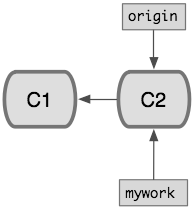
\includegraphics[width=0.20\textwidth]{content/git/rebase0.png}
\end{figure}

Now you do some work, creating two new commits.
\lstset{basicstyle=\scriptsize, numbers=none, captionpos=b, tabsize=4}
\begin{lstlisting}[caption=,language={bash},
breaklines=true,label=lst:]
$ vi file.txt
$ git commit
$ vi otherfile.txt
$ git commit
...
\end{lstlisting}

Meanwhile, someone else does some work creating two new commits on the origin
branch too. This means both 'origin' and 'mywork' has advanced, which means the
work has diverged.

\begin{figure}[h]
\centering
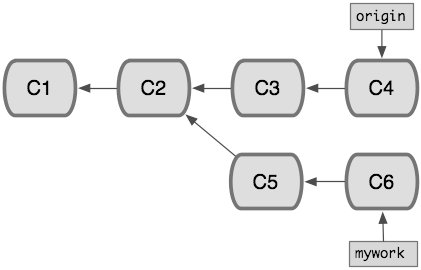
\includegraphics[width=0.43\textwidth]{content/git/rebase1.png}
\end{figure}

At this point, you could use "pull" to merge your changes back in; the result
would create a new merge commit, like this:

\begin{figure}[h]
\centering
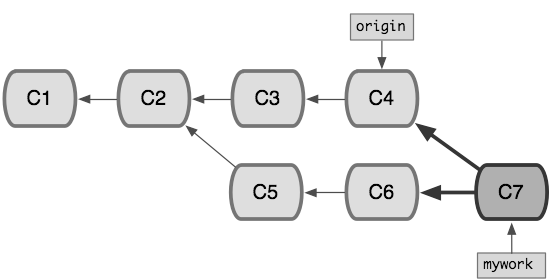
\includegraphics[width=0.43\textwidth]{content/git/rebase2.png}
\end{figure}

However, if you prefer to keep the history in mywork a simple series of commits
without any merges, you may instead choose to use git rebase:

\section{git merge}
\begin{figure}[h]
\centering
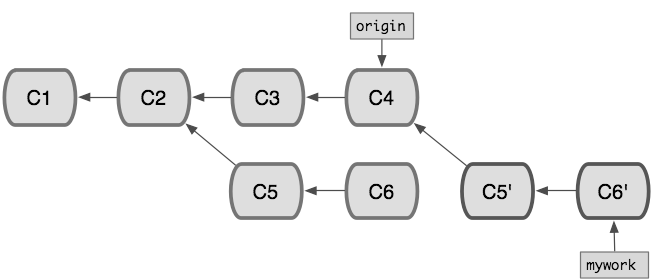
\includegraphics[width=0.43\textwidth]{content/git/rebase3.png}
\end{figure}

\lstset{basicstyle=\scriptsize, numbers=none, captionpos=b, tabsize=4}
\begin{lstlisting}[caption=,language={bash},
breaklines=true,label=lst:]
$ git checkout mywork
$ git rebase origin
\end{lstlisting}

This will remove each of your commits from mywork, temporarily saving them as
patches (in a directory named ".git/rebase"), update mywork to point at the
latest version of origin, then apply each of the saved patches to the new
mywork.

Once the ref ('mywork') is updated to point to the newly created commit
objects, your older commits will be abandoned. They will likely be removed if
you run a pruning garbage collection. (see git gc)
\begin{figure}[h]
\centering
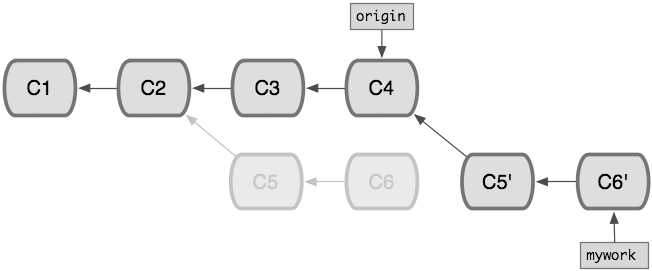
\includegraphics[width=0.43\textwidth]{content/git/rebase4.png}
\end{figure}

So now we can look at the difference in our history between running a merge and
running a rebase:
\begin{figure}[h]
\centering
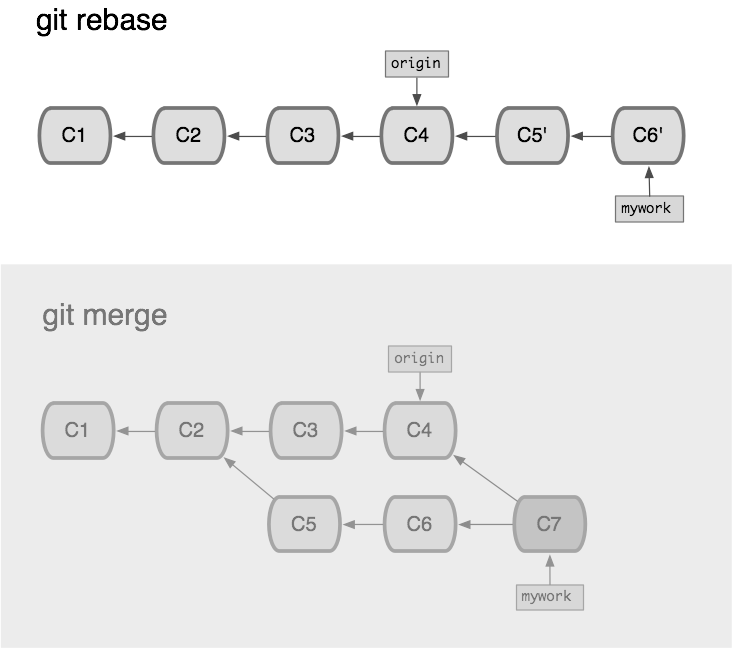
\includegraphics[width=0.43\textwidth]{content/git/rebase5.png}
\end{figure}


In the process of the rebase, it may discover conflicts. In that case it will
stop and allow you to fix the conflicts; after fixing conflicts, use "git-add"
to update the index with those contents, and then, instead of running
git-commit, just run
\lstset{basicstyle=\scriptsize, numbers=none, captionpos=b, tabsize=4}
\begin{lstlisting}[caption=,language={bash},
breaklines=true,label=lst:]
$ git rebase --continue
\end{lstlisting}

and git will continue applying the rest of the patches.

At any point you may use the --abort option to abort this process and return
mywork to the state it had before you started the rebase:

\lstset{basicstyle=\scriptsize, numbers=none, captionpos=b, tabsize=4}
\begin{lstlisting}[caption=,language={bash},
breaklines=true,label=lst:]
$ git rebase --abort
\end{lstlisting}

\subsection{Interactive Rebasing}
You can also rebase interactively. This is often used to re-write your own
commit objects before pusing them somewhere. It is an easy way to split, merge
or re-order commits before sharing them with others. You can also use it to
clean up commits you've pulled from someone when applying them locally.

If you have a number of commits that you would like to somehow modify during
the rebase, you can invoke interactive mode by passing a '-i' or
'--interactive' to the 'git rebase' command.
\lstset{basicstyle=\scriptsize, numbers=none, captionpos=b, tabsize=4}
\begin{lstlisting}[caption=,language={bash},
breaklines=true,label=lst:]
$ git rebase -i origin/master
\end{lstlisting}

This will invoke interactive rebase mode on all the commits you have made since
the last time you have pushed (or merged from the origin repository).

To see what commits those are beforehand, you can run log this way:

\lstset{basicstyle=\scriptsize, numbers=none, captionpos=b, tabsize=4}
\begin{lstlisting}[caption=,language={bash},
breaklines=true,label=lst:]
$ git log github/master..
\end{lstlisting}
Once you run the 'rebase -i' command, you will be thrown into your editor of
choice with something that looks like this:
\lstset{basicstyle=\scriptsize, numbers=none, captionpos=b, tabsize=4}
\begin{lstlisting}[caption=,language={bash},
breaklines=true,label=lst:]
pick fc62e55 added file_size
pick 9824bf4 fixed little thing
pick 21d80a5 added number to log
pick 76b9da6 added the apply command
pick c264051 Revert "added file_size" - not implemented correctly

# Rebase f408319..b04dc3d onto f408319
#
# Commands:
#  p, pick = use commit
#  e, edit = use commit, but stop for amending
#  s, squash = use commit, but meld into previous commit
#
# If you remove a line here THAT COMMIT WILL BE LOST.
# However, if you remove everything, the rebase will be aborted.
#
\end{lstlisting}

This means that there are 5 commits since you last pushed and it gives you one
line per commit with the following format:

(action) (partial-sha) (short commit message)
Now, you can change the action (which is by default 'pick') to either 'edit' or
'squash', or just leave it as 'pick'. You can also reorder the commits just by
moving the lines around however you want. Then, when you exit the editor, git
will try to apply the commits however they are now arranged and do the action
specified.

If 'pick' is specified, it will simply try to apply the patch and save the
commit with the same message as before.

If 'squash' is specified, it will combine that commit with the previous one to
create a new commit. This will drop you into your editor again to merge the
commit messages of the two commits it is now squashing together. So, if you
exit the editor with this:
\lstset{basicstyle=\scriptsize, numbers=none, captionpos=b, tabsize=4}
\begin{lstlisting}[caption=,language={bash},
breaklines=true,label=lst:]
pick   fc62e55 added file_size
squash 9824bf4 fixed little thing
squash 21d80a5 added number to log
squash 76b9da6 added the apply command
squash c264051 Revert "added file_size" - not implemented correctly
\end{lstlisting}

Then you will have to create a single commit message from this:
\lstset{basicstyle=\scriptsize, numbers=none, captionpos=b, tabsize=4}
\begin{lstlisting}[caption=,language={bash},
breaklines=true,label=lst:]
# This is a combination of 5 commits.
# The first commit's message is:
added file_size

# This is the 2nd commit message:

fixed little thing

# This is the 3rd commit message:

added number to log

# This is the 4th commit message:

added the apply command

# This is the 5th commit message:

Revert "added file_size" - not implemented correctly

This reverts commit
fc62e5543b195f18391886b9f663d5a7eca38e84.
\end{lstlisting}

Once you have edited that down into once commit message and exit the editor,
the commit will be saved with your new message.

If 'edit' is specified, it will do the same thing, but then pause before moving
on to the next one and drop you into the command line so you can amend the
commit, or change the commit contents somehow.

If you wanted to split a commit, for instance, you would specify 'edit' for
that commit:
\lstset{basicstyle=\scriptsize, numbers=none, captionpos=b, tabsize=4}
\begin{lstlisting}[caption=,language={bash},
breaklines=true,label=lst:]
pick   fc62e55 added file_size
pick   9824bf4 fixed little thing
edit   21d80a5 added number to log
pick   76b9da6 added the apply command
pick   c264051 Revert "added file_size" - not implemented correctly
\end{lstlisting}

And then when you get to the command line, you revert that commit and create
two (or more) new ones. Lets say 21d80a5 modified two files, file1 and file2,
and you wanted to split them into seperate commits. You could do this after the
rebase dropped you to the command line :
\lstset{basicstyle=\scriptsize, numbers=none, captionpos=b, tabsize=4}
\begin{lstlisting}[caption=,language={bash},
breaklines=true,label=lst:]
$ git reset HEAD^
$ git add file1
$ git commit 'first part of split commit'
$ git add file2
$ git commit 'second part of split commit'
$ git rebase --continue
\end{lstlisting}

And now instead of 5 commits, you would have 6.

The last useful thing that interactive rebase can do is drop commits for you.
If instead of choosing 'pick', 'squash' or 'edit' for the commit line, you
simply remove the line, it will remove the commit from the history.

\section{Interactive Adding}
Interactive Adding is a really nice way of working with and visualizing the Git
index. To start it up, simply type 'git add -i'. Git will show you all the
modified files you have and their status.
\lstset{basicstyle=\scriptsize, numbers=none, captionpos=b, tabsize=4}
\begin{lstlisting}[caption=,language={bash},
breaklines=true,label=lst:]
$>git add -i
           staged     unstaged path
  1:    unchanged        +4/-0 assets/stylesheets/style.css
  2:    unchanged      +23/-11 layout/book_index_template.html
  3:    unchanged        +7/-7 layout/chapter_template.html
  4:    unchanged        +3/-3 script/pdf.rb
  5:    unchanged      +121/-0 text/14_Interactive_Rebasing/0_ Interactive_Rebasing.markdown

*** Commands ***
  1: status   2: update   3: revert   4: add untracked
  5: patch    6: diff     7: quit     8: help
What now> 
\end{lstlisting}

In this case, we can see that there are 5 modified files that have not been
added to our index yet (unstaged), and even how many lines have been added to
or removed from each. It then shows us an interactive menu of what we can do in
this mode.

If we want to stage the files, we can type '2' or 'u' for the update mode. Then
I can specify which files I want to stage (add to the index) by typing in the
numbers of the files (in this case, 1-4)
\lstset{basicstyle=\scriptsize, numbers=none, captionpos=b, tabsize=4}
\begin{lstlisting}[caption=,language={bash},
breaklines=true,label=lst:]
What now> 2
           staged     unstaged path
  1:    unchanged        +4/-0 assets/stylesheets/style.css
  2:    unchanged      +23/-11 layout/book_index_template.html
  3:    unchanged        +7/-7 layout/chapter_template.html
  4:    unchanged        +3/-3 script/pdf.rb
  5:    unchanged      +121/-0 text/14_Interactive_Rebasing/0_ Interactive_Rebasing.markdown
Update>> 1-4
           staged     unstaged path
* 1:    unchanged        +4/-0 assets/stylesheets/style.css
* 2:    unchanged      +23/-11 layout/book_index_template.html
* 3:    unchanged        +7/-7 layout/chapter_template.html
* 4:    unchanged        +3/-3 script/pdf.rb
  5:    unchanged      +121/-0 text/14_Interactive_Rebasing/0_ Interactive_Rebasing.markdown
Update>> 
\end{lstlisting}

If I hit enter, I will be taken back to the main menu where I can see that the file status has changed:
\lstset{basicstyle=\scriptsize, numbers=none, captionpos=b, tabsize=4}
\begin{lstlisting}[caption=,language={bash},
breaklines=true,label=lst:]
What now> status
           staged     unstaged path
  1:        +4/-0      nothing assets/stylesheets/style.css
  2:      +23/-11      nothing layout/book_index_template.html
  3:        +7/-7      nothing layout/chapter_template.html
  4:        +3/-3      nothing script/pdf.rb
  5:    unchanged      +121/-0 text/14_Interactive_Rebasing/0_ Interactive_Rebasing.markdown
\end{lstlisting}

Now we can see the first four files are staged and the last one is still not.
This is basically a compressed way to see the same information we see when we
run 'git status' from the command line:
\lstset{basicstyle=\scriptsize, numbers=none, captionpos=b, tabsize=4}
\begin{lstlisting}[caption=,language={bash},
breaklines=true,label=lst:]
$ git status
# On branch master
# Changes to be committed:
#   (use "git reset HEAD <file>..." to unstage)
#
#   modified:   assets/stylesheets/style.css
#   modified:   layout/book_index_template.html
#   modified:   layout/chapter_template.html
#   modified:   script/pdf.rb
#
# Changed but not updated:
#   (use "git add <file>..." to update what will be committed)
#
#   modified:   text/14_Interactive_Rebasing/0_ Interactive_Rebasing.markdown
#
\end{lstlisting}

There are a number of useful things we can do, including unstaging files (3:
revert), adding untracked files (4: add untracked), and viewing diffs (6:
diff). Those are all pretty straightforward. However, there is one command that
is pretty cool here, which is staging patches (5: patch).

If you type '5' or 'p' in the menu, git will show you your diff patch by patch
(or hunk by hunk) and ask if you want to stage each one. That way you can
actually stage for a commit a part of a file edit. If you've edited a file and
want to only commit part of it and not an unfinished part, or commit
documentation or whitespace changes seperate from substantive changes, you can
use 'git add -i' to do so relatively easily.

Here I've staged some changes to the book\_index\_template.html file, but not all
of them:
\lstset{basicstyle=\scriptsize, numbers=none, captionpos=b, tabsize=4}
\begin{lstlisting}[caption=,language={bash},
breaklines=true,label=lst:]
         staged     unstaged path
1:        +4/-0      nothing assets/stylesheets/style.css
2:       +20/-7        +3/-4 layout/book_index_template.html
3:        +7/-7      nothing layout/chapter_template.html
4:        +3/-3      nothing script/pdf.rb
5:    unchanged      +121/-0 text/14_Interactive_Rebasing/0_ Interactive_Rebasing.markdown
6:    unchanged       +85/-0 text/15_Interactive_Adding/0_ Interactive_Adding.markdown
\end{lstlisting}

When you are done making changes to your index through 'git add -i', you simply
quit (7: quit) and then run 'git commit' to commit the staged changes. Remember
not to run 'git commit -a', which will blow away all the careful changes you've
just made and simply commit everything.

\subsection{Stashing}
While you are in the middle of working on something complicated, you find an
unrelated but obvious and trivial bug. You would like to fix it before
continuing. You can use git stash to save the current state of your work, and
after fixing the bug (or, optionally after doing so on a different branch and
then coming back), unstash the work-in-progress changes.
\lstset{basicstyle=\scriptsize, numbers=none, captionpos=b, tabsize=4}
\begin{lstlisting}[caption=,language={bash},
breaklines=true,label=lst:]
$ git stash "work in progress for foo feature"
\end{lstlisting}

This command will save your changes away to the stash, and reset your working
tree and the index to match the tip of your current branch. Then you can make
your fix as usual.
\lstset{basicstyle=\scriptsize, numbers=none, captionpos=b, tabsize=4}
\begin{lstlisting}[caption=,language={bash},
breaklines=true,label=lst:]
... edit and test ...
$ git commit -a -m "blorpl: typofix"
\end{lstlisting}

After that, you can go back to what you were working on with git stash apply:
\lstset{basicstyle=\scriptsize, numbers=none, captionpos=b, tabsize=4}
\begin{lstlisting}[caption=,language={bash},
breaklines=true,label=lst:]
$ git stash apply
\end{lstlisting}

\subsubsection{Stash Queue}
You can also use stashing to queue up stashed changes.  If you run 'git stash
list' you can see which stashes you have saved:
\lstset{basicstyle=\scriptsize, numbers=none, captionpos=b, tabsize=4}
\begin{lstlisting}[caption=,language={bash},
breaklines=true,label=lst:]
$>git stash list
stash@{0}: WIP on book: 51bea1d... fixed images
stash@{1}: WIP on master: 9705ae6... changed the browse code to the official repo
\end{lstlisting}

Then you can apply them individually with 'git stash apply stash@{1}'. You can
clear out the list with 'git stash clear'.

\subsection{Git Treeishes}
There are a number of ways to refer to a particular commit or tree other than
spelling out the entire 40-character sha. In Git, these are referred to as a
'treeish'.

\subsubsection{Partial Sha}
If your commit sha is '980e3ccdaac54a0d4de358f3fe5d718027d96aae', git will
recognize any of the following identically:
\lstset{basicstyle=\scriptsize, numbers=none, captionpos=b, tabsize=4}
\begin{lstlisting}[caption=,language={bash},
breaklines=true,label=lst:]
980e3ccdaac54a0d4de358f3fe5d718027d96aae
980e3ccdaac54a0d4
980e3cc
\end{lstlisting}

As long as the partial sha is unique - it can't be confused with another (which
is incredibly unlikely if you use at least 5 characters), git will expand a
partial sha for you.

\subsubsection{Branch, Remote or Tag Name}
You can always use a branch, remote or tag name instead of a sha, since they
are simply pointers anyhow. If your master branch is on the 980e3 commit and
you've pushed it to origin and have tagged it 'v1.0', then all of the following
are equivalent:
\lstset{basicstyle=\scriptsize, numbers=none, captionpos=b, tabsize=4}
\begin{lstlisting}[caption=,language={bash},
breaklines=true,label=lst:]

980e3ccdaac54a0d4de358f3fe5d718027d96aae
origin/master
refs/remotes/origin/master
master
refs/heads/master
v1.0
refs/tags/v1.0
\end{lstlisting}

Which means the following will give you identical output:
\lstset{basicstyle=\scriptsize, numbers=none, captionpos=b, tabsize=4}
\begin{lstlisting}[caption=,language={bash},
breaklines=true,label=lst:]
$ git log master

$ git log refs/tags/v1.0
\end{lstlisting}

\subsubsection{Date Spec}
The Ref Log that git keeps will allow you to do some relative stuff locally,
such as:
\lstset{basicstyle=\scriptsize, numbers=none, captionpos=b, tabsize=4}
\begin{lstlisting}[caption=,language={bash},
breaklines=true,label=lst:]
master@{yesterday}

master@{1 month ago}
\end{lstlisting}

Which is shorthand for 'where the master branch head was yesterday', etc. Note
that this format can result in different shas on different computers, even if
the master branch is currently pointing to the same place.

\subsubsection{Ordinal Spec}
This format will give you the Nth previous value of a particular reference. For
example:
\lstset{basicstyle=\scriptsize, numbers=none, captionpos=b, tabsize=4}
\begin{lstlisting}[caption=,language={bash},
breaklines=true,label=lst:]
master@{5}
\end{lstlisting}

will give you the 5th prior value of the master head ref.

\subsubsection{Carrot Parent}
This will give you the Nth parent of a particular commit. This format is only
useful on merge commits - commit objects that have more than one direct parent.
\lstset{basicstyle=\scriptsize, numbers=none, captionpos=b, tabsize=4}
\begin{lstlisting}[caption=,language={bash},
breaklines=true,label=lst:]
master^2
\end{lstlisting}

\subsubsection{Tilde Spec}
The tilde spec will give you the Nth grandparent of a commit object. For
example,
\lstset{basicstyle=\scriptsize, numbers=none, captionpos=b, tabsize=4}
\begin{lstlisting}[caption=,language={bash},
breaklines=true,label=lst:]
master~2
\end{lstlisting}

will give us the first parent of the first parent of the commit that master
points to. It is equivalent to:
\lstset{basicstyle=\scriptsize, numbers=none, captionpos=b, tabsize=4}
\begin{lstlisting}[caption=,language={bash},
breaklines=true,label=lst:]
master^^
\end{lstlisting}

You can keep doing this, too. The following specs will point to the same
commit:
\lstset{basicstyle=\scriptsize, numbers=none, captionpos=b, tabsize=4}
\begin{lstlisting}[caption=,language={bash},
breaklines=true,label=lst:]
master^^^^^^
master~3^~2
master~6
\end{lstlisting}

\subsubsection{Tree Pointer}
This disambiguates a commit from the tree that it points to. If you want the
sha that a commit points to, you can add the '\^{tree}' spec to the end of it.
\lstset{basicstyle=\scriptsize, numbers=none, captionpos=b, tabsize=4}
\begin{lstlisting}[caption=,language={bash},
breaklines=true,label=lst:]
master^{tree}
\end{lstlisting}

\subsubsection{Blob Spec}
If you want the sha of a particular blob, you can add the blob path at the end
of the treeish, like so:
\lstset{basicstyle=\scriptsize, numbers=none, captionpos=b, tabsize=4}
\begin{lstlisting}[caption=,language={bash},
breaklines=true,label=lst:]
master:/path/to/file
\end{lstlisting}

\subsubsection{Range}
Finally, you can specify a range of commits with the range spec. This will give
you all the commits between 7b593b5 and 51bea1 (where 51bea1 is most recent),
excluding 7b593b5 but including 51bea1:
\lstset{basicstyle=\scriptsize, numbers=none, captionpos=b, tabsize=4}
\begin{lstlisting}[caption=,language={bash},
breaklines=true,label=lst:]
7b593b5..51bea1
\end{lstlisting}

This will include every commit since 7b593b:
\lstset{basicstyle=\scriptsize, numbers=none, captionpos=b, tabsize=4}
\begin{lstlisting}[caption=,language={bash},
breaklines=true,label=lst:]
7b593b.. 
\end{lstlisting}

\section{Tracking Branches}
A 'tracking branch' in Git is a local branch that is connected to a remote
branch. When you push and pull on that branch, it automatically pushes and
pulls to the remote branch that it is connected with.

Use this if you always pull from the same upstream branch into the new branch,
and if you don't want to use "git pull " explicitly.

The 'git clone' command automatically sets up a 'master' branch that is a
tracking branch for 'origin/master' - the master branch on the cloned
repository.

You can create a tracking branch manually by adding the '--track' option to the
'branch' command in Git.
\lstset{basicstyle=\scriptsize, numbers=none, captionpos=b, tabsize=4}
\begin{lstlisting}[caption=,language={bash},
breaklines=true,label=lst:]
git branch --track experimental origin/experimental
\end{lstlisting}

Then when you run:
\lstset{basicstyle=\scriptsize, numbers=none, captionpos=b, tabsize=4}
\begin{lstlisting}[caption=,language={bash},
breaklines=true,label=lst:]
$ git pull experimental
\end{lstlisting}

It will automatically fetch from 'origin' and merge 'origin/experimental' into
your local 'experimental' branch.

Likewise, when you push to origin, it will push what your 'experimental' points
to to origins 'experimental', without having to specify it.

\subsection{Finding with Git Grep}
Finding files with words or phrases in Git is really easy with the git grep
command. It is possible to do this with the normal unix 'grep' command, but
with 'git grep' you can also search through previous versions of the project
without having to check them out.

For example, if I wanted to see every place that used the 'xmmap' call in my
git.git repository, I could run this:
\lstset{basicstyle=\scriptsize, numbers=none, captionpos=b, tabsize=4}
\begin{lstlisting}[caption=,language={bash},
breaklines=true,label=lst:]
$ git grep xmmap
config.c:               contents = xmmap(NULL, contents_sz, PROT_READ,
diff.c:         s->data = xmmap(NULL, s->size, PROT_READ, MAP_PRIVATE, fd, 0);
git-compat-util.h:extern void *xmmap(void *start, size_t length, int prot, int fla
read-cache.c:   mmap = xmmap(NULL, mmap_size, PROT_READ | PROT_WRITE, MAP_PRIVATE,
refs.c: log_mapped = xmmap(NULL, mapsz, PROT_READ, MAP_PRIVATE, logfd, 0);
sha1_file.c:    map = xmmap(NULL, mapsz, PROT_READ, MAP_PRIVATE, fd, 0);
sha1_file.c:    idx_map = xmmap(NULL, idx_size, PROT_READ, MAP_PRIVATE, fd, 0);
sha1_file.c:                    win->base = xmmap(NULL, win->len,
sha1_file.c:                    map = xmmap(NULL, *size, PROT_READ, MAP_PRIVATE, f
sha1_file.c:            buf = xmmap(NULL, size, PROT_READ, MAP_PRIVATE, fd, 0);
wrapper.c:void *xmmap(void *start, size_t length,
\end{lstlisting}

If I wanted to see the line number of each match as well, I can add the '-n'
option:
\lstset{basicstyle=\scriptsize, numbers=none, captionpos=b, tabsize=4}
\begin{lstlisting}[caption=,language={bash},
breaklines=true,label=lst:]
$>git grep -n xmmap
config.c:1016:          contents = xmmap(NULL, contents_sz, PROT_READ,
diff.c:1833:            s->data = xmmap(NULL, s->size, PROT_READ, MAP_PRIVATE, fd,
git-compat-util.h:291:extern void *xmmap(void *start, size_t length, int prot, int
read-cache.c:1178:      mmap = xmmap(NULL, mmap_size, PROT_READ | PROT_WRITE, MAP_
refs.c:1345:    log_mapped = xmmap(NULL, mapsz, PROT_READ, MAP_PRIVATE, logfd, 0);
sha1_file.c:377:        map = xmmap(NULL, mapsz, PROT_READ, MAP_PRIVATE, fd, 0);
sha1_file.c:479:        idx_map = xmmap(NULL, idx_size, PROT_READ, MAP_PRIVATE, fd
sha1_file.c:780:                        win->base = xmmap(NULL, win->len,
sha1_file.c:1076:                       map = xmmap(NULL, *size, PROT_READ, MAP_PR
sha1_file.c:2393:               buf = xmmap(NULL, size, PROT_READ, MAP_PRIVATE, fd
wrapper.c:89:void *xmmap(void *start, size_t length,
\end{lstlisting}

If we're only interested in the filename, we can pass the '--name-only' option:
\lstset{basicstyle=\scriptsize, numbers=none, captionpos=b, tabsize=4}
\begin{lstlisting}[caption=,language={bash},
breaklines=true,label=lst:]
$>git grep --name-only xmmap
config.c
diff.c
git-compat-util.h
read-cache.c
refs.c
sha1_file.c
wrapper.c
\end{lstlisting}

We could also see how many line matches we have in each file with the '-c'
option:
\lstset{basicstyle=\scriptsize, numbers=none, captionpos=b, tabsize=4}
\begin{lstlisting}[caption=,language={bash},
breaklines=true,label=lst:]
$>git grep -c xmmap
config.c:1
diff.c:1
git-compat-util.h:1
read-cache.c:1
refs.c:1
sha1_file.c:5
wrapper.c:1
\end{lstlisting}

Now, if I wanted to see where that was used in a specific version of git, I
could add the tag reference to the end, like this:
\lstset{basicstyle=\scriptsize, numbers=none, captionpos=b, tabsize=4}
\begin{lstlisting}[caption=,language={bash},
breaklines=true,label=lst:]
$ git grep xmmap v1.5.0
v1.5.0:config.c:                contents = xmmap(NULL, st.st_size, PROT_READ,
v1.5.0:diff.c:          s->data = xmmap(NULL, s->size, PROT_READ, MAP_PRIVATE, fd,
v1.5.0:git-compat-util.h:static inline void *xmmap(void *start, size_t length,
v1.5.0:read-cache.c:                    cache_mmap = xmmap(NULL, cache_mmap_size, 
v1.5.0:refs.c:  log_mapped = xmmap(NULL, st.st_size, PROT_READ, MAP_PRIVATE, logfd
v1.5.0:sha1_file.c:     map = xmmap(NULL, st.st_size, PROT_READ, MAP_PRIVATE, fd, 
v1.5.0:sha1_file.c:     idx_map = xmmap(NULL, idx_size, PROT_READ, MAP_PRIVATE, fd
v1.5.0:sha1_file.c:                     win->base = xmmap(NULL, win->len,
v1.5.0:sha1_file.c:     map = xmmap(NULL, st.st_size, PROT_READ, MAP_PRIVATE, fd, 
v1.5.0:sha1_file.c:             buf = xmmap(NULL, size, PROT_READ, MAP_PRIVATE, fd
\end{lstlisting}

We can see that there are some differences between the current lines and these
lines in version 1.5.0, one of which is that xmmap is now used in wrapper.c
where it was not back in v1.5.0.

We can also combine search terms in grep. Say we wanted to search for where
SORT\_DIRENT is defined in our repository:
\lstset{basicstyle=\scriptsize, numbers=none, captionpos=b, tabsize=4}
\begin{lstlisting}[caption=,language={bash},
breaklines=true,label=lst:]
$ git grep -e '#define' --and -e SORT_DIRENT
builtin-fsck.c:#define SORT_DIRENT 0
builtin-fsck.c:#define SORT_DIRENT 1
\end{lstlisting}

We can also search for every file that has both search terms, but display each
line that has either of the terms in those files:
\lstset{basicstyle=\scriptsize, numbers=none, captionpos=b, tabsize=4}
\begin{lstlisting}[caption=,language={bash},
breaklines=true,label=lst:]
$ git grep --all-match -e '#define' -e SORT_DIRENT
builtin-fsck.c:#define REACHABLE 0x0001
builtin-fsck.c:#define SEEN      0x0002
builtin-fsck.c:#define ERROR_OBJECT 01
builtin-fsck.c:#define ERROR_REACHABLE 02
builtin-fsck.c:#define SORT_DIRENT 0
builtin-fsck.c:#define DIRENT_SORT_HINT(de) 0
builtin-fsck.c:#define SORT_DIRENT 1
builtin-fsck.c:#define DIRENT_SORT_HINT(de) ((de)->d_ino)
builtin-fsck.c:#define MAX_SHA1_ENTRIES (1024)
builtin-fsck.c: if (SORT_DIRENT)
\end{lstlisting}

We can also search for lines that have one term and either of two other terms,
for example, if we wanted to see where we defined constants that had either
PATH or MAX in the name:
\lstset{basicstyle=\scriptsize, numbers=none, captionpos=b, tabsize=4}
\begin{lstlisting}[caption=,language={bash},
breaklines=true,label=lst:]
$ git grep -e '#define' --and \( -e PATH -e MAX \) 
abspath.c:#define MAXDEPTH 5
builtin-blame.c:#define MORE_THAN_ONE_PATH      (1u<<13)
builtin-blame.c:#define MAXSG 16
builtin-describe.c:#define MAX_TAGS     (FLAG_BITS - 1)
builtin-fetch-pack.c:#define MAX_IN_VAIN 256
builtin-fsck.c:#define MAX_SHA1_ENTRIES (1024)
...
\end{lstlisting}

\section{Undoing in Git - Reset, Checkout and Revert}
Git provides multiple methods for fixing up mistakes as you are developing.
Selecting an appropriate method depends on whether or not you have committed
the mistake, and if you have committed the mistake, whether you have shared the
erroneous commit with anyone else.

\subsection{Fixing un-committed mistakes}
If you've messed up the working tree, but haven't yet committed your mistake,
you can return the entire working tree to the last committed state with
\lstset{basicstyle=\scriptsize, numbers=none, captionpos=b, tabsize=4}
\begin{lstlisting}[caption=,language={bash},
breaklines=true,label=lst:]
$ git reset --hard HEAD
\end{lstlisting}

This will throw away any changes you may have added to the git index and as
well as any outstanding changes you have in your working tree. In other words,
it causes the results of "git diff" and "git diff --cached" to both be empty.

If you just want to restore just one file, say your hello.rb, use git checkout
instead
\lstset{basicstyle=\scriptsize, numbers=none, captionpos=b, tabsize=4}
\begin{lstlisting}[caption=,language={bash},
breaklines=true,label=lst:]
$ git checkout -- hello.rb
$ git checkout HEAD hello.rb
\end{lstlisting}

The first command restores hello.rb to the version in the index, so that "git
diff hello.rb" returns no differences. The second command will restore hello.rb
to the version in the HEAD revision, so that both "git diff hello.rb" and "git
diff --cached hello.rb" return no differences.

\subsection{Fixing committed mistakes}
If you make a commit that you later wish you hadn't, there are two
fundamentally different ways to fix the problem:
\begin{enumerate}
\item You can create a new commit that undoes whatever was done by the old commit.
This is the correct thing if your mistake has already been made public.

\item You can go back and modify the old commit. You should never do this if you have
already made the history public; git does not normally expect the "history" of
a project to change, and cannot correctly perform repeated merges from a branch
that has had its history changed.
\end{enumerate}

\subsection{Fixing a mistake with a new commit}
Creating a new commit that reverts an earlier change is very easy; just pass
the git revert command a reference to the bad commit; for example, to revert
the most recent commit:
\lstset{basicstyle=\scriptsize, numbers=none, captionpos=b, tabsize=4}
\begin{lstlisting}[caption=,language={bash},
breaklines=true,label=lst:]
$ git revert HEAD
\end{lstlisting}

This will create a new commit which undoes the change in HEAD. You will be
given a chance to edit the commit message for the new commit.

You can also revert an earlier change, for example, the next-to-last:
\lstset{basicstyle=\scriptsize, numbers=none, captionpos=b, tabsize=4}
\begin{lstlisting}[caption=,language={bash},
breaklines=true,label=lst:]
$ git revert HEAD^
\end{lstlisting}

In this case git will attempt to undo the old change while leaving intact any
changes made since then. If more recent changes overlap with the changes to be
reverted, then you will be asked to fix conflicts manually, just as in the case
of resolving a merge.

\subsection{Fixing a mistake by modifying a commit}
If you have just committed something but realize you need to fix up that
commit, recent versions of git commit support an --amend flag which instructs
git to replace the HEAD commit with a new one, based on the current contents of
the index. This gives you an opportunity to add files that you forgot to add or
correct typos in a commit message, prior to pushing the change out for the
world to see.

If you find a mistake in an older commit, but still one that you have not yet
published to the world, you use git rebase in interactive mode, with "git
rebase -i" marking the change that requires correction with edit. This will
allow you to amend the commit during the rebasing process.

\subsection{Maintaining Git}
Ensuring good performance

On large repositories, git depends on compression to keep the history
information from taking up too much space on disk or in memory.

This compression is not performed automatically. Therefore you should
occasionally run git gc:
\lstset{basicstyle=\scriptsize, numbers=none, captionpos=b, tabsize=4}
\begin{lstlisting}[caption=,language={bash},
breaklines=true,label=lst:]
$ git gc
\end{lstlisting}

to recompress the archive. This can be very time-consuming, so you may prefer
to run git-gc when you are not doing other work.

\subsubsection{Ensuring reliability}
The git fsck command runs a number of self-consistency checks on the
repository, and reports on any problems. This may take some time. The most
common warning by far is about "dangling" objects:
\lstset{basicstyle=\scriptsize, numbers=none, captionpos=b, tabsize=4}
\begin{lstlisting}[caption=,language={bash},
breaklines=true,label=lst:]
$ git fsck
dangling commit 7281251ddd2a61e38657c...
dangling commit 2706a059f258c6b245f29...
dangling commit 13472b7c4b80851a1bc55...
dangling blob 218761f9d90712d37a9c5e3...
dangling commit bf093535a34a4d35731aa...
dangling commit 8e4bec7f2ddaa268bef99...
dangling tree d50bb86186bf27b681d25af...
dangling tree b24c2473f1fd3d91352a624...
...
\end{lstlisting}

Dangling objects are not a problem. At worst they may take up a little extra
disk space. They can sometimes provide a last-resort method for recovering lost
work.

\subsection{Setting Up A Public Repository}
Assume your personal repository is in the directory ~/proj. We first create a
new clone of the repository and tell git-daemon that it is meant to be public:
\lstset{basicstyle=\scriptsize, numbers=none, captionpos=b, tabsize=4}
\begin{lstlisting}[caption=,language={bash},
breaklines=true,label=lst:]
$ git clone --bare ~/proj proj.git
$ touch proj.git/git-daemon-export-ok
\end{lstlisting}

The resulting directory proj.git contains a "bare" git repository--it is just
the contents of the ".git" directory, without any files checked out around it.

Next, copy proj.git to the server where you plan to host the public repository.
You can use scp, rsync, or whatever is most convenient.

\subsubsection{Exporting a git repository via the git protocol}
This is the preferred method.

If someone else administers the server, they should tell you what directory to
put the repository in, and what git:// URL it will appear at.

Otherwise, all you need to do is start git daemon; it will listen on port 9418.
By default, it will allow access to any directory that looks like a git
directory and contains the magic file git-daemon-export-ok. Passing some
directory paths as git-daemon arguments will further restrict the exports to
those paths.

You can also run git-daemon as an inetd service; see the git daemon man page
for details. (See especially the examples section.)

\subsubsection{Exporting a git repository via http}
The git protocol gives better performance and reliability, but on a host with a
web server set up, http exports may be simpler to set up.

All you need to do is place the newly created bare git repository in a
directory that is exported by the web server, and make some adjustments to give
web clients some extra information they need:
\lstset{basicstyle=\scriptsize, numbers=none, captionpos=b, tabsize=4}
\begin{lstlisting}[caption=,language={bash},
breaklines=true,label=lst:]
$ mv proj.git /home/you/public_html/proj.git
$ cd proj.git
$ git --bare update-server-info
$ chmod a+x hooks/post-update
\end{lstlisting}

(For an explanation of the last two lines, see git update-server-info and
githooks.)

Advertise the URL of proj.git. Anybody else should then be able to clone or
pull from that URL, for example with a command line like:
\lstset{basicstyle=\scriptsize, numbers=none, captionpos=b, tabsize=4}
\begin{lstlisting}[caption=,language={bash},
breaklines=true,label=lst:]
$ git clone http://yourserver.com/~you/proj.git
\end{lstlisting}

\subsection{Setting Up a Private Repository}
If you need to setup a private repository and want to do so locally, rather
than using a hosted solution, you have a number of options.

\subsubsection{Repo Access over SSH}
Generally, the easiest solution is to simply use Git over SSH. If users already
have ssh accounts on a machine, you can put the git repository anywhere on the
box that they have access to and let them access it over normal ssh logins. For
example, say you have a repository you want to host. You can export it as a
bare repo and then scp it onto your server like so:
\lstset{basicstyle=\scriptsize, numbers=none, captionpos=b, tabsize=4}
\begin{lstlisting}[caption=,language={bash},
breaklines=true,label=lst:]
$ git clone --bare /home/user/myrepo/.git /tmp/myrepo.git
$ scp -r /tmp/myrepo.git myserver.com:/opt/git/myrepo.git
\end{lstlisting}

Then someone else with an ssh account on myserver.com can clone via:
\lstset{basicstyle=\scriptsize, numbers=none, captionpos=b, tabsize=4}
\begin{lstlisting}[caption=,language={bash},
breaklines=true,label=lst:]
$ git clone myserver.com:/opt/git/myrepo.git
\end{lstlisting}

Which will simply prompt them for thier ssh password or use thier public key,
however they have ssh authentication setup.

\section{Advanced Git}
\section{Advanced Branching And Merging}
\subsection{Getting conflict-resolution help during a merge}

All of the changes that git was able to merge automatically are already added
to the index file, so git diff shows only the conflicts. It uses an unusual
syntax:
\lstset{basicstyle=\scriptsize, numbers=none, captionpos=b, tabsize=4}
\begin{lstlisting}[caption=,language={bash},
breaklines=true,label=lst:]
$ git diff
diff --cc file.txt
index 802992c,2b60207..0000000
--- a/file.txt
+++ b/file.txt
@@@ -1,1 -1,1 +1,5 @@@
++<<<<<<< HEAD:file.txt
 +Hello world
++=======
+ Goodbye
++>>>>>>> 77976da35a11db4580b80ae27e8d65caf5208086:file.txt
\end{lstlisting}

Recall that the commit which will be committed after we resolve this conflict
will have two parents instead of the usual one: one parent will be HEAD, the
tip of the current branch; the other will be the tip of the other branch, which
is stored temporarily in MERGE\_HEAD.

During the merge, the index holds three versions of each file. Each of these
three "file stages" represents a different version of the file:
\lstset{basicstyle=\scriptsize, numbers=none, captionpos=b, tabsize=4}
\begin{lstlisting}[caption=,language={bash},
breaklines=true,label=lst:]
$ git show :1:file.txt  # the file in a common ancestor of both branches
$ git show :2:file.txt  # the version from HEAD.
$ git show :3:file.txt  # the version from MERGE_HEAD.
\end{lstlisting}

When you ask git diff to show the conflicts, it runs a three-way diff between
the conflicted merge results in the work tree with stages 2 and 3 to show only
hunks whose contents come from both sides, mixed (in other words, when a hunk's
merge results come only from stage 2, that part is not conflicting and is not
shown. Same for stage 3).

The diff above shows the differences between the working-tree version of
file.txt and the stage 2 and stage 3 versions. So instead of preceding each
line by a single "+" or "-", it now uses two columns: the first column is used
for differences between the first parent and the working directory copy, and
the second for differences between the second parent and the working directory
copy. (See the "COMBINED DIFF FORMAT" section of git diff-files for a details
of the format.)

After resolving the conflict in the obvious way (but before updating the
index), the diff will look like:
\lstset{basicstyle=\scriptsize, numbers=none, captionpos=b, tabsize=4}
\begin{lstlisting}[caption=,language={bash},
breaklines=true,label=lst:]
$ git diff
diff --cc file.txt
index 802992c,2b60207..0000000
--- a/file.txt
+++ b/file.txt
@@@ -1,1 -1,1 +1,1 @@@
- Hello world
-Goodbye
++Goodbye world
\end{lstlisting}

This shows that our resolved version deleted "Hello world" from the first
parent, deleted "Goodbye" from the second parent, and added "Goodbye world",
which was previously absent from both.

Some special diff options allow diffing the working directory against any of
these stages:
\lstset{basicstyle=\scriptsize, numbers=none, captionpos=b, tabsize=4}
\begin{lstlisting}[caption=,language={bash},
breaklines=true,label=lst:]
$ git diff -1 file.txt      # diff against stage 1
$ git diff --base file.txt  # same as the above
$ git diff -2 file.txt      # diff against stage 2
$ git diff --ours file.txt  # same as the above
$ git diff -3 file.txt      # diff against stage 3
$ git diff --theirs file.txt    # same as the above.
\end{lstlisting}

The git log and gitk commands also provide special help for merges:
\lstset{basicstyle=\scriptsize, numbers=none, captionpos=b, tabsize=4}
\begin{lstlisting}[caption=,language={bash},
breaklines=true,label=lst:]
$ git log --merge
$ gitk --merge
\end{lstlisting}

These will display all commits which exist only on HEAD or on MERGE\_HEAD, and
which touch an unmerged file.

You may also use git mergetool, which lets you merge the unmerged files using
external tools such as emacs or kdiff3.

Each time you resolve the conflicts in a file and update the index:
\lstset{basicstyle=\scriptsize, numbers=none, captionpos=b, tabsize=4}
\begin{lstlisting}[caption=,language={bash},
breaklines=true,label=lst:]
$ git add file.txt
\end{lstlisting}

the different stages of that file will be "collapsed", after which git-diff
will (by default) no longer show diffs for that file.

\subsection{Multiway Merge}
You can merge several heads at one time by simply listing them on the same git
merge command. For instance,
\lstset{basicstyle=\scriptsize, numbers=none, captionpos=b, tabsize=4}
\begin{lstlisting}[caption=,language={bash},
breaklines=true,label=lst:]
$ git merge scott/master rick/master tom/master
\end{lstlisting}

is the equivalent of:
\lstset{basicstyle=\scriptsize, numbers=none, captionpos=b, tabsize=4}
\begin{lstlisting}[caption=,language={bash},
breaklines=true,label=lst:]
$ git merge scott/master
$ git merge rick/master
$ git merge tom/master
\end{lstlisting}

\subsection{Subtree}
There are situations where you want to include contents in your project from an
independently developed project. You can just pull from the other project as
long as there are no conflicting paths.

The problematic case is when there are conflicting files. Potential candidates
are Makefiles and other standard filenames. You could merge these files but
probably you do not want to. A better solution for this problem can be to merge
the project as its own subdirectory. This is not supported by the recursive
merge strategy, so just pulling won't work.

What you want is the subtree merge strategy, which helps you in such a
situation.

In this example, let's say you have the repository at /path/to/B (but it can be
an URL as well, if you want). You want to merge the master branch of that
repository to the dir-B subdirectory in your current branch.

Here is the command sequence you need:
\lstset{basicstyle=\scriptsize, numbers=none, captionpos=b, tabsize=4}
\begin{lstlisting}[caption=,language={bash},
breaklines=true,label=lst:]
$ git remote add -f Bproject /path/to/B (1)
$ git merge -s ours --no-commit Bproject/master (2)
$ git read-tree --prefix=dir-B/ -u Bproject/master (3)
$ git commit -m "Merge B project as our subdirectory" (4)
$ git pull -s subtree Bproject master (5)
\end{lstlisting}

The benefit of using subtree merge is that it requires less administrative
burden from the users of your repository. It works with older (before Git
v1.5.2) clients and you have the code right after clone.

However if you use submodules then you can choose not to transfer the submodule
objects. This may be a problem with the subtree merge.

Also, in case you make changes to the other project, it is easier to submit
changes if you just use submodules.

\section{Finding Issues - Git Bisect}
Suppose version 2.6.18 of your project worked, but the version at "master"
crashes. Sometimes the best way to find the cause of such a regression is to
perform a brute-force search through the project's history to find the
particular commit that caused the problem. The git bisect command can help you
do this:
\lstset{basicstyle=\scriptsize, numbers=none, captionpos=b, tabsize=4}
\begin{lstlisting}[caption=,language={bash},
breaklines=true,label=lst:]
$ git bisect start
$ git bisect good v2.6.18
$ git bisect bad master
Bisecting: 3537 revisions left to test after this
[65934a9a028b88e83e2b0f8b36618fe503349f8e] BLOCK: Make USB storage depend on SCSI rather than selecting it [try #6]
\end{lstlisting}

If you run "git branch" at this point, you'll see that git has temporarily
moved you to a new branch named "bisect". This branch points to a commit (with
commit id 65934...) that is reachable from "master" but not from v2.6.18.
Compile and test it, and see whether it crashes. Assume it does crash. Then:
\lstset{basicstyle=\scriptsize, numbers=none, captionpos=b, tabsize=4}
\begin{lstlisting}[caption=,language={bash},
breaklines=true,label=lst:]
$ git bisect bad
Bisecting: 1769 revisions left to test after this
[7eff82c8b1511017ae605f0c99ac275a7e21b867] i2c-core: Drop useless bitmaskings
\end{lstlisting}

checks out an older version. Continue like this, telling git at each stage
whether the version it gives you is good or bad, and notice that the number of
revisions left to test is cut approximately in half each time.

After about 13 tests (in this case), it will output the commit id of the guilty
commit. You can then examine the commit with git show, find out who wrote it,
and mail them your bug report with the commit id. Finally, run
\lstset{basicstyle=\scriptsize, numbers=none, captionpos=b, tabsize=4}
\begin{lstlisting}[caption=,language={bash},
breaklines=true,label=lst:]
$ git bisect reset
\end{lstlisting}

to return you to the branch you were on before and delete the temporary
"bisect" branch.

Note that the version which git-bisect checks out for you at each point is just
a suggestion, and you're free to try a different version if you think it would
be a good idea. For example, occasionally you may land on a commit that broke
something unrelated; run
\lstset{basicstyle=\scriptsize, numbers=none, captionpos=b, tabsize=4}
\begin{lstlisting}[caption=,language={bash},
breaklines=true,label=lst:]
$ git bisect visualize
\end{lstlisting}

which will run gitk and label the commit it chose with a marker that says
"bisect". Choose a safe-looking commit nearby, note its commit id, and check it
out with:
\lstset{basicstyle=\scriptsize, numbers=none, captionpos=b, tabsize=4}
\begin{lstlisting}[caption=,language={bash},
breaklines=true,label=lst:]
$ git reset --hard fb47ddb2db...
\end{lstlisting}

then test, run "bisect good" or "bisect bad" as appropriate, and continue.

\subsection{Finding Issues - Git Blame}
The git blame command is really helpful for figuring out who changed which
sections of a file. If you simple run 'git blame [filename]' you'll get an
output of the entire file with the last commit sha, date and author for every
line in the file.
\lstset{basicstyle=\scriptsize, numbers=none, captionpos=b, tabsize=4}
\begin{lstlisting}[caption=,language={bash},
breaklines=true,label=lst:]
$ git blame sha1_file.c
...
0fcfd160 (Linus Torvalds  2005-04-18 13:04:43 -0700    8)  */
0fcfd160 (Linus Torvalds  2005-04-18 13:04:43 -0700    9) #include "cache.h"
1f688557 (Junio C Hamano  2005-06-27 03:35:33 -0700   10) #include "delta.h"
a733cb60 (Linus Torvalds  2005-06-28 14:21:02 -0700   11) #include "pack.h"
8e440259 (Peter Eriksen   2006-04-02 14:44:09 +0200   12) #include "blob.h"
8e440259 (Peter Eriksen   2006-04-02 14:44:09 +0200   13) #include "commit.h"
8e440259 (Peter Eriksen   2006-04-02 14:44:09 +0200   14) #include "tag.h"
8e440259 (Peter Eriksen   2006-04-02 14:44:09 +0200   15) #include "tree.h"
f35a6d3b (Linus Torvalds  2007-04-09 21:20:29 -0700   16) #include "refs.h"
70f5d5d3 (Nicolas Pitre   2008-02-28 00:25:19 -0500   17) #include "pack-revindex.h"628522ec (Junio C Hamano              2007-12-29 02:05:47 -0800   18) #include "sha1-lookup.h"
...
\end{lstlisting}

This is often helpful if a file had a line reverted or a mistake that broke the
build to help you see who changed that line last.  You can also specify a start
and end line for the blame:
\lstset{basicstyle=\scriptsize, numbers=none, captionpos=b, tabsize=4}
\begin{lstlisting}[caption=,language={bash},
breaklines=true,label=lst:]
$>git blame -L 160,+10 sha1_file.c 
ace1534d (Junio C Hamano 2005-05-07 00:38:04 -0700       160)}
ace1534d (Junio C Hamano 2005-05-07 00:38:04 -0700       161)
0fcfd160 (Linus Torvalds 2005-04-18 13:04:43 -0700       162)/*
0fcfd160 (Linus Torvalds 2005-04-18 13:04:43 -0700       163) * NOTE! This returns a statically allocate
790296fd (Jim Meyering   2008-01-03 15:18:07 +0100       164) * careful about using it. Do an "xstrdup()
0fcfd160 (Linus Torvalds 2005-04-18 13:04:43 -0700       165) * filename.
ace1534d (Junio C Hamano 2005-05-07 00:38:04 -0700       166) *
ace1534d (Junio C Hamano 2005-05-07 00:38:04 -0700       167) * Also note that this returns the location
ace1534d (Junio C Hamano 2005-05-07 00:38:04 -0700       168) * SHA1 file can happen from any alternate 
d19938ab (Junio C Hamano 2005-05-09 17:57:56 -0700       169) * DB_ENVIRONMENT environment variable if i
\end{lstlisting}

\section{Git and Email}
\subsection{Submitting patches to a project}
If you just have a few changes, the simplest way to submit them may just be to
send them as patches in email:

First, use git format-patch; for example:
\lstset{basicstyle=\scriptsize, numbers=none, captionpos=b, tabsize=4}
\begin{lstlisting}[caption=,language={bash},
breaklines=true,label=lst:]
$ git format-patch origin
\end{lstlisting}

will produce a numbered series of files in the current directory, one for each
patch in the current branch but not in origin/HEAD.

You can then import these into your mail client and send them by hand. However,
if you have a lot to send at once, you may prefer to use the git send-email
script to automate the process. Consult the mailing list for your project first
to determine how they prefer such patches be handled.

\subsection{Importing patches to a project}
Git also provides a tool called git am (am stands for "apply mailbox"), for
importing such an emailed series of patches. Just save all of the
patch-containing messages, in order, into a single mailbox file, say
"patches.mbox", then run
\lstset{basicstyle=\scriptsize, numbers=none, captionpos=b, tabsize=4}
\begin{lstlisting}[caption=,language={bash},
breaklines=true,label=lst:]
$ git am -3 patches.mbox
\end{lstlisting}

Git will apply each patch in order; if any conflicts are found, it will stop,
and you can manually fix the conflicts and resolve the merge. (The "-3" option
tells git to perform a merge; if you would prefer it just to abort and leave
your tree and index untouched, you may omit that option.)

Once the index is updated with the results of the conflict resolution, instead
of creating a new commit, just run
\lstset{basicstyle=\scriptsize, numbers=none, captionpos=b, tabsize=4}
\begin{lstlisting}[caption=,language={bash},
breaklines=true,label=lst:]
$ git am --resolved
\end{lstlisting}

and git will create the commit for you and continue applying the remaining patches from the mailbox.

The final result will be a series of commits, one for each patch in the original mailbox, with authorship and commit log message each taken from the message containing each patch.

\subsection{Customizing Git}

git config

\subsubsection{Changing your Editor}
\lstset{basicstyle=\scriptsize, numbers=none, captionpos=b, tabsize=4}
\begin{lstlisting}[caption=,language={bash},
breaklines=true,label=lst:]
$ git config --global core.editor emacs
\end{lstlisting}

\subsubsection{Adding Aliases}
\lstset{basicstyle=\scriptsize, numbers=none, captionpos=b, tabsize=4}
\begin{lstlisting}[caption=,language={bash},
breaklines=true,label=lst:]
$ git config --global alias.last 'cat-file commit HEAD'

$ git last
tree c85fbd1996b8e7e5eda1288b56042c0cdb91836b
parent cdc9a0a28173b6ba4aca00eb34f5aabb39980735
author Scott Chacon <schacon@gmail.com> 1220473867 -0700
committer Scott Chacon <schacon@gmail.com> 1220473867 -0700

fixed a weird formatting problem

$ git cat-file commit HEAD
tree c85fbd1996b8e7e5eda1288b56042c0cdb91836b
parent cdc9a0a28173b6ba4aca00eb34f5aabb39980735
author Scott Chacon <schacon@gmail.com> 1220473867 -0700
committer Scott Chacon <schacon@gmail.com> 1220473867 -0700

fixed a weird formatting problem
\end{lstlisting}

\subsubsection{Adding Color}
See all color.* options in the git config docs
\lstset{basicstyle=\scriptsize, numbers=none, captionpos=b, tabsize=4}
\begin{lstlisting}[caption=,language={bash},
breaklines=true,label=lst:]
$ git config color.branch auto
$ git config color.diff auto
$ git config color.interactive auto
$ git config color.status auto
\end{lstlisting}

Or, you can set all of them on with the color.ui option:
\lstset{basicstyle=\scriptsize, numbers=none, captionpos=b, tabsize=4}
\begin{lstlisting}[caption=,language={bash},
breaklines=true,label=lst:]
$ git config color.ui true
\end{lstlisting}

\subsubsection{Commit Template}
\lstset{basicstyle=\scriptsize, numbers=none, captionpos=b, tabsize=4}
\begin{lstlisting}[caption=,language={bash},
breaklines=true,label=lst:]
$ git config commit.template '/etc/git-commit-template'
\end{lstlisting}

\subsubsection{Log Format}
\lstset{basicstyle=\scriptsize, numbers=none, captionpos=b, tabsize=4}
\begin{lstlisting}[caption=,language={bash},
breaklines=true,label=lst:]
$ git config format.pretty oneline
\end{lstlisting}

\subsubsection{Other Config Options}
There are also a number of interesting options for packing, gc-ing, merging,
remotes, branches, http transport, diffs, paging, whitespace and more. If you
want to tweak these, check out the git config docs.

\section{Git Hooks}
Hooks are little scripts you can place in \$GIT\_DIR/hooks directory to trigger
action at certain points. When git-init is run, a handful example hooks are
copied in the hooks directory of the new repository, but by default they are
all disabled. To enable a hook, rename it by removing its .sample suffix.

\subsection{applypatch-msg}
\lstset{basicstyle=\scriptsize, numbers=none, captionpos=b, tabsize=4}
\begin{lstlisting}[caption=,language={bash},
breaklines=true,label=lst:]
GIT_DIR/hooks/applypatch-msg
\end{lstlisting}

This hook is invoked by git-am script. It takes a single parameter, the name of
the file that holds the proposed commit log message. Exiting with non-zero
status causes git-am to abort before applying the patch.

The hook is allowed to edit the message file in place, and can be used to
normalize the message into some project standard format (if the project has
one). It can also be used to refuse the commit after inspecting the message
file. The default applypatch-msg hook, when enabled, runs the commit-msg hook,
if the latter is enabled.

\subsection{pre-applypatch}
\lstset{basicstyle=\scriptsize, numbers=none, captionpos=b, tabsize=4}
\begin{lstlisting}[caption=,language={bash},
breaklines=true,label=lst:]
GIT_DIR/hooks/pre-applypatch
\end{lstlisting}

This hook is invoked by git-am. It takes no parameter, and is invoked after the
patch is applied, but before a commit is made. If it exits with non-zero
status, then the working tree will not be committed after applying the patch.

It can be used to inspect the current working tree and refuse to make a commit
if it does not pass certain test. The default pre-applypatch hook, when
enabled, runs the pre-commit hook, if the latter is enabled.

\subsection{post-applypatch}
\lstset{basicstyle=\scriptsize, numbers=none, captionpos=b, tabsize=4}
\begin{lstlisting}[caption=,language={bash},
breaklines=true,label=lst:]
GIT_DIR/hooks/post-applypatch
\end{lstlisting}

This hook is invoked by 'git-am'. It takes no parameter, and is invoked after
the patch is applied and a commit is made.

This hook is meant primarily for notification, and cannot affect the outcome of
'git-am'.

\subsection{pre-commit}
\lstset{basicstyle=\scriptsize, numbers=none, captionpos=b, tabsize=4}
\begin{lstlisting}[caption=,language={bash},
breaklines=true,label=lst:]
GIT_DIR/hooks/pre-commit
\end{lstlisting}

This hook is invoked by 'git-commit', and can be bypassed with \--no-verify
option. It takes no parameter, and is invoked before obtaining the proposed
commit log message and making a commit. Exiting with non-zero status from this
script causes the 'git-commit' to abort.

The default 'pre-commit' hook, when enabled, catches introduction of lines with
trailing whitespaces and aborts the commit when such a line is found.

All the 'git-commit' hooks are invoked with the environment variable
GIT\_EDITOR=: if the command will not bring up an editor to modify the commit
message.

Here is an example of a Ruby script that runs RSpec tests before allowing a
commit.
\lstset{basicstyle=\scriptsize, numbers=none, captionpos=b, tabsize=4}
\begin{lstlisting}[caption=,language={ruby},
breaklines=true,label=lst:]
  
html_path = "spec_results.html"  
`spec -f h:#{html_path} -f p spec` # run the spec. send progress to screen. save html results to html_path  

# find out how many errors were found  
html = open(html_path).read  
examples = html.match(/(\d+) examples/)[0].to_i rescue 0  
failures = html.match(/(\d+) failures/)[0].to_i rescue 0  
pending = html.match(/(\d+) pending/)[0].to_i rescue 0  

if failures.zero?  
  puts "0 failures! #{examples} run, #{pending} pending"  
else  
  puts "\aDID NOT COMMIT YOUR FILES!"  
  puts "View spec results at #{File.expand_path(html_path)}"  
  puts  
  puts "#{failures} failures! #{examples} run, #{pending} pending"  
  exit 1  
end
\end{lstlisting}

\subsection{prepare-commit-msg}
\lstset{basicstyle=\scriptsize, numbers=none, captionpos=b, tabsize=4}
\begin{lstlisting}[caption=,language={bash},
breaklines=true,label=lst:]
GIT_DIR/hooks/prepare-commit-msg
\end{lstlisting}

This hook is invoked by 'git-commit' right after preparing the default log
message, and before the editor is started.

It takes one to three parameters. The first is the name of the file that the
commit log message. The second is the source of the commit message, and can be:
message (if a -m or -F option was given); template (if a -t option was given or
the configuration option commit.template is set); merge (if the commit is a
merge or a .git/MERGE\_MSG file exists); squash (if a .git/SQUASH\_MSG file
exists); or commit, followed by a commit SHA1 (if a -c, -C or \--amend option
was given).

If the exit status is non-zero, 'git-commit' will abort.

The purpose of the hook is to edit the message file in place, and it is not
suppressed by the \--no-verify option. A non-zero exit means a failure of the
hook and aborts the commit. It should not be used as replacement for pre-commit
hook.

The sample prepare-commit-msg hook that comes with git comments out the
Conflicts: part of a merge's commit message.

\subsection{commit-msg}
\lstset{basicstyle=\scriptsize, numbers=none, captionpos=b, tabsize=4}
\begin{lstlisting}[caption=,language={bash},
breaklines=true,label=lst:]
GIT_DIR/hooks/commit-msg
\end{lstlisting}

This hook is invoked by 'git-commit', and can be bypassed with \--no-verify
option. It takes a single parameter, the name of the file that holds the
proposed commit log message. Exiting with non-zero status causes the
'git-commit' to abort.

The hook is allowed to edit the message file in place, and can be used to
normalize the message into some project standard format (if the project has
one). It can also be used to refuse the commit after inspecting the message
file.

The default 'commit-msg' hook, when enabled, detects duplicate "Signed-off-by"
lines, and aborts the commit if one is found.

\subsection{post-commit}
\lstset{basicstyle=\scriptsize, numbers=none, captionpos=b, tabsize=4}
\begin{lstlisting}[caption=,language={bash},
breaklines=true,label=lst:]
GIT_DIR/hooks/post-commit
\end{lstlisting}

This hook is invoked by 'git-commit'. It takes no parameter, and is invoked
after a commit is made.

This hook is meant primarily for notification, and cannot affect the outcome of
'git-commit'.

\subsection{pre-rebase}
\lstset{basicstyle=\scriptsize, numbers=none, captionpos=b, tabsize=4}
\begin{lstlisting}[caption=,language={bash},
breaklines=true,label=lst:]
GIT_DIR/hooks/pre-rebase
\end{lstlisting}

This hook is called by 'git-rebase' and can be used to prevent a branch from
getting rebased.

\subsection{post-checkout}
\lstset{basicstyle=\scriptsize, numbers=none, captionpos=b, tabsize=4}
\begin{lstlisting}[caption=,language={bash},
breaklines=true,label=lst:]
GIT_DIR/hooks/post-checkout
\end{lstlisting}

This hook is invoked when a 'git-checkout' is run after having updated the
worktree. The hook is given three parameters: the ref of the previous HEAD, the
ref of the new HEAD (which may or may not have changed), and a flag indicating
whether the checkout was a branch checkout (changing branches, flag=1) or a
file checkout (retrieving a file from the index, flag=0). This hook cannot
affect the outcome of 'git-checkout'.

This hook can be used to perform repository validity checks, auto-display
differences from the previous HEAD if different, or set working dir metadata
properties.

\subsection{post-merge}
\lstset{basicstyle=\scriptsize, numbers=none, captionpos=b, tabsize=4}
\begin{lstlisting}[caption=,language={bash},
breaklines=true,label=lst:]
GIT_DIR/hooks/post-merge
\end{lstlisting}

This hook is invoked by 'git-merge', which happens when a 'git-pull' is done on
a local repository. The hook takes a single parameter, a status flag specifying
whether or not the merge being done was a squash merge. This hook cannot affect
the outcome of 'git-merge' and is not executed, if the merge failed due to
conflicts.

This hook can be used in conjunction with a corresponding pre-commit hook to
save and restore any form of metadata associated with the working tree (eg:
permissions/ownership, ACLS, etc). See contrib/hooks/setgitperms.perl for an
example of how to do this.

\subsection{pre-receive}
\lstset{basicstyle=\scriptsize, numbers=none, captionpos=b, tabsize=4}
\begin{lstlisting}[caption=,language={bash},
breaklines=true,label=lst:]
GIT_DIR/hooks/pre-receive
\end{lstlisting}

This hook is invoked by 'git-receive-pack' on the remote repository, which
happens when a 'git-push' is done on a local repository. Just before starting
to update refs on the remote repository, the pre-receive hook is invoked. Its
exit status determines the success or failure of the update.

This hook executes once for the receive operation. It takes no arguments, but
for each ref to be updated it receives on standard input a line of the format:

<old-value> SP <new-value> SP <ref-name> LF

where <old-value> is the old object name stored in the ref, <new-value> is the
new object name to be stored in the ref and <ref-name> is the full name of the
ref. When creating a new ref, <old-value> is 40 0.

If the hook exits with non-zero status, none of the refs will be updated. If
the hook exits with zero, updating of individual refs can still be prevented by
the <<update,'update'>> hook.

Both standard output and standard error output are forwarded to 'git-send-pack'
on the other end, so you can simply echo messages for the user.
If you wrote it in Ruby, you might get the args this way:
\lstset{basicstyle=\scriptsize, numbers=none, captionpos=b, tabsize=4}
\begin{lstlisting}[caption=,language={ruby},
breaklines=true,label=lst:]
rev_old, rev_new, ref = STDIN.read.split(" ")
Or in a bash script, something like this would work:

#!/bin/sh
# <oldrev> <newrev> <refname>
# update a blame tree
while read oldrev newrev ref
do
    echo "STARTING [$oldrev $newrev $ref]"
    for path in `git diff-tree -r $oldrev..$newrev | awk '{print $6}'`
    do
      echo "git update-ref refs/blametree/$ref/$path $newrev"
      `git update-ref refs/blametree/$ref/$path $newrev`
    done
done
\end{lstlisting}

\subsection{update}
\lstset{basicstyle=\scriptsize, numbers=none, captionpos=b, tabsize=4}
\begin{lstlisting}[caption=,language={bash},
breaklines=true,label=lst:]
GIT_DIR/hooks/update
\end{lstlisting}

This hook is invoked by 'git-receive-pack' on the remote repository, which
happens when a 'git-push' is done on a local repository. Just before updating
the ref on the remote repository, the update hook is invoked. Its exit status
determines the success or failure of the ref update.

The hook executes once for each ref to be updated, and takes three parameters:

the name of the ref being updated, the old object name stored in the ref, and
the new objectname to be stored in the ref.  A zero exit from the update hook
allows the ref to be updated. Exiting with a non-zero status prevents
'git-receive-pack' from updating that ref.

This hook can be used to prevent 'forced' update on certain refs by making sure
that the object name is a commit object that is a descendant of the commit
object named by the old object name. That is, to enforce a "fast forward only"
policy.

It could also be used to log the old..new status. However, it does not know the
entire set of branches, so it would end up firing one e-mail per ref when used
naively, though. The <<post-receive,'post-receive'>> hook is more suited to
that.

Another use suggested on the mailing list is to use this hook to implement
access control which is finer grained than the one based on filesystem group.

Both standard output and standard error output are forwarded to 'git-send-pack'
on the other end, so you can simply echo messages for the user.

The default 'update' hook, when enabled--and with hooks.allowunannotated config
option turned on--prevents unannotated tags to be pushed.

\subsection{post-receive}
\lstset{basicstyle=\scriptsize, numbers=none, captionpos=b, tabsize=4}
\begin{lstlisting}[caption=,language={bash},
breaklines=true,label=lst:]
GIT_DIR/hooks/post-receive
\end{lstlisting}

This hook is invoked by 'git-receive-pack' on the remote repository, which
happens when a 'git-push' is done on a local repository. It executes on the
remote repository once after all the refs have been updated.

This hook executes once for the receive operation. It takes no arguments, but
gets the same information as the <<pre-receive,'pre-receive'>> hook does on its
standard input.

This hook does not affect the outcome of 'git-receive-pack', as it is called
after the real work is done.

This supersedes the <<post-update,'post-update'>> hook in that it gets both old
and new values of all the refs in addition to their names.

Both standard output and standard error output are forwarded to 'git-send-pack'
on the other end, so you can simply echo messages for the user.

The default 'post-receive' hook is empty, but there is a sample script
post-receive-email provided in the contrib/hooks directory in git distribution,
which implements sending commit emails.

\subsection{post-update}
\lstset{basicstyle=\scriptsize, numbers=none, captionpos=b, tabsize=4}
\begin{lstlisting}[caption=,language={bash},
breaklines=true,label=lst:]
GIT_DIR/hooks/post-update
\end{lstlisting}

This hook is invoked by 'git-receive-pack' on the remote repository, which
happens when a 'git-push' is done on a local repository. It executes on the
remote repository once after all the refs have been updated.

It takes a variable number of parameters, each of which is the name of ref that
was actually updated.

This hook is meant primarily for notification, and cannot affect the outcome of
'git-receive-pack'.

The 'post-update' hook can tell what are the heads that were pushed, but it
does not know what their original and updated values are, so it is a poor place
to do log old..new. The <<post-receive,'post-receive'>> hook does get both
original and updated values of the refs. You might consider it instead if you
need them.

When enabled, the default 'post-update' hook runs 'git-update-server-info' to
keep the information used by dumb transports (e.g., HTTP) up-to-date. If you
are publishing a git repository that is accessible via HTTP, you should
probably enable this hook.

Both standard output and standard error output are forwarded to 'git-send-pack'
on the other end, so you can simply echo messages for the user.

\subsection{pre-auto-gc}
\lstset{basicstyle=\scriptsize, numbers=none, captionpos=b, tabsize=4}
\begin{lstlisting}[caption=,language={bash},
breaklines=true,label=lst:]
GIT_DIR/hooks/pre-auto-gc
\end{lstlisting}

This hook is invoked by 'git-gc --auto'. It takes no parameter, and exiting
with non-zero status from this script causes the 'git-gc --auto' to abort.

\subsection{Submodules}
Large projects are often composed of smaller, self-contained modules. For
example, an embedded Linux distribution's source tree would include every piece
of software in the distribution with some local modifications; a movie player
might need to build against a specific, known-working version of a
decompression library; several independent programs might all share the same
build scripts.

With centralized revision control systems this is often accomplished by
including every module in one single repository. Developers can check out all
modules or only the modules they need to work with. They can even modify files
across several modules in a single commit while moving things around or
updating APIs and translations.

Git does not allow partial checkouts, so duplicating this approach in Git would
force developers to keep a local copy of modules they are not interested in
touching. Commits in an enormous checkout would be slower than you'd expect as
Git would have to scan every directory for changes. If modules have a lot of
local history, clones would take forever.

On the plus side, distributed revision control systems can much better
integrate with external sources. In a centralized model, a single arbitrary
snapshot of the external project is exported from its own revision control and
then imported into the local revision control on a vendor branch. All the
history is hidden. With distributed revision control you can clone the entire
external history and much more easily follow development and re-merge local
changes.

Git's submodule support allows a repository to contain, as a subdirectory, a
checkout of an external project. Submodules maintain their own identity; the
submodule support just stores the submodule repository location and commit ID,
so other developers who clone the containing project ("superproject") can
easily clone all the submodules at the same revision. Partial checkouts of the
superproject are possible: you can tell Git to clone none, some or all of the
submodules.

The git submodule command is available since Git 1.5.3. Users with Git 1.5.2
can look up the submodule commits in the repository and manually check them
out; earlier versions won't recognize the submodules at all.

To see how submodule support works, create (for example) four example
repositories that can be used later as a submodule:
\lstset{basicstyle=\scriptsize, numbers=none, captionpos=b, tabsize=4}
\begin{lstlisting}[caption=,language={bash},
breaklines=true,label=lst:]
$ mkdir ~/git
$ cd ~/git
$ for i in a b c d
do
    mkdir $i
    cd $i
    git init
    echo "module $i" > $i.txt
    git add $i.txt
    git commit -m "Initial commit, submodule $i"
    cd ..
done
\end{lstlisting}

Now create the superproject and add all the submodules:
\lstset{basicstyle=\scriptsize, numbers=none, captionpos=b, tabsize=4}
\begin{lstlisting}[caption=,language={bash},
breaklines=true,label=lst:]
$ mkdir super
$ cd super
$ git init
$ for i in a b c d
do
    git submodule add ~/git/$i $i
done
\end{lstlisting}

NOTE: Do not use local URLs here if you plan to publish your superproject!

See what files git-submodule created:
\lstset{basicstyle=\scriptsize, numbers=none, captionpos=b, tabsize=4}
\begin{lstlisting}[caption=,language={bash},
breaklines=true,label=lst:]
$ ls -a
.  ..  .git  .gitmodules  a  b  c  d
\end{lstlisting}

The git-submodule add command does a couple of things:

It clones the submodule under the current directory and by default checks out
the master branch.  It adds the submodule's clone path to the gitmodules file
and adds this file to the index, ready to be committed.  It adds the
submodule's current commit ID to the index, ready to be committed.  Commit the
superproject:
\lstset{basicstyle=\scriptsize, numbers=none, captionpos=b, tabsize=4}
\begin{lstlisting}[caption=,language={bash},
breaklines=true,label=lst:]
$ git commit -m "Add submodules a, b, c and d."
\end{lstlisting}

Now clone the superproject:
\lstset{basicstyle=\scriptsize, numbers=none, captionpos=b, tabsize=4}
\begin{lstlisting}[caption=,language={bash},
breaklines=true,label=lst:]
$ cd ..
$ git clone super cloned
$ cd cloned
\end{lstlisting}

The submodule directories are there, but they're empty:
\lstset{basicstyle=\scriptsize, numbers=none, captionpos=b, tabsize=4}
\begin{lstlisting}[caption=,language={bash},
breaklines=true,label=lst:]
$ ls -a a
.  ..
$ git submodule status
-d266b9873ad50488163457f025db7cdd9683d88b a
-e81d457da15309b4fef4249aba9b50187999670d b
-c1536a972b9affea0f16e0680ba87332dc059146 c
-d96249ff5d57de5de093e6baff9e0aafa5276a74 d
\end{lstlisting}

NOTE: The commit object names shown above would be different for you, but they
should match the HEAD commit object names of your repositories. You can check
it by running git ls-remote ../git/a.

Pulling down the submodules is a two-step process. First run git submodule init
to add the submodule repository URLs to .git/config:
\lstset{basicstyle=\scriptsize, numbers=none, captionpos=b, tabsize=4}
\begin{lstlisting}[caption=,language={bash},
breaklines=true,label=lst:]
$ git submodule init
\end{lstlisting}

Now use git-submodule update to clone the repositories and check out the
commits specified in the superproject:
\lstset{basicstyle=\scriptsize, numbers=none, captionpos=b, tabsize=4}
\begin{lstlisting}[caption=,language={bash},
breaklines=true,label=lst:]
$ git submodule update
$ cd a
$ ls -a
.  ..  .git  a.txt
\end{lstlisting}

One major difference between git-submodule update and git-submodule add is that
git-submodule update checks out a specific commit, rather than the tip of a
branch. It's like checking out a tag: the head is detached, so you're not
working on a branch.
\lstset{basicstyle=\scriptsize, numbers=none, captionpos=b, tabsize=4}
\begin{lstlisting}[caption=,language={bash},
breaklines=true,label=lst:]
$ git branch
* (no branch)
master
\end{lstlisting}

If you want to make a change within a submodule and you have a detached head,
then you should create or checkout a branch, make your changes, publish the
change within the submodule, and then update the superproject to reference the
new commit:
\lstset{basicstyle=\scriptsize, numbers=none, captionpos=b, tabsize=4}
\begin{lstlisting}[caption=,language={bash},
breaklines=true,label=lst:]
$ git checkout master
\end{lstlisting}

or
\lstset{basicstyle=\scriptsize, numbers=none, captionpos=b, tabsize=4}
\begin{lstlisting}[caption=,language={bash},
breaklines=true,label=lst:]
$ git checkout -b fix-up
\end{lstlisting}

then
\lstset{basicstyle=\scriptsize, numbers=none, captionpos=b, tabsize=4}
\begin{lstlisting}[caption=,language={bash},
breaklines=true,label=lst:]
$ echo "adding a line again" >> a.txt
$ git commit -a -m "Updated the submodule from within the superproject."
$ git push
$ cd ..
$ git diff
diff --git a/a b/a
index d266b98..261dfac 160000
--- a/a
+++ b/a
@@ -1 +1 @@
-Subproject commit d266b9873ad50488163457f025db7cdd9683d88b
+Subproject commit 261dfac35cb99d380eb966e102c1197139f7fa24
$ git add a
$ git commit -m "Updated submodule a."
$ git push
\end{lstlisting}

You have to run git submodule update after git pull if you want to update
submodules, too.

\subsubsection{Pitfalls with submodules}
Always publish the submodule change before publishing the change to the
superproject that references it. If you forget to publish the submodule change,
others won't be able to clone the repository:
\lstset{basicstyle=\scriptsize, numbers=none, captionpos=b, tabsize=4}
\begin{lstlisting}[caption=,language={bash},
breaklines=true,label=lst:]
$ cd ~/git/super/a
$ echo i added another line to this file >> a.txt
$ git commit -a -m "doing it wrong this time"
$ cd ..
$ git add a
$ git commit -m "Updated submodule a again."
$ git push
$ cd ~/git/cloned
$ git pull
$ git submodule update
error: pathspec '261dfac35cb99d380eb966e102c1197139f7fa24' did not match any file(s) known to git.
Did you forget to 'git add'?
Unable to checkout '261dfac35cb99d380eb966e102c1197139f7fa24' in submodule path 'a'
\end{lstlisting}

If you are staging an updated submodule for commit manually, be careful to not
add a trailing slash when specifying the path. With the slash appended, Git
will assume you are removing the submodule and checking that directory's
contents into the containing repository.
\lstset{basicstyle=\scriptsize, numbers=none, captionpos=b, tabsize=4}
\begin{lstlisting}[caption=,language={bash},
breaklines=true,label=lst:]
$ cd ~/git/super/a
$ echo i added another line to this file >> a.txt
$ git commit -a -m "doing it wrong this time"
$ cd ..
$ git add a/
$ git status
# On branch master
# Changes to be committed:
#   (use "git reset HEAD <file>..." to unstage)
#
#       deleted:    a
#       new file:   a/a.txt
#
# Modified submodules:
#
# * a aa5c351...0000000 (1):
#   < Initial commit, submodule a
#
\end{lstlisting}

To fix the index after performing this operation, reset the changes and then
add the submodule without the trailing slash.
\lstset{basicstyle=\scriptsize, numbers=none, captionpos=b, tabsize=4}
\begin{lstlisting}[caption=,language={bash},
breaklines=true,label=lst:]
$ git reset HEAD A
$ git add a
$ git status
# On branch master
# Changes to be committed:
#   (use "git reset HEAD <file>..." to unstage)
#
#       modified:   a
#
# Modified submodules:
#
# * a aa5c351...8d3ba36 (1):
#   > doing it wrong this time
#
\end{lstlisting}

You also should not rewind branches in a submodule beyond commits that were
ever recorded in any superproject.

It's not safe to run git submodule update if you've made and committed changes
within a submodule without checking out a branch first. They will be silently
overwritten:
\lstset{basicstyle=\scriptsize, numbers=none, captionpos=b, tabsize=4}
\begin{lstlisting}[caption=,language={bash},
breaklines=true,label=lst:]
$ cat a.txt
module a
$ echo line added from private2 >> a.txt
$ git commit -a -m "line added inside private2"
$ cd ..
$ git submodule update
Submodule path 'a': checked out 'd266b9873ad50488163457f025db7cdd9683d88b'
$ cd a
$ cat a.txt
module a
\end{lstlisting}

NOTE: The changes are still visible in the submodule's reflog.

This is not the case if you did not commit your changes.

\subsection{How Git Stores Objects}
This chapter goes into detail about how Git physically stores objects.

All objects are stored as compressed contents by their sha values. They contain
the object type, size and contents in a gzipped format.

There are two formats that Git keeps objects in - loose objects and packed
objects.

\subsubsection{Loose Objects}
Loose objects are the simpler format. It is simply the compressed data stored
in a single file on disk. Every object written to a seperate file.

If the sha of your object is ab04d884140f7b0cf8bbf86d6883869f1, then the
file will be stored in the following path:
\lstset{basicstyle=\scriptsize, numbers=none, captionpos=b, tabsize=4}
\begin{lstlisting}[caption=,language={bash},
breaklines=true,label=lst:]
GIT_DIR/objects/ab/04d884140f7b0cf8bbf86d6883869f
\end{lstlisting}

It pulls the first two characters off and uses that as the subdirectory, so
that there are never too many objects in one directory. The actual file name is
the remaining 38 characters.

The easiest way to describe exactly how the object data is stored is this Ruby
implementation of object storage:
\lstset{basicstyle=\scriptsize, numbers=none, captionpos=b, tabsize=4}
\begin{lstlisting}[caption=,language={ruby},
breaklines=true,label=lst:]
def put_raw_object(content, type)
  size = content.length.to_s

  header = "#{type} #{size}\0" # type(space)size(null byte)
  store = header + content

  sha1 = Digest::SHA1.hexdigest(store)
  path = @git_dir + '/' + sha1[0...2] + '/' + sha1[2..40]

  if !File.exists?(path)
    content = Zlib::Deflate.deflate(store)

    FileUtils.mkdir_p(@directory+'/'+sha1[0...2])
    File.open(path, 'w') do |f|
      f.write content
    end
  end
  return sha1
end
\end{lstlisting}

\subsubsection{Packed Objects}
The other format for object storage is the packfile. Since Git stores each
version of each file as a seperate object, it can get pretty inefficient.
Imagine having a file several thousand lines long and changing a single line.
Git will store the second file in it's entirety, which is a great big waste of
space.

In order to save that space, Git utilizes the packfile. This is a format where
Git will only save the part that has changed in the second file, with a pointer
to the file it is similar to.  When objects are written to disk, it is often in
the loose format, since that format is less expensive to access. However,
eventually you'll want to save the space by packing up the objects - this is
done with the git gc command. It will use a rather complicated heuristic to
determine which files are likely most similar and base the deltas off that
analysis. There can be multiple packfiles, they can be repacked if neccesary
(git repack) or unpacked back into loose files (git unpack-objects) relatively
easily.

Git will also write out an index file for each packfile that is much smaller
and contains offsets into the packfile to more quickly find specific objects by
sha.

The actual details of the packfile implementation are found in the Packfile
chapter a little later on.

\subsection{Browsing Git Objects}
We can ask git about particular objects with the cat-file command. Note that
you can shorten the shas to only a few characters to save yourself typing all
40 hex digits:
\lstset{basicstyle=\scriptsize, numbers=none, captionpos=b, tabsize=4}
\begin{lstlisting}[caption=,language={bash},
breaklines=true,label=lst:]
$ git-cat-file -t 54196cc2
commit
$ git-cat-file commit 54196cc2
tree 92b8b694ffb1675e5975148e11218100
author J. Bruce Fields <bfields@puzzle.fieldses.org> 1143414668 -0500
committer J. Bruce Fields <bfields@puzzle.fieldses.org> 1143414668 -0500

initial commit
\end{lstlisting}

A tree can refer to one or more "blob" objects, each corresponding to a file.
In addition, a tree can also refer to other tree objects, thus creating a
directory hierarchy. You can examine the contents of any tree using ls-tree
(remember that a long enough initial portion of the SHA1 will also work):
\lstset{basicstyle=\scriptsize, numbers=none, captionpos=b, tabsize=4}
\begin{lstlisting}[caption=,language={bash},
breaklines=true,label=lst:]
$ git ls-tree 92b8b694
100644 blob 3b18e512dba79e4c8300dd08aeb37f8e7    file.txt
\end{lstlisting}

Thus we see that this tree has one file in it. The SHA1 hash is a reference to
that file's data:
\lstset{basicstyle=\scriptsize, numbers=none, captionpos=b, tabsize=4}
\begin{lstlisting}[caption=,language={bash},
breaklines=true,label=lst:]
$ git cat-file -t 3b18e512
blob
\end{lstlisting}

A "blob" is just file data, which we can also examine with cat-file:
\lstset{basicstyle=\scriptsize, numbers=none, captionpos=b, tabsize=4}
\begin{lstlisting}[caption=,language={bash},
breaklines=true,label=lst:]
$ git cat-file blob 3b18e512
hello world
\end{lstlisting}

Note that this is the old file data; so the object that git named in its
response to the initial tree was a tree with a snapshot of the directory state
that was recorded by the first commit.

All of these objects are stored under their SHA1 names inside the git
directory:
\lstset{basicstyle=\scriptsize, numbers=none, captionpos=b, tabsize=4}
\begin{lstlisting}[caption=,language={bash},
breaklines=true,label=lst:]
$ find .git/objects/
.git/objects/
.git/objects/pack
.git/objects/info
.git/objects/3b
.git/objects/3b/18e512dba79e4c8300dd08aeb37f8
.git/objects/92
.git/objects/92/b8b694ffb1675e5975148e1121810
.git/objects/54
.git/objects/54/196cc2703dc165cbd373a65a4dcf2
.git/objects/a0
.git/objects/a0/423896973644771497bdc03eb99d5
.git/objects/d0
.git/objects/d0/492b368b66bdabf2ac1fd8c92b39d
.git/objects/c4
.git/objects/c4/d59f390b9cfd4318117afde11d601
\end{lstlisting}

and the contents of these files is just the compressed data plus a header
identifying their length and their type. The type is either a blob, a tree, a
commit, or a tag.

The simplest commit to find is the HEAD commit, which we can find from
.git/HEAD:
\lstset{basicstyle=\scriptsize, numbers=none, captionpos=b, tabsize=4}
\begin{lstlisting}[caption=,language={bash},
breaklines=true,label=lst:]
$ cat .git/HEAD
ref: refs/heads/master
\end{lstlisting}

As you can see, this tells us which branch we're currently on, and it tells us
this by naming a file under the .git directory, which itself contains a SHA1
name referring to a commit object, which we can examine with cat-file:
\lstset{basicstyle=\scriptsize, numbers=none, captionpos=b, tabsize=4}
\begin{lstlisting}[caption=,language={bash},
breaklines=true,label=lst:]
$ cat .git/refs/heads/master
c4d59f390b9cfd4318117afde11d601c1085f241
$ git cat-file -t c4d59f39
commit
$ git cat-file commit c4d59f39
tree d0492b368b66bdabf2ac1fd8c92b39d3d
parent 54196cc2703dc165cbd373a65a4dcf2
author J. Bruce Fields <bfields@puzzle.fieldses.org> 1143418702 -0500
committer J. Bruce Fields <bfields@puzzle.fieldses.org> 1143418702 -0500

add emphasis
\end{lstlisting}

The "tree" object here refers to the new state of the tree:
\lstset{basicstyle=\scriptsize, numbers=none, captionpos=b, tabsize=4}
\begin{lstlisting}[caption=,language={bash},
breaklines=true,label=lst:]
$ git ls-tree d0492b36
100644 blob a0423896973644771497bdc03eb99d528    file.txt
$ git cat-file blob a0423896
hello world!
\end{lstlisting}

and the "parent" object refers to the previous commit:
\lstset{basicstyle=\scriptsize, numbers=none, captionpos=b, tabsize=4}
\begin{lstlisting}[caption=,language={bash},
breaklines=true,label=lst:]
$ git-cat-file commit 54196cc2
tree 92b8b694ffb1675e5975148e1121810081dbdffe
author J. Bruce Fields <bfields@puzzle.fieldses.org> 1143414668 -0500
committer J. Bruce Fields <bfields@puzzle.fieldses.org> 1143414668 -0500
\end{lstlisting}

\subsection{Git References}
Branches, remote-tracking branches, and tags are all references to commits. All
references are named with a slash-separated path name starting with "refs"; the
names we've been using so far are actually shorthand:
\lstset{basicstyle=\scriptsize, numbers=none, captionpos=b, tabsize=4}
\begin{lstlisting}[caption=,language={bash},
breaklines=true,label=lst:]
- The branch "test" is short for "refs/heads/test".
- The tag "v2.6.18" is short for "refs/tags/v2.6.18".
- "origin/master" is short for "refs/remotes/origin/master".
\end{lstlisting}

The full name is occasionally useful if, for example, there ever exists a tag
and a branch with the same name.

(Newly created refs are actually stored in the .git/refs directory, under the
path given by their name. However, for efficiency reasons they may also be
packed together in a single file; see git pack-refs).

As another useful shortcut, the "HEAD" of a repository can be referred to just
using the name of that repository. So, for example, "origin" is usually a
shortcut for the HEAD branch in the repository "origin".

For the complete list of paths which git checks for references, and the order
it uses to decide which to choose when there are multiple references with the
same shorthand name, see the "SPECIFYING REVISIONS" section of git rev-parse.

\subsubsection{Showing commits unique to a given branch}
Suppose you would like to see all the commits reachable from the branch head
named "master" but not from any other head in your repository.

We can list all the heads in this repository with git show-ref:
\lstset{basicstyle=\scriptsize, numbers=none, captionpos=b, tabsize=4}
\begin{lstlisting}[caption=,language={bash},
breaklines=true,label=lst:]
$ git show-ref --heads
e363d73353a9dcf094c59595f3153b7 refs/heads/core-tutorial
4c1bb46f63ee9d6e1772bd047e05bf9 refs/heads/maint
24b2524a059a3414e99f6f44bebc1e7 refs/heads/master
a14dc1aebe09f14c8ecf32010690627 refs/heads/tutorial-2
06626c2f31eaa63d26fc0fd646c8af2 refs/heads/tutorial-fixes
\end{lstlisting}

We can get just the branch-head names, and remove "master", with the help of
the standard utilities cut and grep:
\lstset{basicstyle=\scriptsize, numbers=none, captionpos=b, tabsize=4}
\begin{lstlisting}[caption=,language={bash},
breaklines=true,label=lst:]
$ git show-ref --heads | cut -d' ' -f2 | grep -v '^refs/heads/master'
refs/heads/core-tutorial
refs/heads/maint
refs/heads/tutorial-2
refs/heads/tutorial-fixes
\end{lstlisting}

And then we can ask to see all the commits reachable from master but not from
these other heads:
\lstset{basicstyle=\scriptsize, numbers=none, captionpos=b, tabsize=4}
\begin{lstlisting}[caption=,language={bash},
breaklines=true,label=lst:]
$ gitk master --not $( git show-ref --heads | cut -d' ' -f2 |
                grep -v '^refs/heads/master' )
\end{lstlisting}

Obviously, endless variations are possible; for example, to see all commits
reachable from some head but not from any tag in the repository:
\lstset{basicstyle=\scriptsize, numbers=none, captionpos=b, tabsize=4}
\begin{lstlisting}[caption=,language={bash},
breaklines=true,label=lst:]
$ gitk $( git show-ref --heads ) --not  $( git show-ref --tags )
\end{lstlisting}

\subsection{The Git Index}
The index is a binary file (generally kept in .git/index) containing a sorted
list of path names, each with permissions and the SHA1 of a blob object; git
ls-files can show you the contents of the index:
\lstset{basicstyle=\scriptsize, numbers=none, captionpos=b, tabsize=4}
\begin{lstlisting}[caption=,language={bash},
breaklines=true,label=lst:]
$ git ls-files --stage
100644 667fa005ff12ad89437f2fdc80926e21c 0   .gitignore
100644 8e8d14decbe4ad99db3f7fb632de0439d 0   .mailmap
100644 664981e4397625791c8ea3bbb5f2279a3 0   COPYING
100644 2bd26be2c2289e1f57a292534a51a93c7 0   Documentation/.gitignore
100644 45b00a54b58d94d06eca48b03d40a50e0 0   Documentation/Makefile
...
100644 8d89ab52be5ec6a5e46236b4b6bcd07ea 0   xdiff/xtypes.h
100644 2574a9f77e7ae4002a4e07a6a38e46d07 0   xdiff/xutils.c
100644 2e05e7c36c4b68857c1cf9855e3d2f70a 0   xdiff/xutils.h
\end{lstlisting}

Note that in older documentation you may see the index called the "current
directory cache" or just the "cache". It has three important properties:
\begin{enumerate}
\item The index contains all the information necessary to generate a single
(uniquely determined) tree object.  For example, running git commit generates
this tree object from the index, stores it in the object database, and uses it
as the tree object associated with the new commit.

\item The index enables fast comparisons between the tree object it defines and
the working tree.  It does this by storing some additional data for each entry
(such as the last modified time). This data is not displayed above, and is not
stored in the created tree object, but it can be used to determine quickly
which files in the working directory differ from what was stored in the index,
and thus save git from having to read all of the data from such files to look
for changes.

\item It can efficiently represent information about merge conflicts between
different tree objects, allowing each pathname to be associated with sufficient
information about the trees involved that you can create a three-way merge
between them.  During a merge, the index can store multiple versions of a
single file (called "stages"). The third column in the git ls-files output
above is the stage number, and will take on values other than 0 for files with
merge conflicts.
\end{enumerate}

The index is thus a sort of temporary staging area, which is filled with a tree
which you are in the process of working on.

\subsection{The Packfile}
This chapter explains in detail, down to the bits, how the packfile and pack
index files are formatted.

\subsubsection{The Packfile Index}
First off, we have the packfile index, which is basically just a series of
bookmarks into a packfile.

There are two versions of the packfile index - version one, which is the
default in versions of Git earlier than 1.6, and version two, which is the
default from 1.6 forward, but which can be read by Git versions going back to
1.5.2, and has been further backported to 1.4.4.5 if you are still on the 1.4
series.

Version 2 also includes a CRC checksum of each object so compressed data can be
copied directly from pack to pack during repacking without undetected data
corruption. Version 2 indexes can also handle packfiles larger than 4 Gb. See
figure \ref{fig:packfileindex}
\begin{figure*}[tbp]
\centering
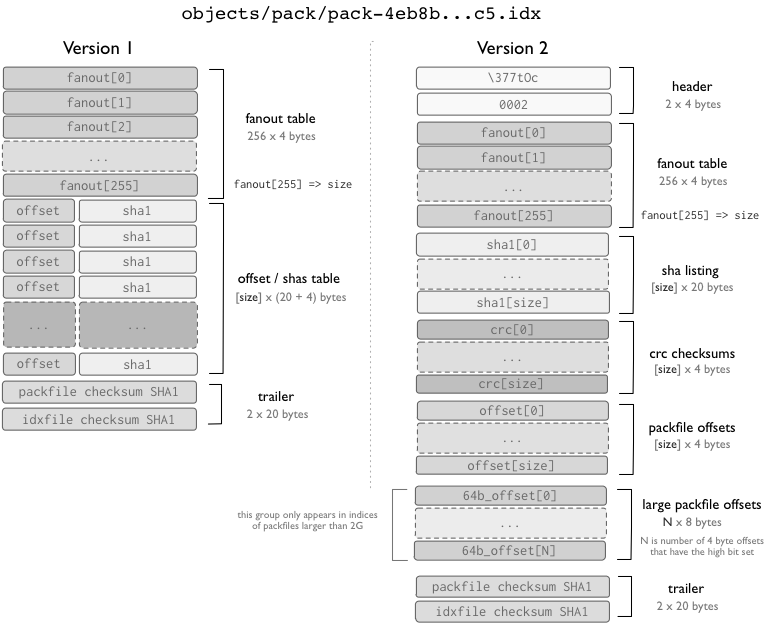
\includegraphics[width=0.80\textwidth]{content/git/packfile-index.png}
\label{fig:packfileindex}
\caption{Packfile Intex}
\end{figure*}

In both formats, the fanout table is simply a way to find the offset of a
particular sha faster within the index file. The offset/sha1[] tables are
sorted by sha1[] values (this is to allow binary search of this table), and
fanout[] table points at the offset/sha1[] table in a specific way (so that
part of the latter table that covers all hashes that start with a given byte
can be found to avoid 8 iterations of the binary search).

In version 1, the offsets and shas are in the same space, where in version two,
there are seperate tables for the shas, crc checksums and offsets. At the end
of both files are checksum shas for both the index file and the packfile it
references.

Importantly, packfile indexes are not neccesary to extract objects from a
packfile, they are simply used to quickly retrieve individual objects from a
pack. The packfile format is used in upload-pack and receieve-pack programs
(push and fetch protocols) to transfer objects and there is no index used then
- it can be built after the fact by scanning the packfile.

\subsubsection{The Packfile Format}
The packfile itself is a very simple format. There is a header, a series of
packed objects (each with it's own header and body) and then a checksum
trailer. The first four bytes is the string 'PACK', which is sort of used to
make sure you're getting the start of the packfile correctly. This is followed
by a 4-byte packfile version number and then a 4-byte number of entries in that
file. In Ruby, you might read the header data like this:
\lstset{basicstyle=\scriptsize, numbers=none, captionpos=b, tabsize=4}
\begin{lstlisting}[caption=,language={ruby},
breaklines=true,label=lst:]
def read_pack_header
  sig = @session.recv(4)
  ver = @session.recv(4).unpack("N")[0]
  entries = @session.recv(4).unpack("N")[0]
  [sig, ver, entries]
end
\end{lstlisting}

After that, you get a series of packed objects, in order of their SHAs which
each consist of an object header and object contents. At the end of the
packfile is a 20-byte SHA1 sum of all the shas (in sorted order) in that
packfile. See figure \ref{fig:packfileformat}

\begin{figure*}[tbp]
\centering
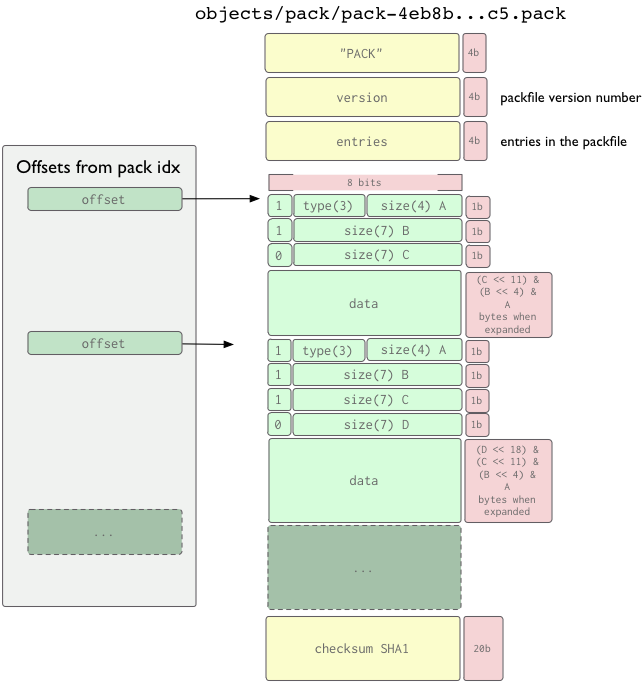
\includegraphics[width=0.80\textwidth]{content/git/packfile-format.png}
\label{fig:packfileformat}
\caption{Packfile format}
\end{figure*}

The object header is a series of one or more 1 byte (8 bit) hunks that specify
the type of object the following data is, and the size of the data when
expanded. Each byte is really 7 bits of data, with the first bit being used to
say if that hunk is the last one or not before the data starts. If the first
bit is a 1, you will read another byte, otherwise the data starts next. The
first 3 bits in the first byte specifies the type of data, according to the
table below.

(Currently, of the 8 values that can be expressed with 3 bits (0-7), 0 (000) is
'undefined' and 5 (101) is not yet used.)

Here, we can see an example of a header of two bytes, where the first specifies
that the following data is a commit, and the remainder of the first and the
last 7 bits of the second specifies that the data will be 144 bytes when
expanded. See figure \ref{fig:packfilelogic}

\begin{figure*}[tbp]
\centering
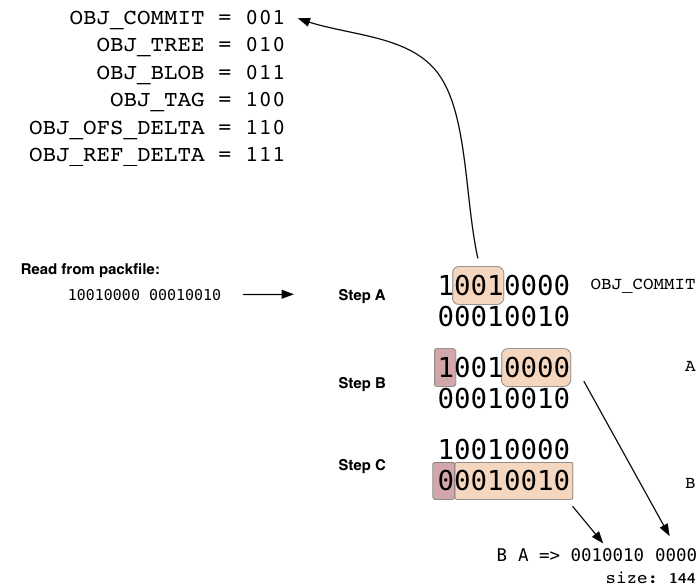
\includegraphics[width=0.80\textwidth]{content/git/packfile-logic.png}
\label{fig:packfilelogic}
\caption{Packfile logic}
\end{figure*}

It is important to note that the size specified in the header data is not the
size of the data that actually follows, but the size of that data when
expanded. This is why the offsets in the packfile index are so useful,
otherwise you have to expand every object just to tell when the next header
starts.

The data part is just zlib stream for non-delta object types; for the two delta
object representations, the data portion contains something that identifies
which base object this delta representation depends on, and the delta to apply
on the base object to resurrect this object.  ref-delta uses 20-byte hash of
the base object at the beginning of data, while ofs-delta stores an offset
within the same packfile to identify the base object. In either case, two
important constraints a reimplementor must adhere to are:

delta representation must be based on some other object within the same
packfile;

the base object must be of the same underlying type (blob, tree, commit or
tag);

\subsection{Raw Git}
Here we will take a look at how to manipulate git at a more raw level, in case
you would like to write a tool that generates new blobs, trees or commits in a
more artificial way. If you want to write a script that uses more low-level git
plumbing to do something new, here are some of the tools you'll need.

\subsubsection{Creating Blobs}
Creating a blob in your Git repository and getting a SHA back is pretty easy.
The git hash-object command is all you'll need. To create a blob object from an
existing file, just run it with the '-w' option (which tells it to write the
blob, not just compute the SHA).
\lstset{basicstyle=\scriptsize, numbers=none, captionpos=b, tabsize=4}
\begin{lstlisting}[caption=,language={bash},
breaklines=true,label=lst:]
$ git hash-object -w myfile.txt
1e4397625791c8ea3bbb5f2279a3

$ git hash-object -w myfile2.txt
ae3185ee32266c860714980dbed7
\end{lstlisting}

The STDOUT output of the command will the the SHA of the blob that was created.

\subsubsection{Creating Trees}
Now lets say you want to create a tree from your new objects. The git mktree
command makes it pretty simple to generate new tree objects from git ls-tree
formatted output. For example, if you write the following to a file named
'/tmp/tree.txt' :
\lstset{basicstyle=\scriptsize, numbers=none, captionpos=b, tabsize=4}
\begin{lstlisting}[caption=,language={bash},
breaklines=true,label=lst:]
100644 blob 1e4397625791c8ea3bbb5f2279a3    file1
100644 blob ae3185ee32266c860714980dbed7    file2
\end{lstlisting}

and then piped that through the git mktree command, Git will write a new tree
to the object database and give you back the new sha of that tree.
\lstset{basicstyle=\scriptsize, numbers=none, captionpos=b, tabsize=4}
\begin{lstlisting}[caption=,language={bash},
breaklines=true,label=lst:]
$ cat /tmp/tree.txt | git mk-tree
fe86d52a66516ace212efa00fe1f
\end{lstlisting}

Then, we can take that and make it a subdirectory of yet another tree, and so
on. If we wanted to create a new tree with that one as a subtree, we just
create a new file (/tmp/newtree.txt) with our new SHA as a tree in it:
\lstset{basicstyle=\scriptsize, numbers=none, captionpos=b, tabsize=4}
\begin{lstlisting}[caption=,language={bash},
breaklines=true,label=lst:]
100644 blob 4664981e4397625791c8ea3bbb5f2279a3    file1-copy
040000 tree ab6a7bfe86d52a66516ace212efa00fe1f    our_files
\end{lstlisting}

and then use git mk-tree again:
\lstset{basicstyle=\scriptsize, numbers=none, captionpos=b, tabsize=4}
\begin{lstlisting}[caption=,language={bash},
breaklines=true,label=lst:]
$ cat /tmp/newtree.txt | git mk-tree
59179bd543a024d6d187692343e2d8ae83
\end{lstlisting}

And we now have an artificial directory structure in Git that looks like this:
\lstset{basicstyle=\scriptsize, numbers=none, captionpos=b, tabsize=4}
\begin{lstlisting}[caption=,language={bash},
breaklines=true,label=lst:]
.
|-- file1-copy
`-- our_files
    |-- file1
    `-- file2

1 directory, 3 files
\end{lstlisting}

without that structure ever having actually existed on disk. Plus, we have a
SHA (5bac6559) that points to it.

\subsubsection{Rearranging Trees}
We can also do tree manipulation by combining trees into new structures using
the index file. As a simple example, let's take the tree we just created and
make a new tree that has two copies of our 5bac6559 tree in it using a
temporary index file. (You can do this by resetting the GIT\_INDEX\_FILE
environment variable or on the command line)

First, we read the tree into our index file under a new prefix using the git
read-tree command, and then write the index contents as a tree using the git
write-tree command:
\lstset{basicstyle=\scriptsize, numbers=none, captionpos=b, tabsize=4}
\begin{lstlisting}[caption=,language={bash},
breaklines=true,label=lst:]
$ export GIT_INDEX_FILE=/tmp/index
$ git read-tree --prefix=copy1/  5bac6559
$ git read-tree --prefix=copy2/  5bac6559
$ git write-tree 
de7625322322382215d9ea78cfe76508c1

$>git ls-tree bb2fa
040000 tree 59179bd543a024d6d187692343e2d8ae83    copy1
040000 tree 59179bd543a024d6d187692343e2d8ae83    copy2
\end{lstlisting}

So now we can see that we've created a new tree just from index manipulation.
You can also do interesting merge operations and such in a temporary index this
way - see the git read-tree docs for more information.

\subsubsection{Creating Commits}
Now that we have a tree SHA, we can create a commit object that points to it.
We can do this using the git commit-tree command. Most of the data that goes
into the commit has to be set as environment variables, so you'll want to set
the following:
\lstset{basicstyle=\scriptsize, numbers=none, captionpos=b, tabsize=4}
\begin{lstlisting}[caption=,language={bash},
breaklines=true,label=lst:]
GIT_AUTHOR_NAME
GIT_AUTHOR_EMAIL
GIT_AUTHOR_DATE
GIT_COMMITTER_NAME
GIT_COMMITTER_EMAIL
GIT_COMMITTER_DATE
\end{lstlisting}

Then you will need to write your commit message to a file or somehow pipe it
into the command through STDIN. Then, you can create your commit object based
on the tree sha we have.
\lstset{basicstyle=\scriptsize, numbers=none, captionpos=b, tabsize=4}
\begin{lstlisting}[caption=,language={bash},
breaklines=true,label=lst:]
$ git commit-tree bb2fa < /tmp/message
a5f85ba5875917319471dfd98dfc636c1dc65650
\end{lstlisting}

If you want to specify one or more parent commits, simply add the shas on the
command line with a '-p' option before each. The SHA of the new commit object
will be returned via STDOUT.

\subsubsection{Updating a Branch Ref}
Now that we have a new commit object SHA, we can update a branch to point to it
if we want to. Lets say we want to update our 'master' branch to point to the
new commit we just created - we would use the git update-ref command:
\lstset{basicstyle=\scriptsize, numbers=none, captionpos=b, tabsize=4}
\begin{lstlisting}[caption=,language={bash},
breaklines=true,label=lst:]
$ git update-ref refs/heads/master a5875917319471dfd98dfc636c1dc65650
\end{lstlisting}

\subsection{Transfer Protocols}
Here we will go over how clients and servers talk to each other to transfer Git
data around.

\subsubsection{Fetching Data over HTTP}
Fetching over an http/s URL will make Git use a slightly dumber protocol. In
this case, all of the logic is entirely on the client side. The server requires
no special setup - any static webserver will work fine if the git directory you
are fetching from is in the webserver path.

In order for this to work, you do need to run a single command on the server
repo everytime anything is updated, though - git update-server-info, which
updates the objects/info/packs and info/refs files to list which refs and
packfiles are available, since you can't do a listing over http. When that
command is run, the objects/info/packs file looks something like this:
\lstset{basicstyle=\scriptsize, numbers=none, captionpos=b, tabsize=4}
\begin{lstlisting}[caption=,language={bash},
breaklines=true,label=lst:]
P pack-ce2bd34abc3d8ebc5922dc81b2e1f30bf17c10cc.pack
P pack-7ad5f5d05f5e20025898c95296fe4b9c861246d8.pack
\end{lstlisting}

So that if the fetch can't find a loose file, it can try these packfiles. The
info/refs file will look something like this:
\lstset{basicstyle=\scriptsize, numbers=none, captionpos=b, tabsize=4}
\begin{lstlisting}[caption=,language={bash},
breaklines=true,label=lst:]
184063c9b594f8968d61a686b2f6052779551613    refs/heads/development
32aae7aef7a412d62192f710f2130302997ec883    refs/heads/master
\end{lstlisting}

Then when you fetch from this repo, it will start with these refs and walk the
commit objects until the client has all the objects that it needs.

For instance, if you ask to fetch the master branch, it will see that master is
pointing to 32aae7ae and that your master is pointing to ab04d88, so you need
32aae7ae. You fetch that object
\lstset{basicstyle=\scriptsize, numbers=none, captionpos=b, tabsize=4}
\begin{lstlisting}[caption=,language={bash},
breaklines=true,label=lst:]
CONNECT http://myserver.com
GET /git/myproject.git/objects/32/aae7aef7a412d62192f710f2130302997ec883 - 200
\end{lstlisting}

and it looks like this:
\lstset{basicstyle=\scriptsize, numbers=none, captionpos=b, tabsize=4}
\begin{lstlisting}[caption=,language={bash},
breaklines=true,label=lst:]
tree aa176fb83a47d00386be237b450fb9dfb5be251a
parent bd71cad2d597d0f1827d4a3f67bb96a646f02889
author Scott Chacon <schacon@gmail.com> 1220463037 -0700
committer Scott Chacon <schacon@gmail.com> 1220463037 -0700

added chapters on private repo setup, scm migration, raw git
\end{lstlisting}

So now it fetches the tree aa176fb8:
\lstset{basicstyle=\scriptsize, numbers=none, captionpos=b, tabsize=4}
\begin{lstlisting}[caption=,language={bash},
breaklines=true,label=lst:]
GET /git/myproject.git/objects/aa/176fb83a47d00386be237b450fb9dfb5be251a - 200
\end{lstlisting}

which looks like this:
\lstset{basicstyle=\scriptsize, numbers=none, captionpos=b, tabsize=4}
\begin{lstlisting}[caption=,language={bash},
breaklines=true,label=lst:]
100644 blob 6ff87c4664981e4397625791c8ea3bbb5f2279a3    COPYING
100644 blob 97b51a6d3685b093cfb345c9e79516e5099a13fb    README
100644 blob 9d1b23b8660817e4a74006f15fae86e2a508c573    Rakefile
\end{lstlisting}

So then it fetches those objects:
\lstset{basicstyle=\scriptsize, numbers=none, captionpos=b, tabsize=4}
\begin{lstlisting}[caption=,language={bash},
breaklines=true,label=lst:]
GET /git/myproject.git/objects/6f/f87c4664981e4397625791c8ea3bbb5f2279a3 - 200
GET /git/myproject.git/objects/97/b51a6d3685b093cfb345c9e79516e5099a13fb - 200
GET /git/myproject.git/objects/9d/1b23b8660817e4a74006f15fae86e2a508c573 - 200
\end{lstlisting}

It actually does this with Curl, and can open up multiple parallel threads to
speed up this process. When it's done recursing the tree pointed to by the
commit, it fetches the next parent.
\lstset{basicstyle=\scriptsize, numbers=none, captionpos=b, tabsize=4}
\begin{lstlisting}[caption=,language={bash},
breaklines=true,label=lst:]
GET /git/myproject.git/objects/bd/71cad2d597d0f1827d4a3f67bb96a646f02889 - 200
\end{lstlisting}

Now in this case, the commit that comes back looks like this:
\lstset{basicstyle=\scriptsize, numbers=none, captionpos=b, tabsize=4}
\begin{lstlisting}[caption=,language={bash},
breaklines=true,label=lst:]
tree b4cc00cf8546edd4fcf29defc3aec14de53e6cf8
parent ab04d884140f7b0cf8bbf86d6883869f16a46f65
author Scott Chacon <schacon@gmail.com> 1220421161 -0700
committer Scott Chacon <schacon@gmail.com> 1220421161 -0700

added chapters on the packfile and how git stores objects
\end{lstlisting}

and we can see that the parent, ab04d88 is where our master branch is currently
pointing. So, we recursively fetch this tree and then stop, since we know we
have everything before this point. You can force Git to double check that we
have everything with the '--recover' option. See git http-fetch for more
information.

If one of the loose object fetches fails, Git will download the packfile
indexes looking for the sha that it needs, then download that packfile.

It is important if you are running a git server that serves repos this way to
implement a post-receive hook that runs the 'git update-server-info' command
each time or there will be confusion. 

\subsubsection{Fetching Data with Upload Pack}
For the smarter protocols, fetching objects is much more efficient. A socket is
opened, either over ssh or over port 9418 (in the case of the git:// protocol),
and the git fetch-pack command on the client begins communicating with a forked
git upload-pack process on the server.

Then the server will tell the client which SHAs it has for each ref, and the
client figures out what it needs and responds with a list of SHAs it wants and
already has.

At this point, the server will generate a packfile with all the objects that
the client needs and begin streaming it down to the client.

Let's look at an example.

The client connects and sends the request header. The clone command
\lstset{basicstyle=\scriptsize, numbers=none, captionpos=b, tabsize=4}
\begin{lstlisting}[caption=,language={bash},
breaklines=true,label=lst:]
$ git clone git://myserver.com/project.git
\end{lstlisting}

produces the following request:
\lstset{basicstyle=\scriptsize, numbers=none, captionpos=b, tabsize=4}
\begin{lstlisting}[caption=,language={bash},
breaklines=true,label=lst:]
0032git-upload-pack /project.git\000host=myserver.com\000
\end{lstlisting}

The first four bytes contain the hex length of the line (including 4 byte line
length and trailing newline if present). Following are the command and
arguments. This is followed by a null byte and then the host information. The
request is terminated by a null byte.

The request is processed and turned into a call to git-upload-pack:
\lstset{basicstyle=\scriptsize, numbers=none, captionpos=b, tabsize=4}
\begin{lstlisting}[caption=,language={bash},
breaklines=true,label=lst:]
$ git-upload-pack /path/to/repos/project.git
\end{lstlisting}

This immediately returns information of the repo:
\lstset{basicstyle=\scriptsize, numbers=none, captionpos=b, tabsize=4}
\begin{lstlisting}[caption=,language={bash},
breaklines=true,label=lst:]
007c74730d410fcb6603ace96f1dc55ea6196122532d HEAD\000multi_ack thin-pack side-band side-band-64k ofs-delta shallow no-progress
003e7d1665144a3a975c05f1f43902ddaf084e784dbe refs/heads/debug
003d5a3f6be755bbb7deae50065988cbfa1ffa9ab68a refs/heads/dist
003e7e47fe2bd8d01d481f44d7af0531bd93d3b21c01 refs/heads/local
003f74730d410fcb6603ace96f1dc55ea6196122532d refs/heads/master
0000
\end{lstlisting}

Each line starts with a four byte line length declaration in hex. The section
is terminated by a line length declaration of 0000.

This is sent back to the client verbatim. The client responds with another
request:
\lstset{basicstyle=\scriptsize, numbers=none, captionpos=b, tabsize=4}
\begin{lstlisting}[caption=,language={bash},
breaklines=true,label=lst:]
0054want 410fcb6603ace96f1dc55ea6196122532d multi_ack side-band-64k ofs-delta
0032want 144a3a975c05f1f43902ddaf084e784dbe
0032want e755bbb7deae50065988cbfa1ffa9ab68a
0032want 2bd8d01d481f44d7af0531bd93d3b21c01
0032want 410fcb6603ace96f1dc55ea6196122532d
00000009done
\end{lstlisting}

The is sent to the open git-upload-pack process which then streams out the
final response:
\lstset{basicstyle=\scriptsize, numbers=none, captionpos=b, tabsize=4}
\begin{lstlisting}[caption=,language={bash},
breaklines=true,label=lst:]
"0008NAK\n"
"0023\002Counting objects: 2797, done.\n"
"002b\002Compressing objects:   0% (1/1177)   \r"
"002c\002Compressing objects:   1% (12/1177)   \r"
"002c\002Compressing objects:   2% (24/1177)   \r"
"002c\002Compressing objects:   3% (36/1177)   \r"
"002c\002Compressing objects:   4% (48/1177)   \r"
"002c\002Compressing objects:   5% (59/1177)   \r"
"002c\002Compressing objects:   6% (71/1177)   \r"
"0053\002Compressing objects:   7% (83/1177)   \rCompressing objects:   8% (95/1177)   \r"
...
"005b\002Compressing objects: 100% (1177/1177)   \rCompressing objects: 100% (1177/1177), done.\n"
"2004\001PACK\000\000\000\002\000\000\n\355\225\017x\234\235\216K\n\302"...
"2005\001\360\204{\225\376\330\345]z2673"...
...
"0037\002Total 2797 (delta 1799), reused 2360 (delta 1529)\n"
...
"<\276\255L\273s\005\001w0006\001[0000"
\end{lstlisting}

See the Packfile chapter previously for the actual format of the packfile data
in the response.

\subsubsection{Pushing Data}
Pushing data over the git and ssh protocols is similar, but simpler. Basically
what happens is the client requests a receive-pack instance, which is started
up if the client has access, then the server returns all the ref head shas it
has again and the client generates a packfile of everything the server needs
(generally only if what is on the server is a direct ancestor of what it is
pushing) and sends that packfile upstream, where the server either stores it on
disk and builds an index for it, or unpacks it (if there aren't many objects in
it)

This entire process is accomplished through the git send-pack command on the
client, which is invoked by git push and the git receive-pack command on the
server side, which is invoked by the ssh connect process or git daemon (if it's
an open push server).


\chapter{Regular Expression}

\chapter{BASH}
\section{Basics}
Some basic bash-script primitives.
\subsection{List directories}
\lstset{basicstyle=\scriptsize, numbers=left, captionpos=b, tabsize=4}
\begin{lstlisting}[caption=Build and Link,language={Bash},
xleftmargin=20pt, label=lst:firstNamsProgram]
#!/bin/bash

Dirlist=$(find . -type d)
for direc in $Dirlist; 
do
	ls $direc
done
\end{lstlisting}

\section{Scripts}
In this section many useful scripts for daily use will be presented. Every
script will have a small piece of documentation.

\subsection{ASM Scripts}
Scripts that help develop assembler programs.

\subsubsection{Build and Link}
\lstset{basicstyle=\scriptsize, numbers=left, captionpos=b, tabsize=4}
\begin{lstlisting}[caption=Build and Link,language={Bash},
xleftmargin=20pt, label=lst:firstNamsProgram]
#/bin/bash

if [ ! -f $1 ]
then
	echo "file doesn't exists"
	exit
fi

fn=$1
l=${#fn}
l4=$(($l-4))
jn=${fn:${l4}:l}
if [ ! .asm == $jn ] 
then
	echo "fail doesn't end on asm"
	exit
fi

if [ `uname -m` == x86_64 ] 
then
	elfType="elf64"
else
	elfType="elf32"
fi

if [ ! $1 == "-g" ]
then
	debug="-g"
else
	debug=""
fi

nasm -f $elfType ${debug} $1
ld -o ${fn:0:${l4}} ${fn:0:${l4}}.o 
\end{lstlisting}
This script allows you to compile and link an asm file with one call. All you
need to do is pass the filename. The filename must have an .asm at it's end.
If you need debug symbols you can pass another args called -g.



\part{Programming Languages}
\chapter{Latex}

\chapter{C Programming Language}
\section{History}
The field of computing as we know it today started in 1947 with three
scientists at Bell Telephone Laboratories--William Shockley, Walter Brattain,
and John Bardeen--and their groundbreaking invention of the transistor. In
1956, the first fully transistor-based computer, the TX-0, was completed at
MIT. The first integrated circuit was created in 1958 by Jack Kilby at Texas
Instruments but, the first high-level programming language existed even before
then.

In 1954, The Fortran project, named for it being the Formula Translator, began.
Fortran begot Algol 58, the Algorithmic Language, in 1958. Algol 58 begot Algol
60 in 1960. Algol 60 begot CPL, the Combined Programming Language, in 1963. CPL
begot BCPL, Basic CPL, in 1967. BCPL begot B in 1969. B begot C in 1971.

B was the first language in the C lineage directly. It was created by Ken
Thompson at Bell Labs and was an interpreted language used in early internal
versions of the UNIX operating system.  Thompson and Dennis Ritchie, also of
Bell Labs, improved B and called it NB. Further extensions to NB created its
logical successor, C, a compiled language. Most of UNIX was then rewritten in
NB and then C, which led to a more portable operating system.

The portability of UNIX was the main reason for the initial popularity of both
UNIX and C. Rather than creating a new operating system for each new machine,
system programmers could simply write the few system-dependent parts required
for the machine, and write a C compiler for the new system. Since most of the
system utilities were therefore written in C, it simply made sense to also
write new utilities in that language.

The American National Standards Institute started work on standardizing the C
language in 1983, and completed the standard in 1989. The standard, ANSI
X3.159-1989 ``Programming Language C'', served as a basis for all
implementations of C compilers. The standards were later updated in 1990 and
1999, allowing for features that were either in common use, or were appearing
in C++. 

\section{A taste of C}
As with nearly every other programming language learning book, we use the
\emph{Hello world} program to introduce you to C.

\lstset{basicstyle=\scriptsize, numbers=left, captionpos=b, tabsize=4}
\begin{lstlisting}[caption=,language={C},
breaklines=true,xleftmargin=15pt,label=lst:]
#include <stdio.h>

int main(void) {
   printf("Hello, world!\n");
   return 0;
}
\end{lstlisting}

This program prints Hello, world! and then exits.
Enter this code into your text editor or IDE, and save it as hello.c.

Then, presuming you are using GCC, type \texttt{gcc -o hello hello.c}. This
tells gcc to compile your hello.c program into a form the machine can execute.
The '-o hello' tells it to call the compiled program 'hello'.

If you have entered this correctly, you should now see a file called hello.
This file is the binary version of your program, and when run should display
Hello, world!

Here is an example of how compiling and running looks when using a terminal on
a unix system. \texttt{ls} is a common unix command that will list the files in
the current directory, which in this case is the directory \texttt{progs}
inside the home directory (represented with the special tilde, \~{}, symbol).
After running the \texttt{gcc} command, \texttt{ls} will list a new file,
\texttt{hello} in green. Green is the standard color coding of \texttt{ls} for
executable files. 

\begin{verbatim}
~/progs$ ls
hello.c
~/progs$ gcc -o hello hello.c
~/progs$ ls
hello  hello.c
~/progs$ ./hello
Hello, world!
~/progs$
\end{verbatim}

\subsection{Part-by-part explanation}
\texttt{\#include \textless{}stdio.h\textgreater{}} tells the C compiler to
find the standard header called \emph{\textless{stdio.h\textgreater{}}} and add
it to this program. In C, you often have to pull in extra optional components
when you need them. \emph{\textless{}stdio.h\textgreater{}} contains
descriptions of standard input/output functions which you can use to send
messages to a user, or to read input from a user.

\texttt{int main(void)} is something you'll find in every C program. Every
program has a \emph{main} function. Generally, the main function is where a
program begins. However, one C program can be scattered across multiple files,
so you won't always find a main function in every file.
The \emph{int} at the beginning means that main will return an integer to the
operating system when it is finished.

\texttt{printf("Hello, world!\textbackslash{}n");} is the statement that
actually puts the message to the screen. \emph{printf} is the formatted
printing function that is declared in the file \emph{stdio.h} --- which is why
you had to \emph{\#include} that at the start of the program.
\emph{\textbackslash{}n} is an escape sequence which adds a new line at the end
of the printed text.

\texttt{return 0;} will return zero (which is the integer referred to on line
3) to the operating system. When a program runs successfully its return value
is zero (GCC4 complains if it doesn't when compiling). A non-zero value is
returned to indicate a warning or error.

The empty line is there because it is (at least on UNIX) considered good
practice to end a file with a new line. In gcc using the \texttt{-Wall
-pedantic -ansi} options, if the file does not end with a new line this message
is displayed: ``warning: no newline at end of file''. (The newline isn't shown
on the example because MediaWiki automatically removes it)

\section{Compiling}
Having covered the basic concepts of C programming, we can now briefly discuss
the process of \emph{compilation}.

Like any programming language, C by itself is completely incomprehensible to a
microprocessor. Its purpose is to provide an intuitive way for humans to
provide instructions that can be easily converted into machine code that
\emph{is} comprehensible to a microprocessor. The \textbf{\emph{compiler}} is
what takes this code, and translates it into the machine code. 

To those new to programming, this seems fairly simple. A naive compiler might
read in every source file, translate everything into machine code, and write
out an executable. This could work, but has two serious problems. First, for a
large project, the computer may not have enough memory to read all of the
source code at once. Second, if you make a change to a single source file, you
would rather not have to recompile the \emph{entire} application. 

To deal with these problems, compilers break their job down into steps; for
each source file (each \texttt{.c} file), the compiler reads the file, reads
the files it references with \texttt{\#include}, and translates it to machine
code. The result of this is an ``object file'' (\texttt{.o}). Once every object
file is made, a ``linker'' collects all of the object files and writes the
actual program. This way, if you change one source file, only that file needs
to be recompiled and then the application needs to be re-linked. 

Without going into the painful details, it can be beneficial to have a
superficial understanding of the compilation process. In brief, here it is: 

\subsection{Preprocessor}
Many times you will need to give special instructions to your compiler. This is
done by inserting \textbf{preprocessor directives} into your code. When you
begin compiling your code, a special program called the preprocessor scans the
source code and preforms simple substitution of tokenized strings for others
according to predefined rules. The preprocessor is not a part of the C
language.

In C language, all preprocessor directives begin with the pound character (\#).
You can see one preprocessor directive in the Hello world program introduced in
A taste of C:

\begin{verbatim}
	#include <stdio.h>
\end{verbatim}

This directive causes the header to be included into your program. Other
directives such as \texttt{\#pragma} control compiler settings and macros. The
result of the preprocessing stage is a text string. You can think of the
preprocessor as a non-interactive text editor that prepares your code for the
compilation step.

\subsection{Syntax Checking}
This step ensures that the code is valid and will sequence into an executable
program. Under some compilers, you may get messages or warnings indicating
potential issues with your program (such as a statement always being true or
false, etc.) 

When an error is detected in the program, the compiler will normally report the
filename and line that is giving trouble. 

\subsection{Object Code}
The compiler produces a machine code equivalent of the source code that can
then be linked into the final program. The code itself can't be executed yet,
as it has to complete the linking stage. 

It's important to note after discussing the basics that compilation is a ``one
way street''. That is, compiling a C source file into machine code is easy, but
``decompiling'' (turning machine code into the C source that creates it) is
not. Decompilers for C do exist, but they rarely create useful code.

\subsection{Linking}
Linking combines the separate object codes into one complete program by
integrating libraries and the code and producing either an executable program
or a library. Linking is performed by a linker, which is often part of a
compiler.

Common errors during this stage are either missing functions, or duplicate
functions.

\subsection{Automation}
For large C projects, many programmers choose to automate compilation, both in
order to reduce user interaction requirements and to speed up the process by
only recompiling modified files.

Most integrated development environments have some kind of project management,
which makes such automation very easy. On UNIX-like systems, make and Makefiles
are often used to accomplish the same.

\section{Variables}
\newcounter{varcnt}
Like most programming languages, C is able to use and process named variables
and their contents. \textbf{Variables} are simply names used to refer to some
location in memory --- a location that holds a value with which we are working. 

It may help to think of variables as a placeholder for a value. You can think
of a variable as being equivalent to its assigned value. So, if you have a
variable \emph{i} that is initialized (set equal) to 4, then it follows that
\emph{i+1} will equal \emph{5}.

Since C is a relatively low-level programming language, before a C program can
utilize memory to store a variable it must claim the memory needed to store the
values for a variable. This is done by \textbf{declaring} variables. Declaring
variables is the way in which a C program shows the number of variables it
needs, what they are going to be named, and how much memory they will need.

Within the C programming language, when managing and working with variables, it
is important to know the \emph{type} of variables and the \emph{size} of these
types. Since C is a fairly low-level programming language, these aspects of its
working can be hardware specific --- that is, how the language is made to work
on one type of machine can be different from how it is made to work on another.

\textbf{All} variables in C are ``typed''. That is, every variable declared
must be assigned as a certain type of variable.

\subsection{Declaring, Initializing, and Assigning Variables}
Here is an example of declaring an integer, which we've called
\texttt{some\_number}. (Note the semicolon at the end of the line; that is how
your compiler separates one program \emph{statement} from another.)
\lstset{basicstyle=\scriptsize, numbers=left, captionpos=b, tabsize=4}
\begin{lstlisting}[caption=Section \thesection listing \arabic{varcnt},language={C},
breaklines=true,xleftmargin=15pt,label=lst:section\thesection listing\arabic{varcnt}]
int some_number;
\end{lstlisting}

This statement means we're declaring some space for a variable called
some\_number, which will be used to store \texttt{int}eger data. Note that we
must specify the type of data that a variable will store. There are specific
keywords to do this --- we'll look at them in the next section.

Multiple variables can be declared with one statement, like this:
\lstset{basicstyle=\scriptsize, numbers=left, captionpos=b, tabsize=4}
\begin{lstlisting}[caption=Section \thesection listing \arabic{varcnt},language={C},
breaklines=true,xleftmargin=15pt,label=lst:section\thesection listing\arabic{varcnt}]
int anumber, anothernumber, yetanothernumber;
\end{lstlisting}
\stepcounter{varcnt}

We can also declare \emph{and} assign some content to a variable at the same time.
\lstset{basicstyle=\scriptsize, numbers=left, captionpos=b, tabsize=4}
\begin{lstlisting}[caption=Section \thesection listing \arabic{varcnt},language={C},
breaklines=true,xleftmargin=15pt,label=lst:section\thesection listing\arabic{varcnt}]
int some_number=3;
\end{lstlisting}
\stepcounter{varcnt}

This is called \emph{initialization}.

In early versions of C, variables must be declared at the beginning of a block.
In C99 it is allowed to mix declarations and statements arbitrarily—but doing
so is not usual, because it is rarely necessary, some compilers still don’t
support C99 (portability), and it may, because it is uncommon yet, irritate
fellow programmers (maintainability).

After declaring variables, you can assign a value to a variable later on using a statement like this:
\lstset{basicstyle=\scriptsize, numbers=left, captionpos=b, tabsize=4}
\begin{lstlisting}[caption=Section \thesection listing \arabic{varcnt},language={C},
breaklines=true,xleftmargin=15pt,label=lst:section\thesection listing\arabic{varcnt}]
some_number=3;
\end{lstlisting}
\stepcounter{varcnt}

You can also assign a variable the value of another variable, like so:
\lstset{basicstyle=\scriptsize, numbers=left, captionpos=b, tabsize=4}
\begin{lstlisting}[caption=Section \thesection listing \arabic{varcnt},language={C},
breaklines=true,xleftmargin=15pt,label=lst:section\thesection listing\arabic{varcnt}]
anumber = anothernumber;
\end{lstlisting}
\stepcounter{varcnt}

Or assign multiple variables the same value with one statement:
\lstset{basicstyle=\scriptsize, numbers=left, captionpos=b, tabsize=4}
\begin{lstlisting}[caption=Section \thesection listing \arabic{varcnt},language={C},
breaklines=true,xleftmargin=15pt,label=lst:section\thesection listing\arabic{varcnt}]
anumber = anothernumber = yetanothernumber = 3;
\end{lstlisting}
\stepcounter{varcnt}

This is because the assignment \texttt{x = y} returns the value of the
assignment. \texttt{x = y = z} is really shorthand for \texttt{x = (y = z)}.

\subsubsection{Naming Variables}
Variable names in C are made up of letters (upper and lower case) and digits.
The underscore character (``\_'') is also permitted. Names must not begin with
a digit. Unlike some languages (such as Perl and some BASIC dialects), C does
not use any special prefix characters on variable names.

Some examples of valid (but not very descriptive) C variable names:
\lstset{basicstyle=\scriptsize, numbers=left, captionpos=b, tabsize=4}
\begin{lstlisting}[caption=Section \thesection listing \arabic{varcnt},language={C},
breaklines=true,xleftmargin=15pt,label=lst:section\thesection listing\arabic{varcnt}]
foo
Bar
BAZ
foo_bar
_foo42
_
QuUx
\end{lstlisting}
\stepcounter{varcnt}

Some examples of invalid C variable names:
\lstset{basicstyle=\scriptsize, numbers=left, captionpos=b, tabsize=4}
\begin{lstlisting}[caption=Section \thesection listing \arabic{varcnt},language={C},
breaklines=true,xleftmargin=15pt,label=lst:section\thesection listing\arabic{varcnt}]
2foo (must not begin with a digit)
my foo (spaces not allowed in names)
$foo ($ not allowed -- only letters, digits, and _)
while (language keywords cannot be used as names)
\end{lstlisting}
\stepcounter{varcnt}

As the last example suggests, certain words are reserved as keywords in the
language, and these cannot be used as variable names.

In addition there are certain sets of names that, while not language keywords,
are reserved for one reason or another. For example, a C compiler might use
certain names ``behind the scenes'', and this might cause problems for a
program that attempts to use them. Also, some names are reserved for possible
future use in the C standard library. The rules for determining exactly what
names are reserved (and in what contexts they are reserved) are too complicated
to describe here, and as a beginner you don't need to worry about them much
anyway. For now, just avoid using names that begin with an underscore
character.

The naming rules for C variables also apply to naming other language constructs
such as function names, struct tags, and macros, all of which will be covered
later.

\subsection{Literals}
Anytime within a program in which you specify a value explicitly instead of
referring to a variable or some other form of data, that value is referred to
as a \textbf{literal}. In the initialization example above, 3 is a literal.
Literals can either take a form defined by their type (more on that soon), or
one can use hexadecimal (hex) notation to directly insert data into a variable
regardless of its type
. Hex numbers are always preceded with \emph{0x}. For now, though, you probably
shouldn't be too concerned with hex.

\subsection{The Four Basic Types}
In Standard C there are four basic data types. They are \texttt{int},
\texttt{char}, \texttt{float}, and \texttt{double}.

We will briefly describe them here, then go into more detail in C
Programming/Types.

\subsubsection{The \texttt{int} type}
The \texttt{int} type stores integers in the form of ``whole numbers''. An
integer is typically the size of one machine word, which on most modern home
PCs is 32 bits (4 octets). Examples of literals are whole numbers (integers)
such as 1,2,3, 10, 100... When \texttt{int} is 32 bits (4 octets), it can store
any whole number (integer) between -2147483648 and 2147483647. A 32 bit word
(number) has the possibility of representing any one number out of 4294967296
possibilities (2 to the power of 32).

If you want to declare a new int variable, use the \texttt{int} keyword. For
example:

\lstset{basicstyle=\scriptsize, numbers=left, captionpos=b, tabsize=4}
\begin{lstlisting}[caption=Section \thesection listing \arabic{varcnt},language={C},
breaklines=true,xleftmargin=15pt,label=lst:section\thesection listing\arabic{varcnt}]
int numberOfStudents, i, j=5;
\end{lstlisting}
\stepcounter{varcnt}

In this declaration we declare 3 variables, numberOfStudents, i and j, j here
is assigned the literal 5.

\subsubsection{The \texttt{char} type}
The \texttt{char} type is capable of holding any member of the execution
character set. It stores the same kind of data as an \texttt{int} (i.e.
integers), but always has a size of one byte. The size of a byte is specified
by the macro \texttt{CHAR\_BIT} which specifies the number of bits in a char
(byte). In standard C it never can be less than 8 bits. A variable of type
\texttt{char} is most often used to store character data, hence its name. Most
implementations use the ASCII character set as the execution character set, but
it's best not to know or care about that unless the actual values are
important.

Examples of character literals are a, b, 1, etc., as well as some special
characters such as \texttt{\textbackslash{}0} (the null character) and
\texttt{\textbackslash{}n} (newline, recall Hello, World). Note that the
\texttt{char} value must be enclosed within single quotations.

When we initialize a character variable, we can do it two ways. One is
preferred, the other way is \textbf{\emph{bad}} programming practice.

The first way is to write
\lstset{basicstyle=\scriptsize, numbers=left, captionpos=b, tabsize=4}
\begin{lstlisting}[caption=Section \thesection listing \arabic{varcnt},language={C},
breaklines=true,xleftmargin=15pt,label=lst:section\thesection listing\arabic{varcnt}]
char letter1 = 'a';
\end{lstlisting}
\stepcounter{varcnt}

This is \emph{good} programming practice in that it allows a person reading
your code to understand that letter1 is being initialized with the letter 'a'
to start off with.

The second way, which should \emph{not} be used when you are coding letter
characters, is to write
\lstset{basicstyle=\scriptsize, numbers=left, captionpos=b, tabsize=4}
\begin{lstlisting}[caption=Section \thesection listing \arabic{varcnt},language={C},
breaklines=true,xleftmargin=15pt,label=lst:section\thesection listing\arabic{varcnt}]
char letter2 = 97; /* in ASCII, 97 = 'a' */
\end{lstlisting}
\stepcounter{varcnt}

This is considered by some to be extremely \textbf{\emph{bad}} practice, if we
are using it to store a character, not a small number, in that if someone reads
your code, most readers are forced to look up what character corresponds with
the number 97 in the encoding scheme. In the end, \texttt{letter1} and
\texttt{letter2} store both the same thing -- the letter a, but the first
method is clearer, easier to debug, and much more straightforward. 

One important thing to mention is that characters for numerals are represented
differently from their corresponding number, i.e.\ '1' is not equal to 1. 

There is one more kind of literal that needs to be explained in connection with
chars: the \textbf{string literal}. A string is a series of characters, usually
intended to be displayed. They are surrounded by double quotations (`` '', not
' '). An example of a string literal is the ``Hello, world!\textbackslash{}n''
in the \"Hello, World\" example.

\subsubsection{The \texttt{float} type}
\texttt{float} is short for Floating Point. It stores real numbers also, but is
only one machine word in size. Therefore, it is used when less precision than a
double provides is required. \texttt{float} literals must be suffixed with F or
f, otherwise they will be interpreted as doubles. Examples are: 3.1415926f,
4.0f, 6.022e+23f. float variables can be declared using the \texttt{float}
keyword.

\subsubsection{The \texttt{double} type}
The \texttt{double} and \texttt{float} types are very similar. The
\texttt{float} type allows you to store single-precision floating point
numbers, while the \texttt{double} keyword allows you to store double-precision
floating point numbers --- real numbers, in other words, both integer and
non-integer values. Its size is typically two machine words, or 8 bytes on most
machines. Examples of \texttt{double} literals are 3.1415926535897932, 4.0,
6.022e+23 (\href{http://en.wikipedia.org/wiki/Scientific\_notation}{scientific
notation}). If you use 4 instead of 4.0, the 4 will be interpreted as an
\texttt{int}.

The distinction between floats and doubles was made because of the differing
sizes of the two types. When C was first used, space was at a minimum and so
the judicious use of a float instead of a double saved some memory. Nowadays,
with memory more freely available, you do not really need to conserve memory
like this --- it may be better to use doubles consistently. Indeed, some C
implementations use doubles instead of floats when you declare a float
variable.

If you want to use a double variable, use the \texttt{double} keyword.

\subsection{\texttt{sizeof}}
If you have any doubts as to the amount of memory actually used by any type
(and this goes for types we'll discuss later, also), you can use the
\texttt{sizeof} operator to find out for sure. (For completeness, it is
important to mention that \texttt{sizeof} is a compile-time unary operator, not
a function.) Its syntax is:

\lstset{basicstyle=\scriptsize, numbers=left, captionpos=b, tabsize=4}
\begin{lstlisting}[caption=Section \thesection listing \arabic{varcnt},language={C},
breaklines=true,xleftmargin=15pt,label=lst:section\thesection listing\arabic{varcnt}]
sizeof object
sizeof(type)
\end{lstlisting}
\stepcounter{varcnt}

The two expressions above return the size of the object and type specified, in
bytes. The return type is \texttt{size\_t} (defined in the header
\texttt{\textless{}stddef.h\textgreater{}}) which is an unsigned value. Here's
an example usage:

\lstset{basicstyle=\scriptsize, numbers=left, captionpos=b, tabsize=4}
\begin{lstlisting}[caption=Section \thesection listing \arabic{varcnt},language={C},
breaklines=true,xleftmargin=15pt,label=lst:section\thesection listing\arabic{varcnt}]
size_t size;
int i;
size = sizeof(i);
\end{lstlisting}
\stepcounter{varcnt}

\texttt{size} will be set to 4, assuming \texttt{CHAR\_BIT} is defined as 8,
and an integer is 32 bits wide. The value of \texttt{sizeof}'s result is the
number of bytes.

Note that when \texttt{sizeof} is applied to a \texttt{char}, the result is 1;
that is:

\lstset{basicstyle=\scriptsize, numbers=left, captionpos=b, tabsize=4}
\begin{lstlisting}[caption=Section \thesection listing \arabic{varcnt},language={C},
breaklines=true,xleftmargin=15pt,label=lst:section\thesection listing\arabic{varcnt}]
sizeof(char)
\end{lstlisting}
\stepcounter{varcnt}

always returns 1.

\subsection{Data type modifiers}
One can alter the data storage of any data type by preceding it with certain
modifiers.

\texttt{long} and \texttt{short} are modifiers that make it possible for a data
type to use either more or less memory. The \texttt{int} keyword need not
follow the \texttt{short} and \texttt{long} keywords. This is most commonly the
case. A \texttt{short} can be used where the values fall within a lesser range
than that of an \texttt{int}, typically -32768 to 32767. A \texttt{long} can be
used to contain an extended range of values. It is not guaranteed that a
\texttt{short} uses less memory than an \texttt{int}, nor is it guaranteed that
a \texttt{long} takes up more memory than an \texttt{int}. It is only
guaranteed that sizeof(short) \textless{}= sizeof(int) \textless{}=
sizeof(long). Typically a \texttt{short} is 2 bytes, an \texttt{int} is 4
bytes, and a \texttt{long} either 4 or 8 bytes. Modern C compilers also provide
\texttt{long long} which is
typically an 8 byte integer. 

In all of the types described above, one bit is used to indicate the sign
(positive or negative) of a value. If you decide that a variable will never
hold a negative value, you may use the \texttt{unsigned} modifier to use that
one bit for storing other data, effectively doubling the range of values while
mandating that those values be positive. The \texttt{unsigned} specifier also
may be used without a trailing \texttt{int}, in which case the size defaults to
that of an \texttt{int}. There is also a \textbf{signed} modifier which is the
opposite, but it is not necessary, except for certain uses of \texttt{char},
and seldom used since all types (except \texttt{char}) are signed by default.

To use a modifier, just declare a variable with the data type and relevant modifiers:
\lstset{basicstyle=\scriptsize, numbers=left, captionpos=b, tabsize=4}
\begin{lstlisting}[caption=Section \thesection listing \arabic{varcnt},language={C},
breaklines=true,xleftmargin=15pt,label=lst:section\thesection listing\arabic{varcnt}]
unsigned short int usi; /* fully qualified --- unsigned short int */
short si; /* short int */
unsigned long uli; /* unsigned long int */
\end{lstlisting}
\stepcounter{varcnt}

\subsection{\texttt{const} qualifier}
When the \textbf{const} qualifier is used, the declared variable must be
initialized at declaration. It is then not allowed to be changed.

While the idea of a variable that never changes may not seem useful, there are
good reasons to use \texttt{const}. For one thing, many compilers can perform
some small optimizations on data when it knows that data will never change. For
example, if you need the value of \ensuremath{\pi} in your calculations, you
can declare a const variable of \texttt{pi}, so a program or another function
written by someone else cannot change the value of \texttt{pi}.

Note that a Standard conforming compiler must issue a warning if an attempt is
made to change a \texttt{cons}t variable --- but after doing so the compiler is
free to ignore the \\texttt{onst} qualifier.

\subsection{Magic numbers}
When you write C programs, you may be tempted to write code that will depend on
certain numbers. For example, you may be writing a program for a grocery store.
This complex program has thousands upon thousands of lines of code. The
programmer decides to represent the cost of a can of corn, currently 99 cents,
as a literal throughout the code. Now, assume the cost of a can of corn changes
to 89 cents. The programmer must now go in and manually change each entry of 99
cents to 89. While this is not that big of a problem, considering the ``global
find-replace'' function of many text editors, consider another problem: the
cost of a can of green beans is also initially 99 cents. To reliably change the
price, you have to look at every occurrence of the number 99.

C possesses certain functionality to avoid this. This functionality is
approximately equivalent, though one method can be useful in one circumstance,
over another.

\subsection{Using the \texttt{const} keyword}
The \texttt{const} keyword helps eradicate \textbf{magic numbers}. By declaring
a variable \texttt{const corn} at the beginning of a block, a programmer can
simply change that const and not have to worry about setting the value
elsewhere.

There is also another method for avoiding magic numbers. It is much more
flexible than \texttt{const}, and also much more problematic in many ways. It
also involves the preprocessor, as opposed to the compiler. Behold...

\subsubsection{\#define}
When you write programs, you can create what is known as a \emph{macro}, so
when the computer is reading your code, it will replace all instances of a word
with the specified expression.

Here's an example. If you write
\begin{enumerate}
\setlength{\leftmargin}{0pt}
\setlength{\itemsep}{0pt}
\setlength{\parsep}{0pt}
\setlength{\parskip}{0pt}
	\item define PRICE\_OF\_CORN 0.99
\end{enumerate}

when you want to, for example, print the price of corn, you use the word
\texttt{PRICE\_OF\_CORN} instead of the number 0.99 --- the preprocessor will
replace all instances of \texttt{PRICE\_OF\_CORN} with 0.99, which the compiler
will interpret as the literal \texttt{double} 0.99. The preprocessor performs
substitution, that is, \texttt{PRICE\_OF\_CORN} is replaced by 0.99 so this
means there is no need for a semicolon.

It is important to note that \texttt{\#define} has basically the same
functionality as the ``find-and-replace'' function in a lot of text
editors/word processors. 

For some purposes, \texttt{\#define} can be harmfully used, and it is usually
preferable to use \texttt{const} if \texttt{\#define} is unnecessary. It is
possible, for instance, to \texttt{\#define}, say, a macro \texttt{DOG} as the
number 3, but if you try to print the macro, thinking that \texttt{DOG}
represents a string that you can show on the screen, the program will have an
error. \texttt{\#define} also has no regard for type. It disregards the
structure of your program, replacing the text \emph{everywhere} (in effect,
disregarding scope), which could be advantageous in some circumstances, but can
be the source of problematic bugs.

You will see further instances of the \texttt{\#define} directive later in the
text. It is good convention to write \texttt{\#define}d words in all capitals,
so a programmer will know that this is not a variable that you have declared
but a \texttt{\#define}d macro.

\subsection{Scope}
In the Basic Concepts section, the concept of scope was introduced. It is
important to revisit the distinction between local types and global types, and
how to declare variables of each. To declare a local variable, you place the
declaration at the beginning (i.e. before any non-declarative statements) of
the block to which the variable is intended to be local. To declare a global
variable, declare the variable outside of any block. If a variable is global,
it can be read, and written, from anywhere in your program.

Global variables are not considered good programming practice, and should be
avoided whenever possible. They inhibit code readability, create naming
conflicts, waste memory, and can create difficult-to-trace bugs. Excessive
usage of globals is usually a sign of laziness and/or poor design. However, if
there is a situation where local variables may create more obtuse and
unreadable code, there's no shame in using globals.

\subsection{Other Modifiers}
Included here, for completeness, are more of the modifiers that standard C
provides. For the beginning programmer, \emph{static} and \emph{extern} may be
useful. \emph{volatile} is more of interest to advanced programmers.
\emph{register} and \emph{auto} are largely deprecated and are generally not of
interest to either beginning or advanced programmers.

\textbf{static} is sometimes a useful keyword.  It is a common misbelief that
the only purpose is to make a variable stay in memory. When you declare a
function or global variable as \emph{static} it will become internal. You
cannot access the function or variable through the extern (see below) keyword
from other files in your project. When you declare a local variable as
\emph{static}, it is created just like any other variable. However, when the
variable goes out of scope (i.e. the block it was local to is finished) the
variable stays in memory, retaining its value. The variable stays in memory
until the program ends. While this behaviour resembles that of global
variables, static variables still obey scope rules and therefore cannot be
accessed outside of their scope. Variables declared static are initialized to
zero (or for pointers, NULL) by default. 

You can use static in (at least) two different ways. Consider this code, and
imagine it is in a file called jfile.c:


\lstset{basicstyle=\scriptsize, numbers=left, captionpos=b, tabsize=4}
\begin{lstlisting}[caption=Section \thesection listing \arabic{varcnt},language={C},
breaklines=true,xleftmargin=15pt,label=lst:section\thesection listing\arabic{varcnt}]
include <stdio.h>
static int j = 0;
	
void up(void) {
	/* k is set to 0 when the program starts. The line is then "ignored"
	 * for the rest of the program (i.e. k is not set to 0 every time up()
	 * is called)
	 */
	static int k = 0;
	j++;
	k++;
	printf("up() called.   k= %2d, j= %2d\n", k , j);
}
	
void down(void) {
	static int k = 0;
	j--;
	k--;
	printf("down() called. k= %2d, j= %2d\n", k , j);
}
	
int main(void) {
	int i;
	  
	/* call the up function 3 times, then the down function 2 times */
	for (i= 0; i < 3; i++)
	   up();
	for (i= 0; i < 2; i++)
	   down();
	 
	return 0;
}
\end{lstlisting}
\stepcounter{varcnt}

The j var is accessible by both up and down and retains its value. the k vars
also retain their value, but they are two different variables in each their
scopes. static vars are a good way to implement encapsulation, a term from the
object-oriented way of thinking that effectively means not allowing changes to
be made to a variable except through function calls.

Running the program above will produce the following output:
\lstset{basicstyle=\scriptsize, numbers=left, captionpos=b, tabsize=4}
\begin{lstlisting}[caption=Section \thesection listing \arabic{varcnt},language={C},
breaklines=true,xleftmargin=15pt,label=lst:section\thesection listing\arabic{varcnt}]
up() called. k= 1, j= 1
up() called. k= 2, j= 2
up() called. k= 3, j= 3
down() called. k= -1, j= 2
down() called. k= -2, j= 1
\end{lstlisting}
\stepcounter{varcnt}

\textbf{extern} is used when a file needs to access a variable in another file
that it may not have \textit{\#included} directly.  Therefore, \emph{extern}
does not actually carve out space for a new variable, it just provides the
compiler with sufficient information to access the remote variable.

\textbf{\texttt{volatile}} is a special type modifier which informs the
compiler that the value of the variable may be changed by external entities
other than the program itself. This is necessary for certain programs compiled
with optimizations --- if a variable were not defined \texttt{volatile} then
the compiler may assume that certain operations involving the variable are safe
to optimize away when in fact they aren't. \emph{volatile} is particularly
relevant when working with embedded systems (where a program may not have
complete control of a variable) and multi-threaded applications.

\textbf{auto} is a modifier which specifies an ``automatic'' variable that is
automatically created when in scope and destroyed when out of scope. If you
think this sounds like pretty much what you've been doing all along when you
declare a variable, you're right: all declared items within a block are
implicitly ``automatic''. For this reason, the \emph{auto} keyword is more like
the answer to a trivia question than a useful modifier, and there are lots of
very competent programmers that are unaware of its existence.

\textbf{\texttt{register}} is a hint to the compiler to attempt to optimize the
storage of the given variable by storing it in a register of the computer's CPU
when the program is run. Most optimizing compilers do this anyway, so use of
this keyword is often unnecessary. In fact, ANSI C states that a compiler can
ignore this keyword if it so desires -- and many do. Microsoft Visual C++ is an
example of an implementation that completely ignores the \emph{register}
keyword.

\section{Input and Output}
When you take time to consider it, a computer would be pretty useless without
some way to talk to the people who use it. Just like we need information in
order to accomplish tasks, so do computers. And just as we supply information
to others so that they can do tasks, so do computers.  These supplies and
returns of information to a computer are called input and output. 'Input' is
information supplied to a computer or program. 'Output' is information provided
by a computer or program. Frequently, computer programmers will lump the
discussion in the more general term input/output or simply, I/O.  In C, there
are many different ways for a program to communicate with the user. Amazingly,
the most simple methods usually taught to beginning programmers may also be the
most powerful. In the "Hello, World" example at the beginning of this text, we
were introduced to a Standard Library file stdio.h, and one of its functions,
printf(). Here we discuss more of the functions that stdio.h gives us.

\subsection{Output using printf}
Recall from the beginning of this text the demonstration program duplicated below:
\lstset{basicstyle=\scriptsize, numbers=left, captionpos=b, tabsize=4}
\begin{lstlisting}[caption=,language={C},
breaklines=true,xleftmargin=15pt,label=lst:]
#include <stdio.h>

int main(void) {
	printf("Hello, world!\n");
	return 0;
}
\end{lstlisting}

If you compile and run this program, you will see the sentence below show up on
your screen:

\scriptsize
\begin{verbatim}
Hello, world!
\end{verbatim}
\normalsize

This amazing accomplishment was achieved by using the function printf(). A
function is like a "black box" that does something for you without exposing the
internals inside. We can write functions ourselves in C, but we will cover that
later.  You have seen that to use printf() one puts text, surrounded by quotes,
in between the parentheses. We call the text surrounded by quotes a literal
string (or just a string), and we call that string an argument to printf.  As a
note of explanation, it is sometimes convenient to include the open and closing
parentheses after a function name to remind us that it is, indeed, a function.
However usually when the name of the function we are talking about is
understood, it is not necessary.  As you can see in the example above, using
printf() can be as simple as typing in some text, surrounded by double quotes
(note that these are double quotes and not two single quotes). So, for example,
you can print any string by placing it as an argument to the printf() function:
\lstset{basicstyle=\scriptsize, numbers=left, captionpos=b, tabsize=4}
\begin{lstlisting}[caption=,language={C},
breaklines=true,xleftmargin=15pt,label=lst:]
printf("This sentence will print out exactly as you see it...");
\end{lstlisting}

And once it is contained in a proper main() function, it will show:
\scriptsize
\begin{verbatim}
This sentence will print out exactly as you see it...
\end{verbatim}
\normalsize

\subsection{Printing numbers and escape sequences}
\subsubsection{Placeholder codes}
The printf function is a powerful function, and is probably the most-used
function in C programs.  For example, let us look at a problem. Say we don't
know what 1905 + 31214 is. Let's use C to get the answer.  We start writing
\lstset{basicstyle=\scriptsize, numbers=left, captionpos=b, tabsize=4}
\begin{lstlisting}[caption=,language={C},
breaklines=true,xleftmargin=15pt,label=lst:]
#include <stdio.h> // this is important, since printf 
                   // can't be used without this line
int main(void) {
	printf("1905+31214 is");
}
\end{lstlisting}

but here we are stuck! printf only prints strings! Thankfully, printf has
methods for printing numbers. What we do is put a placeholder format code in
the string. We write:
\scriptsize
\begin{verbatim}
printf("1905+31214 is %d", 1905+31214);
\end{verbatim}
\normalsize

The placeholder \%d literally "holds the place" for the actual number that is
the result of adding 1905 to 31214.  These placeholders are called format
specifiers. Many other format specifiers work with printf. If we have a
floating-point number, we can use \%f to print out a floating-point number,
decimal point and all. Other format specifiers are:
\begin{itemize}
\item \%i - int (same as \%d)
\item \%lf - double
\item \%c - char
\item \%s - string
\item \%x - hexadecimal
\end{itemize}

\subsubsection{Tabs and newlines}
What if, we want to achieve some output that will look like:
\scriptsize
\begin{verbatim}
   1905 
  31214 +
  -----
\end{verbatim}
\normalsize

printf will not put line breaks in at the end of each statement: we must do
this ourselves. But how?  What we can do is use the newline escape character.
An escape character is a special character that we can write but will do
something special onscreen, such as make a beep, write a tab, and so on. To
write a newline we write \\n. All escape characters start with a backslash.  So
to achieve the output above, we write
\lstset{basicstyle=\scriptsize, numbers=left, captionpos=b, tabsize=4}
\begin{lstlisting}[caption=,language={C},
breaklines=true,xleftmargin=15pt,label=lst:]
printf(" 1905\n31214 +\n-----\n");
\end{lstlisting}

or to be a bit more clear, we can break this long printf statement over several
lines. So our program will be
\lstset{basicstyle=\scriptsize, numbers=left, captionpos=b, tabsize=4}
\begin{lstlisting}[caption=,language={C},
breaklines=true,xleftmargin=15pt,label=lst:]
#include <stdio.h>
 
int main(void) {
	printf(" 1905\n");
	printf("31214 +\n");
	printf("-----\n");
	printf("%d", 1905+31214);
	return 0;
}
\end{lstlisting}
There are other escape characters we can use. Another common one is to use \\t
to write a tab. You can use \\a to ring the computer's bell, but you should not
use this very much in your programs, as excessive use of sound is not very
friendly to the user.

\subsection{Other output methods}
\subsubsection{puts()}
The puts() function is a very simple way to send a string to the screen when
you have no placeholders to be concerned about. It works very much like the
printf() function we saw the "Hello, World!" example:
\scriptsize
\begin{verbatim}
puts("Print this string.");
\end{verbatim}
\normalsize

will print to the screen:
\lstset{basicstyle=\scriptsize, numbers=left, captionpos=b, tabsize=4}
\begin{lstlisting}[caption=,language={C},
breaklines=true,xleftmargin=15pt,label=lst:]
Print this string.
\end{lstlisting}

followed by the newline character (as discussed above). (The puts function
appends a newline character to its output.) The fputs function is similar:
\lstset{basicstyle=\scriptsize, numbers=left, captionpos=b, tabsize=4}
\begin{lstlisting}[caption=,language={C},
breaklines=true,xleftmargin=15pt,label=lst:]
fputs("Print this string via fputs", stdout);
\end{lstlisting}

will print to the stdout file (usually the screen):
\scriptsize
\begin{verbatim}
Print this string via fputs
\end{verbatim}
\normalsize

without a newline tacked on to the end.  Since puts() and fputs() does not
allow the placeholders and the associated formatting that printf() allows, for
most programmers learning printf() is sufficient for their needs.

\subsection{Input using scanf()}
The scanf() function is the input method equivalent to the printf() output
function - simple yet powerful. In its simplest invocation, the scanf format
string holds a single placeholder representing the type of value that will be
entered by the user. These placeholders are exactly the same as the printf()
function - \%d for ints, \%f for floats, and \%lf for doubles. There is, however,
one variation to scanf() as compared to printf(). The scanf() function requires
the memory address of the variable to which you want to save the input value.
While pointers are possible here, this is a concept that won't be approached
until later in the text. Instead, the simple technique is to use the address-of
operator, \&. For now it may be best to consider this "magic" before we discuss
pointers. A typical application might be like this:
\lstset{basicstyle=\scriptsize, numbers=left, captionpos=b, tabsize=4}
\begin{lstlisting}[caption=,language={C},
breaklines=true,xleftmargin=15pt,label=lst:]
#include "stdio.h"
 
int main(void) {
	int a;
	
	printf("Please input an integer value: ");
	scanf("%d", &a);
	printf("You entered: %d\n", a);
	
	return 0;
}
\end{lstlisting}

If you were to describe the effect of the scanf() function call above, it might
read as: "Read in an integer from the user and store it at the address of
variable a".  If you are trying to input a string using scanf, you should not
include the \& operator. The code below will not compile.
\lstset{basicstyle=\scriptsize, numbers=left, captionpos=b, tabsize=4}
\begin{lstlisting}[caption=,language={C},
breaklines=true,xleftmargin=15pt,label=lst:]
scanf("%s", &a);
\end{lstlisting}

The correct usage would be:
\lstset{basicstyle=\scriptsize, numbers=left, captionpos=b, tabsize=4}
\begin{lstlisting}[caption=,language={C},
breaklines=true,xleftmargin=15pt,label=lst:]
scanf("%s", a);
\end{lstlisting}
Note of caution on inputs: When data is typed at a keyboard, the information
does not go straight to the program that is running. It is first stored in what
is known as a buffer - a small amount of memory reserved for the input source.
Sometimes there will be data left in the buffer when the program wants to read
from the input source, and the scanf() function will read this data instead of
waiting for the user to type something. Some may suggest you use the function
fflush(stdin), which may work as desired on some computers, but isn't
considered good practice, as you will see later. Doing this has the downfall
that if you take your code to a different computer with a different compiler,
your code may not work properly.

\section{Simple math}
\subsection{Operators and Assignments}
C has a wide range of operators that make simple math easy to handle. The list
of operators grouped into precedence levels is as follows:

\subsubsection{Primary expressions}
An identifier is a primary expression, provided that it has been declared as
designating an object (in which case it is an lvalue value that can be used as
the left side of an assignment expression) or a function (in which case it is a
function designator).

A constant is a primary expression. Its type depends on its form and value.

A string literal is a primary expression.

A parenthesized expression is a primary expression. Its type and value are
those of the unparenthesized expression.

\subsubsection{Postfix operators}
First, a primary expression is also a postfix expression. The following
expressions are also postfix expressions:

A postfix expression followed by a left square bracket (\texttt{[}), an
expression, and a right square bracket (\texttt{]}) constitutes an invocation
of the array subscript operator. One of the expressions shall have type
``pointer to object \emph{type}'' and the other shall have an integer type; the
result type is \emph{type}. Successive array subscript operators designate an
element of a multidimensional array.

A postfix expression followed by parentheses or an optional parenthesized
argument list indicates an invocation of the function call operator.

A postfix expression followed by a dot (\texttt{.}) followed by an identifier
selects a member from a structure or union; a postfix expression followed by an
arrow (\texttt{-\textgreater{}}) followed by an identifier selects a member
from a structure or union who is pointed to by the pointer on the left-hand
side of the expression.

A postfix expression followed by the increment or decrement operators
(\texttt{++} or \texttt{--}) indicates that the variable is to be incremented
or decremented as a side effect. The value of the expression is the value of
the postfix expression \emph{before} the increment or decrement.

\subsubsection{Unary operators}

First, a unary expression is a postfix expression. The following expressions
are all postfix expressions:

The increment or decrement operators followed by a unary expression is a unary
expression. The value of the expression is the value of the unary expression
\emph{after} the increment or decrement.

The following operators followed by a cast expression are unary expressions:
\begin{verbatim}
	Operator     Meaning
	========     =======
	   &         Address-of; value is the 
				 location of the operand
	   *         Contents-of; value is what 
	   *         is stored at the location
	   -         Negation
	   +         Value-of operator
	   !         Logical negation ( (!E) is 
				 equivalent to (0==E) )
	   ~         Bit-wise complement
\end{verbatim}

The keyword \texttt{sizeof} followed by a unary expression is a unary
expression. The value is the size of the type of the expression in bytes. The
expression is not evaluated.

The keyword \texttt{sizeof} followed by a parenthesized type name is a unary
expression. The value is the size of the type in bytes.

\subsubsection{Cast operators}
A cast expression is a unary expression.

A parenthesized type name followed by a cast expression is a cast expression.
The parenthesized type name has the effect of forcing the cast expression into
the type specified by the type name in parentheses. For arithmetic types, this
either does not change the value of the expression, or truncates the value of
the expression if the expression is an integer and the new type is smaller than
the previous type.

\subsubsection{Multiplicative and additive operators}
In C, simple math is very easy to handle. The following operators exist: +
(addition), --- (subtraction), * (multiplication), / (division), and \%
(modulus); You likely know all of them from your math classes --- except,
perhaps, modulus. It returns the \textbf{remainder} of a division (e.g. 5 \% 2
= 1). 

Care must be taken with the modulus, because it's not the equivalent of the
mathematical modulus: (-5) \% 2 is not 1, but -1. Division of integers will
return an integer, and the division of a negative integer by a positive integer
will round towards zero instead of rounding down (e.g. (-5) / 3 = -1 instead of
-2).

There is no inline operator to do the power (e.g. 5 \^{} 2 is \textbf{not} 25,
and 5 ** 2 is an error), but there is a power function.

The mathematical order of operations does apply. For example (2 + 3) * 2 = 10
while 2 + 3 * 2 = 8. The order of precedence in C is BFDMAS: Brackets (or
parentheses), Functions, Division or Multiplication (from left to right,
whichever comes first), Addition or Subtraction (also from left to right,
whichever comes first).

Actually, there are more operators than the above in C.

Assignment in C is simple. You declare the type of variable, the name of the
variable and what it's equal to. For example, int x = 0; double y = 0.0; char z
= 'a';

\lstset{basicstyle=\scriptsize, numbers=left, captionpos=b, tabsize=4}
\begin{lstlisting}[caption=,language={C},
breaklines=true,xleftmargin=15pt,label=lst:]
#include <stdio.h>

int main() {
	int i = 0, j = 0;
	
	/* while i is less than 5 AND j is less than 5, loop */
	while( (i < 5) && (j < 5) ) {
		/* postfix increment, i++
		 *     the value of i is read and then incremented */
		printf("i: %d\t", i++);
		
		/* prefix increment, ++j 
		 *     the value of j is incremented and then read */
		printf("j: %d\n", ++j);
	}
	
	printf("At the end they have both equal values:\ni: %d\tj: %d\n", i, j);
	
	return 0;
}
\end{lstlisting}

will display the following:

\begin{verbatim}
	i: 0    j: 1
	i: 1    j: 2
	i: 2    j: 3
	i: 3    j: 4
	i: 4    j: 5
	At the end they have both equal values:
	i: 5    j: 5
\end{verbatim}

\subsubsection{shift and rotate}
Shift functions are often used in low-level I/O hardware interfacing.  Shift
and rotate functions are heavily used in cryptography and software floating
point emulation.  Other than that, shifts can be used in place of division or
multiplication by a power of two.  Many processors have dedicated function
blocks to make these operations fast -- see Microprocessor Design/Shift and
Rotate Blocks. On processors which have such blocks, most C compilers compile
shift and rotate operators to a single assembly-language instruction -- see X86
Assembly/Shift and Rotate.

\paragraph{shift left}
The \texttt{\textless{}\textless{}} operator shifts the binary representation
to the left, dropping the most significant bits and appending it with zero
bits.  The result is equivalent to multiplying the integer by a power of two.

\paragraph{unsigned shift right}
The unsigned shift right operator, also sometimes called the logical right
shift operator.  It shifts the binary representation to the right, dropping the
least significant bits and prepending it with zeros.  The
\texttt{\textgreater{}\textgreater{}} operator is equivalent to division by a
power of two for unsigned integers.

\paragraph{signed shift right}
The signed shift right operator, also sometimes called the arithmetic right
shift operator.  It shifts the binary representation to the right, dropping the
least significant bit, but prepending it with copies of the original sign bit.
The \texttt{\textgreater{}\textgreater{}} operator is not equivalent to
division for signed integers.

In C, the behavior of the \texttt{\textgreater{}\textgreater{}} operator
depends on the data type it acts on.  Therefore, a signed and an unsigned right
shift looks exactly the same, but produces a different result in some cases.

\paragraph{rotate right}
Contrary to popular belief, it is possible to write C code that compiles down
to the ``rotate'' assembly language instruction (on CPUs that have such an
instruction).

Most compilers recognize this idiom:

\lstset{basicstyle=\scriptsize, numbers=left, captionpos=b, tabsize=4}
\begin{lstlisting}[caption=,language={C},
breaklines=true,xleftmargin=15pt,label=lst:]
	unsigned int x;
	unsigned int y;
	/* ... */
	y = (x >> shift) | (x << (32 - shift));
\end{lstlisting}

and compile it to a single 32 bit rotate instruction.

\paragraph{rotate left}
Most compilers recognize this idiom:

\lstset{basicstyle=\scriptsize, numbers=left, captionpos=b, tabsize=4}
\begin{lstlisting}[caption=,language={C},
breaklines=true,xleftmargin=15pt,label=lst:]
	 unsigned int x;
	 unsigned int y;
	 /* ... */
	 y = (x << shift) | (x >> (32 - shift));
\end{lstlisting}

and compile it to a single 32 bit rotate instruction.

On some systems, this may be \#defineed as a macro or defined as an inline
function called something like leftrotate32 or rotl32 in a header file
like bitops.h.

\subsubsection{Relational and equality operators}
The relational binary operators \texttt{\textless{}} (less than),
\texttt{\textgreater{}} (greater than), \texttt{\textless{}=} (less than or
equal), and \texttt{\textgreater{}=} (greater than or equal) operators return a
value of 1 if the result of the operation is true, 0 if false.

The equality binary operators \texttt{==} (equals) and \texttt{!=} (not equals)
operators are similar to the relational operators except that their precedence
is lower.

\subsubsection{Bitwise operators}
The bitwise operators are \texttt{\&} (and), \texttt{\^{}} (exclusive or) and
\texttt{\textbar{}} (inclusive or). The \texttt{\&} operator has higher
precedence than \texttt{\^{}}, which has higher precedence than
\texttt{\textbar{}}.

\subsubsection{Logical operators}
The logical operators are \texttt{\&\&} (and), and
\texttt{\textbar{}\textbar{}} (or). Both of these operators produce 1 if the
relationship is true and 0 for false. Both of these operators short-circuit; if
the result of the expression can be determined from the first operand, the
second is ignored.

\subsubsection{Conditional operators}
The ternary \texttt{?:} operator is the conditional operator. The expression
\texttt{(x ? y : z)} has the value of \texttt{y} if \texttt{x} is nonzero,
\texttt{z} otherwise.

\subsubsection{Assignment operators}
The assignment operators are \texttt{=}, \texttt{*=}, \texttt{/=},
\texttt{\%=}, \texttt{+=}, \texttt{-=}, \texttt{\textless{}\textless{}=},
\texttt{\textgreater{}\textgreater{}=}, \texttt{\&=}, \texttt{\^{}=}, and
\texttt{\textbar{}=} . The \texttt{=} operator stores the value of the right
operand into the location determined by the left operand, which must be an
\href{http://en.wikibooks.org.org/wiki/lvalue}{lvalue}. For the others,
\texttt{x op= y} is shorthand for \texttt{x = x op (y)} .

\subsubsection{Comma operator}
The operator with the least precedence is the comma operator. The value of the
expression \texttt{x, y} is the value of \texttt{y}, but \texttt{x} is
evaluated.

\section{Further math}
The \texttt{\textless{}math.h\textgreater{}} header contains prototypes for
several functions that deal with mathematics. In the 1990 version of the ISO
standard, only the \texttt{double} versions of the functions were specified;
the 1999 version added the \texttt{float} and \texttt{long double} versions. To
use these math functions, you must link your program with the math library. For
some compilers (including GCC), you must specify the additional parameter
\texttt{-lm}.

The functions can be grouped into the following categories:
\subsection{Trigonometric functions}
\subsection{The \texttt{acos} and \texttt{asin} functions}
The \texttt{acos} functions return the arccosine of their arguments in radians,
and the \texttt{asin} functions return the arcsine of their arguments in
radians. All functions expect the argument in the range \url{-1,+1}. The
arccosine returns a value in the range \url{0,&pi;}; the arcsine returns a
value in the range \url{-&pi;/2,+&pi;/2}.

\lstset{basicstyle=\scriptsize, numbers=left, captionpos=b, tabsize=4}
\begin{lstlisting}[caption=,language={C},
breaklines=true,xleftmargin=15pt,label=lst:]
	#include <math.h>
	float asinf(float x); /* C99 */
	float acosf(float x); /* C99 */
	double asin(double x);
	double acos(double x);
	long double asinl(long double x); /* C99 */
	long double acosl(long double x); /* C99 */
\end{lstlisting}

\subsubsection{The \texttt{atan} and \texttt{atan2} functions}
The \texttt{atan} functions return the arctangent of their arguments in
radians, and the \texttt{atan2} function return the arctangent of \texttt{y/x}
in radians. The \texttt{atan} functions return a value in the range
\url{-&pi;/2,+&pi;/2} (the reason why \&plusmn;\ensuremath{\pi}/2 are included
in the range is because the floating-point value may represent infinity, and
atan(\&plusmn;\&infin;) = \&plusmn;\ensuremath{\pi}/2); the \texttt{atan2}
functions return a value in the range \url{-&pi;,+&pi;}. For \texttt{atan2}, a
domain error may occur if both arguments are zero.

\lstset{basicstyle=\scriptsize, numbers=left, captionpos=b, tabsize=4}
\begin{lstlisting}[caption=,language={C},
breaklines=true,xleftmargin=15pt,label=lst:]
	#include <math.h>
	float atanf(float x); /* C99 */
	float atan2f(float y, float x); /* C99 */
	double atan(double x);
	double atan2(double y, double x);
	long double atanl(long double x); /* C99 */
	long double atan2l(long double y, long double x); /* C99 */
\end{lstlisting}

\subsubsection{The \texttt{cos}, \texttt{sin}, and \texttt{tan} functions}
The \texttt{cos}, \texttt{sin}, and \texttt{tan} functions return the cosine,
sine, and tangent of the argument, expressed in radians.

\lstset{basicstyle=\scriptsize, numbers=left, captionpos=b, tabsize=4}
\begin{lstlisting}[caption=,language={C},
breaklines=true,xleftmargin=15pt,label=lst:]
	#include <math.h>
	float cosf(float x); /* C99 */
	float sinf(float x); /* C99 */
	float tanf(float x); /* C99 */
	double cos(double x);
	double sin(double x);
	double tan(double x);
	long double cosl(long double x); /* C99 */
	long double sinl(long double x); /* C99 */
	long double tanl(long double x); /* C99 */
\end{lstlisting}

\subsection{Hyperbolic functions}
The \texttt{cosh}, \texttt{sinh} and \texttt{tanh} functions compute the
hyperbolic cosine, the hyperbolic sine, and the hyperbolic tangent of the
argument respectively. For the hyperbolic sine and cosine functions, a range
error occurs if the magnitude of the argument is too large.

The \texttt{acosh} functions compute the area hyperbolic cosine of the
argument. A domain error occurs for arguments less than 1.

The \texttt{asinh} functions compute the area hyperbolic sine of the argument.

The \texttt{atanh} functions compute the area hyperbolic tangent of the
argument. A domain error occurs if the argument is not in the interval
\href{-1,}{+1}. A range error may occur if the argument equals -1 or +1.

\lstset{basicstyle=\scriptsize, numbers=left, captionpos=b, tabsize=4}
\begin{lstlisting}[caption=,language={C},
breaklines=true,xleftmargin=15pt,label=lst:]
	#include <math.h>
	float coshf(float x); /* C99 */
	float sinhf(float x); /* C99 */
	float tanhf(float x); /* C99 */
	double cosh(double x); 
	double sinh(double x);
	double tanh(double x);
	long double coshl(long double x); /* C99 */
	long double sinhl(long double x); /* C99 */
	long double tanhl(long double x); /* C99 */
	float acoshf(float x); /* C99 */
	float asinhf(float x); /* C99 */
	float atanhf(float x); /* C99 */
	double acosh(double x); /* C99 */
	double asinh(double x); /* C99 */
	double atanh(double x); /* C99 */
	long double acoshl(long double x); /* C99 */
	long double asinhl(long double x); /* C99 */
	long double atanhl(long double x); /* C99 */
\end{lstlisting}

\subsection{Exponential and logarithmic functions}
\subsubsection{The \texttt{exp}, \texttt{exp2}, and \texttt{expm1} functions}
The \texttt{exp} functions compute the base-\emph{e} exponential function of
\texttt{x} (\emph{e}\(^{x}\)). A range error occurs if the magnitude of
\texttt{x} is too large.

The \texttt{exp2} functions compute the base-2 exponential function of
\texttt{x} (2\(^{x}\)). A range error occurs if the magnitude of \texttt{x} is
too large.

The \texttt{expm1} functions compute the base-\emph{e} exponential function of
the argument, minus 1. A range error occurs in the magnitude of \texttt{x} is
too large.

\lstset{basicstyle=\scriptsize, numbers=left, captionpos=b, tabsize=4}
\begin{lstlisting}[caption=,language={C},
breaklines=true,xleftmargin=15pt,label=lst:]
	#include <math.h>
	float expf(float x); /* C99 */
	double exp(double x);
	long double expl(long double x); /* C99 */
	float exp2f(float x); /* C99 */
	double exp2(double x); /* C99 */
	long double exp2l(long double x); /* C99 */
	float expm1f(float x); /* C99 */
	double expm1(double x); /* C99 */
	long double expm1l(long double x); /* C99 */
\end{lstlisting}

\subsubsection{The \texttt{frexp}, \texttt{ldexp}, \texttt{modf}, \texttt{scalbn}, and \texttt{scalbln} functions}
These functions are heavily used in software floating-point emulators, but are
otherwise rarely directly called.

Inside the computer, each floating point number is represented by two parts:
\begin{itemize}
	\item The significand is either in the range [1/2, 1), or it equals zero.
	\item The exponent is an integer.
\end{itemize}

The value of a floating point number \(v\) is
$(v = significand * 2^{exponent})$.

The \texttt{frexp} functions break the argument floating point number
\texttt{value} into those two parts, the exponent and significand.  After
breaking it apart, it stores the exponent in the \texttt{int} object pointed to
by \texttt{ex}, and returns the significand.  In other words, the value
returned is a copy of the given floating point number but with an exponent
replaced by 0.  If \texttt{value} is zero, both parts of the result are zero.

The \texttt{ldexp} functions multiply a floating-point number by a integral
power of 2 and return the result.  In other words, it returns copy of the given
floating point number with the exponent increased by ex.  A range error may
occur.

The \texttt{modf} functions break the argument \texttt{value} into integer and
fraction parts, each of which has the same sign as the argument. They store the
integer part in the object pointed to by \texttt{*iptr} and return the fraction
part.  The \texttt{*iptr} is a floating-point type, rather than an ``int''
type, because it might be used to store an integer like 1 000 000 000 000 000
000 000 which is too big to fit in an int.

The \texttt{scalbn} and \texttt{scalbln} compute \texttt{x} \&times;
\texttt{FLT\_RADIX\texttt{n}}.
\texttt{FLT\_RADIX} is the base of the floating-point system; if it is 2, the
functions are equivalent to \texttt{ldexp}.

\lstset{basicstyle=\scriptsize, numbers=left, captionpos=b, tabsize=4}
\begin{lstlisting}[caption=,language={C},
breaklines=true,xleftmargin=15pt,label=lst:]
	#include <math.h>
	float frexpf(float value, int *ex); /* C99 */
	double frexp(double value, int *ex);
	long double frexpl(long double value, int *ex); /* C99 */
	float ldexpf(float x, int ex); /* C99 */
	double ldexp(double x, int ex);
	long double ldexpl(long double x, int ex); /* C99 */
	float modff(float value, float *iptr); /* C99 */
	double modf(double value, double *iptr); 
	long double modfl(long double value, long double *iptr); /* C99 */
	float scalbnf(float x, int ex); /* C99 */
	double scalbn(double x, int ex); /* C99 */
	long double scalbnl(long double x, int ex); /* C99 */
	float scalblnf(float x, long int ex); /* C99 */
	double scalbln(double x, long int ex); /* C99 */
	long double scalblnl(long double x, long int ex); /* C99 */
\end{lstlisting}

Most C floating point libraries also implement the IEEE754-recommended
nextafter(), nextUp( ), and nextDown( ) functions.

\subsubsection{The \texttt{log}, \texttt{log2}, \texttt{log1p}, and \texttt{log10} functions}
The \texttt{log} functions compute the base-\emph{e} natural (\textbf{not}
common) logarithm of the argument and return the result. A domain error occurs
if the argument is negative. A range error may occur if the argument is zero.

The \texttt{log1p} functions compute the base-\emph{e} natural (\textbf{not}
common) logarithm of one plus the argument and return the result. A domain
error occurs if the argument is less than -1. A range error may occur if the
argument is -1.

The \texttt{log10} functions compute the common (base-10) logarithm of the
argument and return the result. A domain error occurs if the argument is
negative. A range error may occur if the argument is zero.

The \texttt{log2} functions compute the base-2 logarithm of the argument and
return the result. A domain error occurs if the argument is negative. A range
error may occur if the argument is zero.

\lstset{basicstyle=\scriptsize, numbers=left, captionpos=b, tabsize=4}
\begin{lstlisting}[caption=,language={C},
breaklines=true,xleftmargin=15pt,label=lst:]
	#include <math.h>
	float logf(float x); /* C99 */
	double log(double x);
	long double logl(long double x); /* C99 */
	float log1pf(float x); /* C99 */
	double log1p(double x); /* C99 */
	long double log1pl(long double x); /* C99 */
	float log10f(float x); /* C99 */
	double log10(double x);
	long double log10l(long double x); /* C99 */
	float log2f(float x); /* C99 */
	double log2(double x); /* C99 */
	long double log2l(long double x); /* C99 */
\end{lstlisting}

\subsubsection{The \texttt{ilogb} and \texttt{logb} functions}

The \texttt{ilogb} functions extract the exponent of \texttt{x} as a signed int
value. If \texttt{x} is zero, they return the value \texttt{FP\_ILOGB0}; if
\texttt{x} is infinite, they return the value \texttt{INT\_MAX}; if \texttt{x}
is not-a-number they return the value \texttt{FP\_ILOGBNAN}; otherwise, they
are equivalent to calling the corresponding \texttt{logb} function and casting
the returned value to type \texttt{int}. A range error may occur if \texttt{x}
is zero. \texttt{FP\_ILOGB0} and \texttt{FP\_ILOGBNAN} are macros defined in
\texttt{math.h}; \texttt{INT\_MAX} is a macro defined in \texttt{limits.h}.

The \texttt{logb} functions extract the exponent of \texttt{x} as a signed integer value in floating-point format. If \texttt{x} is subnormal, it is treated as if it were normalized; thus, for positive finite \texttt{x}, 1 $ \leq $ \texttt{x} \&times; \texttt{FLT\_RADIX\textless{}sup\textgreater{}-logb(x)\textless{}/sup\textgreater{}} \textless{} \texttt{FLT\_RADIX} . \texttt{FLT\_RADIX} is the radix for floating-point numbers, defined in the \texttt{float.h} header.

\textless{}source lang=c\textgreater{}
\begin{verbatim}
	#include <math.h>
	int ilogbf(float x); /* C99 */
	int ilogb(double x); /* C99 */
	int double ilogbl(long double x); /* C99 */
	float logbf(float x); /* C99 */
	double logb(double x); /* C99 */
	long double logbl(long double x); /* C99 */
\end{verbatim}
\textless{}/source\textgreater{}

\section{Power functions}

\subsection{The \texttt{pow} functions}

The \texttt{pow} functions compute \texttt{x} raised to the power \texttt{y} and return the result. A domain error occurs if \texttt{x} is negative and \texttt{y} is not an integral value. A domain error occurs if the result cannot be represented when \texttt{x} is zero and \texttt{y} is less than or equal to zero. A range error may occur.

\textless{}source lang=c\textgreater{}
\begin{verbatim}
	#include <math.h>
	float powf(float x, float y); /* C99 */
	double pow(double x, double y);
	long double powl(long double x, long double y); /* C99 */
\end{verbatim}
\textless{}/source\textgreater{}

\subsection{The \textless{}code\textgreater{}sqrt\textless{}code\textgreater{} functions}

The \textless{}code\textgreater{}sqrt\textless{}/code\textgreater{} functions compute the nonnegative square root of \textless{}code\textgreater{}x\textless{}/code\textgreater{} and return the result. A domain error occurs if the argument is negative.

\textless{}source lang=c\textgreater{}
\begin{verbatim}
	#include <math.h>
	float sqrtf(float x); /* C99 */
	double sqrt(double x);
	long double sqrtl(long double x); /* C99 */
\end{verbatim}
\textless{}/source\textgreater{}

\subsection{The \textless{}code\textgreater{}cbrt\textless{}code\textgreater{} functions}

The \textless{}code\textgreater{}cbrt\textless{}/code\textgreater{} functions compute the cube root of \textless{}code\textgreater{}x\textless{}/code\textgreater{} and return the result.

\textless{}source lang=c\textgreater{}
\begin{verbatim}
	#include <math.h>
	float cbrtf(float x); /* C99 */
	double cbrt(double x); /* C99 */
	long double cbrtl(long double x); /* C99 */
\end{verbatim}
\textless{}/source\textgreater{}

\subsection{The \textless{}code\textgreater{}hypot\textless{}code\textgreater{} functions}

The \textless{}code\textgreater{}hypot\textless{}/code\textgreater{} functions compute the square root of the sums of the squares of \textless{}code\textgreater{}x\textless{}/code\textgreater{} and \textless{}code\textgreater{}y\textless{}/code\textgreater{}, without overflow or underflow, and return the result.

\textless{}source lang=c\textgreater{}
\begin{verbatim}
	#include <math.h>
	float hypotf(float x, float y); /* C99 */
	double hypot(double x, double y); /* C99 */
	long double hypotl(long double x, long double y); /* C99 */
\end{verbatim}
\textless{}/source\textgreater{}

\section{Nearest integer, absolute value, and remainder functions}

\subsection{The \textless{}code\textgreater{}ceil\textless{}/code\textgreater{} and \textless{}code\textgreater{}floor\textless{}/code\textgreater{} functions}

The \textless{}code\textgreater{}ceil\textless{}/code\textgreater{} functions compute the smallest integral value not less than \textless{}code\textgreater{}x\textless{}/code\textgreater{} and return the result; the \textless{}code\textgreater{}floor\textless{}/code\textgreater{} functions compute the largest integral value not greater than \textless{}code\textgreater{}x\textless{}/code\textgreater{} and return the result.

\textless{}source lang=c\textgreater{}
\begin{verbatim}
	#include <math.h>
	float ceilf(float x); /* C99 */
	double ceil(double x);
	long double ceill(long double x); /* C99 */
	float floorf(float x); /* C99 */
	double floor(double x);
	long double floorl(long double x); /* C99 */
\end{verbatim}
\textless{}/source\textgreater{}

\subsection{The \textless{}code\textgreater{}fabs\textless{}/code\textgreater{} functions}

The \textless{}code\textgreater{}fabs\textless{}/code\textgreater{} functions compute the absolute value of a floating-point number \textless{}code\textgreater{}x\textless{}/code\textgreater{} and return the result.

\lstset{basicstyle=\scriptsize, numbers=left, captionpos=b, tabsize=4}
\begin{lstlisting}[caption=,language={C},
breaklines=true,xleftmargin=15pt,label=lst:]
	#include <math.h>
	float fabsf(float x); /* C99 */
	double fabs(double x); 
	long double fabsl(long double x); /* C99 */
\end{lstlisting}

\subsection{The fmod functions}
The fmod functions compute the floating-point remainder of x/y and return the
value x - i * y, for some integer i such that, if y is nonzero, the result has
the same sign as x and magnitude less than the magnitude of y. If y is zero,
whether a domain error occurs or the fmod functions return zero is
implementation-defined.

\lstset{basicstyle=\scriptsize, numbers=left, captionpos=b, tabsize=4}
\begin{lstlisting}[caption=,language={C},
breaklines=true,xleftmargin=15pt,label=lst:]
	#include <math.h>
	float fmodf(float x, float y); /* C99 */
	double fmod(double x, double y);
	long double fmodl(long double x, long double y); /* C99 */
\end{lstlisting}

\subsection{The nearbyint, rint, lrint, and llrint functions}
The nearbyint functions round their argument to an integer value in
floating-point format, using the current rounding direction and without raising
the "inexact" floating-point exception.  The rint functions are similar to the
nearbyint functions except that they can raise the "inexact" floating-point
exception if the result differs in value from the argument.  The lrint and
llrint functions round their arguments to the nearest integer value according
to the current rounding direction. If the result is outside the range of values
of the return type, the numeric result is undefined and a range error may occur
if the magnitude of the argument is too large.

\lstset{basicstyle=\scriptsize, numbers=left, captionpos=b, tabsize=4}
\begin{lstlisting}[caption=,language={C},
breaklines=true,xleftmargin=15pt,label=lst:]
	#include <math.h>
	float nearbyintf(float x); /* C99 */
	double nearbyint(double x); /* C99 */
	long double nearbyintl(long double x); /* C99 */
	float rintf(float x); /* C99 */
	double rint(double x); /* C99 */
	long double rintl(long double x); /* C99 */
	long int lrintf(float x); /* C99 */
	long int lrint(double x); /* C99 */
	long int lrintl(long double x); /* C99 */
	long long int llrintf(float x); /* C99 */
	long long int llrint(double x); /* C99 */
	long long int llrintl(long double x); /* C99 */
\end{lstlisting}

\subsection{The round, lround, and llround functions}
The round functions round the argument to the nearest integer value in
floating-point format, rounding halfway cases away from zero, regardless of the
current rounding direction.

The lround and llround functions round the argument to the nearest integer
value, rounding halfway cases away from zero, regardless of the current
rounding direction. If the result is outside the range of values of the return
type, the numeric result is undefined and a range error may occur if the
magnitude of the argument is too large.

\lstset{basicstyle=\scriptsize, numbers=left, captionpos=b, tabsize=4}
\begin{lstlisting}[caption=,language={C},
breaklines=true,xleftmargin=15pt,label=lst:]
	#include <math.h>
	float roundf(float x); /* C99 */
	double round(double x); /* C99 */
	long double roundl(long double x); /* C99 */
	long int lroundf(float x); /* C99 */
	long int lround(double x); /* C99 */
	long int lroundl(long double x); /* C99 */
	long long int llroundf(float x); /* C99 */
	long long int llround(double x); /* C99 */
	long long int llroundl(long double x); /* C99 */
\end{lstlisting}

\subsection{The trunc functions}
The functions round their argument to the integer value in floating-point
format that is nearest but no larger in magnitude than the argument.
\lstset{basicstyle=\scriptsize, numbers=left, captionpos=b, tabsize=4}
\begin{lstlisting}[caption=,language={C},
breaklines=true,xleftmargin=15pt,label=lst:]
	#include <math.h>
	float truncf(float x); /* C99 */
	double trunc(double x); /* C99 */
	long double truncl(long double x); /* C99 */
\end{lstlisting}

\subsection{The remainders functions}
The functions compute the remainder REM as defined by IEC 60559. The definition
reads, When \emph{y} != 0, the remainder \emph{r} = \emph{x} REM \emph{y} is
defined regardless of the rounding mode by the mathematical reduction \emph{r}
= \emph{x} --- \emph{ny}, where \emph{n} is the integer nearest the exact value
of \emph{x}/\emph{y}; whenever \textbar{}\emph{n} ---
\emph{x}/\emph{y}\textbar{} = $\frac{1}{2}$, then \emph{n} is even.  Thus, the
remainder is always exact. If \emph{r} = 0, its sign shall be that of \emph{x}.
This definition is applicable for all implementations.
\lstset{basicstyle=\scriptsize, numbers=left, captionpos=b, tabsize=4}
\begin{lstlisting}[caption=,language={C},
breaklines=true,xleftmargin=15pt,label=lst:]
	#include <math.h>
	float remainderf(float x, float y); /* C99 */
	double remainder(double x, double y); /* C99 */
	long double remainderl(long double x, long double y); /* C99 */
\end{lstlisting}

\subsection{The remquo code functions}
The remquo functions return the same remainder as the remainder functions. In
the object pointed to by quo, they store a value whose sign is the sign of x/y
and whose magnitude is congruent modulo 2n to the magnitude of the integral
quotient of x/y, where n is an implementation-defined integer greater than or
equal to 3.
\lstset{basicstyle=\scriptsize, numbers=left, captionpos=b, tabsize=4}
\begin{lstlisting}[caption=,language={C},
breaklines=true,xleftmargin=15pt,label=lst:]
	#include <math.h>
	float remquof(float x, float y, int *quo); /* C99 */
	double remquo(double x, double y, int *quo); /* C99 */
	long double remquol(long double x, long double y, int *quo); /* C99 */
\end{lstlisting}

\section{Error and gamma functions}
The functions compute the error function of the argument $2/(\pi^{frac{1}{2}}
\int 0^{x} e^{-t^{2}} dt)$; the functions compute the complimentary error
function of the argument (that is, 1 --- erf x). For the functions, a range
error may occur if the argument is too large.

The gamma functions compute the natural logarithm of the absolute value of the
gamma of the argument (that is,
log\(_{\emph{e}}\)\textbar{}\&Gamma;(x)\textbar{}). A range error may occur if
the argument is a negative integer or zero.

The tgamma functions compute the gamma of the argument (that is, \&Gamma;(x)).
A domain error occurs if the argument is a negative integer or if the result
cannot be represented when the argument is zero. A range error may occur.

\lstset{basicstyle=\scriptsize, numbers=left, captionpos=b, tabsize=4}
\begin{lstlisting}[caption=,language={C},
breaklines=true,xleftmargin=15pt,label=lst:]
	#include <math.h>
	float erff(float x); /* C99 */
	double erf(double x); /* C99 */
	long double erfl(long double x); /* C99 */
	float erfcf(float x); /* C99 */
	double erfc(double x); /* C99 */
	long double erfcl(long double x); /* C99 */
	float lgammaf(float x); /* C99 */
	double lgamma(double x); /* C99 */
	long double lgammal(long double x); /* C99 */
	float tgammaf(float x); /* C99 */
	double tgamma(double x); /* C99 */
	long double tgammal(long double x); /* C99 */
\end{lstlisting}


\chapter{NASM}
\section{Basics}
The nasm assembler is a assembler for intel x86 as well as x86-64. Nasm stands
for netwide assambler. To comment the code we use the C programming language.

\section{The first program}
\lstset{basicstyle=\scriptsize, numbers=left, captionpos=b, tabsize=4}
\begin{lstlisting}[caption=First nasm program,language={[x86masm]Assembler},
xleftmargin=20pt, label=lst:firstNamsProgram]
section .data
section .bss
section .text

global _start

_start:				; void main() {

end:mov eax, 1		; exit(0);
	mov ebx, 9
	int 80h			; }
\end{lstlisting}
All this program does is to exit with a return value of 9. To compile and run
it to the following.
\begin{lstlisting}[language=bash,numbers=none]
nasm -f elf32 -g FILENAME
ld -o OUTPUTFILE FILENAME.o
./OUTPUTFILE
echo $?
\end{lstlisting}
The shell should print 9. You can ignore the lines $1 \dots 3$ right now. Line
5 makes the label \_start visible to the outside so it can be used as startup
function for the program. The interesting parts are $9 \dots 11$. These three
lines move the integer 1 to the eax register. The interger 9 into ebx and than
creates a interrupt. The value in register eax defines which function is
called, value 1 means exit. The value in register ebx is the exit code, this
code is returned to the shell. That means the syntax of nasm is OPERATION
DESTINATION SOURCE. Everything that comes before the : is a label name. So
\textbf{\_start} as well is \textbf{end} mark a label. Labels are point you can
jump to. Everything after a semicolon is a comment. Comments are ignored. 

\section{Formating}
\begin{keywords}
format, layout, nasm, asm
\end{keywords}
To make asm code as readable as possible a default layout must be defined. 


\chapter{D Programming Language}

\chapter{Python programming Language}
\section{Introduction} 
Python is a high-level, structured, open-source
programming language that can be used for a wide variety of programming tasks.
It is good for simple quick-and-dirty scripts, as well as complex and intricate
applications.  It is an interpreted programming language that is automatically
compiled into bytecode before execution (the bytecode is then normally saved to
disk, just as automatically, so that compilation need not happen again until
and unless the source gets changed). It is also a dynamically typed language
that includes (but does not require one to use) object oriented features and
constructs.  The most unusual aspect of Python is that whitespace is
significant; instead of block delimiters (braces $\rightarrow \{\}$ in the C family of
languages), indentation is used to indicate where blocks begin and end.  For
example, the following Python code can be interactively typed at an interpreter
prompt, to display the beginning values in the Fibonacci series:
\lstset{basicstyle=\scriptsize, numbers=left, captionpos=b, tabsize=4}
\begin{lstlisting}[caption=Fibonacci,language={Python},
xleftmargin=15pt, label=lst:fibonacci]
>>> a,b = 0,1
>>> while b < 100:
...   a,b = b,(a+b)
...   print(a, end=" ")
...  1 1 2 3 5 8
13 21 34 55 89 144
\end{lstlisting}
Another interesting aspect in Python is reflection and
introspection. The dir() function returns the list of the names of objects in
the current scope. However, dir(object) will return the names of the attributes
of the specified object. The locals() routine returns a dictionary in which the
names in the local namespace are the keys and their values are the objects to
which the names refer. Combined with the interactive interpreter, this provides
a useful environment for exploration and prototyping.  Python provides a
powerful assortment of built-in types (e.g., lists, dictionaries and strings),
a number of built-in functions, and a few constructs, mostly statements. For
example, loop constructs that can iterate over items in a collection instead of
being limited to a simple range of integer values. Python also comes with a
powerful standard library, which includes hundreds of modules to provide
routines for a wide variety of services including regular expressions and
TCP/IP sessions.  Python is used and supported by a large Python Community that
exists on the Internet. The mailing lists and news groups like the tutor list
actively support and help new python programmers. While they discourage doing
homework for you, they are quite helpful and are populated by the authors of
many of the Python textbooks currently available on the market. It is named
after Monty Python's Flying Circus comedy program, and created by Guido Van
Rossum.

In order to program in Python you need the Python interpreter. If it is not
already installed or if the version you are using is obsolete, you will need to
obtain and install Python

\section{Hello World}
The first program that every programmer writes is called the "Hello, World!"
program. This program simply outputs the phrase "Hello, World!" and then quits.
Let's write "Hello, World!" in Python!  Open up your text editor and create a
new file called hello.py containing just this line (you can copy-paste if you
want): 
\lstset{basicstyle=\scriptsize, numbers=left, captionpos=b, tabsize=4}
\begin{lstlisting}[caption=Fibonacci,language={Python},
xleftmargin=15pt, label=lst:fibonacci]
print("Hello, world!")
\end{lstlisting}
This program uses the print function, which
simply outputs its parameters to the terminal. print ends with a newline
character, which simply moves the cursor to the next line.  Now that you've
written your first program, let's run it in Python! This process differs
slightly depending on your operating system.
\begin{itemize}
	\item Create a folder on your computer to use for your Python programs,
such as ~/pythonpractice, and save your hello.py program in that folder.
	\item Open up the terminal program.
	\item Type cd \textasciitilde /pythonpractice to change directory to your 
pythonpractice folder, and hit Enter.
	\item Type python hello.py to run your program!
\end{itemize}

The program should print: Hello, world! 

\section{Variables}
A variable is something with a value that may change. In simplest terms, a
variable is just a box that you can put stuff in. You can use variables to store
all kinds of stuff, but for now, we are just going to look at storing numbers in
variables. Here is a program that uses a variable that holds a number:
\lstset{basicstyle=\scriptsize, numbers=left, captionpos=b, tabsize=4}
\begin{lstlisting}[caption=Variable 1,language={Python},
xleftmargin=15pt, label=lst:variable1]
lucky = 7
print (lucky)
\end{lstlisting}
In this program, we created a variable called lucky, and assigned to it the
value of the integer number 7. Then, we just asked Python to tell us what was
stored in the variable lucky, and it did.  In addition to putting things into
variables, we can also change what is inside a variable. For example:

\lstset{basicstyle=\scriptsize, numbers=left, captionpos=b, tabsize=4}
\begin{lstlisting}[caption=Variable 2,language={Python},
xleftmargin=15pt, label=lst:variable2]
changing = 3
print (changing)
 
changing = 9
print (changing)
 
different = 12
print (different)
print (changing)
 
changing = 15
print (changing)
\end{lstlisting}

In this program, we declared a variable called changing, put (using the
assignment symbol =) the number 3 in it, and asked Python to tell us what was in
the changing variable. Then, we put the number 9 into the changing variable, and
asked Python what was in changing now. Python throws away the 3, and replaces it
with the 9, and so it tells us that 9 is currently in changing. Next, we created
a second variable, called different, and put 12 into it. We then ask Python what
is in different and changing, and it tells us 12 and 9, respectively. As you can
see, changing one variable does not make any changes in a different variable.
However, when we change changing once again, from 9 to 15, it once again gets
rid of the old number and puts in the new one, and it tells us that changing is
now holding 15.  You can also assign the value of a variable to be the value of
another variable. For example:
\lstset{basicstyle=\scriptsize, numbers=left, captionpos=b, tabsize=4}
\begin{lstlisting}[caption=Variable 3,language={Python},
xleftmargin=15pt, label=lst:variable3]
red = 5
blue = 10
print (red, blue)
 
yellow = red
print (yellow, red, blue)
 
red = blue
print (yellow, red, blue)
\end{lstlisting}

This program is more complicated. Just keep in mind that we always have the name
of the variable on the left side of the equals sign (the assignment operator),
and the value of the variable on the right side of the equals sign. First the
name, then the value.  We start out declaring that red is 5, and blue is 10. As
you can see, you can use commas in the print statement to tell it to print
multiple things at the same time, separated by a space. When we ask it to,
Python confirms that red is equal to 5, and blue is equal to 10.  Now we create
a third variable, called yellow. To set its value, we tell Python that we want
yellow to be whatever red is. (Remember: name to the left, value to the right.)
Python knows that red is 5, so it also sets yellow to be 5. When we ask Python
to tell us what the variables are, it confirms that yellow is 5, red is 5, and
blue is still 10.
Now we're going to take the red variable, and set it to the value of the blue
variable. Don't get confused - name on the left, value on the right.
Python looks up to see what the value of the blue variable is, and remembers
that it's 10. So, Python throws away red's old value (5), and replaces it with
blue's value. When we ask Python what's going on, it says that yellow is 5, red
is 10, and blue is 10.  But didn't we say that yellow should be whatever value
red is? The reason that yellow is still 5 when red is 10, is because we only
said that yellow should be whatever red is at that instant that we told it to.
Once we have figured out what red is and set that value to yellow, then yellow
doesn't care about red any more. yellow has a value now, and that value is going
to stay the same no matter what happens to red.  That's all you need to know
about variables right now, but we'll get back to them in a minute. Just keep in
mind: whenever you're declaring variables or changing their values, you always
have the name of the variable you're working with to the left of the equals sign
(the assignment operator), and the value you're setting it to on the right.

\section{Strings}
A string is simply a list of characters in order. A character is anything you
can type on the keyboard in one keystroke, like a letter, a number, or a
backslash. For example, "hello" is a string. It is five characters long
- h, e, l, l, o. Strings can also have spaces: "hello world" contains 11
characters, including the space between "hello" and "world". There are no limits
to the number of characters you can have in a string - you can have
anywhere from one to a million or more. You can even have a string that has 0
characters, which is usually called "the empty string." There are three ways you
can declare a string in Python: single quotes ('), double quotes ("), and triple
quotes ("""). In all cases, you start and end the string with your chosen string
\lstset{basicstyle=\scriptsize, numbers=left, captionpos=b, tabsize=4}
\begin{lstlisting}[caption=String 1,language={Python},
xleftmargin=15pt, label=lst:string1]
declaration. For example:
>>> print ('I am a single quoted string')
I am a single quoted string
>>> print ("I am a double quoted string")
I am a double quoted string
>>> print ("""I am a triple quoted string""")
\end{lstlisting}

I am a triple quoted string You can use quotation marks within strings by
placing a backslash directly before them, so that Python knows you want to
include the quotation marks in the string, instead of ending the string there.
Placing a backslash directly before another symbol like this is known as
escaping the symbol. Note that if you want to put a backslash into the string,
you also have to escape the backslash, to tell Python that you want to include
the backslash, rather than using it as an escape character.
\lstset{basicstyle=\scriptsize, numbers=left,breaklines=true, captionpos=b, tabsize=4}
\begin{lstlisting}[caption=String 2,language={Python},
xleftmargin=15pt, label=lst:string2]
>>> print ("So I said, "You don't know me! You'll never understand me!"")
So I said, "You don't know me! You'll never understand me!"
>>> print ('So I said, "You don't know me! You'll never understand me!"')
So I said, "You don't know me! You'll never understand me!"
>>> print ("This will result in only three backslashes: \\ \\ \\")
This will result in only three backslashes: \ \ \
>>> print ("""The double quotation mark (") is used to indicate direct quotations.""")
\end{lstlisting}

The double quotation mark (") is used to indicate direct quotations.  As you can
see from the above examples, only the specific character used to quote the
string needs to be escaped. This makes for more readable code.  To see how to
use strings, let's go back for a moment to an old, familiar program:
\lstset{basicstyle=\scriptsize, numbers=left, captionpos=b,breaklines=true, tabsize=4}
\begin{lstlisting}[caption=String 3,language={Python},
xleftmargin=15pt, label=lst:string3]
>>> print("Hello, world!")
Hello, world!
\end{lstlisting}

Look at that! You've been using strings since the beginning! You can also add
two strings together using the + operator: this is called concatenating them.
\lstset{basicstyle=\scriptsize, numbers=left, captionpos=b,breaklines=true, tabsize=4}
\begin{lstlisting}[caption=String 4,language={Python},
xleftmargin=15pt, label=lst:string4]
>>> print ("Hello, " + "world!")
Hello, world! 
\end{lstlisting}

Notice that there is a space at the end of the first string. If you don't put
that in, the two words will run together, and you'll end up with Hello,world!
You can also repeat strings by using the * operator, like so:
\lstset{basicstyle=\scriptsize, numbers=left, captionpos=b,breaklines=true, tabsize=4}
\begin{lstlisting}[caption=String 5,language={Python},
xleftmargin=15pt, label=lst:string5]
>>> print ("bouncy, " * 10)
\end{lstlisting}
bouncy, bouncy, bouncy, bouncy, bouncy, bouncy, bouncy, bouncy, bouncy, bouncy,

If you want to find out how long a string is, we use the len() function, which
simply takes a string and counts the number of characters in it. (len stands for
"length.") Just put the string that you want to find the length of, inside the
parentheses of the function. For example:
\lstset{basicstyle=\scriptsize, numbers=left, captionpos=b,breaklines=true, tabsize=4}
\begin{lstlisting}[caption=String 6,language={Python},
xleftmargin=15pt, label=lst:string6]
>>> print (len("Hello, world!"))
13
\end{lstlisting}

\section{Strings and Variables}
Now that you've learned about variables and strings separately, lets see how
they work together.  Variables can store much more than just numbers. You can
also use them to store strings! Here's how:
\lstset{basicstyle=\scriptsize, numbers=left, captionpos=b, tabsize=4}
\begin{lstlisting}[caption=String 7,language={Python},
xleftmargin=15pt, label=lst:string7]
question = "What did you have for lunch?"
print (question)
\end{lstlisting}
In this program, we are creating a variable called question, and storing the
string "What did you have for lunch?" in it. Then, we just tell Python to print
out whatever is inside the question variable. Notice that when we tell Python to
print out question, there are no quotation marks around the word question: this
is to signify that we are using a variable, instead of a string. If we put in
quotation marks around question, Python would treat it as a string, and simply
print out question instead of What did you have for lunch?.  Let's try something
different. Sure, it's all fine and dandy to ask the user what they had for
lunch, but it doesn't make much difference if they can't respond! Let's edit
this program so that the user can type in what they ate.
\lstset{basicstyle=\scriptsize, numbers=left, captionpos=b, tabsize=4}
\begin{lstlisting}[caption=String 8,language={Python},
xleftmargin=15pt, label=lst:string8]
question = "What did you have for lunch?"
print (question)
answer = raw_input()
 
print ("You had " + answer + "! That sounds delicious!")
\end{lstlisting}

To ask the user to write something, we used a function called input(), which
waits until the user writes something and presses enter, and then returns what
the user wrote. Don't forget the parentheses! Even though there's nothing inside
of them, they're still important, and Python will give you an error if you don't
put them in. You can also use a different function called input(), which works
in nearly the same way. We will learn the differences between these two
functions later.

\section{Combining Numbers and Strings}
Take a look at this program, and see if you can figure out what it's supposed to do.
\lstset{basicstyle=\scriptsize, numbers=left, captionpos=b, tabsize=4}
\begin{lstlisting}[caption=String 9,language={Python},
xleftmargin=15pt, label=lst:string9]

print ("Please give me a number: ",)
number = raw_input()
 
plusTen = number + 10
print ("If we add 10 to your number, we get " + plusTen)
\end{lstlisting}

This program should take a number from the user, add 10 to it, and print out the
result. But if you try running it, it won't work! You'll get an error that looks
like this:
\scriptsize
\begin{verbatim}
Traceback (most recent call last):
  File "test.py", line 7, in <module>
    print "If we add 10 to your number, we get " + plusTen
TypeError: cannot concatenate 'str' and 'int' objects
\end{verbatim}
\normalsize

What's going on here? Python is telling us that there is a TypeError, which
means there is a problem with the types of information being used. Specifically,
Python can't figure out how to reconcile the two types of data that are being
used simultaneously: integers and strings. For example, Python thinks that the
number variable is holding a string, instead of a number. If the user enters 15,
then number will contain a string that is two characters long: a 1, followed by
a 5. So how can we tell Python that 15 should be a number, instead of a string?
Also, when printing out the answer, we are telling Python to concatenate
together a string ("If we add 10 to your number, we get ") and a number
(plusTen). Python doesn't know how to do that -- it can only concatenate strings
together. How do we tell Python to treat a number as a string, so that we can
print it out with another string?  Luckily, there are two functions that are
perfect solutions for these problems. The int() function will take a string and
turn it into an integer, while the str() function will take an integer and turn
it into a string. In both cases, we put what we want to change inside the
parentheses. Therefore, our modified program will look like this:
\lstset{basicstyle=\scriptsize, numbers=left, captionpos=b, tabsize=4}
\begin{lstlisting}[caption=String 10,language={Python},
xleftmargin=15pt, label=lst:string10]

print ("Please give me a number:",)
response = raw_input()
 
number = int(response) 
plusTen = number + 10
\end{lstlisting}
 
Another way of doing the same is to add a comma after the string part and then
the number variable, like this:
\lstset{basicstyle=\scriptsize, numbers=left, captionpos=b, tabsize=4}
\begin{lstlisting}[caption=String 11,language={Python},
xleftmargin=15pt, label=lst:string11]
print ("If we add 10 to your number, we get " + str(plusTen))
print ("If we add 10 to your number, we get ", plusTen)
\end{lstlisting}

\section{Basic Math}
Now that we know how to work with numbers and strings, let's write a program
that might actually be useful! Let's say you want to find out how much you weigh
in stone. A concise program can make short work of this task. Since a stone is
14 pounds, and there are about 2.2 pounds in a kilogram, the following formula
should do the trick: $m_{stone} = \frac{m_{kg} \cdot 2.2}{14}$
So, let's turn this formula into a program!
\lstset{basicstyle=\scriptsize, numbers=left, captionpos=b, tabsize=4}
\begin{lstlisting}[caption=Wight in Stone,language={Python},
xleftmargin=15pt, label=lst:wightinstone]
mass_kg = int(raw_input("What is your mass in kilograms?" ))
mass_stone = mass_kg * 2.2 / 14
print("You weigh", mass_stone, "stone.")
\end{lstlisting}
Run this program and get your weight in stone! 

\subsection{Mathematical Operators}
Here are some commonly used mathematical operators.
\begin{tabular}{c c c}
Syntax&	Math& Operation Name\\
\hline
a+b & $a+b$ &addition\\
a-b & $a-b$ &subtraction\\
a*b & $a \cdot b$ & multiplication\\
a/b & $a \div b$ & division (see note below)\\
a//b& $a \div b$ & floor division (e.g. 5/2=2)\\
a\%b& $a\ mod\ b$ & modulo\\
-a& $-a$ &	negation\\
abs(a) &$|a|$ &	absolute value\\
a**b & $a^b$ & exponent\\
math.sqrt(a)& $\sqrt{a}$ &square root \\
\end{tabular}

Beware that due to the limitations of floating point arithmetic, rounding errors
can cause unexpected results. For example:
\lstset{basicstyle=\scriptsize, numbers=left, captionpos=b, tabsize=4}
\begin{lstlisting}[caption=Basic Math 1,language={Python},
xleftmargin=15pt, label=lst:basicmath1]
>>> print(0.6/0.2)
3.0
>>> print(0.6//0.2)
2.0
\end{lstlisting}

\subsection{Order of Operations}
 Python uses the standard order of operations as taught in Algebra and Geometry
classes at high school or secondary school. That is, mathematical expressions
are evaluated in the following order (memorized by many as PEMDAS), which is
also applied to parentheticals.
Parentheses, Exponents, Multiplication, Division, Addition, Subtraction

\subsection{Formatting Output}
Wouldn't it be nice if we always worked with nice round numbers while doing
math? Unfortunately, the real world is not quite so neat and tidy as we would
like it to be. Sometimes, we end up with long, ugly numbers like the following:
What is your mass in kilograms? 65
You weigh 10.2142857143 stone.
By default, Python's print statement prints numbers to 10 decimal places. But
what if you only want one or two? We can use the round() function, which rounds
a number to the number of decimal points you choose. round() takes two
arguments: the number you want to round, and the number of decimal places to
round it to. For example:
\lstset{basicstyle=\scriptsize, numbers=left, captionpos=b, tabsize=4}
\begin{lstlisting}[caption=Basic Math 2,language={Python},
xleftmargin=15pt, label=lst:basicmath2]
>>> print (round(3.14159265, 2))
3.14
\end{lstlisting}

Now, let's change our program to only print the result to two decimal places.
print ("You weigh", round(mass\_stone, 2), "stone.")
This also demonstrates the concept of nesting functions. As you can see, you can
place one function inside another function, and everything will still work
exactly the way you would expect. If you don't like this, you can always use
multiple variables, instead:
\lstset{basicstyle=\scriptsize, numbers=left, captionpos=b, tabsize=4}
\begin{lstlisting}[caption=Basic Math 3,language={Python},
xleftmargin=15pt, label=lst:basicmath3]
twoSigFigs = round(mass_stone, 2)
numToString = str(twoSigFigs)
print ("You weigh " + numToString + " stone.")
\end{lstlisting}

\section{Function calls}
A callable object is an object that can accept some arguments (also called
parameters) and possibly return an object (often a tuple containing multiple
objects).  A function is the simplest callable object in Python, but there are
others, such as classes or certain class instances.

\subsection{Defining functions}
A function is defined in Python by the following format:
\lstset{basicstyle=\scriptsize, numbers=left, captionpos=b, tabsize=4}
\begin{lstlisting}[caption=Basic Function Usage,language={Python},
xleftmargin=15pt, label=lst:basicfunctionusage]
def functionname(arg1, arg2, ...):
    statement1
    statement2
    ...
>>> def functionname(arg1,arg2):
...     return arg1+arg2
...
>>> t = functionname(24,24) # Result: 48
\end{lstlisting}

If a function takes no arguments, it must still include the parentheses, but
without anything in them:
\lstset{basicstyle=\scriptsize, numbers=left, captionpos=b, tabsize=4}
\begin{lstlisting}[caption=Function Template,language={Python},
xleftmargin=15pt, label=lst:functiontemplate]
def functionname():
    statement1
    statement2
    ...
\end{lstlisting}

The arguments in the function definition bind the arguments passed at function
invocation (i.e. when the function is called), which are called actual
parameters, to the names given when the function is defined, which are called
formal parameters. The interior of the function has no knowledge of the names
given to the actual parameters; the names of the actual parameters may not even
be accessible (they could be inside another function).  A function can 'return'
a value, like so
\lstset{basicstyle=\scriptsize, numbers=left, captionpos=b, tabsize=4}
\begin{lstlisting}[caption=Return values,language={Python},
xleftmargin=15pt, label=lst:returnvalues]
def square(x):
    return x*x
\end{lstlisting}

A function can define variables within the function body, which are considered
'local' to the function. The locals together with the arguments comprise all the
variables within the scope of the function. Any names within the function are
unbound when the function returns or reaches the end of the function body.

\subsection{Declaring Arguments}
\subsubsection{Default Argument Values}
If any of the formal parameters in the function definition are declared with the
format "arg = value," then you will have the option of not specifying a value
for those arguments when calling the function. If you do not specify a value,
then that parameter will have the default value given when the function
executes.
\lstset{basicstyle=\scriptsize, numbers=left, captionpos=b, tabsize=4}
\begin{lstlisting}[caption=Default Arguments,language={Python},
xleftmargin=15pt, label=lst:]
>>> def display_message(message, truncate_after = 4):
...     print(message[:truncate_after])
...
>>> display_message("message")
mess
>>> display_message("message", 6)
messag
\end{lstlisting}

\subsubsection{Variable-Length Argument Lists}
Python allows you to declare two special arguments which allow you to create
arbitrary-length argument lists. This means that each time you call the
function, you can specify any number of arguments above a certain number.
\lstset{basicstyle=\scriptsize, numbers=left, captionpos=b, tabsize=4}
\begin{lstlisting}[caption=Var Args Function,language={Python},
xleftmargin=15pt, label=lst:varargsfunction]
def function(first,second,*remaining):
    statement1
    statement2
    ...
\end{lstlisting}

When calling the above function, you must provide value for each of the first
two arguments. However, since the third parameter is marked with an asterisk,
any actual parameters after the first two will be packed into a tuple and bound
to "remaining."
\lstset{basicstyle=\scriptsize, numbers=left, captionpos=b, tabsize=4}
\begin{lstlisting}[caption=Var Args Usage,language={Python},
xleftmargin=15pt, label=lst:varargsusage]
>>> def print_tail(first,*tail):
...     print tail
...
>>> print_tail(1, 5, 2, "omega")
(5, 2, 'omega')
\end{lstlisting}

If we declare a formal parameter prefixed with two asterisks, then it will be
bound to a dictionary containing any keyword arguments in the actual parameters
which do not correspond to any formal parameters. For example, consider the
function:
\lstset{basicstyle=\scriptsize, numbers=left, captionpos=b, tabsize=4}
\begin{lstlisting}[caption=Formal Parameter,language={Python},
xleftmargin=15pt, label=lst:formalparameter]
def make_dictionary(max_length = 10, **entries):
    return dict([(key, entries[key]) for i, key in enumerate(entries.keys()) if i < max_length])
\end{lstlisting}

If we call this function with any keyword arguments other than max\_length, they
will be placed in the dictionary "entries." If we include the keyword argument
of max\_length, it will be bound to the formal parameter max\_length, as usual.
\lstset{basicstyle=\scriptsize, numbers=left, captionpos=b, tabsize=4}
\begin{lstlisting}[caption=Formal Parameter usage,language={Python},
xleftmargin=15pt, label=lst:formalparameterusage]
>>> make_dictionary(max_length = 2, key1 = 5, key2 = 7, key3 = 9)
{'key3': 9, 'key2': 7}
\end{lstlisting}

\subsubsection{Calling functions}
A function can be called by appending the arguments in parentheses to the
function name, or an empty matched set of parentheses if the function takes no
arguments.
\lstset{basicstyle=\scriptsize, numbers=left, captionpos=b, tabsize=4}
\begin{lstlisting}[caption=Calling Function,language={Python},
xleftmargin=15pt, label=lst:callingfunction]
foo()
square(3)
bar(5, x)
A function's return value can be used by assigning it to a variable, like so:
x = foo()
y = bar(5,x)
\end{lstlisting}

As shown above, when calling a function you can specify the parameters by name
and you can do so in any order
\lstset{basicstyle=\scriptsize, numbers=left, captionpos=b, tabsize=4}
\begin{lstlisting}[caption=Var Args Specific,language={Python},
xleftmargin=15pt, label=lst:varargsspecific]
def display_message(message, start=0, end=4):
   print(message[start:end])
 
display_message("message", end=3)
\end{lstlisting}

This above is valid and start will be the default value of 0. A restriction
placed on this is after the first named argument then all arguments after it
must also be named. The following is not valid
\lstset{basicstyle=\scriptsize, numbers=left, captionpos=b, tabsize=4}
\begin{lstlisting}[caption=Invalid use,language={Python},
xleftmargin=15pt, label=lst:invaliduse]
display_message(end=5, start=1, "my message")
\end{lstlisting}
because the third argument ("my message") is an unnamed argument.

\subsubsection{Closure}
Closure, also known as nested function definition, is a function defined inside
another function. Perhaps best described with an example:
\lstset{basicstyle=\scriptsize, numbers=left, captionpos=b, tabsize=4}
\begin{lstlisting}[caption=Closures,language={Python},
xleftmargin=15pt, label=lst:]
>>> def outer(outer_argument):
...     def inner(inner_argument):
...         return outer_argument + inner_argument
...     return inner
...
>>> f = outer(5)
>>> f(3)
8
>>> f(4)
9
\end{lstlisting}

Closure is possible in python because function is a first-class object, that
means a function is merely an object of type function. Being an object means it
is possible to pass function object (an uncalled function) around as argument or
as return value or to assign another name to the function object. A unique
feature that makes closure useful is that the enclosed function may use the
names defined in the parent function's scope.

\subsubsection{lambda}
lambda is an anonymous (unnamed) function, it is used primarily to write very
short functions that is a hassle to define in the normal way. A function like
this:
\lstset{basicstyle=\scriptsize, numbers=left, captionpos=b, tabsize=4}
\begin{lstlisting}[caption=lambda usecase,language={Python},
xleftmargin=15pt, label=lst:lambdausecase]
>>> def add(a, b):
...    return a + b
...
>>> add(4, 3)
7
\end{lstlisting}

may also be defined using lambda
\lstset{basicstyle=\scriptsize, numbers=left, captionpos=b, tabsize=4}
\begin{lstlisting}[caption=lamdba example,language={Python},
xleftmargin=15pt, label=lst:lamdbaexample]
>>> print( (lambda a, b: a + b)(4, 3) )
7
\end{lstlisting}

Lambda is often used as an argument to other functions that expects a function
object, such as sorted()'s 'key' argument.
\lstset{basicstyle=\scriptsize, numbers=left, captionpos=b, tabsize=4}
\begin{lstlisting}[caption=Sort with lambda,language={Python},
xleftmargin=15pt, label=lst:sortwithlambda]
>>> sorted([[3, 4], [3, 5], [1, 2], [7, 3]], key=lambda x: x[1])
[[1, 2], [7, 3], [3, 4], [3, 5]]
\end{lstlisting}

The lambda form is often useful to be used as closure, such as illustrated in
the following example:
\lstset{basicstyle=\scriptsize, numbers=left, captionpos=b, tabsize=4}
\begin{lstlisting}[caption=lambda Closure,language={Python},
xleftmargin=15pt, label=lst:lambdaclosure]
>>> def attribution(name):
...    return lambda x: x + ' -- ' + name
...
>>> pp = attribution('John')
>>> pp('Dinner is in the fridge')
\end{lstlisting}

'Dinner is in the fridge -- John' note that the lambda function can use the
values of variables from the scope in which it was created (like pre and post).
This is the essence of closure.

\section{Controlflow}
Python, like many other computer programming languages, uses Boolean logic for
its decision control. That is, the Python interpreter compares one or more
values in order to decide whether to execute a piece of code or not, given the
proper syntax and instructions.  Decision control is then divided into two major
categories, conditional and repetition. Conditional logic simply uses the
keyword if and a Boolean expression to decide whether or not to execute a code
block. Repetition builds on the conditional constructs by giving us a simple
method in which to repeat a block of code while a Boolean expression evaluates
to true.
\subsection{Boolean Expressions}
Here is a little example of boolean expressions (you don't have to type it in):
\lstset{basicstyle=\scriptsize, numbers=left, captionpos=b, tabsize=4}
\begin{lstlisting}[caption=Controlflow 1,language={Python},
xleftmargin=15pt, label=lst:controlflow1]
a = 6
b = 7
c = 42
print (1, a == 6)
print (2, a == 7)
print (3, a == 6 and b == 7)
print (4, a == 7 and b == 7)
print (5, not a == 7 and b == 7)
print (6, a == 7 or b == 7)
print (7, a == 7 or b == 6)
print (8, not (a == 7 and b == 6))
print (9, not a == 7 and b == 6)
\end{lstlisting}
With the output being:
\scriptsize
\begin{verbatim}
1 True
2 False
3 True
4 False
5 True
6 True
7 False
8 True
9 False
\end{verbatim}
\normalsize
What is going on? The program consists of a bunch of funny looking print
statements. Each print statement prints a number and an expression. The number
is to help keep track of which statement I am dealing with. Notice how each
expression ends up being either True or False; these are built-in Python values.
The lines:
\lstset{basicstyle=\scriptsize, numbers=left, captionpos=b, tabsize=4}
\begin{lstlisting}[caption=Controlflow 2,language={Python},
xleftmargin=15pt, label=lst:controlflow2]
print (1, a == 6)
print (2, a == 7)
\end{lstlisting}
print out True and False respectively, just as expected, since the first is true
and the second is false. The third print, print (3, a == 6 and b == 7), is a
little different. The operator and means if both the statement before and the
statement after are true then the whole expression is true otherwise the whole
expression is false. The next line, print (4, a == 7 and b == 7), shows how if
part of an and expression is false, the whole thing is false. The behavior of
and can be summarized as follows:

\begin{tabular}{|c|c|}
\hline
expression&	result\\
\hline
true and true	&true\\
\hline
true and false	&false\\
\hline
false and true	&false\\
\hline
false and false	&false\\
\hline
\end{tabular}

Note that if the first expression is false Python does not check the second
expression since it knows the whole expression is false.  The next line, print
(5, not a == 7 and b == 7), uses the not operator. not just gives the opposite
of the expression (The expression could be rewritten as print (5, a != 7 and b
== 7)). Here's the table:

\begin{tabular}{|c|c|}
\hline
expression	&result\\
\hline
not true	&false\\
\hline
not false	&true\\
\hline
\end{tabular}

The two following lines, print (6, a == 7 or b == 7) and print (7, a == 7 or b
== 6), use the or operator. The or operator returns true if the first expression
is true, or if the second expression is true or both are true. If neither are
true it returns false. Here's the table:

\begin{tabular}{|c|c|}
\hline
expression&	result\\
\hline
true or true	&true\\
\hline
true or false	&true\\
\hline
false or true	&true\\
\hline
false or false	&false\\
\hline
\end{tabular}

Note that if the first expression is true Python doesn't check the second
expression since it knows the whole expression is true. This works since or is
true if at least one half of the expression is true. The first part is true so
the second part could be either false or true, but the whole expression is still
true.  The next two lines, print (8, not (a == 7 and b == 6)) and print (9, not
a == 7 and b == 6), show that parentheses can be used to group expressions and
force one part to be evaluated first. Notice that the parentheses changed the
expression from false to true. This occurred since the parentheses forced the
not to apply to the whole expression instead of just the a == 7 portion.
Here is an example of using a boolean expression:
\lstset{basicstyle=\scriptsize, numbers=left, captionpos=b, tabsize=4}
\begin{lstlisting}[caption=Controlflow 3,language={Python},
xleftmargin=15pt, label=lst:controlflow3]
list = ["Life","The Universe","Everything","Jack","Jill","Life","Jill"]
 
# Make a copy of the list.
copy = list[:]
# Sort the copy
copy.sort()
prev = copy[0]
del copy[0]
 
count = 0
 
# Go through the list searching for a match
while count < len(copy) and copy[count] != prev:
    prev = copy[count]
    count = count + 1
 
# If a match was not found then count can't be < len
# since the while loop continues while count is < len
# and no match is found
if count < len(copy):
    print ("First Match:",prev)
\end{lstlisting}
See the Lists chapter to explain what [:] means on the first line.
Here is the output:
\scriptsize
\begin{verbatim}
First Match: Jill
\end{verbatim}
\normalsize
This program works by continuing to check for match while count $<$ len(copy) and
copy[count]. When either count is greater than the last index of copy or a match
has been found the and is no longer true so the loop exits. The if simply checks
to make sure that the while exited because a match was found.  The other 'trick'
of and is used in this example. If you look at the table for and notice that the
third entry is "false and won't check". If count $>=$ len(copy) (in other words
count $<$ len(copy) is false) then copy[count] is never looked at. This is because
Python knows that if the first is false then they both can't be true. This is
known as a short circuit and is useful if the second half of the and will cause
an error if something is wrong. I used the first expression ( count $<$ len(copy))
to check and see if count was a valid index for copy. (If you don't believe me
remove the matches `Jill' and `Life', check that it still works and then reverse
the order of count $<$ len(copy) and copy[count] != prev to copy[count] != prev
and count $<$ len(copy).) Boolean expressions can be used when you need to check
two or more different things at once.

\subsection{Decision}
A Decision is when a program has more than one choice of actions depending on a
variable's value. Think of a traffic light. When it is green, we continue our
drive. When we see the light turn yellow, we proceed to reduce our speed, and
when it is red, we stop. These are logical decisions that depend on the value of
the traffic light. Luckily, Python has a decision statement to help us when our
application needs to make such decision for the user.

\subsubsection{If statement}
Here is a warm-up exercise - a short program to compute the absolute value of a
number:
\lstset{basicstyle=\scriptsize, numbers=left, captionpos=b, tabsize=4}
\begin{lstlisting}[caption=absoval.py,language={Python},
xleftmargin=15pt, label=lst:absoval]
n = raw_input("Integer? ")#Pick an integer.  And remember, if raw_input is not
supported by your OS, use input()
n = int(n)#Defines n as the integer you chose. (Alternatively, you can define n
yourself)
if n < 0:
    print ("The absolute value of",n,"is",-n)
else:
    print ("The absolute value of",n,"is",n)
\end{lstlisting}

Here is the output from the two times that I ran this program:
\scriptsize
\begin{verbatim}
Integer? -34
The absolute value of -34 is 34
Integer? 1
The absolute value of 1 is 1
\end{verbatim}
\normalsize

What does the computer do when it sees this piece of code? First it prompts the
user for a number with the statement "n = raw\_input("Integer? ")". Next it reads
the line "if n $<$ 0:". If n is less than zero Python runs the line "print "The
absolute value of",n,"is",-n". Otherwise python runs the line "print "The
absolute value of",n,"is",n".
More formally, Python looks at whether the expression n $<$ 0 is true or false. An
if statement is followed by an indented block of statements that are run when
the expression is true. After the if statement is an optional else statement and
another indented block of statements. This 2nd block of statements is run if the
expression is false.
Expressions can be tested several different ways. Here is a table of all of
them:
\begin{tabular}{|c|c|}
\hline
operator&	function\\
\hline
$<$	&less than\\
\hline
$<=$	&less than or equal to\\
\hline
$>$	&greater than\\
\hline
$>=$	&greater than or equal to\\
\hline
$==$	&equal\\
\hline
$!=$	&not equal\\
\hline
\end{tabular}

Another feature of the if command is the elif statement. It stands for "else
if," which means that if the original if statement is false and the elif
statement is true, execute the block of code following the elif statement.
Here's an example:
\lstset{basicstyle=\scriptsize, numbers=left, captionpos=b, tabsize=4}
\begin{lstlisting}[caption=ifloop.py,language={Python},
xleftmargin=15pt, label=lst:ifloop]
a = 0
while a < 10:
    a = a + 1
    if a > 5:
        print (a,">",5)
    elif a <= 7:
        print (a,"<=",7)
    else:
        print ("Neither test was true")
\end{lstlisting}
and the output:
\scriptsize
\begin{verbatim}
1 <= 7
2 <= 7
3 <= 7
4 <= 7
5 <= 7
6 > 5
7 > 5
8 > 5
9 > 5
10 > 5
\end{verbatim}
\normalsize

Notice how the elif a <= 7 is only tested when the if statement fails to be
true. elif allows multiple tests to be done in a single if statement.
\subsubsection{If Examples}
\lstset{basicstyle=\scriptsize, numbers=left, captionpos=b, tabsize=4}
\begin{lstlisting}[caption=High\_low.py,language={Python},
xleftmargin=15pt, label=lst:highlow]
#Plays the guessing game higher or lower 
# (originally written by Josh Cogliati, improved by Quique)
 
#This should actually be something that is semi random like the
# last digits of the time or something else, but that will have to
# wait till a later chapter.  (Extra Credit, modify it to be random
# after the Modules chapter)
 
#This is for demonstration purposes only. 
# It is not written to handle invalid input like a full program would.
number = 78
guess = 0
 
while guess != number : 
    guess = raw_input("Guess an integer: ")
    guess = int(guess)
    if guess > number :
        print ("Too high")
 
    elif guess < number :
        print ("Too low")
    else:
        print ("Just right" )
\end{lstlisting}

Sample run:
\scriptsize
\begin{verbatim}
Guess an integer:100
Too high
Guess an integer:50
Too low
Guess an integer:75
Too low
Guess an integer:87
Too high
Guess an integer:81
Too high
Guess an integer:78
Just right
\end{verbatim}
\normalsize

\lstset{basicstyle=\scriptsize, numbers=left, captionpos=b, tabsize=4}
\begin{lstlisting}[caption=even.py,language={Python},
xleftmargin=15pt, label=lst:even]
#Asks for a number.
#Prints if it is even or odd
 
number = raw_input("Tell me a number: ")
number = float(number)
if number % 2 == 0:
    print (number,"is even.")
elif number % 2 == 1:
    print (number,"is odd.")
else:
    print (number,"is very strange.")
\end{lstlisting}

Sample runs.
\scriptsize
\begin{verbatim}
Tell me a number: 3
3 is odd.

Tell me a number: 2
2 is even.

Tell me a number: 3.14159
3.14159 is very strange.
\end{verbatim}
\normalsize

\lstset{basicstyle=\scriptsize, numbers=left, captionpos=b, tabsize=4}
\begin{lstlisting}[caption=average1.py,language={Python},
xleftmargin=15pt, label=lst:average1]
#keeps asking for numbers until 0 is entered.
#Prints the average value.
 
count = 0
sum = 0.0
number = 1.0  # set this to something that will not exit
#               the while loop immediately.
 
print ("Enter 0 to exit the loop")
 
while number != 0:
    number = raw_input("Enter a number: ")
    number = float(number)
    if number != 0:
       count = count + 1
       sum = sum + number
 
print "The average was:",sum/count
\end{lstlisting}

Sample runs
\scriptsize
\begin{verbatim}
Enter 0 to exit the loop
Enter a number:3
Enter a number:5
Enter a number:0
The average was: 4.0

Enter 0 to exit the loop
Enter a number:1
Enter a number:4
Enter a number:3
Enter a number:0
The average was: 2.66666666667
\end{verbatim}
\normalsize
\lstset{basicstyle=\scriptsize, numbers=left, captionpos=b, tabsize=4}
\begin{lstlisting}[caption=average2.py,language={Python},
xleftmargin=15pt, label=lst:average2]
#keeps asking for numbers until count have been entered.
#Prints the average value.
 
sum = 0.0
 
print ("This program will take several numbers, then average them.")
count = raw_input("How many numbers would you like to sum:")
count = int(count)
current_count = 0
 
while current_count < count:
    current_count = current_count + 1
    print ("Number",current_count)
    number = input("Enter a number: ")
    sum = sum + number
 
print "The average was:",sum/count
\end{lstlisting}
Sample runs
\scriptsize
\begin{verbatim}
This program will take several numbers, then average them.
How many numbers would you like to sum:2
Number 1
Enter a number:3
Number 2
Enter a number:5
The average was: 4.0

This program will take several numbers, then average them.
How many numbers would you like to sum:3
Number 1
Enter a number:1
Number 2
Enter a number:4
Number 3
Enter a number:3
The average was: 2.66666666667
\end{verbatim}
\normalsize

\subsubsection{Conditional Statements}
Many languages (like Java and PHP) have the concept of a one-line conditional
(called The Ternary Operator), often used to simplify conditionally accessing a
value. For instance (in Java):
\lstset{basicstyle=\scriptsize, numbers=left, captionpos=b, tabsize=4}
\begin{lstlisting}[caption=Ternary Operator Java,language={Java},
xleftmargin=15pt, label=lst:ternaryoperatorjava]
int in= ; // read from program input
 
// a normal conditional assignment
int res;
if(number < 0)
  res = -number;
else
  res = number;
 
// this can be simplified to
int res2 = (number < 0) ? -number : number;
\end{lstlisting}

For many years Python did not have the same construct natively, however you
could replicate it by constructing a tuple of results and calling the test as
the index of the tuple, like so:
\lstset{basicstyle=\scriptsize, numbers=left, captionpos=b, tabsize=4}
\begin{lstlisting}[caption=Ternary Operator 1,language={Python},
xleftmargin=15pt, label=lst:ternaryoperator1]
number = int(raw_input("Enter a number to get its absolute value:"))
res = (-number, number)[number > 0]
\end{lstlisting}

It is important to note that, unlike a built in conditional statement, both the
true and false branches are evaluated before returning, which can lead to
unexpected results and slower executions if you're not careful. To resolve this
issue, and as a better practice, wrap whatever you put in the tuple in anonymous
function calls (lambda notation) to prevent them from being evaluated until the
desired branch is called:
\lstset{basicstyle=\scriptsize, numbers=left, captionpos=b, tabsize=4}
\begin{lstlisting}[caption=Ternary Operator Lambda,language={Python},
xleftmargin=15pt, label=lst:ternaryoperatorlambda]
number = int(raw_input("Enter a number to get its absolute value:"))
res = (lambda: number, lambda: -number)[number < 0]()
\end{lstlisting}

Since Python 2.5 however, there has been an equivalent operator to The Ternary
Operator (though not called such, and with a totally different syntax):
\lstset{basicstyle=\scriptsize, numbers=left, captionpos=b, tabsize=4}
\begin{lstlisting}[caption=Ternary Operator Python,language={Python},
xleftmargin=15pt, label=lst:ternaryoperatorpython]
number = int(raw_input("Enter a number to get its absolute value:"))
res = -number if number < 0 else number
\end{lstlisting}

\subsubsection{Switch}

A switch is a control statement present in most computer programming languages
to minimize a bunch of If - elif statements. Sadly Python doesn't officially
support this statement, but with the clever use of an array or dictionary, we
can recreate this Switch statement that depends on a value.
\lstset{basicstyle=\scriptsize, numbers=left, captionpos=b, tabsize=4}
\begin{lstlisting}[caption=Switch Case,language={Python},
xleftmargin=15pt, label=lst:switchcase]
x = 1
 
def hello():
  print ("Hello")
 
def bye():
  print ("Bye")
 
def hola():
  print ("Hola is Spanish for Hello")
 
def adios():
  print ("Adios is Spanish for Bye")
 
# Notice that our switch statement is a regular variable, only that we added the
# function's name inside
# and there are no quotes
menu = [hello,bye,hola,adios]
 
# To call our switch statement, we simply make reference to the array with a
# pair of parentheses
# at the end to call the function
menu[3]()   # calls the adios function since is number 3 in our array.
 
menu[0]()   # Calls the hello function being our first element in our array.
 
menu[x]()   # Calls the bye function as is the second element on the array x = 1
\end{lstlisting}
This works because Python stores a reference of the function in the array at its
particular index, and by adding a pair of parentheses we are actually calling
the function. Here the last line is equivalent to:
\lstset{basicstyle=\scriptsize, numbers=left, captionpos=b, tabsize=4}
\begin{lstlisting}[caption=Swicht Case Function,language={Python},
xleftmargin=15pt, label=lst:swichtcasefunction]
if x==0:
    hello()
elif x==1:
    bye()
elif x==2:
    hola()
else:
    adios()
\end{lstlisting}
\subsubsection{Another way}
Another way is to use lambdas. Code pasted here without permissions.
\lstset{basicstyle=\scriptsize, numbers=left, captionpos=b, tabsize=4}
\begin{lstlisting}[caption=Switch Case Lambda,language={Python},
xleftmargin=15pt, label=lst:switchcaselambda]
result = {
  'a': lambda x: x * 5,
  'b': lambda x: x + 7,
  'c': lambda x: x - 2
}[value](x)
\end{lstlisting}

\subsubsection{While loops}
This is our first control structure. Ordinarily the computer starts with the
first line and then goes down from there. Control structures change the order
that statements are executed or decide if a certain statement will be run. As a
side note, decision statements (e.g., if statements) also influence whether or
not a certain statement will run. Here's the source for a program that uses the
while control structure:
\lstset{basicstyle=\scriptsize, numbers=left, captionpos=b, tabsize=4}
\begin{lstlisting}[caption=,language={Python},
xleftmargin=15pt, label=lst:]
a = 0
while a < 10 :
    a += 1
    print (a)
\end{lstlisting}

And here is the output:
\scriptsize
\begin{verbatim}
1
2
3
4
5
6
7
8
9
10
\end{verbatim}
\normalsize

So what does the program do? First it sees the line a = 0 and makes a zero. Then
it sees while a < 10: and so the computer checks to see if a < 10. The first
time the computer sees this statement a is zero so it is less than 10. In other
words while a is less than ten the computer will run the tabbed in statements.
Here is another example of the use of while:
\lstset{basicstyle=\scriptsize, numbers=left, captionpos=b, tabsize=4}
\begin{lstlisting}[caption=,language={Python},
xleftmargin=15pt, label=lst:]
a = 1
s = 0
print ('Enter Numbers to add to the sum.')
print ('Enter 0 to quit.')
while a != 0:
    print ('Current Sum: ', s)
    a = raw_input('Number? ')
    a = float(a)
    s += a
print ('Total Sum = ',s)
\end{lstlisting}

Enter Numbers to add to the sum.
\scriptsize
\begin{verbatim}
Enter 0 to quit.
Current Sum: 0
Number? 200
Current Sum: 200
Number? -15.25
Current Sum: 184.75
Number? -151.85
Current Sum: 32.9
Number? 10.00
Current Sum: 42.9
Number? 0
Total Sum = 42.9
\end{verbatim}
\normalsize

Notice how print 'Total Sum =',s is only run at the end. The while statement
only affects the lines that are tabbed in (a.k.a. indented). The  != means does
not equal so while a != 0 : means until a is zero run the tabbed in statements
that are afterwards.  Now that we have while loops, it is possible to have
programs that run forever. An easy way to do this is to write a program like
this:
\lstset{basicstyle=\scriptsize, numbers=left, captionpos=b, tabsize=4}
\begin{lstlisting}[caption=,language={Python},
xleftmargin=15pt, label=lst:]
while 1 == 1:
    print ("Help, I'm stuck in a loop.")
\end{lstlisting}

This program will output Help, I'm stuck in a loop. until the heat death of the
universe or you stop it. The way to stop it is to hit the Control (or Ctrl)
button and `c' (the letter) at the same time. This will kill the program. (Note:
sometimes you will have to hit enter after the Control C.)

\paragraph{Examples}~

\lstset{basicstyle=\scriptsize, numbers=left, captionpos=b, tabsize=4}
\begin{lstlisting}[caption=Fibonacci.py,language={Python},
xleftmargin=15pt, label=lst:fibonacci]
#This program calculates the Fibonacci sequence
a = 0
b = 1
count = 0
max_count = 20
while count < max_count:
    count = count + 1
    #we need to keep track of a since we change it
    old_a = a
    old_b = b
    a = old_b
    b = old_a + old_b
    #Notice that the , at the end of a print statement keeps it
    # from switching to a new line
    print (old_a,)
print()
\end{lstlisting}

Output:
\scriptsize
\begin{verbatim}
0 1 1 2 3 5 8 13 21 34 55 89 144 233 377 610 987 1597 2584 4181
\end{verbatim}
\normalsize

\lstset{basicstyle=\scriptsize, numbers=left, captionpos=b, tabsize=4}
\begin{lstlisting}[caption=Password.py,language={Python},
xleftmargin=15pt, label=lst:password]
# Waits until a password has been entered.  Use control-C to break out without
# the password.
 
# Note that this must not be the password so that the 
# while loop runs at least once.
password = "foobar"
 
#note that != means not equal
while password != "unicorn":
    password = raw_input("Password: ")
print ("Welcome in")
\end{lstlisting}

Sample run:
\scriptsize
\begin{verbatim}
Password:auo
Password:y22
Password:password
Password:open sesame
Password:unicorn
Welcome in
\end{verbatim}
\normalsize

\subsubsection{For Loops}
This is another way of using loops:
\lstset{basicstyle=\scriptsize, numbers=left, captionpos=b, tabsize=4}
\begin{lstlisting}[caption=For Loop Range 1,language={Python},
xleftmargin=15pt, label=lst:forlooprange1]
onetoten = range(1,11)
for count in onetoten:
    print (count)
\end{lstlisting}

The output:
\scriptsize
\begin{verbatim}
1
2
3
4
5
6
7
8
9
10
\end{verbatim}
\normalsize

The output looks very familiar, but the program code looks different. The first
line uses the range function. The range function uses two arguments like this
range(start,finish). start is the first number that is produced. finish is one
larger than the last number. Note that this program could have been done in a
shorter way:
\lstset{basicstyle=\scriptsize, numbers=left, captionpos=b, tabsize=4}
\begin{lstlisting}[caption=For Loop Range 2,language={Python},
xleftmargin=15pt, label=lst:forlooprange2]
for count in range(1,11):
    print (count)
\end{lstlisting}

Here are some examples to show what happens with the range command:
\lstset{basicstyle=\scriptsize, numbers=left, captionpos=b, tabsize=4}
\begin{lstlisting}[caption=Range Command 1,language={Python},
xleftmargin=15pt, label=lst:rangecommand1]
>>> range(1,10)
[1, 2, 3, 4, 5, 6, 7, 8, 9]
>>> range(-32, -20)
[-32, -31, -30, -29, -28, -27, -26, -25, -24, -23, -22, -21]
>>> range(5,21)
[5, 6, 7, 8, 9, 10, 11, 12, 13, 14, 15, 16, 17, 18, 19, 20]
>>> range(21,5)
[]
\end{lstlisting}

Another way to use the range() function in a for loop is to supply only one argument:
\lstset{basicstyle=\scriptsize, numbers=left, captionpos=b, tabsize=4}
\begin{lstlisting}[caption=Range Command 2,language={Python},
xleftmargin=15pt, label=lst:rangecommand2]
for a in range(10):
    print a,
\end{lstlisting}

The above code acts exactly the same as:
\lstset{basicstyle=\scriptsize, numbers=left, captionpos=b, tabsize=4}
\begin{lstlisting}[caption=Range Command 3,language={Python},
xleftmargin=15pt, label=lst:rangecommand3]
for a in range(0, 10):
    print a,
\end{lstlisting}

with 0 implied as the starting point. The output is
\scriptsize
\begin{verbatim}
0 1 2 3 4 5 6 7 8 9
\end{verbatim}
\normalsize

The code would cycle through the for loop 10 times as expected, but starting
with 0 instead of 1.  The next line for count in onetoten: uses the for control
structure. A for control structure looks like for variable in list:. list is
gone through starting with the first element of the list and going to the last.
As for goes through each element in a list it puts each into variable. That
allows variable to be used in each successive time the for loop is run through.
Here is another example to demonstrate:
\lstset{basicstyle=\scriptsize, numbers=left, captionpos=b, tabsize=4}
\begin{lstlisting}[caption=For Loop List 1,language={Python},
xleftmargin=15pt, label=lst:forlooplist1]
demolist = ['life',42, 'the universe', 6,'and',7,'everything']
for item in demolist:
    print ("The Current item is: %s" % item)
\end{lstlisting}

The output is:
\scriptsize
\begin{verbatim}
The Current item is: life
The Current item is: 42
The Current item is: the universe
The Current item is: 6
The Current item is: and
The Current item is: 7
The Current item is: everything
\end{verbatim}
\normalsize

Notice how the for loop goes through and sets item to each element in the list.
(Notice how if you don't want print to go to the next line add a comma at the
end of the statement (i.e. if you want to print something else on that line). )
So, what is for good for? The first use is to go through all the elements of a
list and do something with each of them. Here a quick way to add up all the
elements:

\lstset{basicstyle=\scriptsize, numbers=left, captionpos=b, tabsize=4}
\begin{lstlisting}[caption=For Loop List 2,language={Python},
xleftmargin=15pt, label=lst:forlooplist2]
list = [2,4,6,8]
sum = 0
for num in list:
    sum = sum + num
print ("The sum is: %d" % sum)
\end{lstlisting}

with the output simply being:
\scriptsize
\begin{verbatim}
The sum is:  20
\end{verbatim}
\normalsize

Or you could write a program to find out if there are any duplicates in a list like this program does:
\lstset{basicstyle=\scriptsize, numbers=left, captionpos=b, tabsize=4}
\begin{lstlisting}[caption=For Loop List 3,language={Python},
xleftmargin=15pt, label=lst:forlooplist3]
list = [4, 5, 7, 8, 9, 1,0,7,10]
list.sort()
prev = list[0]
del list[0]
for item in list:
    if prev == item:
        print ("Duplicate of ",prev," Found")
    prev = item
\end{lstlisting}

and for good measure:
\scriptsize
\begin{verbatim}
Duplicate of  7  Found
\end{verbatim}
\normalsize

How does it work? Here is a special debugging version:
\lstset{basicstyle=\scriptsize, numbers=left, captionpos=b, tabsize=4}
\begin{lstlisting}[caption=For Loop List 3 Debug,language={Python},
xleftmargin=15pt, label=lst:forlooplist3debug]
l = [4, 5, 7, 8, 9, 1,0,7,10]
print ("l = [4, 5, 7, 8, 9, 1,0,7,10]","\tl:",l)
l.sort()
print ("l.sort()","\tl:",l)
prev = l[0]
print ("prev = l[0]","\tprev:",prev)
del l[0]
print ("del l[0]","\tl:",l)
for item in l:
    if prev == item:
        print ("Duplicate of ",prev," Found")
    print ("if prev == item:","\tprev:",prev,"\titem:",item)
    prev = item
    print ("prev = item","\t\tprev:",prev,"\titem:",item)
\end{lstlisting}

with the output being:
\scriptsize
\begin{verbatim}
l = [4, 5, 7, 8, 9, 1,0,7,10]   l: [4, 5, 7, 8, 9, 1, 0, 7, 10]
l.sort()        l: [0, 1, 4, 5, 7, 7, 8, 9, 10]
prev = l[0]     prev: 0
del l[0]        l: [1, 4, 5, 7, 7, 8, 9, 10]
if prev == item:        prev: 0         item: 1
prev = item             prev: 1         item: 1
if prev == item:        prev: 1         item: 4
prev = item             prev: 4         item: 4
if prev == item:        prev: 4         item: 5
prev = item             prev: 5         item: 5
if prev == item:        prev: 5         item: 7
prev = item             prev: 7         item: 7
Duplicate of  7  Found
if prev == item:        prev: 7         item: 7
prev = item             prev: 7         item: 7
if prev == item:        prev: 7         item: 8
prev = item             prev: 8         item: 8
if prev == item:        prev: 8         item: 9
prev = item             prev: 9         item: 9
if prev == item:        prev: 9         item: 10
prev = item             prev: 10        item: 10
\end{verbatim}
\normalsize

Note: The reason there are so many print statements is because print statements
can show the value of each variable at different times, and help debug the
program. First the program starts with a old list. Next the program sorts the
list. This is so that any duplicates get put next to each other. The program
then initializes a prev(ious) variable. Next the first element of the list is
deleted so that the first item is not incorrectly thought to be a duplicate.
Next a for loop is gone into. Each item of the list is checked to see if it is
the same as the previous. If it is a duplicate was found. The value of prev is
then changed so that the next time the for loop is run through prev is the
previous item to the current. Sure enough, the 7 is found to be a duplicate.
The other way to use for loops is to do something a certain number of times.
Here is some code to print out the first 9 numbers of the Fibonacci series:
\lstset{basicstyle=\scriptsize, numbers=left, captionpos=b, tabsize=4}
\begin{lstlisting}[caption=Fibonacci For Loop,language={Python},
xleftmargin=15pt, label=lst:fibonacciforloop]
a = 1
b = 1
for c in range(1,10):
    print (a)
    n = a + b
    a = b
    b = n
print ("")
\end{lstlisting}

with the surprising output:
\scriptsize
\begin{verbatim}
1
1
2
3
5
8
13
21
34
\end{verbatim}
\normalsize

Everything that can be done with for loops can also be done with while loops but
for loops give a easy way to go through all the elements in a list or to do
something a certain number of times.

\section{Strings}
We already covered strings, but that was before you knew what a sequence is. In
other languages, the elements in arrays and sometimes the characters in strings
may be accessed with the square brackets, or subscript operator. This works in
Python too:
\lstset{basicstyle=\scriptsize, numbers=left, captionpos=b, tabsize=4}
\begin{lstlisting}[caption=String Char Sequence 1,language={Python},
xleftmargin=15pt, label=lst:stringcharsequence1]
>>> "Hello, world!"[0]
'H'
>>> "Hello, world!"[1]
'e'
>>> "Hello, world!"[2]
'l'
>>> "Hello, world!"[3]
'l'
>>> "Hello, world!"[4]
'o'
\end{lstlisting}

Indexes are numbered from 0 to n-1 where n is the number of items (or
characters), and they are positioned between the items:
\scriptsize
\begin{verbatim}
H  e  l  l  o  ,  _  w  o  r  l  d  !
0  1  2  3  4  5  6  7  8  9 10 11 12
\end{verbatim}
\normalsize

The item which comes immediately after an index is the one selected by that
index. Negative indexes are counted from the end of the string:
\lstset{basicstyle=\scriptsize, numbers=left, captionpos=b, tabsize=4}
\begin{lstlisting}[caption=String Char Sequence 2,language={Python},
xleftmargin=15pt, label=lst:stringcharsequence2]
>>> "Hello, world!"[-2]
'd'
>>> "Hello, world!"[-9]
'o'
>>> "Hello, world!"[-13]
'H'
>>> "Hello, world!"[-1]
'!'
\end{lstlisting}

But in Python, the colon : allows the square brackets to take as many as two
numbers. For any sequence which only uses numeric indexes, this will return the
portion which is between the specified indexes. This is known as "slicing," and
the result of slicing a string is often called a "substring."
\lstset{basicstyle=\scriptsize, numbers=left, captionpos=b, tabsize=4}
\begin{lstlisting}[caption=Slice Operation 1,language={Python},
xleftmargin=15pt, label=lst:sliceoperation1]
>>> "Hello, world!"[3:9]
'lo, wo'
>>> string = "Hello, world!"
>>> string[:5]
'Hello'
>>> string[-6:-1]
'world'
>>> string[-9:]
'o, world!'
>>> string[:-8]
'Hello'
>>> string[:]
'Hello, world!'
\end{lstlisting}
As demonstrated above, if either number is omitted it is assumed to be the beginning or end of the sequence.

\section{Lists}
A list is just what it sounds like: a list of values, organized in order. A list
is created using square brackets. For example, an empty list would be
initialized like this:
\lstset{basicstyle=\scriptsize, numbers=left, captionpos=b, tabsize=4}
\begin{lstlisting}[caption=List Definition 1,language={Python},
xleftmargin=15pt, label=lst:listdefinition1]
spam = []
\end{lstlisting}

The values of the list are separated by commas. For example:
\lstset{basicstyle=\scriptsize, numbers=left, captionpos=b, tabsize=4}
\begin{lstlisting}[caption=List Definition 2,language={Python},
xleftmargin=15pt, label=lst:listdefinition2]
spam = ["bacon", "eggs", 42]
\end{lstlisting}

Lists may contain objects of varying types. It may hold both the strings "eggs"
and "bacon" as well as the number 42.  Like characters in a string, items in a
list can be accessed by indexes starting at 0. To access a specific item in a
list, you refer to it by the name of the list, followed by the item's number in
the list inside brackets. For example:
\lstset{basicstyle=\scriptsize, numbers=left, captionpos=b, tabsize=4}
\begin{lstlisting}[caption=List Definition 3,language={Python},
xleftmargin=15pt, label=lst:listdefinition3]
>>> spam
['bacon', 'eggs', 42]
>>> spam[0]
'bacon'
>>> spam[1]
'eggs'
>>> spam[2]
42
\end{lstlisting}

You can also use negative numbers, which count backwards from the end of the list:
\lstset{basicstyle=\scriptsize, numbers=left, captionpos=b, tabsize=4}
\begin{lstlisting}[caption=List negativ Index,language={Python},
xleftmargin=15pt, label=lst:listnegativindex]
>>> spam[-1]
42
>>> spam[-2]
'eggs'
>>> spam[-3]
'bacon'
\end{lstlisting}

The len() function also works on lists, returning the number of items in the array:
\lstset{basicstyle=\scriptsize, numbers=left, captionpos=b, tabsize=4}
\begin{lstlisting}[caption=len Function List,language={Python},
xleftmargin=15pt, label=lst:lenfunctionlist]
>>> len(spam)
3
\end{lstlisting}

Note that the len() function counts the number of item inside a list, so the
last item in spam (42) has the index (len(spam) - 1).  The items in a list can
also be changed, just like the contents of an ordinary variable:
\lstset{basicstyle=\scriptsize, numbers=left, captionpos=b, tabsize=4}
\begin{lstlisting}[caption=List access,language={Python},
xleftmargin=15pt, label=lst:listaccess]
>>> spam = ["bacon", "eggs", 42]
>>> spam
['bacon', 'eggs', 42]
>>> spam[1]
'eggs'
>>> spam[1] = "ketchup"
>>> spam
['bacon', 'ketchup', 42]
\end{lstlisting}

(Strings, being immutable, are impossible to modify.) As with strings, lists may be sliced:
\lstset{basicstyle=\scriptsize, numbers=left, captionpos=b, tabsize=4}
\begin{lstlisting}[caption=List Slice 1,language={Python},
xleftmargin=15pt, label=lst:listslice1]
>>> spam[1:]
['eggs', 42]
>>> spam[:-1]
['bacon', 'eggs']
\end{lstlisting}

It is also possible to add items to a list. There are many ways to do it, the
easiest way is to use the append() method of list:
\lstset{basicstyle=\scriptsize, numbers=left, captionpos=b, tabsize=4}
\begin{lstlisting}[caption=List append,language={Python},
xleftmargin=15pt, label=lst:listappend]
>>> spam.append(10)
>>> spam
['bacon', 'eggs', 42, 10]
\end{lstlisting}

Note that you cannot manually insert an element by specifying the index outside
of its range. The following code would fail:
\lstset{basicstyle=\scriptsize, numbers=left, captionpos=b, tabsize=4}
\begin{lstlisting}[caption=List out of bound,language={Python},
xleftmargin=15pt, label=lst:listoutofbound]
>>> spam[4] = 10
IndexError: list assignment index out of range
\end{lstlisting}

Instead, you must use the insert() function. If you want to insert an item
inside a list at a certain index, you may use the insert() method of list, for
example:
\lstset{basicstyle=\scriptsize, numbers=left, captionpos=b, tabsize=4}
\begin{lstlisting}[caption=List insert,language={Python},
xleftmargin=15pt, label=lst:listinsert]
>>> spam.insert(1, 'and')
>>> spam
['bacon', 'and', 'eggs', 42, 10]
\end{lstlisting}

You can also delete items from a list using the del statement:
\lstset{basicstyle=\scriptsize, numbers=left, captionpos=b, tabsize=4}
\begin{lstlisting}[caption=delete Operation on List,language={Python},
xleftmargin=15pt, label=lst:deleteoperationonlist]
>>> spam
['bacon', 'and', 'eggs', 42, 10]
>>> del spam[1]
>>> spam
['bacon', 'eggs', 42, 10]
>>> spam[0]
'bacon'
>>> spam[1]
'eggs'
>>> spam[2]
42
>>> spam[3]
10
\end{lstlisting}

As you can see, the list re-orders itself, so there are no gaps in the
numbering.  For further explanation on list, see Data Structure/Lists

\section{Tuples}
Tuples are similar to lists, except they are immutable. Once you have set a
tuple, there is no way to change it whatsoever: you cannot add, change, or
remove elements of a tuple. Otherwise, tuples work identically to lists.  To
declare a tuple, you use commas: unchanging = "rocks", 0, "the universe" It is
often necessary to use parentheses to differentiate between different tuples,
such as when doing multiple assignments on the same line:
\lstset{basicstyle=\scriptsize, numbers=left, captionpos=b, tabsize=4}
\begin{lstlisting}[caption=Tuple Definition 1,language={Python},
xleftmargin=15pt, label=lst:tupledefinition1]
foo, bar = "rocks", 0, "the universe" # An error: 2 elements on left, 3 on right
foo, bar = "rocks", (0, "the universe")
\end{lstlisting}

Unnecessary parenthesis can be used without harm, but nested parentheses denote
nested tuples:
\lstset{basicstyle=\scriptsize, numbers=left, captionpos=b, tabsize=4}
\begin{lstlisting}[caption=Tuple Definition 2,language={Python},
xleftmargin=15pt, label=lst:tupledefinitio2]
>>> var = "me", "you", "us", "them"
>>> var = ("me", "you", "us", "them")
\end{lstlisting}
both produce:

\lstset{basicstyle=\scriptsize, numbers=left, captionpos=b, tabsize=4}
\begin{lstlisting}[caption=Tuple Definition 3,language={Python},
xleftmargin=15pt, label=lst:tupledefinition3]
>>> print var 
('me', 'you', 'us', 'them')
but:
>>> var = ("me", "you", ("us", "them"))
>>> print(var)
('me', 'you', ('us', 'them')) # A tuple of 3 elements, the last of which is itself a tuple.
\end{lstlisting}

For further explanation on tuple, see Data Structure/Tuples

\section{Dictionaries}
Dictionaries are also like lists, and they are mutable -- you can add, change,
and remove elements from a dictionary. However, the elements in a dictionary are
not bound to numbers, the way a list is. Every element in a dictionary has two
parts: a key, and a value. Calling a key of a dictionary returns the value
linked to that key. You could consider a list to be a special kind of
dictionary, in which the key of every element is a number, in numerical order.
Dictionaries are declared using curly braces, and each element is declared first
by its key, then a colon, and then its value. For example:
\lstset{basicstyle=\scriptsize, numbers=left, captionpos=b, tabsize=4}
\begin{lstlisting}[caption=Dictionary Definition,language={Python},
xleftmargin=15pt, label=lst:dictonarydefinition]
>>> definitions = {"guava": "a tropical fruit", "python": "a programming language", "the answer": 42}
>>> definitions
{'python': 'a programming language', 'the answer': 42, 'guava': 'a tropical fruit'}
>>> definitions["the answer"]
42
>>> definitions["guava"]
'a tropical fruit'
>>> len(definitions)    
3
\end{lstlisting}

Also, adding an element to a dictionary is much simpler: simply declare it as you would a variable.
\lstset{basicstyle=\scriptsize, numbers=left, captionpos=b, tabsize=4}
\begin{lstlisting}[caption=Dictionary Insert,language={Python},
xleftmargin=15pt, label=lst:dictionaryinsert]
>>> definitions["new key"] = "new value"
>>> definitions
{'python': 'a programming language', 'the answer': 42, 'guava': 'a tropical fruit', 'new key': 'new value'}
For further explanation on dictionary, see Data Structure/Dictionaries
\end{lstlisting}

\section{Sets}
Sets are just like list, except that it is unordered and it does not allow
duplicate values. Elements of a set are neither bound to a number (like list and
tuple) nor to a key (like dictionary). The reason for using set over other data
types is that set is much faster for huge number of items than a list or tuple
and sets provide fast data insertion, deletion, and fast membership testing.
Sets also support mathematical set operations such as testing for subsets and
finding the union or intersection of two sets.
\lstset{basicstyle=\scriptsize, numbers=left, captionpos=b, tabsize=4}
\begin{lstlisting}[caption=Set Definition,language={Python},
xleftmargin=15pt, label=lst:setdefinition]
>>> mind = set([42, 'a string', (23, 4)])
>>> mind
set([(23, 4), 42, 'a string'])

>>> mind = set([42, 'a string', 40, 41])
>>> mind
set([40, 41, 42, 'a string'])
>>> mind = set([42, 'a string', 40, 0])
>>> mind
set([40, 0, 42, 'a string'])
>>> mind.add('hello')
>>> mind
set([40, 0, 42, 'a string', 'hello'])
\end{lstlisting}

Note that sets are unordered, items you add into sets will end up in an
indeterminable position, and it may also change from time to time.
\lstset{basicstyle=\scriptsize, numbers=left, captionpos=b, tabsize=4}
\begin{lstlisting}[caption=Set Insert,language={Python},
xleftmargin=15pt, label=lst:setinsert]
>>> mind.add('duplicate value')
>>> mind.add('duplicate value')
>>> mind
set([0, 'a string', 40, 42, 'hello', 'duplicate value'])
\end{lstlisting}

Sets cannot contain a single value more than once. Unlike lists, which can
contain anything, the types of data that can be included in sets is restricted.
A set can only contain hashable, immutable data types. Integers, strings, and
tuples are hashable; lists, dictionaries, and other sets (except frozensets, see
below) are not.

\section{Frozenset}
The relationship between frozenset and set is like the relationship between
tuple and list. Frozenset is an immutable version of set. An example:
\lstset{basicstyle=\scriptsize, numbers=left, captionpos=b, tabsize=4}
\begin{lstlisting}[caption=Frozenset Definition,language={Python},
xleftmargin=15pt, label=lst:frozensetdefinition]
>>> frozen=frozenset(['life','universe','everything'])
>>> frozen
frozenset({'universe', 'life', 'everything'})
\end{lstlisting}

\section{Other data types}
Python also has other types of arrays, although these are less frequently used
and they need to be imported from the standard library before used. We will only
brush on them here.  array
\begin{itemize}
	\item typed-list, an array may only contain homogeneous values.
	\item collections.defaultdict A dictionary that, when an element is not
found, returns a default value instead of error.
	\item collections.deque A double ended queue, allows fast manipulation on
both sides of the queue.
	\item heapq A priority queue.
\item Queue A thread-safe multi-producer, multi-consumer queue for use with
multi-threaded programs. Note that a list can also be used as queue in a
single-threaded code.
\end{itemize}

For further explanation on set, see Data Structure/Sets

\section{Comments}
There will always be a time in which you have to return to your code. Perhaps it
is to fix a bug, or to add a new feature. Regardless, looking at your own code
after six months is almost as bad as looking at someone else's code. What one
needs is a means to leave reminders to yourself as to what you were doing.  For
this purpose, you leave comments. Comments are little snippets of text embedded
inside your code that are ignored by the Python interpreter. A comment is
denoted by the hash character (\#) and extends to the end of the line. For
example:
\lstset{basicstyle=\scriptsize, numbers=left, captionpos=b, tabsize=4}
\begin{lstlisting}[caption=Basic Comment,language={Python},
xleftmargin=15pt, label=lst:basiccomment]
#!/usr/bin/env python
# commentexample.py
 
# Display the knights that come after Scene 24
print("The Knights Who Say Ni!")
# print("I will never see the light of day!")
\end{lstlisting}

As you can see, you can also use comments to temporarily remove segments of your
code, like the second print statement.

\section{Comment Guidelines}
The following guidelines are from PEP 8, written by Guido van Rossum.  General
Comments that contradict the code are worse than no comments. Always make a
priority of keeping the comments up-to-date when the code changes!  Comments
should be complete sentences. If a comment is a phrase or sentence, its first
word should be capitalized, unless it is an identifier that begins with a lower
case letter (never alter the case of identifiers!).  If a comment is short, the
period at the end can be omitted. Block comments generally consist of one or
more paragraphs built out of complete sentences, and each sentence should end in
a period.  You should use two spaces after a sentence-ending period.  When
writing English, Strunk and White applies.  Python coders from non-English
speaking countries: please write your comments in English, unless you are 120\%
sure that the code will never be read by people who don't speak your language.
Inline Comments An inline comment is a comment on the same line as a statement.
Inline comments should be separated by at least two spaces from the statement.
They should start with a \# and a single space.  Inline comments are unnecessary
and in fact distracting if they state the obvious. Don't do this:
\lstset{basicstyle=\scriptsize, numbers=left, captionpos=b, tabsize=4}
\begin{lstlisting}[caption=End of Line Comment,language={Python},
xleftmargin=15pt, label=lst:dndoflinecomment]
x = x + 1 # Increment x
But sometimes, this is useful:
x = x + 1 # Compensate for border
\end{lstlisting}

\section{Documentation Strings}
But what if you just want to know how to use a function, class, or method? You
could add comments before the function, but comments are inside the code, so you
would have to pull up a text editor and view them that way. But you can't pull
up comments from a C extension, so that is less than ideal. You could always
write a separate text file with how to call the functions, but that would mean
that you would have to remember to update that file. If only there was a
mechanism for being able to embed the documentation and get at it easily...
Fortunately, Python has such a capability. Documentation strings (or docstrings)
are used to create easily-accessible documentation. You can add a docstring to a
function, class, or module by adding a string as the first indented statement.
For example:
\lstset{basicstyle=\scriptsize, numbers=left, captionpos=b, tabsize=4}
\begin{lstlisting}[caption=Documentation String,language={Python},
xleftmargin=15pt, label=lst:documentationstring]
#!/usr/bin/env python
# docstringexample.py
 
"""Example of using documentation strings."""
 
class Knight:
    """
    An example class.
 
    Call spam to get bacon.
    """
 
    def spam(eggs="bacon"):
        """Prints the argument given."""
        print(eggs)
\end{lstlisting}

The convention is to use triple-quoted strings, because it makes it easier to
add more documentation spanning multiple lines.  To access the documentation,
you can use the help function inside a Python shell with the object you want
help on, or you can use the pydoc command from your system's shell. If we were
in the directory where docstringexample.py lives, one could enter pydoc
docstringexample to get documentation on that module.

\section{Modules}
Modules are libraries that can be called from other scripts. For example, a
popular module is the time module. You can call it using:
\lstset{basicstyle=\scriptsize, numbers=left, captionpos=b, tabsize=4}
\begin{lstlisting}[caption=Basic Import,language={Python},
xleftmargin=15pt, label=lst:basicimport]
import time
\end{lstlisting}

Then, create a new python file, you can name it anything (except time.py, since
it'd mess up python's module importing, you'll see why later):
\lstset{basicstyle=\scriptsize, numbers=left, captionpos=b, tabsize=4}
\begin{lstlisting}[caption=Name imported Module 1,language={Python},
xleftmargin=15pt, label=lst:nameimportedmodule1]
import time
 
def main():
    #define the variable 'current_time' as a tuple of time.localtime()
    current_time = time.localtime() 
    print(current_time) # print the tuple
    # if the year is 2009 (first value in the current_time tuple)
    if current_time[0] == 2009: 
        print('The year is 2009') # print the year
 
if __name__ == '__main__': # if the function is the main function ...
    main() # ...call it
\end{lstlisting}

Modules can be called in a various number of ways. For example, we could import
the time module as t: import time as t \# import the time module and call it 't'
\lstset{basicstyle=\scriptsize, numbers=left, captionpos=b, tabsize=4}
\begin{lstlisting}[caption=Name imported Module 2,language={Python},
xleftmargin=15pt, label=lst:nameimportedmodule2]
def main():
    current_time = t.localtime() 
    print(current_time)
    if current_time[0] == 2009: 
        print('The year is 2009')
 
if __name__ == '__main__': 
    main()
\end{lstlisting}

It is not necessary to import the whole module, if you only need a certain
function or class. To do this, you can do a from-import. Note that a from-import
would import the name directly into the global namespace, so when invoking the
imported function, it is unnecessary (and wrong) to call the module again:
\lstset{basicstyle=\scriptsize, numbers=left, captionpos=b, tabsize=4}
\begin{lstlisting}[caption=Select Import,language={Python},
xleftmargin=15pt, label=lst:selectimport]
from time import localtime #1
 
def main():
    current_time = localtime() #2
    print(current_time)
    if current_time[0] == 2009: 
        print 'The year is 2009'
 
if __name__ == '__main__': 
    main()
\end{lstlisting}
it is possible to alias a name imported through from-import

\lstset{basicstyle=\scriptsize, numbers=left, captionpos=b, tabsize=4}
\begin{lstlisting}[caption=Alias Module,language={Python},
xleftmargin=15pt, label=lst:aliasmodule]
from time import localtime as lt 
 
def main():
    current_time = lt()
    print(current_time)
    if current_time[0] == 2009: 
        print('The year is 2009')
 
if __name__ == '__main__': 
    main()
\end{lstlisting}

\section{File I/O}
Read entire file:
\lstset{basicstyle=\scriptsize, numbers=left, captionpos=b, tabsize=4}
\begin{lstlisting}[caption=Reading a File,language={Python},
xleftmargin=15pt, label=lst:readingafile]
inputFileText = open("testit.txt", "r").read()
print(inputFileText)
\end{lstlisting}

In this case the "r" parameter means the file will be opened in read-only mode.
Read certain amount of bytes from a file:
\lstset{basicstyle=\scriptsize, numbers=left, captionpos=b, tabsize=4}
\begin{lstlisting}[caption=Reading number of bytes,language={Python},
xleftmargin=15pt, label=lst:readingnumberofbytes]
inputFileText = open("testit.txt", "r").read(123)
print(inputFileText)
\end{lstlisting}
When opening a file, one starts reading at the beginning of the file, if one
would want more random access to the file, it is possible to use seek() to
change the current position in a file and tell() to get to know the current
position in the file. This is illustrated in the following example:
\lstset{basicstyle=\scriptsize, numbers=left, captionpos=b, tabsize=4}
\begin{lstlisting}[caption=Tell and seek on File,language={Python},
xleftmargin=15pt, label=lst:tellandseekonfile]
>>> f=open("/proc/cpuinfo","r")
>>> f.tell()
0L
>>> f.read(10)
'processor\t'
>>> f.read(10)
': 0\nvendor'
>>> f.tell()
20L
>>> f.seek(10)
>>> f.tell()
10L
>>> f.read(10)
': 0\nvendor'
>>> f.close()
>>> f
<closed file '/proc/cpuinfo', mode 'r' at 0xb7d79770>
\end{lstlisting}

Here a file is opened, twice ten bytes are read, tell() shows that the current
offset is at position 20, now seek() is used to go back to position 10 (the same
position where the second read was started) and ten bytes are read and printed
again. And when no more operations on a file are needed the close() function is
used to close the file we opened.  Read one line at a time:
\lstset{basicstyle=\scriptsize, numbers=left, captionpos=b, tabsize=4}
\begin{lstlisting}[caption=Line by Line,language={Python},
xleftmargin=15pt, label=lst:linebyline]
for line in open("testit.txt", "r"):
    print line
\end{lstlisting}

In this case readlines() will return an array containing the individual lines of
the file as array entries. Reading a single line can be done using the
readline() function which returns the current line as a string. This example
will output an additional newline between the individual lines of the file, this
is because one is read from the file and print introduces another newline.
Write to a file requires the second parameter of open() to be "w", this will
overwrite the existing contents of the file if it already exists when opening
the file:
\lstset{basicstyle=\scriptsize, numbers=left, captionpos=b, tabsize=4}
\begin{lstlisting}[caption=Write to file,language={Python},
xleftmargin=15pt, label=lst:writetofile]
outputFileText = "Here's some text to save in a file"
open("testit.txt", "w").write(outputFileText)
\end{lstlisting}

Append to a file requires the second parameter of open() to be "a" (from append):
\lstset{basicstyle=\scriptsize, numbers=left, captionpos=b, tabsize=4}
\begin{lstlisting}[caption=Append to file,language={Python},
xleftmargin=15pt, label=lst:appendtofile]
outputFileText = "Here's some text to add to the existing file."
open("testit.txt", "a").write(outputFileText)
\end{lstlisting}

Note that this does not add a line break between the existing file content and
the string to be added.

\subsection{Testing Files}
Determine whether path exists:
\lstset{basicstyle=\scriptsize, numbers=left, captionpos=b, tabsize=4}
\begin{lstlisting}[caption=Test if file exists,language={Python},
xleftmargin=15pt, label=lst:testiffileexists]
import os
os.path.exists('<path string>')
\end{lstlisting}

There are some other convenient functions in os.path, where path.code.exists()
only confirms whether or not path exists, there are functions which let you know
if the path is a file, a directory, a mount point or a symlink. There is even a
function os.path.realpath() which reveals the true destination of a symlink:
\lstset{basicstyle=\scriptsize, numbers=left, captionpos=b, tabsize=4}
\begin{lstlisting}[caption=Test Path,language={Python},
xleftmargin=15pt, label=lst:testpath]
>>> import os
>>> os.path.isfile("/")
False
>>> os.path.isfile("/proc/cpuinfo")
True
>>> os.path.isdir("/")
True
>>> os.path.isdir("/proc/cpuinfo")
False
>>> os.path.ismount("/")
True
>>> os.path.islink("/")
False
>>> os.path.islink("/vmlinuz")
True
>>> os.path.realpath("/vmlinuz")
'/boot/vmlinuz-2.6.24-21-generic'
\end{lstlisting}

\subsection{Common File Operations}
To copy or move a file, use the shutil library.
\lstset{basicstyle=\scriptsize, numbers=left, captionpos=b, tabsize=4}
\begin{lstlisting}[caption=Copy File,language={Python},
xleftmargin=15pt, label=lst:copyfile]
import shutil
shutil.move("originallocation.txt","newlocation.txt")
shutil.copy("original.txt","copy.txt")
\end{lstlisting}

To perform a recursive copy it is possible to use copytree(), to perform a
recursive remove it is possible to use rmtree()
\lstset{basicstyle=\scriptsize, numbers=left, captionpos=b, tabsize=4}
\begin{lstlisting}[caption=Recursive File handling,language={Python},
xleftmargin=15pt, label=lst:recursivefilehandling]
import shutil
shutil.copytree("dir1","dir2")
shutil.rmtree("dir1")
\end{lstlisting}

To remove an individual file there exists the remove() function in the os
module:
\lstset{basicstyle=\scriptsize, numbers=left, captionpos=b, tabsize=4}
\begin{lstlisting}[caption=Remove File,language={Python},
xleftmargin=15pt, label=lst:removefile]
import os
os.remove("file.txt")
\end{lstlisting}

\section{Scope}
Variables in Python are automatically declared by assignment. Variables are
always references to objects, and are never typed. Variables exist only in the
current scope or global scope. When they go out of scope, the variables are
destroyed, but the objects to which they refer are not (unless the number of
references to the object drops to zero).  Scope is delineated by function and
class blocks. Both functions and their scopes can be nested. So therefore
\lstset{basicstyle=\scriptsize, numbers=left, captionpos=b, tabsize=4}
\begin{lstlisting}[caption=Scope Example,language={Python},
xleftmargin=15pt, label=lst:scopeexample]
def foo():
    def bar():
        x = 5 # x is now in scope
        return x + y # y is defined in the enclosing scope later
    y = 10
    return bar() # now that y is defined, bar's scope includes y
\end{lstlisting}

Now when this code is tested,
\lstset{basicstyle=\scriptsize, numbers=left, captionpos=b, tabsize=4}
\begin{lstlisting}[caption=Scope Error,language={Python},
xleftmargin=15pt, label=lst:scopeerror]
>>> foo()
15
>>> bar()
Traceback (most recent call last):
  File "<pyshell#26>", line 1, in -toplevel-
    bar()
NameError: name 'bar' is not defined
\end{lstlisting}

The name 'bar' is not found because a higher scope does not have access to the
names lower in the hierarchy.  It is a common pitfall to fail to lookup an
attribute (such as a method) of an object (such as a container) referenced by a
variable before the variable is assigned the object. In its most common form:
\lstset{basicstyle=\scriptsize, numbers=left, captionpos=b, tabsize=4}
\begin{lstlisting}[caption=Another Scope Error,language={Python},
xleftmargin=15pt, label=lst:anotherscopeerror]
>>> for x in range(10):
         y.append(x) # append is an attribute of lists
 
Traceback (most recent call last):
  File "<pyshell#46>", line 2, in -toplevel-
    y.append(x)
NameError: name 'y' is not defined
\end{lstlisting}
Here, to correct this problem, one must add y = [] before the for loop.

\section{Erros}
In python there are two types of errors; syntax errors and exceptions.

\subsection{Syntax errors}
Syntax errors are the most basic type of error. They arise when the Python
parser is unable to understand a line of code. Syntax errors are always fatal,
i.e. there is no way to successfully execute a piece of code containing syntax
errors.

\subsection{Exceptions}
Exceptions arise when the python parser knows what to do with a piece of code
but is unable to perform the action. An example would be trying to access the
internet with python without an internet connection; the python interpreter
knows what to do with that command but is unable to perform it.

\subsection{Dealing with exceptions}
Unlike syntax errors, exceptions are not always fatal. Exceptions can be handled
with the use of a try statement.  Consider the following code to display the
HTML of the website 'goat.com'. When the execution of the program reaches the
try statement it will attempt to perform the indented code following, if for
some reason there is an error (the computer is not connected to the internet or
something) the python interpreter will jump to the indented code below the
'except:' command.
\lstset{basicstyle=\scriptsize, numbers=left, captionpos=b, tabsize=4}
\begin{lstlisting}[caption=try except 1,language={Python},
xleftmargin=15pt, label=lst:tryexcept1]
import urllib2
url = 'http://www.goat.com'
try:
    req = urllib2.Request(url)
    response = urllib2.urlopen(req)
    the_page = response.read()
    print the_page
except:
    print "We have a problem."
\end{lstlisting}

Another way to handle an error is to except a specific error.
\lstset{basicstyle=\scriptsize, numbers=left, captionpos=b, tabsize=4}
\begin{lstlisting}[caption=expect type,language={Python},
xleftmargin=15pt, label=lst:expecttype]
try:
    age = int(raw_input("Enter your age: "))
    print "You must be {0} years old.".format(age)
except ValueError:
    print "Your age must be numeric."
\end{lstlisting}

If the user enters a numeric value as his/her age, the output should look like
this: Enter your age: 5 You must be 5 years old.  However, if the user enters a
non-numeric value as his/her age, a ValueError is thrown when trying to execute
the int() method on a non-numeric string, and the code under the except clause
is executed: Enter your age: five Your age must be a number.  You can also use a
try block with a while loop to validate input:
\lstset{basicstyle=\scriptsize, numbers=left, captionpos=b, tabsize=4}
\begin{lstlisting}[caption=expect type 2,language={Python},
xleftmargin=15pt, label=lst:expecttype2]
valid = False
while valid == False:
    try:
        age = int(raw_input("Enter your age: "))
        valid = True     # This statement will only execute if the above statement executes without error.
        print "You must be {0} years old.".format(age)
    except ValueError:
        print "Your age must be numeric."
\end{lstlisting}
The program will prompt you for your age until you enter a valid age:
\scriptsize
\begin{verbatim}
Enter your age: five
Your age must be numeric.
Enter your age: abc10
Your age must be numeric.
Enter your age: 15
You must be 15 years old.
\end{verbatim}
\normalsize

\section{Object Oriented Coding}
OOP is a programming approach where objects are defined with methods (functions,
actions or events) and properties (values, characteristics), resulting in more
readable, more reusable code.  Lets say you're writing a program where you need
to keep track of multiple cars. Each car has different characteristics like
mileage, color, and top speed, but lucky for us they all can perform some common
actions like braking, accelerating, and turning.  Instead of writing code
separately for each car we could create a class called 'Car' that will be the
blueprint for each particular car.  [edit]Constructing a Class

Class is the name given to a generic description of an object. In python you
define a class method (an action, event, or function) using the following
structure:
\lstset{basicstyle=\scriptsize, numbers=left, captionpos=b, tabsize=4}
\begin{lstlisting}[caption=Basic Class Definition,language={Python},
xleftmargin=15pt, label=lst:basicclassdefinition]
class <<name>>:
    def <<method>> (self [, <<optional arguments>>]):
        <<Function codes>>
\end{lstlisting}

Let's take a detailed look. We define our object using the 'class' keyword, the
name we want, and a colon. We define its methods as we would a normal function:
only one indent with 'self' as its first argument (we get to this later). So our
example car class may look like this:
\lstset{basicstyle=\scriptsize, numbers=left, captionpos=b, tabsize=4}
\begin{lstlisting}[caption=Example Class Car,language={Python},
xleftmargin=15pt, label=lst:exampleclasscar]
class Car:
    def brake(self):
        print("Brakes")
 
    def accelerate(self):
        print("Accelerating")
\end{lstlisting}

\textit{This is an example of encapsulation, where processing instructions are defined
as part of another structure for future reuse.
The first letter of the class name should be capitalized (Car instead of car).
That is a very common convention, but is not required by the language.}

\subsection{But how do I use it?}
Once you have created the class, you actually need to create an object for each
instance of that class. In python we create a new variable to create an instance
of a class. Example:
\lstset{basicstyle=\scriptsize, numbers=left, captionpos=b, tabsize=4}
\begin{lstlisting}[caption=Class usage,language={Python},
xleftmargin=15pt, label=lst:classusage]
car1 = Car() # car 1 is my instance for the first car
car2 = Car()
 
# And use the object methods like
car1.brake()
\end{lstlisting}

Using the parentheses ("calling" the class) tells Python that you want to create
an instance and not just copy the class definition. You would need to create a
variable for each car. However, now each car object can take advantage of the
class methods and attributes, so you don't need to write a brake and accelerate
function for each car independently.

\subsection{Properties}
Right now all the cars look the same, but let's give them some properties to
differentiate them.  A property is just a variable that is specific to a given
object. To assign a property we write it like:
\lstset{basicstyle=\scriptsize, numbers=left, captionpos=b, tabsize=4}
\begin{lstlisting}[caption=Property Example Set,language={Python},
xleftmargin=15pt, label=lst:propertyexampleset]
car1.color = "Red"
\end{lstlisting}

And retrieve its value like:
\lstset{basicstyle=\scriptsize, numbers=left, captionpos=b, tabsize=4}
\begin{lstlisting}[caption=Property Example Read,language={Python},
xleftmargin=15pt, label=lst:propertyexampleread]
print(car1.color)
\end{lstlisting}

It is good programming practice to write functions to get (or retrieve) and set
(or assign) properties that are not 'read-only'. For example:
\lstset{basicstyle=\scriptsize, numbers=left, captionpos=b, tabsize=4}
\begin{lstlisting}[caption=Getter Setter,language={Python},
xleftmargin=15pt, label=lst:gettersetter]
class Car:
    ... previous methods ...
 
    def set_owner(self,Owners_Name): # This will set the owner property
        self._owner = Owners_Name
 
    def get_owner(self): # This will retrieve the owner property
        return self._owner
\end{lstlisting}

Notice the single underscore before the property name; this is a way of hiding
variable names from users.  Beginning from Python 2.2, you may also define the
above example in a way that looks like a normal variable:
\lstset{basicstyle=\scriptsize, numbers=left, captionpos=b, tabsize=4}
\begin{lstlisting}[caption=Variable hiding,language={Python},
xleftmargin=15pt, label=lst:variablehiding]
class Car:
    ... previous methods ...
    owner = property(get_owner, set_owner)
\end{lstlisting}

When code such as mycar.owner = "John Smith" is used, the set\_owner function is
called transparently.
\textit{Think of a property that needs to be validated before it can be
assigned. If we don't hide such a variable from the user, it can create a
security risk in our program.}

\subsection{Extending a Class}
Let's say we want to add more functions to our class, but we are reluctant to
change its code for fear that this might mess up programs that depend on its
current version. The solution is to 'extend' our class. When you extend a class
you inherit all the parent methods and properties and can add new ones. For
example, we can add a start\_car method to our car class. To extend a class we
supply the name of the parent class in parentheses after the new class name, for
example:
\lstset{basicstyle=\scriptsize, numbers=left, captionpos=b, tabsize=4}
\begin{lstlisting}[caption=Extending Classes,language={Python},
xleftmargin=15pt, label=lst:extendingclasses]
class New_car(Car):
   def start_car(self):
      self.on = true
\end{lstlisting}

This new class extends the parent class.
\textit{When methods and attributes are passed down to new classes in
hierarchies, it is called Inheritance.}

\subsection{Special Class Methods}
A Constructor is a method that gets called whenever you create a new instance of
a class. In python you create a constructor by writing a function inside the
method name \_\_init\_\_. It can even accept arguments, e.g. to set attribute values
upon creating a new instance of the class. For instance, we could create a new
car object and set its brand, model, and year attributes on a single line,
rather than expending an additional line for each attribute:
\lstset{basicstyle=\scriptsize, numbers=left, captionpos=b, tabsize=4}
\begin{lstlisting}[caption=Constructor,language={Python},
xleftmargin=15pt, label=lst:constructor]
class New_car(Car):
    def __init__(self,brand, model, year):
        # Sets all the properties
        self.brand = brand
        self.model = model
        self.year = year
 
    def start_car(self):
        """ Start the cars engine """
        print ("vroem vroem")
 
if __name__ == "__main__":
    # Creates two instances of new_car, each with unique properties
    car1 = New_car("Ford","F-150",2001)
    car2 = New_car("Toyota","Corolla",2007)
 
    car1.start_car()
    car2.start_car()
\end{lstlisting}

For more information on classes go to the Class Section in this book.

\section{Classes}
\subsection{Defining a Class}
To define a class, use the following format:
\lstset{basicstyle=\scriptsize, numbers=left, captionpos=b, tabsize=4}
\begin{lstlisting}[caption=Class Definition,language={Python},
xleftmargin=15pt, label=lst:classdefinition]
class ClassName:
    ...
    ...
\end{lstlisting}

The capitalization in this class definition is the convention, but is not
required by the language.

\subsection{Instance Construction}
The class is a callable object that constructs an instance of the class when
called. To construct an instance of a class, "call" the class object:
\lstset{basicstyle=\scriptsize, numbers=left, captionpos=b, tabsize=4}
\begin{lstlisting}[caption=Instancing a Class,language={Python},
xleftmargin=15pt, label=lst:instancingaclass]
f = Foo()
\end{lstlisting}

This constructs an instance of class Foo and creates a reference to it in f.

\subsection{Class Members}
In order to access the member of an instance of a class, use the syntax <class
instance>.<member>. It is also possible to access the members of the class
definition with <class name>.<member>.

\subsection{Methods}
A method is a function within a class. The first argument (methods must always
take at least one argument) is always the instance of the class on which the
function is invoked. For example
\lstset{basicstyle=\scriptsize, numbers=left, captionpos=b, tabsize=4}
\begin{lstlisting}[caption=Defining member Functions,language={Python},
xleftmargin=15pt, label=lst:definigmemberfunctions]
>>> class Foo:
...     def setx(self, x):
...         self.x = x
...     def bar(self):
...         print(self.x)
\end{lstlisting}

If this code were executed, nothing would happen, at least until an instance of
Foo were constructed, and then bar were called on that instance.

\subsection{Invoking Member Methods}
Calling a method is much like calling a function, but instead of passing the
instance as the first parameter like the list of formal parameters suggests, use
the function as an attribute of the instance.
>>> f.setx(5)
\lstset{basicstyle=\scriptsize, numbers=left, captionpos=b, tabsize=4}
\begin{lstlisting}[caption=Calling Member Functions,language={Python},
xleftmargin=15pt, label=lst:callingmemberfunctions]
>>> f.bar()
\end{lstlisting}

This will output
\scriptsize
\begin{verbatim}
5
\end{verbatim}
\normalsize

It is possible to call the method on an arbitrary object, by using it as an
attribute of the defining class instead of an instance of that class, like so:
\lstset{basicstyle=\scriptsize, numbers=left, captionpos=b, tabsize=4}
\begin{lstlisting}[caption=Call on arbitrary object,language={Python},
xleftmargin=15pt, label=lst:callonarbitraryobject]
>>> Foo.setx(f,5)
>>> Foo.bar(f)
\end{lstlisting}

This will have the same output.

\subsection{Dynamic Class Structure}
As shown by the method setx above, the members of a Python class can change
during runtime, not just their values, unlike classes in languages like C or
Java. We can even delete f.x after running the code above.
\lstset{basicstyle=\scriptsize, numbers=left, captionpos=b, tabsize=4}
\begin{lstlisting}[caption=Delete class Member,language={Python},
xleftmargin=15pt, label=lst:deleteclassmember]
>>> del f.x
>>> f.bar()

Traceback (most recent call last):
  File "<stdin>", line 1, in ?
  File "<stdin>", line 5, in bar
AttributeError: Foo instance has no attribute 'x'
\end{lstlisting}

Another effect of this is that we can change the definition of the Foo class
during program execution. In the code below, we create a member of the Foo class
definition named y. If we then create a new instance of Foo, it will now have
this new member.
\lstset{basicstyle=\scriptsize, numbers=left, captionpos=b, tabsize=4}
\begin{lstlisting}[caption=Add member to Class,language={Python},
xleftmargin=15pt, label=lst:addmembertoclass]
>>> Foo.y = 10
>>> g = Foo()
>>> g.y
10
\end{lstlisting}

\subsection{Viewing Class Dictionaries}
At the heart of all this is a dictionary that can be accessed by
"vars(ClassName)"
\lstset{basicstyle=\scriptsize, numbers=left, captionpos=b, tabsize=4}
\begin{lstlisting}[caption=Dictionary as Heart of all Things,language={Python},
xleftmargin=15pt, label=lst:dictionaryasheartofallthings]
>>> vars(g)
{}
\end{lstlisting}

At first, this output makes no sense. We just saw that g had the member y, so
why isn't it in the member dictionary? If you remember, though, we put y in the
class definition, Foo, not g.
\lstset{basicstyle=\scriptsize, numbers=left, captionpos=b, tabsize=4}
\begin{lstlisting}[caption=Variable of a Class 1,language={Python},
xleftmargin=15pt, label=lst:variableofaclass1]
>>> vars(Foo)
{'y': 10, 'bar': <function bar at 0x4d6a3c>, '__module__': '__main__',
 'setx': <function setx at 0x4d6a04>, '__doc__': None}
\end{lstlisting}

And there we have all the members of the Foo class definition. When Python
checks for g.member, it first checks g's vars dictionary for "member," then Foo.
If we create a new member of g, it will be added to g's dictionary, but not
Foo's.
\lstset{basicstyle=\scriptsize, numbers=left, captionpos=b, tabsize=4}
\begin{lstlisting}[caption=Variable of a Class 2,language={Python},
xleftmargin=15pt, label=lst:variableofaclass2]
>>> g.setx(5)
>>> vars(g)
{'x': 5}
\end{lstlisting}

Note that if we now assign a value to g.y, we are not assigning that value to
Foo.y. Foo.y will still be 10, but g.y will now override Foo.y
\lstset{basicstyle=\scriptsize, numbers=left, captionpos=b, tabsize=4}
\begin{lstlisting}[caption=Variable of a Class 3,language={Python},
xleftmargin=15pt, label=lst:variableofaclass3]
>>> g.y = 9
>>> vars(g)
{'y': 9, 'x': 5}
>>> vars(Foo)
{'y': 10, 'bar': <function bar at 0x4d6a3c>, '__module__': '__main__',
 'setx': <function setx at 0x4d6a04>, '__doc__': None}
Sure enough, if we check the values:
>>> g.y
9
>>> Foo.y
10
\end{lstlisting}

Note that f.y will also be 10, as Python won't find 'y' in vars(f), so it will
get the value of 'y' from vars(Foo).  Some may have also noticed that the
methods in Foo appear in the class dictionary along with the x and y. If you
remember from the section on lambda forms, we can treat functions just like
variables. This means that we can assign methods to a class during runtime in
the same way we assigned variables. If you do this, though, remember that if we
call a method of a class instance, the first parameter passed to the method will
always be the class instance itself.

\subsection{Changing Class Dictionaries}
We can also access the members dictionary of a class using the \_\_dict\_\_
member of the class.
\lstset{basicstyle=\scriptsize, numbers=left, captionpos=b, tabsize=4}
\begin{lstlisting}[caption=Changing Class Dicts,language={Python},
xleftmargin=15pt, label=lst:changingclassdicts]
>>> g.__dict__
{'y': 9, 'x': 5}
\end{lstlisting}

If we add, remove, or change key-value pairs from g.\_\_dict\_\_, this has the same
effect as if we had made those changes to the members of g.
\lstset{basicstyle=\scriptsize, numbers=left, captionpos=b, tabsize=4}
\begin{lstlisting}[caption=Remove class Member,language={Python},
xleftmargin=15pt, label=lst:removeclassmember]
>>> g.__dict__['z'] = -4
>>> g.z
-4
\end{lstlisting}

\subsection{New Style Classes}
New style classes were introduced in python 2.2. A new-style class is a class
that has a built-in as its base, most commonly object. At a low level, a major
difference between old and new classes is their type. Old class instances were
all of type instance. New style class instances will return the same thing as
x.\_\_class\_\_ for their type. This puts user defined classes on a level playing
field with built-ins. Old/Classic classes are slated to disappear in Python
3000. With this in mind all development should use new style classes. New Style
classes also add constructs like properties and static methods familiar to Java
programmers.
Old/Classic Class
\lstset{basicstyle=\scriptsize, numbers=left, captionpos=b, tabsize=4}
\begin{lstlisting}[caption=New Style Classes,language={Python},
xleftmargin=15pt, label=lst:newstyleclasses]
>>> class ClassicFoo:
...     def __init__(self):
...         pass
New Style Class
>>> class NewStyleFoo(object):
...     def __init__(self):
...         pass
\end{lstlisting}

\subsection{Properties}
Properties are attributes with getter and setter methods.
\lstset{basicstyle=\scriptsize, numbers=left, captionpos=b, tabsize=4}
\begin{lstlisting}[caption=Property Example,language={Python},
xleftmargin=15pt, label=lst:propertyexample]
>>> class SpamWithProperties(object):
...     def __init__(self):
...         self.__egg = "MyEgg"
...     def getEgg(self):
...         return self.__egg
...     def setEgg(self,egg):
...         self.__egg = egg
...     egg = property(getEgg,setEgg)
 
>>> sp = SpamWithProperties()
>>> sp.egg
'MyEgg'
>>> sp.egg = "Eggs With Spam"
>>> sp.egg
'Eggs With Spam'
>>>
\end{lstlisting}

\subsection{Static Methods}
Static methods in Python are just like their counterparts in C++ or Java. Static
methods have no "self" argument and don't require you to instantiate the class
before using them. They can be defined using staticmethod()
\lstset{basicstyle=\scriptsize, numbers=left, captionpos=b, tabsize=4}
\begin{lstlisting}[caption=Static Methode,language={Python},
xleftmargin=15pt, label=lst:staticmethode]
>>> class StaticSpam(object):
...     def StaticNoSpam():
...         print("You can't have have the spam, spam, eggs and spam without any
spam... that's disgusting")
...     NoSpam = staticmethod(StaticNoSpam)
 
>>> StaticSpam.NoSpam()
'You can't have have the spam, spam, eggs and spam without any spam... that's disgusting'
\end{lstlisting}

They can also be defined using the function decorator @staticmethod.
\lstset{basicstyle=\scriptsize, numbers=left, captionpos=b, tabsize=4}
\begin{lstlisting}[caption=Another Static Methode,language={Python},
xleftmargin=15pt, label=lst:anotherstaticmethode]
>>> class StaticSpam(object):
...     @staticmethod
...     def StaticNoSpam():
...         print("You can't have have the spam, spam, eggs and spam without any
spam... that's disgusting")
\end{lstlisting}

\subsection{Inheritance}
Like all object oriented languages, Python provides for inheritance. Inheritance
is a simple concept by which a class can extend the facilities of another class,
or in Python's case, multiple other classes. Use the following format for this:
\lstset{basicstyle=\scriptsize, numbers=left, captionpos=b, tabsize=4}
\begin{lstlisting}[caption=Inheritance,language={Python},
xleftmargin=15pt, label=lst:inheritance]
class ClassName(superclass1,superclass2,superclass3,...):
    ...
\end{lstlisting}

The subclass will then have all the members of its superclasses. If a method is
defined in the subclass and in the superclass, the member in the subclass will
override the one in the superclass. In order to use the method defined in the
superclass, it is necessary to call the method as an attribute on the defining
class, as in Foo.setx(f,5) above:
\lstset{basicstyle=\scriptsize, numbers=left, captionpos=b, tabsize=4}
\begin{lstlisting}[caption=Inheritance Example,language={Python},
xleftmargin=15pt, label=lst:inheritanceexample]
>>> class Foo:
...     def bar(self):
...         print("I'm doing Foo.bar()")
...     x = 10
...
>>> class Bar(Foo):
...     def bar(self):
...         print("I'm doing Bar.bar()")
...         Foo.bar(self)
...     y = 9
...
>>> g = Bar()
>>> Bar.bar(g)
I'm doing Bar.bar()
I'm doing Foo.bar()
>>> g.y
9
>>> g.x
10
\end{lstlisting}

Once again, we can see what's going on under the hood by looking at the class
dictionaries.
\lstset{basicstyle=\scriptsize, numbers=left, captionpos=b, tabsize=4}
\begin{lstlisting}[caption=Inherited Member,language={Python},
xleftmargin=15pt, label=lst:]
>>> vars(g)
{}
>>> vars(Bar)
{'y': 9, '__module__': '__main__', 'bar': <function bar at 0x4d6a04>,
 '__doc__': None}
>>> vars(Foo)
{'x': 10, '__module__': '__main__', 'bar': <function bar at 0x4d6994>,
 '__doc__': None}
\end{lstlisting}

When we call g.x, it first looks in the vars(g) dictionary, as usual. Also as
above, it checks vars(Bar) next, since g is an instance of Bar. However, thanks
to inheritance, Python will check vars(Foo) if it doesn't find x in vars(Bar).

\subsection{Special Methods}
There are a number of methods which have reserved names which are used for
special purposes like mimicking numerical or container operations, among other
things. All of these names begin and end with two underscores. It is convention
that methods beginning with a single underscore are 'private' to the scope they
are introduced within.

\subsection{Initialization and Deletion}
\subsubsection{\_\_init\_\_}
One of these purposes is constructing an instance, and the special name for this
is '\_\_init\_\_'. \_\_init\_\_() is called before an instance is returned (it is not
necessary to return the instance manually). As an example,
\lstset{basicstyle=\scriptsize, numbers=left, captionpos=b, tabsize=4}
\begin{lstlisting}[caption=Init Methode,language={Python},
xleftmargin=15pt, label=lst:initmethode]
class A:
    def __init__(self):
        print('A.__init__()')
a = A()
\end{lstlisting}

output:
\scriptsize
\begin{verbatim}
A.__init__()
\end{verbatim}
\normalsize
\_\_init\_\_() can take arguments, in which case it is necessary to pass arguments
to the class in order to create an instance. For example,
\lstset{basicstyle=\scriptsize, numbers=left, captionpos=b, tabsize=4}
\begin{lstlisting}[caption=Init Arguments,language={Python},
xleftmargin=15pt, label=lst:initarguments]
class Foo:
    def __init__ (self, printme):
        print(printme)
foo = Foo('Hi!')
\end{lstlisting}

output:
\scriptsize
\begin{verbatim}
Hi!
\end{verbatim}
\normalsize

Here is an example showing the difference between using \_\_init\_\_() and not using
\_\_init\_\_():
\lstset{basicstyle=\scriptsize, numbers=left, captionpos=b, tabsize=4}
\begin{lstlisting}[caption=Difference,language={Python},
xleftmargin=15pt, label=lst:difference]
class Foo:
    def __init__ (self, x):
         print(x)
foo = Foo('Hi!')
class Foo2:
    def setx(self, x):
        print(x)
f = Foo2()
Foo2.setx(f,'Hi!')
\end{lstlisting}
output:
\scriptsize
\begin{verbatim}
Hi!
Hi!
\end{verbatim}
\normalsize

\subsubsection{\_\_del\_\_}
Similarly, '\_\_del\_\_' is called when an instance is destroyed; e.g. when it
is no longer referenced.

\subsubsection{Representation}
String Representation Override Functions

\begin{tabular}{|c|c|}
\hline
Function&	Operator\\
\hline
\_\_str\_\_&	str(A)\\
\hline
\_\_repr\_\_&	repr(A)\\
\hline
\_\_unicode\_\_&	unicode(x) (2.x only)\\
\hline
\end{tabular}
\paragraph{\_\_str\_\_}
Converting an object to a string, as with the print statement or with the str()
conversion function, can be overridden by overriding \_\_str\_\_. Usually,
\_\_str\_\_ returns a formatted version of the objects content. This will NOT
usually be something that can be executed. For example:
\lstset{basicstyle=\scriptsize, numbers=left, captionpos=b, tabsize=4}
\begin{lstlisting}[caption=str example,language={Python},
xleftmargin=15pt, label=lst:strexample]
class Bar:
    def __init__ (self, iamthis):
        self.iamthis = iamthis
    def __str__ (self):
        return self.iamthis
bar = Bar('apple')
print(bar)
\end{lstlisting}

output:
\scriptsize
\begin{verbatim}
apple
\end{verbatim}
\normalsize

\paragraph{\_\_repr\_\_}
This function is much like \_\_str\_\_(). If \_\_str\_\_ is not present but this
one is, this function's output is used instead for printing. \_\_repr\_\_ is
used to return a representation of the object in string form. In general, it can
be executed to get back the original object. For example:
\lstset{basicstyle=\scriptsize, numbers=left, captionpos=b, tabsize=4}
\begin{lstlisting}[caption=repr example,language={Python},
xleftmargin=15pt, label=lst:reprexample]
class Bar:
    def __init__ (self, iamthis):
        self.iamthis = iamthis
    def __repr__(self):
        return "Bar('%s')" % self.iamthis
bar = Bar('apple')
bar
\end{lstlisting}

outputs (note the difference: now is not necessary to put it inside a print)
\scriptsize
\begin{verbatim}
Bar('apple')
\end{verbatim}
\normalsize

\subsection{Attributes}
\begin{tabular}{|c|c|c|}
\hline
Function&Indirect form & Direct form\\
\hline
\_\_getattr\_\_&	getattr(A)& A.B\\
\hline
\_\_setattr\_\_&	setattr(A)& A.B = C\\
\hline
\_\_delattr\_\_&	delattr(x) (2.x only) & del A.B\\
\hline
\end{tabular}

\subsubsection{\_\_setattr\_\_}
This is the function which is in charge of setting attributes of a class. It is
provided with the name and value of the variables being assigned. Each class, of
course, comes with a default \_\_setattr\_\_ which simply sets the value of the
variable, but we can override it.
\lstset{basicstyle=\scriptsize, numbers=left, captionpos=b, tabsize=4}
\begin{lstlisting}[caption=setattr example,language={Python},
xleftmargin=15pt, label=lst:setattrexample]
>>> class Unchangable:
...    def __setattr__(self, name, value):
...        print "Nice try"
...
>>> u = Unchangable()
>>> u.x = 9
Nice try
>>> u.x
Traceback (most recent call last):
  File "<stdin>", line 1, in ?
AttributeError: Unchangable instance has no attribute 'x'
\end{lstlisting}

\subsubsection{\_\_getattr\_\_}
Similar to \_\_setattr\_\_, except this function is called when we try to access
a class member, and the default simply returns the value.
\lstset{basicstyle=\scriptsize, numbers=left, captionpos=b, tabsize=4}
\begin{lstlisting}[caption=getattr example,language={Python},
xleftmargin=15pt, label=lst:getattrexample]
>>> class HiddenMembers:
...     def __getattr__(self, name):
...         return "You don't get to see " + name
...
>>> h = HiddenMembers()
>>> h.anything
"You don't get to see anything"
\end{lstlisting}

\subsubsection{\_\_delattr\_\_}
This function is called to delete an attribute.
\lstset{basicstyle=\scriptsize, numbers=left, captionpos=b, tabsize=4}
\begin{lstlisting}[caption=delattr example,language={Python},
xleftmargin=15pt, label=lst:delattrexample]
>>> class Permanent:
...     def __delattr__(self, name):
...         print name, "cannot be deleted"
...
>>> p = Permanent()
>>> p.x = 9
>>> del p.x
x cannot be deleted
>>> p.x
9
\end{lstlisting}

\subsection{Operator Overloading}
Operator overloading allows us to use the built-in Python syntax and operators
to call functions which we define.

\begin{tabular}{|c|p{1.5cm}|}
\hline
Function&Operator \\
\hline
\_\_add\_\_&	A + B \\
\hline
\_\_sub\_\_&	A - B \\
\hline
\_\_mul\_\_&	A * B \\
\hline
\_\_div\_\_&	A / B \\
\hline
\_\_floordiv\_\_&	A // B \\
\hline
\_\_mod\_\_&	A \% B \\
\hline
\_\_pow\_\_&	A ** B \\
\hline
\_\_and\_\_&	A \& B \\
\hline
\_\_or\_\_ & A | B \\
\hline
\_\_xor\_\_&	A \^ B \\
\hline
\_\_eq\_\_&	A == B \\
\hline
\_\_ne\_\_&	A != B \\
\hline
\_\_gt\_\_&	A $>$ B \\
\hline
\_\_lt\_\_&	A $<$ B \\
\hline
\_\_ge\_\_&	A $>=$ B \\
\hline
\_\_le\_\_&	A $<=$ B \\
\hline
\_\_lshift\_\_&	A $<<$ B \\
\hline
\_\_rshift\_\_&	A $>>$ B \\
\hline
\_\_contains\_\_&	A in B, A not in B \\
\hline
\end{tabular}

\begin{tabular}{|c|p{2cm}|}
\hline
Function&Operator\\ \hline
\_\_pos\_\_ & $+A$\\ \hline
\_\_neg\_\_ & $-A$\\ \hline
\_\_inv\_\_ & $~A$\\ \hline
\_\_abs\_\_ & abs(A)\\ \hline
\_\_len\_\_ & len(A)\\ \hline
\end{tabular}\\

\begin{tabular}{|c|p{1.5cm}|} \hline
Function & Operator\\ \hline
\_\_getitem\_\_	 & C[i]\\ \hline
\_\_setitem\_\_	 & C[i] = v\\ \hline
\_\_delitem\_\_	 & del C[i]\\ \hline
\_\_getslice\_\_ & C[s:e]\\ \hline
\_\_setslice\_\_ & C[s:e] = v\\ \hline
\_\_delslice\_\_ & del C[s:e]\\ \hline
\end{tabular}

If a class has the \_\_add\_\_ function, we can use the '+' operator to add
instances of the class. This will call \_\_add\_\_ with the two instances of the
class passed as parameters, and the return value will be the result of the
addition.
\lstset{basicstyle=\scriptsize, numbers=left, captionpos=b, tabsize=4}
\begin{lstlisting}[caption=Add Operator,language={Python},
xleftmargin=15pt, label=lst:addoperator]
>>> class FakeNumber:
...     n = 5
...     def __add__(A,B):
...         return A.n + B.n
...
>>> c = FakeNumber()
>>> d = FakeNumber()
>>> d.n = 7
>>> c + d
12
\end{lstlisting}

To override the augmented assignment operators, merely add 'i' in front of the
normal binary operator, i.e. for '+=' use '\_\_iadd\_\_' instead of
'\_\_add\_\_'. The function will be given one argument, which will be the object
on the right side of the augmented assignment operator. The returned value of
the function will then be assigned to the object on the left of the operator.
\lstset{basicstyle=\scriptsize, numbers=left, captionpos=b, tabsize=4}
\begin{lstlisting}[caption=Mul Operator,language={Python},
xleftmargin=15pt, label=lst:muloperator]
>>> c.__imul__ = lambda B: B.n - 6
>>> c *= d
>>> c
1
\end{lstlisting}

It is important to note that the augmented assignment operators will also use
the normal operator functions if the augmented operator function hasn't been set
directly. This will work as expected, with "\_\_add\_\_" being called for "+=" and
so on.
\lstset{basicstyle=\scriptsize, numbers=left, captionpos=b, tabsize=4}
\begin{lstlisting}[caption=Add Assign Operator,language={Python},
xleftmargin=15pt, label=lst:addassignoperator]
>>> c = FakeNumber()
>>> c += d
>>> c
12
\end{lstlisting}

Unary operators will be passed simply the instance of the class that they are
called on.
\lstset{basicstyle=\scriptsize, numbers=left, captionpos=b, tabsize=4}
\begin{lstlisting}[caption=Unary Example,language={Python},
xleftmargin=15pt, label=lst:unaryexample]
>>> FakeNumber.__neg__ = lambda A : A.n + 6
>>> -d
13
\end{lstlisting}

It is also possible in Python to override the indexing and slicing operators.
This allows us to use the class[i] and class[a:b] syntax on our own objects.
The simplest form of item operator is \_\_getitem\_\_. This takes as a parameter the
instance of the class, then the value of the index.
\lstset{basicstyle=\scriptsize, numbers=left, captionpos=b, tabsize=4}
\begin{lstlisting}[caption=Index Operator,language={Python},
xleftmargin=15pt, label=lst:indexoperator]
>>> class FakeList:
...     def __getitem__(self,index):
...         return index * 2
...
>>> f = FakeList()
>>> f['a']
'aa'
\end{lstlisting}

We can also define a function for the syntax associated with assigning a value
to an item. The parameters for this function include the value being assigned,
in addition to the parameters from \_\_getitem\_\_
\lstset{basicstyle=\scriptsize, numbers=left, captionpos=b, tabsize=4}
\begin{lstlisting}[caption=Index Assign,language={Python},
xleftmargin=15pt, label=lst:indexassign]
>>> class FakeList:
...     def __setitem__(self,index,value):
...         self.string = index + " is now " + value
...
>>> f = FakeList()
>>> f['a'] = 'gone'
>>> f.string
'a is now gone'
\end{lstlisting}

We can do the same thing with slices. Once again, each syntax has a different
parameter list associated with it.
\lstset{basicstyle=\scriptsize, numbers=left, captionpos=b, tabsize=4}
\begin{lstlisting}[caption=Slice Operator,language={Python},
xleftmargin=15pt, label=lst:sliceoperator]
>>> class FakeList:
...     def __getslice___(self,start,end):
...         return str(start) + " to " + str(end)
...
>>> f = FakeList()
>>> f[1:4]
'1 to 4'
\end{lstlisting}

Keep in mind that one or both of the start and end parameters can be blank in
slice syntax. Here, Python has default value for both the start and the end, as
show below.
\lstset{basicstyle=\scriptsize, numbers=left, captionpos=b, tabsize=4}
\begin{lstlisting}[caption=Slice Limits,language={Python},
xleftmargin=15pt, label=lst:slicelimits]
>> f[:]
'0 to 2147483647'
\end{lstlisting}

Note that the default value for the end of the slice shown here is simply the
largest possible signed integer on a 32-bit system, and may vary depending on
your system and C compiler.
\_\_setslice\_\_ has the parameters (self,start,end,value)
We also have operators for deleting items and slices.
\_\_delitem\_\_ has the parameters (self,index)
\_\_delslice\_\_ has the parameters (self,start,end)
Note that these are the same as \_\_getitem\_\_ and \_\_getslice\_\_.

\begin{tabular}{|c|c|} \hline
Function&	Operator \\ \hline
\_\_cmp\_\_ &	cmp(x, y) \\ \hline
\_\_hash\_\_ &	hash(x) \\ \hline
\_\_nonzero\_\_ &	bool(x) \\ \hline
\_\_call\_\_ &	f(x) \\ \hline
\_\_iter\_\_ &	iter(x) \\ \hline
\_\_reversed\_\_ &	reversed(x) (2.6+) \\ \hline
\_\_divmod\_\_ &	divmod(x, y) \\ \hline
\_\_int\_\_ &	int(x) \\ \hline
\_\_long\_\_ &	long(x) \\ \hline
\_\_float\_\_ &	float(x) \\ \hline
\_\_complex\_\_ &	complex(x) \\ \hline
\_\_hex\_\_ &	hex(x) \\ \hline
\_\_oct\_\_ &	oct(x) \\ \hline
\_\_index\_\_ &	 \\ \hline
\_\_copy\_\_ &	copy.copy(x) \\ \hline
\_\_deepcopy\_\_ &	copy.deepcopy(x) \\ \hline
\_\_sizeof\_\_ &	sys.getsizeof(x) (2.6+) \\ \hline
\_\_trunc\_\_ &	math.trunc(x) (2.6+) \\ \hline
\_\_format\_\_ &	format(x, ...) (2.6+) \\ \hline
\end{tabular}

\section{Programming Practices}
The flexibility of python classes means that classes can adopt a varied set of
behaviors. For the sake of understandability, however, it's best to use many of
Python's tools sparingly. Try to declare all methods in the class definition,
and always use the <class>.<member> syntax instead of \_\_dict\_\_ whenever
possible. Look at classes in C++ and Java to see what most programmers will
expect from a class.

\subsection{Encapsulation}
Since all python members of a python class are accessible by functions/methods
outside the class, there is no way to enforce encapsulation short of overriding
\_\_getattr\_\_, \_\_setattr\_\_ and \_\_delattr\_\_. General practice, however,
is for the creator of a class or module to simply trust that users will use only
the intended interface and avoid limiting access to the workings of the module
for the sake of users who do need to access it. When using parts of a class or
module other than the intended interface, keep in mind that the those parts may
change in later versions of the module, and you may even cause errors or
undefined behaviors in the module.

\subsection{Doc Strings}
When defining a class, it is convention to document the class using a string
literal at the start of the class definition. This string will then be placed in
the \_\_doc\_\_ attribute of the class definition.
\lstset{basicstyle=\scriptsize, numbers=left, captionpos=b, tabsize=4}
\begin{lstlisting}[caption=Doc String Example,language={Python},
xleftmargin=15pt, label=lst:Doc String Example]
>>> class Documented:
...     """This is a docstring"""
...     def explode(self):
...         """
...         This method is documented, too! The coder is really serious about
...         making this class usable by others who don't know the code as well
...         as he does.
...
...         """
...         print "boom"
>>> d = Documented()
>>> d.__doc__
'This is a docstring'
\end{lstlisting}

Docstrings are a very useful way to document your code. Even if you never write
a single piece of separate documentation (and let's admit it, doing so is the
lowest priority for many coders), including informative docstrings in your
classes will go a long way toward making them usable.  Several tools exist for
turning the docstrings in Python code into readable API documentation, e.g.,
EpyDoc.  Don't just stop at documenting the class definition, either. Each
method in the class should have its own docstring as well. Note that the
docstring for the method explode in the example class Documented above has a
fairly lengthy docstring that spans several lines. Its formatting is in
accordance with the style suggestions of Python's creator, Guido van Rossum.

\section{Adding methods at runtime}
\subsection{To a class}
It is fairly easy to add methods to a class at runtime. Lets assume that we have
a class called Spam and a function cook. We want to be able to use the function
cook on all instances of the class Spam:
\lstset{basicstyle=\scriptsize, numbers=left, captionpos=b, tabsize=4}
\begin{lstlisting}[caption=Reflection,language={Python},
xleftmargin=15pt, label=lst:reflection]
class Spam:
  def __init__(self):
    self.myeggs = 5
 
def cook(self):
  print "cooking %s eggs" % self.myeggs
 
Spam.cook = cook   #add the function to the class Spam
eggs = Spam()      #NOW create a new instance of Spam
eggs.cook()        #and we are ready to cook!
\end{lstlisting}

This will output.
\scriptsize
\begin{verbatim}
cooking 5 eggs
\end{verbatim}
\normalsize

\subsection{To an instance of a class}
It is a bit more tricky to add methods to an instance of a class that has
already been created. Lets assume again that we have a class called Spam and we
have already created eggs. But then we notice that we wanted to cook those eggs,
but we do not want to create a new instance but rather use the already created
one:
\lstset{basicstyle=\scriptsize, numbers=left, captionpos=b, tabsize=4}
\begin{lstlisting}[caption=Add function to Class,language={Python},
xleftmargin=15pt, label=lst:addfunctiontoclass]
class Spam:
  def __init__(self):
    self.myeggs = 5
 
eggs = Spam()
 
def cook(self):
  print "cooking %s eggs" % self.myeggs
 
import types
f = types.MethodType(cook, eggs, Spam)
eggs.cook = f
 
eggs.cook()
\end{lstlisting}

Now we can cook our eggs and the last statement will output:
\scriptsize
\begin{verbatim}
cooking 5 eggs
\end{verbatim}
\normalsize

\subsection{Using a function}
We can also write a function that will make the process of adding methods to an
instance of a class easier.
\lstset{basicstyle=\scriptsize, numbers=left, captionpos=b, tabsize=4}
\begin{lstlisting}[caption=Adding Member Reflection,language={Python},
xleftmargin=15pt, label=lst:addingmemberreflection]
def attach_method(fxn, instance, myclass):
  f = types.MethodType(fxn, instance, myclass)
  setattr(instance, fxn.__name__, f)
\end{lstlisting}

All we now need to do is call the attach\_method with the arguments of the
function we want to attach, the instance we want to attach it to and the class
the instance is derived from. Thus our function call might look like this:
\lstset{basicstyle=\scriptsize, numbers=left, captionpos=b, tabsize=4}
\begin{lstlisting}[caption=Adding Member Usage,language={Python},
xleftmargin=15pt, label=lst:addingmemberusage]
attach_method(cook, eggs, Spam)
\end{lstlisting}
Note that in the function add\_method we cannot write instance.fxn = f since this
would add a function called fxn to the instance.

\section{Meta-Classes}
In python, classes are themselves objects. Just as other objects are instances
of a particular class, classes themselves are instances of a metaclass.

\subsection{Class Factories}
The simplest use of python metaclasses is a class factory. This concept makes
use of the fact that class definitions in python are first-class objects. Such a
function can create or modify a class definition, using the same syntax one
would normally use in declaring a class definition. Once again, it is useful to
use the model of classes as dictionaries. First, let's look at a basic class
factory:
\lstset{basicstyle=\scriptsize, numbers=left, captionpos=b, tabsize=4}
\begin{lstlisting}[caption=Class Factory,language={Python},
xleftmargin=15pt, label=lst:]
>>> def StringContainer():
...     # define a class
...     class String:
...             content_string = ""
...             def len(self):
...                     return len(self.content_string)
...     # return the class definition
...     return String
...
>>> # create the class definition
... container_class = StringContainer()
>>>
>>> # create an instance of the class
... wrapped_string = container_class()
>>>
>>> # take it for a test drive
... wrapped_string.content_string = 'emu emissary'
>>> wrapped_string.len()
12
\end{lstlisting}

Of course, just like any other data in python, class definitions can also be
modified. Any modifications to attributes in a class definition will be seen in
any instances of that definition, so long as that instance hasn't overridden the
attribute that you're modifying.
\lstset{basicstyle=\scriptsize, numbers=left, captionpos=b, tabsize=4}
\begin{lstlisting}[caption=Attribute Constructor,language={Python},
xleftmargin=15pt, label=lst:attributeconstructor]
>>> def DeAbbreviate(sequence_container):
...     setattr(sequence_container, 'length', sequence_container.len)
...     delattr(sequence_container, 'len')
...
>>> DeAbbreviate(container_class)
>>> wrapped_string.length()
12
>>> wrapped_string.len()
 Traceback (most recent call last):
   File "<stdin>", line 1, in ?
 AttributeError: String instance has no attribute 'len'
\end{lstlisting}

You can also delete class definitions, but that will not affect instances of the
class.
\lstset{basicstyle=\scriptsize, numbers=left, captionpos=b, tabsize=4}
\begin{lstlisting}[caption=Container Class Deletion,language={Python},
xleftmargin=15pt, label=lst:containerclassdeletion]
>>> del container_class
>>> wrapped_string2 = container_class()
Traceback (most recent call last):
  File "<stdin>", line 1, in ?
NameError: name 'container_class' is not defined
>>> wrapped_string.length()
12
\end{lstlisting}

\subsection{The type Metaclass}
The metaclass for all standard python types is the "type" object.
\lstset{basicstyle=\scriptsize, numbers=left, captionpos=b, tabsize=4}
\begin{lstlisting}[caption=Meta Class,language={Python},
xleftmargin=15pt, label=lst:metaclass]
>>> type(object)
<type 'type'>
>>> type(int)
<type 'type'>
>>> type(list)
<type 'type'>
\end{lstlisting}

Just like list, int and object, "type" is itself a normal python object, and is
itself an instance of a class. In this case, it is in fact an instance of
itself.
\lstset{basicstyle=\scriptsize, numbers=left, captionpos=b, tabsize=4}
\begin{lstlisting}[caption=Type of Type,language={Python},
xleftmargin=15pt, label=lst:typeoftype]
>>> type(type)
<type 'type'>
\end{lstlisting}

It can be instantiated to create new class objects similarly to the class
factory example above by passing the name of the new class, the base classes to
inherit from, and a dictionary defining the namespace to use.  For instance, the
code:
\lstset{basicstyle=\scriptsize, numbers=left, captionpos=b, tabsize=4}
\begin{lstlisting}[caption=Meta Class Inheritance,language={Python},
xleftmargin=15pt, label=lst:metaclassinheritance]
>>> class MyClass(BaseClass):
...     attribute = 42
Could also be written as:
>>> MyClass = type("MyClass", (BaseClass,), {'attribute' : 42})
\end{lstlisting}

\subsection{Metaclasses}
It is possible to create a class with a different metaclass than type by setting
its \_\_metaclass\_\_ attribute when defining. When this is done, the class, and its
subclass will be created using your custom metaclass. For example
\lstset{basicstyle=\scriptsize, numbers=left, captionpos=b, tabsize=4}
\begin{lstlisting}[caption=Custom Meta Class,language={Python},
xleftmargin=15pt, label=lst:custommetaclass]
class CustomMetaclass(type):
    def __init__(cls, name, bases, dct):
        print "Creating class %s using CustomMetaclass" % name
        super(CustomMetaclass, cls).__init__(name, bases, dct)
 
class BaseClass(object):
    __metaclass__ = CustomMetaclass
 
class Subclass1(BaseClass):
    pass
\end{lstlisting}
This will print
\scriptsize
\begin{verbatim}
Creating class BaseClass using CustomMetaclass
Creating class Subclass1 using CustomMetaclass
\end{verbatim}
\normalsize
By creating a custom metaclass in this way, it is possible to change how the
class is constructed. This allows you to add or remove attributes and methods,
register creation of classes and subclasses creation and various other
manipulations when the class is created.

\section{User Interaction}
Scripts don't normally take user input since they are usually designed to
perform small useful tasks. However, there are times where user input is really
important. There are two ways to retrieve user input: the first is using the
console window (Command Line Interface) and the second is using the Graphical
User Interface (GUI).

\subsection{Console Windows}

Python has two built in functions to retrieve users input on a console; the
first is input() and the second one is raw\_input(). These two functions have
different purposes and both accept a string argument which is displayed on the
terminal before accepting the user input.
\textit{These examples are Python 2.5 specific. In Python 3.0, the input()
function will behave as raw\_input(). To use the original behavior in Python 3.0
use eval(input()).}
The input() function expects a python instruction as the user input. This means
that the user response must be python coded - strings must include quotes or
double quotes. Once this function is called, the input entered by the user will
be evaluated, and return the result to the application. This can make it a
security risk in some cases, unless you're planning to be the only user of the
application.  While the raw\_input() function expects any type of input and
returns a python string, this second function fits more of our current needs.
\lstset{basicstyle=\scriptsize, numbers=left, captionpos=b, tabsize=4}
\begin{lstlisting}[caption=raw\_input example,language={Python},
xleftmargin=15pt, label=lst:rawinputexample]
# Ask user for his name and stores
name = raw_input("Please enter your name:")
# Display the name entered by the user.
print name
\end{lstlisting}

If the information entered by the user needs to be numeric to perform some
calculation the return value most be converted using the float() or int()
conversion function.
\lstset{basicstyle=\scriptsize, numbers=left, captionpos=b, tabsize=4}
\begin{lstlisting}[caption=Get Age,language={Python},
xleftmargin=15pt, label=lst:getage]
# Retrieve user age
age = int(raw_input("Please enter your age:"))
print age
\end{lstlisting}

As you may expect coding all the input for a big application and all the
validation will increase the file size. To make steps simpler we can create an
object (using a Class) that handles retrieving the data and validating.
\lstset{basicstyle=\scriptsize, numbers=left, captionpos=b, tabsize=4}
\begin{lstlisting}[caption=Input Validation,language={Python},
xleftmargin=15pt, label=lst:inputvalidation]
class ainput:   # We can't use input as it is a existent function name, so we use AInput for Advance Input
   ''' This class will create a object with a simpler coding interface to retrieve console input'''
   def __init__(self,msg=""):
      ''' This will create a instance of ainput object'''
      self.data = ""   # Initialize a empty data variable
      if not msg == "":
         self.ask(msg)
 
   def ask(self,msg, req=0):
      ''' This will display the prompt and retrieve the user input.'''
      if req == 0:
         self.data = raw_input(msg)   # Save the user input to a local object variable
      else:
         self.data = raw_input(msg + " (Require)")
 
      # Verify that the information was entered and its not empty. This will accept a space character. Better Validation needed
      if req == 1 and self.data == "":
         self.ask(msg,req)
 
   def getString(self):
      ''' Returns the user input as String'''
      return self.data
 
   def getInteger(self):
      ''' Returns the user input as a Integer'''
      return int(self.data)
 
   def getNumber(self):
      ''' Returns the user input as a Float number'''
      return float(self.data)
\end{lstlisting}
\textit{Notice we only validate if the prompt is required and it is not empty.
Also notice that if a prompt is required and the user just hit <ENTER> it can
fall in a infinite loop. You probably need a more advanced validation and error
verification method, but it's up to you.}
With this tool at our disposal displaying, retrieving and validating user input
is a breeze. The use of the code will run like this. For this example we are
using a single line to display the call and retrieve the information.
\lstset{basicstyle=\scriptsize, numbers=left, captionpos=b, tabsize=4}
\begin{lstlisting}[caption=Retrive and Validate Input,language={Python},
xleftmargin=15pt, label=lst:retriveandvalidateinput]
# import is not imported
name = ainput("Please enter your first name:").getString()
age = ainput("Now enter your age:").getInteger()
print name, age
To test this code copy the following to a python script file (e.g. userInteraction.py)
class ainput:   # We can't use input as it is a existent function name, so we use AInput for Advance Input
   ''' This class will create a object with a simpler coding interface to retrieve console input'''
   def __init__(self,msg=""):
      ''' This will create a instance of ainput object'''
      self.data = ""   # Initialize a empty data variable
      if not msg == "":
         self.ask(msg)
 
   def ask(self,msg, req=0):
      ''' This will display the prompt and retrieve the user input.'''
      if req == 0:
         self.data = raw_input(msg)   # Save the user input to a local object variable
      else:
         self.data = raw_input(msg + " (Require)")
 
      # Verify that the information was entered and its not empty. This will accept a space character. Better Validation needed
      if req == 1 and self.data == "":
         self.ask(msg,req)
 
   def getString(self):
      ''' Returns the user input as String'''
      return self.data
 
   def getInteger(self):
      ''' Returns the user input as a Integer'''
      return int(self.data)
 
   def getNumber(self):
      ''' Returns the user input as a Float number'''
      return float(self.data)
 
def main():
	# import is not imported
	name = ainput("Please enter your first name:").getString()
	age = ainput("Now enter your age:").getInteger()
	print name, age
 
if __name__ == '__main__':
	main()
\end{lstlisting}

\subsection{Graphical User Interface (GUI)}
Python has many different GUI toolkits, of which the most standard is Tkinter
which comes with Python. This section will be limited to basic Tkinter
programming fundamentals, a more detailed reference can be found in GUI
Programming Modules of this wikibook.  Lets proceed by creating a classic
developer Hello World example with the following code.
import Tkinter
\lstset{basicstyle=\scriptsize, numbers=left, captionpos=b, tabsize=4}
\begin{lstlisting}[caption=Tkinter Example,language={Python},
xleftmargin=15pt, label=lst:tkinterexample]
# Define input retrieve function for application input
def retrieve_text():
  print app_entry.get()

if __name__ == "__main__":

  # Create Window Object or Window Form
  app_win = Tkinter.Tk()

  # Create label object
  app_label = Tkinter.Label(app_win,text="Hello World")
  app_label.pack()

  # Create User Input Object
  app_entry = Tkinter.Entry(app_win)
  app_entry.pack()

  # Create Button Object
  app_button = Tkinter.Button(app_win,text="Print Value",command=retrieve_text)
  app_button.pack()

  # Initialize Graphical Loop
  app_win.mainloop()
\end{lstlisting}
On the first line we actually import the Tkinter library in use by using import
Tkinter. Next a function is created to retrieve the value from the input object
use in the GUI. For the moment the value will be print to the console.  Next we
create a windows object where all the GUI components (or widgets as the Tkinter
toolkit calls them) are place. Think of it like a painting canvas where we draw
our application interface.  Having define the windows we proceed to create a
Label widget. Notice the first argument on Label object call is the variable
holding the window object this is for binding purpose, the next argument is the
label text. The next line binds the Label object to the Window object by using
the pack method.
\textit{The Tkinter toolkit has two layout system: pack and grid, Pack is the
simpler to use while Grid provides a table like layout. Only one layout can be
in use for Window or Frame.}
Next stop is the User Input Object, the Tkinter library provides the Entry
Object (same as Textbox in other programming languages). Notice that again we
need the Window object as first argument. The next lines bind the entry object
with the window.  Next is the creation of the button object for the application.
Like for all the other objects the Window object is the first argument. The
button text value is filled much like we did with the label and the button's
action is filled using the command argument. Notice that the command argument
doesn't have quote as it is not a string text but a reference to the function.
The next line proceeds to bind the button to the window.  On the last line a
call to app\_win.mainloop() allows the Tkinter application to run.

\subsection{Advanced OOP GUI}
So far it seems tedious to create a GUI using Python, especially with so much
code to write for such a simple program. But when you bring OOP concepts into
the mix it is different. For a moment think of an application that requires a
couple of inputs with labels to identify them. The OOP methodology has the
advantage of letting us create a new object that presents the label and entry
object at the same time, is reusable and can be called with one line of code.
The code below does just that, it wraps a label and a entry object inside a
Tkinter Frame Object. The object require windows object as first argument and
the label text as the second, while the text function returns a string value for
the user input. A more advanced text box can include validation and data
retrieval.
\lstset{basicstyle=\scriptsize, numbers=left, captionpos=b, tabsize=4}
\begin{lstlisting}[caption=OO Tkinter,language={Python},
xleftmargin=15pt, label=lst:ootkinter]
# Import Tkinter Library
import Tkinter
 
# Define our Textbox Object
class textbox(Tkinter.Frame):
 
    # Object Initialize
    def __init__(self,parent, msg):
        # Initialize the Frame properties by explicit calling its Init method
        Tkinter.Frame.__init__(self,parent)
 
        # Create the Textbox Label on the Left side
        self.g_label = Tkinter.Label(self,text=msg)
        self.g_label.pack(side=Tkinter.LEFT,expand=False)
 
        # Create the Textbox Entry on the Right side
        self.g_entry = Tkinter.Entry(self)
        self.g_entry.pack(side=Tkinter.LEFT, fill=Tkinter.X, expand=True)
 
        # Proceed to pack the frame
        self.pack(fill=Tkinter.X, anchor=Tkinter.NW, expand=True)
 
    def text(self):
        # Textbox text value retrieval
        return self.gui['entry'].get()
\end{lstlisting}

Now on our multi-input application we can use this new object with one simple line for each instance:
\lstset{basicstyle=\scriptsize, numbers=left, captionpos=b, tabsize=4}
\begin{lstlisting}[caption=OO Tkinter usage,language={Python},
xleftmargin=15pt, label=lst:ootkinterusage]
name = textbox(win,"Name:")
\end{lstlisting}
Notice that we don't need to call the pack method as the text box object packs
itself on the last line of the \_\_init\_\_. This is not practical on complex layout
application since the object controls this function, but works wonders for small
script GUI.

\section{Decorators}
Decorator in Python is a syntax sugar for high-level function.  Minimal Example
of property decorator:
\lstset{basicstyle=\scriptsize, numbers=left, captionpos=b, tabsize=4}
\begin{lstlisting}[caption=Minimal Example,language={Python},
xleftmargin=15pt, label=lst:minimalexample]
>>> class Foo(object):
...     @property
...     def bar(self):
...         return 'baz'
...
>>> F = Foo()
>>> print(F.bar)
baz
\end{lstlisting}

The above example is really just a syntax sugar for codes like this:
\lstset{basicstyle=\scriptsize, numbers=left, captionpos=b, tabsize=4}
\begin{lstlisting}[caption=Different Style,language={Python},
xleftmargin=15pt, label=lst:differentstyle]
>>> class Foo(object):
...     def bar(self):
...         return 'baz'
...     bar = property(bar)
...
>>> F = Foo()
>>> print(F.bar)
baz
\end{lstlisting}

Minimal Example of generic decorator:
\lstset{basicstyle=\scriptsize, numbers=left, captionpos=b, tabsize=4}
\begin{lstlisting}[caption=Generic Decorator,language={Python},
xleftmargin=15pt, label=lst:genericdecorator]
>>> def decorator(f):
...     def called(*args, **kargs):
...         print('A function is called somewhere')
...         return f(*args, **kargs)
...     return called
...
>>> class Foo(object):
...     @decorator
...     def bar(self):
...         return 'baz'
...
>>> F = Foo()
>>> print(F.bar())
\end{lstlisting}

\scriptsize
\begin{verbatim}
A function is called somewhere
baz
\end{verbatim}
\normalsize
A good use for the decorators is to allow you to refactor your code so that
common features can be moved into decorators. Consider for example, that you
would like to trace all calls to some functions and print out the values of all
the parameters of the functions for each invocation. Now you can implement this
in a decorator as follows
\lstset{basicstyle=\scriptsize, numbers=left, captionpos=b, tabsize=4}
\begin{lstlisting}[caption=Refactoring,language={Python},
xleftmargin=15pt, label=lst:refactoring]
#define the Trace class that will be 
#invoked using decorators
class Trace(object):
    def __init__(self, f):
        self.f =f
 
    def __call__(self, *args, **kwds):
        print("entering function " + self.f.__name__)
        i=0
        for arg in args:
            print "arg {0}: {1}".format(i, arg)
            i =i+1
 
        return self.f(*args, **kwds)
\end{lstlisting}

Then you can use the decorator on any function that you defined by
\lstset{basicstyle=\scriptsize, numbers=left, captionpos=b, tabsize=4}
\begin{lstlisting}[caption=Trace,language={Python},
xleftmargin=15pt, label=lst:Trace]
@Trace
def sum(a, b):
    print("inside sum")
    return a + b
\end{lstlisting}

On running this code you would see output like
\scriptsize
\begin{verbatim}
>>> sum(3,2)
entering function sum
arg 0: 3
arg 1: 2
inside sum
\end{verbatim}
\normalsize

Alternately instead of creating the decorator as a class you could have use a function as well.
\lstset{basicstyle=\scriptsize, numbers=left, captionpos=b, tabsize=4}
\begin{lstlisting}[caption=Different usage,language={Python},
xleftmargin=15pt, label=lst:differentusage]
def Trace(f):
    def my_f(*args, **kwds):
        print("entering " +  f.__name__)
        result= f(*args, **kwds)
        print("exiting " +  f.__name__)
        return result
    my_f.__name = f.__name__
    my_f.__doc__ = f.__doc__
    return my_f
 
#An example of the trace decorator
@Trace
def sum(a, b):
    print("inside sum")
    return a + b
\end{lstlisting}

if you run this you should see
\scriptsize
\begin{verbatim}
>>> sum(3,2)
entering sum
inside sum
exiting sum
10: 5
\end{verbatim}
\normalsize
remember it is good practice to return the function or a sensible decorated
replacement for the function. So that decorators can be chained.

\section{Databases}
Python has some support for working with databases. Modules included with Python
include modules for SQLite and Berkeley DB. Modules for MySQL and PostgreSQL and
others are available as third-party modules. The latter have to be downloaded
and installed before use. The package MySQLdb can be installed, for example,
using the debain package "python-mysqldb".

\subsection{MySQL}
An Example with MySQL would look like this:
\lstset{basicstyle=\scriptsize, numbers=left, captionpos=b, tabsize=4}
\begin{lstlisting}[caption=MySQL example,language={Python},
xleftmargin=15pt, label=lst:mysqlexample]
import MySQLdb
db = MySQLdb.connect("host machine", "dbuser", "password", "dbname")
cursor = db.cursor()
query = """SELECT * FROM sampletable"""
lines = cursor.execute(query)
data = cursor.fetchall()
db.close()
\end{lstlisting}

On the first line, the Module MySQLdb is imported. Then a connection to the
database is set up and on line 4, we save the actual SQL statement to be
executed in the variable query. On line 5 we execute the query and on line 6 we
fetch all the data. After the execution of this piece of code, lines contains
the number of lines fetched (e.g. the number of rows in the table sampletable).
The variable data contains all the actual data, e.g. the content of sampletable.
In the end, the connection to the database would be closed again. If the number
of lines are large, it is better to use row = cursor.fetchone() and process the
rows individually:
\lstset{basicstyle=\scriptsize, numbers=left, captionpos=b, tabsize=4}
\begin{lstlisting}[caption=retrive row,language={Python},
xleftmargin=15pt, label=lst:retriverow]
  #first 5 lines are the same as above
  while True:
    row = cursor.fetchone()
    if row == None: break
    #do something with this row of data
  db.close()
\end{lstlisting}

Obviously, some kind of data processing has to be used on row, otherwise the
data will not be stored. The result of the fetchone() command is a Tuple.  In
order to make the initialization of the connection easier, a configuration file
can be used:
\lstset{basicstyle=\scriptsize, numbers=left, captionpos=b, tabsize=4}
\begin{lstlisting}[caption=Connection file,language={Python},
xleftmargin=15pt, label=lst:connectionfile]
import MySQLdb
db = MySQLdb.connect(read_default_file="~/.my.cnf")
...
Here, the file .my.cnf in the home directory contains the necessary configuration information for MySQL.
\end{lstlisting}

\subsection{Postgres}
\lstset{basicstyle=\scriptsize, numbers=left, captionpos=b, tabsize=4}
\begin{lstlisting}[caption=Postgres Example,language={Python},
xleftmargin=15pt, label=lst:postgresexample]
import psycopg2
conn = psycopg2.connect("dbname=test")
cursor = conn.cursor()
cursor.execute("select * from test");
for i in cursor.next():
    print i
conn.close()
\end{lstlisting}

\section{Internet}
The urllib module which is bundled with python can be used for web interaction.
This module provides a file-like interface for web urls.
\subsection{Getting page text as a string}
An example of reading the contents of a webpage
\lstset{basicstyle=\scriptsize, numbers=left, captionpos=b, tabsize=4}
\begin{lstlisting}[caption=Read Webpage,language={Python},
xleftmargin=15pt, label=lst:readwebpage]
import urllib
pageText = urllib.urlopen("http://www.spam.org/eggs.html").read()
print pageText
\end{lstlisting}

Get and post methods can be used, too.
\lstset{basicstyle=\scriptsize, numbers=left, captionpos=b, tabsize=4}
\begin{lstlisting}[caption=Get and Post,language={Python},
xleftmargin=15pt, label=lst:getandpost]
import urllib
params = urllib.urlencode({"plato":1, "socrates":10, "sophokles":4, "arkhimedes":11})
 
# Using GET method
pageText = urllib.urlopen("http://international-philosophy.com/greece?%s" % params).read()
print pageText
 
# Using POST method
pageText = urllib.urlopen("http://international-philosophy.com/greece", params).read()
print pageText
\end{lstlisting}

\subsection{Downloading files}
To save the content of a page on the internet directly to a file, you can read()
it and save it as a string to a file object, or you can use the urlretrieve
function:
\lstset{basicstyle=\scriptsize, numbers=left, captionpos=b, tabsize=4}
\begin{lstlisting}[caption=Download File,language={Python},
xleftmargin=15pt, label=lst:downloadfile]
import urllib
urllib.urlretrieve("http://upload.wikimedia.org/wikibooks/en/9/91/Python_Programming.pdf", "pythonbook.pdf")
\end{lstlisting}

This will download the file from here and save it to a file "pythonbook.pdf" on
your hard drive.

\subsection{Other functions}
The urllib module includes other functions that may be helpful when writing
programs that use the internet:
\lstset{basicstyle=\scriptsize, numbers=left, captionpos=b, tabsize=4}
\begin{lstlisting}[caption=Urllib Example,language={Python},
xleftmargin=15pt, label=lst:urllibexample]
>>> plain_text = "This isn't suitable for putting in a URL"
>>> print urllib.quote(plain_text)
This%20isn%27t%20suitable%20for%20putting%20in%20a%20URL
>>> print urllib.quote_plus(plain_text)
This+isn%27t+suitable+for+putting+in+a+URL
\end{lstlisting}

The urlencode function, described above converts a dictionary of key-value pairs
into a query string to pass to a URL, the quote and quote\_plus functions encode
normal strings. The quote\_plus function uses plus signs for spaces, for use in
submitting data for form fields. The unquote and unquote\_plus functions do the
reverse, converting urlencoded text to plain text.

\subsection{Email}
With Python, MIME compatible emails can be sent. This requires an installed SMTP
server.
\lstset{basicstyle=\scriptsize, numbers=left, captionpos=b, tabsize=4}
\begin{lstlisting}[caption=Email Example,language={Python},
xleftmargin=15pt, label=lst:emailexample]
import smtplib
from email.mime.text import MIMEText
 
msg = MIMEText( 
"""Hi there,
 
This is a test email message.
 
Greetings""")
 
me  = 'sender@example.com'
you = 'receiver@example.com'
msg['Subject'] = 'Hello!'
msg['From'] =  me
msg['To'] =  you
s = smtplib.SMTP()
s.connect()
s.sendmail(me, [you], msg.as_string())
s.quit()
\end{lstlisting}

This sends the sample message from 'sender@example.com' to
'receiver@example.com'.

\subsection{HTTP Client}
Make a very simple HTTP client
\lstset{basicstyle=\scriptsize, numbers=left, captionpos=b, tabsize=4}
\begin{lstlisting}[caption=HTTP Client,language={Python},
xleftmargin=15pt, label=lst:httpclient]
import socket
s = socket.socket()
s.connect(('localhost', 80))
s.send('GET / HTTP/1.1\nHost:localhost\n\n')
s.recv(40000) # receive 40000 bytes
\end{lstlisting}

\section{Regular Expression}
Python includes a module for working with regular expressions on strings. For
more information about writing regular expressions and syntax not specific to
Python, see the regular expressions wikibook. Python's regular expression syntax
is similar to Perl's To start using regular expressions in your Python scripts,
just import the "re" module:

\subsection{Pattern objects}
If you're going to be using the same regexp more than once in a program, or if
you just want to keep the regexps separated somehow, you should create a pattern
object, and refer to it later when searching/replacing.  To create a pattern
object, use the compile function.
\lstset{basicstyle=\scriptsize, numbers=left, captionpos=b, tabsize=4}
\begin{lstlisting}[caption=Pattern objects,language={Python},
xleftmargin=15pt, label=lst:patternobjects]
import re
foo = re.compile(r'foo(.{,5})bar', re.I+re.S)
\end{lstlisting}

The first argument is the pattern, which matches the string "foo", followed by
up to 5 of any character, then the string "bar", storing the middle characters
to a group, which will be discussed later. The second, optional, argument is the
flag or flags to modify the regexp's behavior. The flags themselves are simply
variables referring to an integer used by the regular expression engine. In
other languages, these would be constants, but Python does not have constants.
Some of the regular expression functions do not support adding flags as a
parameter when defining the pattern directly in the function, if you need any of
the flags, it is best to use the compile function to create a pattern object.
The r preceding the expression string indicates that it should be treated as a
raw string. This should normally be used when writing regexps, so that
backslashes are interpreted literally rather than having to be escaped.
The different flags are:\\
\begin{tabular}{|c|c|p{3.6cm}|}
\hline
Abbr& Full name&	Description\\
\hline
re.I	&re.IGNORECASE&	Makes the regexp case-insensitive\\
\hline
re.L	&re.LOCALE&	Makes the behavior of some special sequences (\textbackslash
w, \textbackslash W, \textbackslash b,
\textbackslash B, \textbackslash s, \textbackslash S) dependant on the current locale\\
\hline
re.M	&re.MULTILINE	&Makes the \^ and \$ characters match at the beginning and
end of each line, rather than just the beginning and end of the string\\
\hline
re.S	&re.DOTALL&	Makes the . character match every character including
newlines.\\
\hline
re.U	&re.UNICODE&	Makes \textbackslash w, \textbackslash W, \textbackslash
b, \textbackslash B, \textbackslash d, \textbackslash D, \textbackslash s,
\textbackslash S dependent on
Unicode character properties\\
\hline
re.X	&re.VERBOSE&	Ignores whitespace except when in a character class or
preceded by an non-escaped backslash, and ignores \# (except when in a character
class or preceded by an non-escaped backslash) and everything after it to the
end of a line, so it can be used as a comment. This allows for cleaner-looking
regexps.\\
\hline
\end{tabular}

\subsection{Matching and searching}
One of the most common uses for regular expressions is extracting a part of a
string or testing for the existence of a pattern in a string. Python offers
several functions to do this.  The match and search functions do mostly the same
thing, except that the match function will only return a result if the pattern
matches at the beginning of the string being searched, while search will find a
match anywhere in the string.
\lstset{basicstyle=\scriptsize, numbers=left, captionpos=b, tabsize=4}
\begin{lstlisting}[caption=Matching and searching,language={Python},
xleftmargin=15pt, label=lst:matchingandsearching]
>>> import re
>>> foo = re.compile(r'foo(.{,5})bar', re.I+re.S)
>>> st1 = 'Foo, Bar, Baz'
>>> st2 = '2. foo is bar'
>>> search1 = foo.search(st1)
>>> search2 = foo.search(st2)
>>> match1 = foo.match(st1)
>>> match2 = foo.match(st2)
\end{lstlisting}

In this example, match2 will be None, because the string st2 does not start with
the given pattern. The other 3 results will be Match objects (see below).  You
can also match and search without compiling a regexp:
\lstset{basicstyle=\scriptsize, numbers=left, captionpos=b, tabsize=4}
\begin{lstlisting}[caption=Search without compile 1,language={Python},
xleftmargin=15pt, label=lst:searchwithoutcompile1]
>>> search3 = re.search('oo.*ba', st1, re.I)
\end{lstlisting}

Here we use the search function of the re module, rather than of the pattern
object. For most cases, its best to compile the expression first. Not all of the
re module functions support the flags argument and if the expression is used
more than once, compiling first is more efficient and leads to cleaner looking
code.  The compiled pattern object functions also have parameters for starting
and ending the search, to search in a substring of the given string. In the
first example in this section, match2 returns no result because the pattern does
not start at the beginning of the string, but if we do:
\lstset{basicstyle=\scriptsize, numbers=left, captionpos=b, tabsize=4}
\begin{lstlisting}[caption=Search without compile 2,language={Python},
xleftmargin=15pt, label=lst:seachwithoutcompile2]
>>> match3 = foo.match(st2, 3)
\end{lstlisting}

it works, because we tell it to start searching at character number 3 in the
string.  What if we want to search for multiple instances of the pattern? Then
we have two options. We can use the start and end position parameters of the
search and match function in a loop, getting the position to start at from the
previous match object (see below) or we can use the findall and finditer
functions. The findall function returns a list of matching strings, useful for
simple searching. For anything slightly complex, the finditer function should be
used. This returns an iterator object, that when used in a loop, yields Match
objects. For example:
\lstset{basicstyle=\scriptsize, numbers=left, captionpos=b, tabsize=4}
\begin{lstlisting}[caption=Search return Iterator,language={Python},
xleftmargin=15pt, label=lst:searchreturniterator]
>>> str3 = 'foo, Bar Foo. BAR FoO: bar'
>>> foo.findall(str3)
[', ', '. ', ': ']
>>> for match in foo.finditer(str3):
...     match.group(1)
...
', '
'. '
': '
\end{lstlisting}

If you're going to be iterating over the results of the search, using the
finditer function is almost always a better choice.

\subsection{Match objects}
Match objects are returned by the search and match functions, and include
information about the pattern match.  The group function returns a string
corresponding to a capture group (part of a regexp wrapped in ()) of the
expression, or if no group number is given, the entire match. Using the search1
variable we defined above:
\lstset{basicstyle=\scriptsize, numbers=left, captionpos=b, tabsize=4}
\begin{lstlisting}[caption=Match function,language={Python},
xleftmargin=15pt, label=lst:matchfunction]
>>> search1.group()
'Foo, Bar'
>>> search1.group(1)
', '
\end{lstlisting}
	
Capture groups can also be given string names using a special syntax and
referred to by matchobj.group('name'). For simple expressions this is
unnecessary, but for more complex expressions it can be very useful.  You can
also get the position of a match or a group in a string, using the start and end
functions:
\lstset{basicstyle=\scriptsize, numbers=left, captionpos=b, tabsize=4}
\begin{lstlisting}[caption=Capture groups,language={Python},
xleftmargin=15pt, label=lst:capturegroups]
>>> search1.start()
0
>>> search1.end()
8
>>> search1.start(1)
3
>>> search1.end(1)
5
\end{lstlisting}

This returns the start and end locations of the entire match, and the start and
end of the first (and in this case only) capture group, respectively.

\subsection{Replacing}
Another use for regular expressions is replacing text in a string. To do this in
Python, use the sub function.  sub takes up to 3 arguments: The text to replace
with, the text to replace in, and, optionally, the maximum number of
substitutions to make. Unlike the matching and searching functions, sub returns
a string, consisting of the given text with the substitution(s) made.
\lstset{basicstyle=\scriptsize, numbers=left, captionpos=b, tabsize=4}
\begin{lstlisting}[caption=Replacing,language={Python},
xleftmargin=15pt, label=lst:replacing]
>>> import re
>>> mystring = 'This string has a q in it'
>>> pattern = re.compile(r'(a[n]? )(\w) ')
>>> newstring = pattern.sub(r"\1'\2' ", mystring)
>>> newstring
"This string has a 'q' in it"
\end{lstlisting}

This takes any single alphanumeric character (\\w in regular expression syntax)
preceded by "a" or "an" and wraps in in single quotes. The \\1 and \\2 in the
replacement string are backreferences to the 2 capture groups in the expression;
these would be group(1) and group(2) on a Match object from a search.  The subn
function is similar to sub, except it returns a tuple, consisting of the result
string and the number of replacements made. Using the string and expression from
before:
\lstset{basicstyle=\scriptsize, numbers=left, captionpos=b, tabsize=4}
\begin{lstlisting}[caption=Replace alphanumeric,language={Python},
xleftmargin=15pt, label=lst:replacealphanumeric]
>>> subresult = pattern.subn(r"\1'\2' ", mystring)
>>> subresult
("This string has a 'q' in it", 1)
\end{lstlisting}

\subsection{Other functions}
The re module has a few other functions in addition to those discussed above.
The split function splits a string based on a given regular expression:
\lstset{basicstyle=\scriptsize, numbers=left, captionpos=b, tabsize=4}
\begin{lstlisting}[caption=Split,language={Python},
xleftmargin=15pt, label=lst:split]
>>> import re
>>> mystring = '1. First part 2. Second part 3. Third part'
>>> re.split(r'\d\.', mystring)
['', ' First part ', ' Second part ', ' Third part']
\end{lstlisting}

The escape function escapes all non-alphanumeric characters in a string. This is
useful if you need to take an unknown string that may contain regexp
metacharacters like ( and . and create a regular expression from it.
\lstset{basicstyle=\scriptsize, numbers=left, captionpos=b, tabsize=4}
\begin{lstlisting}[caption=Escape,language={Python},
xleftmargin=15pt, label=lst:escape]
>>> re.escape(r'This text (and this) must be escaped with a "\" to use in a regexp.')
'This\\ text\\ \\(and\\ this\\)\\ must\\ be\\ escaped\\ with\\ a\\ \\"\\\\\\"\\ to\\ use\\ in\\ a\\ regexp\\.'
\end{lstlisting}

\section{Python XML Tools}
Python includes several modules for manipulating xml.

\subsection{xml.sax.handler}
\lstset{basicstyle=\scriptsize, numbers=left, captionpos=b, tabsize=4}
\begin{lstlisting}[caption=sax,language={Python},
xleftmargin=15pt, label=lst:sax]
import xml.sax.handler as saxhandler
import xml.sax as saxparser
 
class MyReport:
    def __init__(self):
        self.Y = 1
 
 
class MyCH(saxhandler.ContentHandler):
    def __init__(self, report):
        self.X = 1
        self.report = report
 
    def startDocument(self):
        print 'startDocument'
 
    def startElement(self, name, attrs):
        print 'Element:', name
 
report = MyReport()          #for future use
ch = MyCH(report)
 
xml = """\
<collection>
  <comic title=\"Sandman\" number='62'>
     <writer>Neil Gaiman</writer>
     <penciller pages='1-9,18-24'>Glyn Dillon</penciller>
     <penciller pages="10-17">Charles Vess</penciller>
  </comic>
</collection>
"""
 
print xml
 
saxparser.parseString(xml, ch)
\end{lstlisting}

\subsection{xml.dom.minidom}
An example of doing RSS feed parsing with DOM from xml.dom import minidom as dom
\lstset{basicstyle=\scriptsize, numbers=left, captionpos=b, tabsize=4}
\begin{lstlisting}[caption=minidom,language={Python},
xleftmargin=15pt, label=lst:minidom]
import urllib2
 
def fetchPage(url):
    a = urllib2.urlopen(url)
    return ''.join(a.readlines())
 
def extract(page):
    a = dom.parseString(page)
    item = a.getElementsByTagName('item')
    for i in item:
        if i.hasChildNodes() == True:
            t = i.getElementsByTagName('title')[0].firstChild.wholeText
            l = i.getElementsByTagName('link')[0].firstChild.wholeText
            d = i.getElementsByTagName('description')[0].firstChild.wholeText
            print t, l, d
 
if __name__=='__main__':
    page = fetchPage("http://rss.slashdot.org/Slashdot/slashdot")
    extract(page)
\end{lstlisting}

\section{Threading}
Threading in python is used to run multiple threads (tasks, function calls) at
the same time. Note that this does not mean, that they are executed on different
CPUs. Python threads will NOT make your program faster if it already uses 100 %
CPU time, probably you then want to look into parallel programming. If you are
interested in parallel progamming with python, please see here.  Python threads
are used in cases where the execution of a task involves some waiting. One
example would be interaction with a service hosted on another computer, such as
a webserver. Threading allows python to execute other code while waiting; this
is easily simulated with the sleep function.

\subsection{Examples}
Make a thread that prints numbers from 1-10, waits for 1 sec between:
\lstset{basicstyle=\scriptsize, numbers=left, captionpos=b, tabsize=4}
\begin{lstlisting}[caption=Sleep Function,language={Python},
xleftmargin=15pt, label=lst:sleepfunction]
import thread
import time
 
def loop1_10():
    for i in range(1, 11):
        time.sleep(1)
        print(i)
 
thread.start_new_thread(loop1_10, ())
\end{lstlisting}

\subsection{A Minimal Example with Object}
\lstset{basicstyle=\scriptsize, numbers=left, captionpos=b, tabsize=4}
\begin{lstlisting}[caption=Class Thread Example,language={Python},
xleftmargin=15pt, label=lst:classthreadexample]
#!/usr/bin/env python
import threading
import time
 
class MyThread(threading.Thread):
    def run(self):
        print("%s started!" % self.getName())
        time.sleep(1)
        print("%s finished!" % self.getName())
 
if __name__ == '__main__':
    for x in range(4):
        mythread = MyThread(name = "Thread-%d" % (x + 1))
        mythread.start()
        time.sleep(.9)
\end{lstlisting}

This should output:
\scriptsize
\begin{verbatim}
Thread-1 started!
Thread-2 started!
Thread-1 finished!
Thread-3 started!
Thread-2 finished!
Thread-4 started!
Thread-3 finished!
Thread-4 finished! 
\end{verbatim}
\normalsize


\chapter{Perl}


\part{Compiler and Operating Systems}
\chapter{Operating Systems}


\part{Databases and Web application}
\chapter{Information Systems}
\section{Concepts}
\begin{keywords}
Database, ACID
\end{keywords}
Databases work under a closed world assumption, that means that not all Details
of the actual world are took into consideration. Only attributes relevant to the
task are considered. Another imported aspect is that database give every user
the illusion that he is working alone. Therefor four attributes are defined to
make databases work the way the do. These attributes are called ACID.
\begin{itemize}
\setlength{\itemsep}{1pt}
	\item \textbf{Atomicity}: this means that only one operation at a time will change
the database
	\item \textbf{Consistency}: if the database was in a correct state start before 
any change happend it will be correct state afterwords
	\item \textbf{Isolation}: everyone using the database thinks he is working alone
	\item \textbf{Durability}: once the transaction is done it is save
\end{itemize}

\section{Modelling-Level of Data models}
\begin{itemize}
\setlength{\itemsep}{1pt}
	\item \textbf{conceptual data models} defines the mini-world that is
represented by the database
	\item \textbf{logical data models} defines a specification that is easily
implemented
	\item \textbf{physical model} defines the concrete datastorage
\end{itemize}

\section{Hierarchie Model}
The Hierarchie model defines one dataset and all depending datasets as a
hierarchy. Relation between datasets can have different characteristics.
Think unix-file-system-hierarchy.
\begin{itemize}
\setlength{\itemsep}{1pt}
	\item 1:1 parent-element is bound the child-element
	\item 1:n parent-element is bound to n child-elements
	\item m:n m parent-element are bound to n child-elements
(m $\in [1 \dots n]$)
	\item no cycles are allowed
\end{itemize}

\section{Network Model}
The network-model builds upon the Hierarchie Model. One element can be part of
more than one group.

\section{Flat relational model}
The flat relational model is build from tables hat hab attributes and
column-header. These tables are container for complex datatypes.\\
\begin{tabular}{|c|c|c|c|}
\hline
\multicolumn{4}{|c|}{Participants}\\
\hline
StudentNum & Surname & Name & Semester \\
\hline
4711 & Martha & Mustermann & 3 \\
\hline
42 & Arthur & Dent & 23\\
\hline
\end{tabular}\\
Relations are created through grouping attributes in tables or through
value-based associating.\\
\begin{tabular}{|c|c|}
\hline
\multicolumn{2}{|c|}{Lecture}\\
\hline
LectureNum & Title \\
\hline
48 & Informationsystems \\
\hline
43 & Operation Systems\\
\hline
\end{tabular}\\

\begin{tabular}{|c|c|}
\hline
\multicolumn{2}{|c|}{Selection}\\
\hline
LectureNum & StudentNum \\
\hline
42 & 4711 \\
\hline
43 & 42\\
\hline
\end{tabular}

\section{Nested relational Model}
This allows attribute-values to be relation itself.\\

\scriptsize \begin{tabular}{|c|c|c|c|} 
\hline
GRADE\_REPORT & StudentNum & \multicolumn{2}{|c|}{SectionGrade(SectionID,
Grade)}\\
\hline
& \multirow{2}{*}{17} & 122 & B\\
\cline{3-4}
& & 119 & C\\
\hline
& \multirow{4}{*}{8} & 85 & A\\
& & 92 & A\\
\cline{3-4}
& & 102 & B\\
\cline{3-4}
& & 135 & A\\
\hline
\end{tabular}

\section{Entity-Relationship-Model}
\begin{tikzpicture}
	\node[entity] (emp) {employee};
	\node[attribute] (essn) [above left of=emp,node distance=1.5cm] {\key{Sse}} edge (emp);
	\node[attribute] (bday) [left of=emp,node distance=2.0cm] {BDay} edge (emp);
	\node[attribute] (name) [above of=emp,node distance=1.5cm] {Name} edge (emp);
	\node[attribute] (sName) [above left of=name,node distance=1.1cm] {SName} edge (name);
	\node[attribute] (mName) [above of=name,node distance=1.3cm] {MName} edge (name);
	\node[attribute] (lName) [above right of=name,node distance=1.1cm] {LName} edge (name);
	\node[relationship] (control) [below of=emp,node distance=1.5cm] {Controls} 
		edge node[auto,swap] {1} (emp.-140)
		edge node[auto,swap] {n} (emp.-40);

	\node[entity] (section) [right of=emp,node distance=5.0cm] {section};
	\node[relationship] (works) [right of=emp,node distance=2.5cm] {Works For}
		edge [total] node[auto,swap] {n} (emp)
		edge [total] node[auto,swap] {1} (section);
	\node[relationship] (leads) [below of=works,node distance=1.6cm] {leads}
		edge node[auto,swap] {1} (emp)
		edge [total] node[auto,swap] {1} (section);
	\node[attribute] (name) [above left of=section,node distance=1.5cm] {\key{Name}}
		edge (section);
	\node[attribute] (num) [above of=section,node distance=1.6cm] {\key{Number}}
		edge (section);
	\node[multi attribute] (location) [below of=section,node distance=1.5cm]
		{Location} edge (section);
\end{tikzpicture}

\subsection{Entities}
Entities describe things of the displayed world. Entities can live on there own.
There are two kinds of entities. Strong which have attributes for
identification. Weak entities need extra entities for identification.
\begin{tikzpicture}
	\node[entity] (emp) {Employ};
	\node[ident relationship] (from) [right of=emp, node distance=2.5cm] {belongsTo}
		edge [total] node[auto,swap] {1} (emp);
	\node[weak entity] (fam) [right of=from, node distance=2.5cm] {Family}
		edge [total] node[auto,swap] {n} (from);
\end{tikzpicture}
The employ is a strong entity. It doesn't need any other entity make make itself
identifiable. The family needs an employ entity to be even considered a part of
the model.

\subsection{Attributes}
Attributes describe entities. There are different kinds of attributes.
\begin{itemize}
\setlength{\itemsep}{1pt}
	\item atomar - these attributes can be devided
	\item combined - consist of more than one attribute
	\item univalent - can only appear once
	\item multivalent - can appear more than one time
	\item complex - can consist of different kind of attributes.
	\item key - makes an entity identifiable
	\item partiell key - is part of the key that makes the entity idenfiable
\end{itemize}


\section{Entity-Relationship-Model}
\begin{tikzpicture}
	\node[entity] (emp) {employee};
	\node[attribute] (essn) [above left of=emp,node distance=1.5cm] {\key{Sse}} edge (emp);
	\node[attribute] (bday) [left of=emp,node distance=2.0cm] {BDay} edge (emp);
	\node[attribute] (name) [above of=emp,node distance=1.5cm] {Name} edge (emp);
	\node[attribute] (sName) [above left of=name,node distance=1.1cm] {SName} edge (name);
	\node[attribute] (mName) [above of=name,node distance=1.3cm] {MName} edge (name);
	\node[attribute] (lName) [above right of=name,node distance=1.1cm] {LName} edge (name);
	\node[relationship] (control) [below of=emp,node distance=1.5cm] {Controls} 
		edge node[auto,swap] {1} (emp.-140)
		edge node[auto,swap] {n} (emp.-40);

	\node[entity] (section) [right of=emp,node distance=5.0cm] {section};
	\node[relationship] (works) [right of=emp,node distance=2.5cm] {Works For}
		edge [total] node[auto,swap] {n} (emp)
		edge [total] node[auto,swap] {1} (section);
	\node[relationship] (leads) [below of=works,node distance=1.6cm] {leads}
		edge node[auto,swap] {1} (emp)
		edge [total] node[auto,swap] {1} (section);
	\node[attribute] (name) [above left of=section,node distance=1.5cm] {\key{Name}}
		edge (section);
	\node[attribute] (num) [above of=section,node distance=1.6cm] {\key{Number}}
		edge (section);
	\node[multi attribute] (location) [below of=section,node distance=1.5cm]
		{Location} edge (section);
\end{tikzpicture}

\subsection{Entities}
Entities describe things of the displayed world. Entities can live on there own.
There are two kinds of entities. Strong which have attributes for
identification. Weak entities need extra entities for identification.
\begin{figure}[h]
\scriptsize
\begin{tikzpicture}
	\node[entity] (emp) {Employ};
	\node[ident relationship] (from) [right of=emp, node distance=2.5cm] {belongsTo}
		edge [total] node[auto,swap] {1} (emp);
	\node[weak entity] (fam) [right of=from, node distance=2.5cm] {Family}
		edge [total] node[auto,swap] {n} (from);
\end{tikzpicture}
\caption{Entity example}
\label{fig:is:EntityExample}
\end{figure}
The employ is a strong entity. It doesn't need any other entity make make itself
identifiable. The family needs an employ entity to be even considered a part of
the model. See figure \ref{fig:is:EntityExample}

\subsection{Attributes}
Attributes describe entities. There are different kinds of attributes.
\begin{itemize}
\setlength{\itemsep}{1pt}
	\item atomar - these attributes can be devided
	\item combined - consist of more than one attribute
	\item univalent - can only appear once
	\item multivalent - can appear more than one time
	\item complex - can consist of different kind of attributes.
	\item key - makes an entity identifiable
	\item partiell key - is part of the key that makes the entity idenfiable
\end{itemize}

\subsection{Relationships}
There are two kinds of relationships \textbf{normal relationships} as well as
\textbf{identifying relationships}. These relationships have a cardinality.
Cardinalities are defines as (min,max), common cardinalities are 1:1, 1:n, n:m.
A relationship is called total if all entities participate. Relationships can be
binary as well as ternary. Ternary relationships can be map on binary with the
lose of semantics. Similar to entities relationships can have attributes.

\subsection{Notation}
Notation uses throughout the The-Book.
\begin{figure}[h]
\scriptsize
\begin{tikzpicture}
	\node[entity] (ent) {Entity};
	\node[weak entity] (ient) [right of=ent, node distance=2.5cm] {Identifing Entity};
	\node[relationship] (relation) [right of=ient, node distance=2.5cm] {Relationship};
	\node[ident relationship] (irelation) [below of=ent, node distance=1.5cm] {Ident Rela};
	\node[attribute] (attr) [below of=ient, node distance=1.5cm] {Attribute};
	\node[attribute] (pattr) [below of=relation, node distance=1.5cm] {\discriminator{Partial Key}};
	\node[attribute] (kattr) [below of=irelation, node distance=1.5cm] {\underline{Primary Key}};
\end{tikzpicture}
\caption{Notation}
\label{fig:is:Notation}
\end{figure}

\section{Enhanced ER-Modell}
The enhanced ER-Modell extends the ER-Modell with specialization and
generalization. Specialization defines a set of Subentities to a given (Super-)
Entity. Generalization builds a generalizing (Super)-Entity. This is used to
represent object orientierend programs.\\
\begin{figure}[h]
\scriptsize
\begin{tikzpicture}
	\node[entity] (employ) {Employee};
	\node[attribute] (d) [below of=employ, node distance=1cm] {d}
		edge node[auto,swap] { } (employ);
	\node[entity] (tec) [below of=d, node distance=1cm] {Technician}
		edge [(-] (d);
	\node[entity] (sec) [left of=tec, node distance=2cm] {Secretary}
		edge [(-] (d);
	\node[attribute] (ks) [above of=sec, node distance=1cm] {Keystrokes}
		edge (sec);
	\node[entity] (eng) [right of=tec, node distance=2cm] {Engineer}
		edge [(-] (d);
	\node[attribute] (field) [above of=eng, node distance=1cm] {Field}
		edge (eng);
	\node[attribute] (name) [right of=employ, node distance=2cm] {Name}
		edge [-] (employ);
\end{tikzpicture}
\caption{Generalization example}
\label{fig:is:GeneralizationExample}
\end{figure}
The (d) means disjunct.
\begin{figure}[h]
\scriptsize
\begin{tikzpicture}
	\node[entity] (employ) {Employee};
	\node[attribute] (d) [below left of=employ, node distance=2.5cm] {d}
		edge node[auto,swap] { } (employ);
	\node[entity] (sec) [below left of=d, node distance=1.8cm] {Secretary}
		edge [(-] (d);
	\node[entity] (tec) [left of=sec, node distance=1.8cm] {Technician}
		edge [(-] (d);
	\node[entity] (eng) [left of=tec, node distance=1.8cm] {Engineer}
		edge [(-] (d);
	\node[entity] (man) [below of=employ, node distance=3.2cm] {Manager}
		edge [(-] (employ);
	\node[entity] (mancon) [below of=man, node distance=1.5cm] 
		{Manager\_Construction} edge [(-] (man) edge [(-] (eng);
\end{tikzpicture}
\caption{Specialization network}
\label{fig:is:GeneralizationExample}
\end{figure}

\section{Relational Algebra}
\begin{keywords}
SQL commands, Relational databases, Relational Algebra, Databases, Minimality
\end{keywords}
\subsection{Requirements}
To perform set operationen on two relations two requirements must be satisfied.
\begin{itemize}
	\item R and S must have the same degree (think polygon degree)
	\item The value-range of all attributes both both relations R and S must be
		identical
\end{itemize}

\subsection{Join}
The join R $\cup$ S combines all tuple of relation R with Relation S. To perform
this operation, both relation-schemes must be identical. That means the have the
same attributes and attribute-types. Duplications will be deleted.\\
Definition: $R \cup S = \{t | t \in R \lor t \in S\}$\\

\begin{tabular}{ c c c}
	R: & S: & R $\cup$ S \\
	\begin{tabular}{|c|c|c|}
		\hline
		A & B & C\\
		\hline
		1 & 2 & 3\\
		\hline
		4 & 5 & 6\\
		\hline
	\end{tabular} &

	\begin{tabular}{|c|c|c|}
		\hline
		A & B & C\\
		\hline
		7 & 8 & 9\\
		\hline
		4 & 5 & 6\\
		\hline
	\end{tabular} &

	\begin{tabular}{|c|c|c|}
		\hline
		A & B & C\\
		\hline
		7 & 8 & 9\\
		\hline
		4 & 5 & 6\\
		\hline
		1 & 2 & 3\\
		\hline
	\end{tabular}
\end{tabular}

\lstset{language=SQL,tabsize=4,captionpos=b,frame=single,
basicstyle=\footnotesize}
\begin{lstlisting}[caption=SQL Join]
SELECT * FROM R UNION SELECT * FROM S;
\end{lstlisting}

\subsection{Difference}
The difference-operation remove all tuple for relation S that are present in
R.\\
Definition: $R-S= R\backslash S = \{t | t \in R \land t \not\in S \}$\\

\begin{tabular}{ c c c}
	R: & S: & R $\backslash$ S \\
	\begin{tabular}{|c|c|c|}
		\hline
		A & B & C\\
		\hline
		1 & 2 & 3\\
		\hline
		4 & 5 & 6\\
		\hline
	\end{tabular} &

	\begin{tabular}{|c|c|c|}
		\hline
		A & B & C\\
		\hline
		7 & 8 & 9\\
		\hline
		4 & 5 & 6\\
		\hline
	\end{tabular} &

	\begin{tabular}{|c|c|c|}
		\hline
		A & B & C\\
		\hline
		1 & 2 & 3\\
		\hline
	\end{tabular}
\end{tabular}\\

\lstset{language=SQL,tabsize=4,captionpos=b,frame=single,
basicstyle=\footnotesize}
\begin{lstlisting}[caption=SQL Difference]
SELECT * FROM R EXCEPT SELECT * FROM S;
\end{lstlisting}

\subsection{Symmetric Difference}
The symmetric difference creates a set of tuple how are just in R or in S not in
both. This could be called Xor Difference.\\
Definition: $R \bigtriangleup S = (R \backslash S ) \cup (S \backslash R) = (R
\cup S) \backslash (S \pm R)$

\begin{tabular}{ c c c}
	R: & S: & R $\bigtriangleup$ S \\
	\begin{tabular}{|c|c|c|}
		\hline
		A & B & C\\
		\hline
		1 & 2 & 3\\
		\hline
		4 & 5 & 6\\
		\hline
	\end{tabular} &

	\begin{tabular}{|c|c|c|}
		\hline
		A & B & C\\
		\hline
		7 & 8 & 9\\
		\hline
		4 & 5 & 6\\
		\hline
	\end{tabular} &

	\begin{tabular}{|c|c|c|}
		\hline
		A & B & C\\
		\hline
		1 & 2 & 3\\
		\hline
		7 & 8 & 9 \\
		\hline
	\end{tabular}
\end{tabular}\\

\lstset{language=SQL,tabsize=4,captionpos=b,frame=single,
basicstyle=\footnotesize}
\begin{lstlisting}[caption=SQL Symetic Difference]
(SELECT * FROM R UNION SELECT * FROM S) 
EXCEPT
(SELECT * FROM R INTERSECT SELECT * FROM S);
\end{lstlisting}

\subsection{Mean}
The result is the set of tuple that is in R as well S.\\
Definition: $R \cap S = \{t | t \in R \land t \in S \}$

\begin{tabular}{ c c c}
	R: & S: & R $\cap$ S \\
	\begin{tabular}{|c|c|c|}
		\hline
		A & B & C\\
		\hline
		1 & 2 & 3\\
		\hline
		4 & 5 & 6\\
		\hline
	\end{tabular} &

	\begin{tabular}{|c|c|c|}
		\hline
		A & B & C\\
		\hline
		7 & 8 & 9\\
		\hline
		4 & 5 & 6\\
		\hline
	\end{tabular} &

	\begin{tabular}{|c|c|c|}
		\hline
		A & B & C\\
		\hline
		4 & 5 & 6 \\
		\hline
	\end{tabular}
\end{tabular}\\

\lstset{language=SQL,tabsize=4,captionpos=b,frame=single,
basicstyle=\footnotesize}
\begin{lstlisting}[caption=SQL Mean]
SELECT * FROM R INTERSECT SELECT * FROM S;
\end{lstlisting}

\subsection{Crossproduct}
The crossproduct creates a set of tuple that contains all combinations of all
tuple of relation R and S.\\
Definition: $R \times S = \{a_1, a_2, \dots, a_n, b_1, b_2, \dots, b_m) |\\
(a_1, a_2, \dots, a_m) \in \mathcal{R} \land (b_1, b_2, \dots, b_m) \in
\mathcal{S} \}$

\begin{tabular}{ c c}
	R: & S:\\
	\begin{tabular}{|c|c|c|c|}
		\hline
		A & B & C & D\\
		\hline
		1 & 2 & 3 & 4\\
		\hline
		4 & 5 & 6 & 7\\
		\hline
		7 & 8 & 9 & 0\\
		\hline
	\end{tabular} &

	\begin{tabular}{|c|c|c|}
		\hline
		A & B & C\\
		\hline
		1 & 2 & 3\\
		\hline
		7 & 8 & 9\\
		\hline
	\end{tabular}
\end{tabular}\\

\hspace{1cm}$R \times S$\\
\begin{tabular}{|c|c|c|c|c|c|c|}
	\hline
	A & B & C & D & E & F & G\\
	\hline
	1 & 2 & 3 & 4 & 1 & 2 & 3\\
	\hline
	4 & 5 & 6 & 7 & 1 & 2 & 3\\
	\hline
	7 & 8 & 9 & 0 & 1 & 2 & 3\\
	\hline
	1 & 2 & 3 & 4 & 7 & 8 & 3\\
	\hline
	4 & 5 & 6 & 7 & 7 & 8 & 3\\
	\hline
	7 & 8 & 9 & 0 & 7 & 8 & 3\\
	\hline
\end{tabular}\\

\lstset{language=SQL,tabsize=4,captionpos=b,frame=single,
basicstyle=\footnotesize}
\begin{lstlisting}[caption=SQL Mean]
SELECT * FROM R S;
\end{lstlisting}
\begin{lstlisting}[caption=SQL Mean]
SELECT * FROM R CROSS JOIN S;
\end{lstlisting}

\subsection{Projection}
A projection extract defined attributes from a given attributes set.\\
Definition: $\pi_\beta (R) = \{t_\beta | t \in R\}$

\begin{tabular}{ c c c}
	R: & R[A,B] & R[A]\\
	\begin{tabular}{|c|c|c|}
		\hline
		A & B & C \\
		\hline
		1 & 2 & 3\\
		\hline
		4 & 5 & 6\\
		\hline
	\end{tabular} &

	\begin{tabular}{|c|c|}
		\hline
		A & B \\
		\hline
		1 & 2 \\
		\hline
		7 & 8 \\
		\hline
	\end{tabular} &

	\begin{tabular}{|c|}
		\hline
		A\\
		\hline
		1\\
		\hline
		7\\
		\hline
	\end{tabular}
\end{tabular}\\

\lstset{language=SQL,tabsize=4,captionpos=b,frame=single,
basicstyle=\footnotesize}
\begin{lstlisting}[caption=SQL Select]
SELECT A, B FROM R;
\end{lstlisting}
\begin{lstlisting}[caption=SQL Select]
SELECT A FROM R;
\end{lstlisting}

\subsection{Selection}
Select tuple depending on a given condition.\\
Definition: $\sigma_{Expression}(R) = \{t | t \in R \land$satisfies Expression $\}$

\begin{tabular}{ c c c}
	R: & R[A=1] & R[C $>$ 6]\\
	\begin{tabular}{|c|c|c|}
		\hline
		A & B & C \\
		\hline
		1 & 2 & 3\\
		\hline
		4 & 5 & 8\\
		\hline
		1 & 6 & 7\\
		\hline
		8 & 6 & 1\\
		\hline
	\end{tabular} &

	\begin{tabular}{|c|c|c|}
		\hline
		A & B & C \\
		\hline
		1 & 2 & 3\\
		\hline
		1 & 6 & 7\\
		\hline
	\end{tabular} &

	\begin{tabular}{|c|c|c|}
		\hline
		A & B & C \\
		\hline
		4 & 5 & 8\\
		\hline
		1 & 6 & 7\\
		\hline
	\end{tabular} 
\end{tabular}\\

\lstset{language=SQL,tabsize=4,captionpos=b,frame=single,
basicstyle=\footnotesize}
\begin{lstlisting}[caption=SQL Select]
SELECT * FROM R WHERE A=1;
\end{lstlisting}
\begin{lstlisting}[caption=SQL Select]
SELECT * FROM R WHERE C>6;
\end{lstlisting}

\subsection{Join}
\begin{keywords}
Join, Equi-Join, NoEqui-Join, Semi-Join, Outer-Join
\end{keywords}
The join operation describes the combination of a crossproduct followed by a
selection.\\
Definition: $R \bowtie_{Expression} S = \{r \cup s | r \in R \land s \in S \land
Expression\}$\\
\subsubsection{NoEqui-Join}
NoEqui-Join means first crossproduct R and S than select every tuple where the
defined attributes are not equal.\\
$R \bowtie_{A != B} S = \sigma_{A != B} (R \times S) $

\begin{tabular}{ c c}
	R: & S \\
	\begin{tabular}{|c|c|c|c|}
		\hline
		A & B & C & D\\
		\hline
		1 & 2 & 3 & 4\\
		\hline
		4 & 5 & 6 & 7\\
		\hline
		7 & 8 & 9 & 0\\
		\hline
	\end{tabular} &

	\begin{tabular}{|c|c|c|}
		\hline
		E & F & G \\
		\hline
		1 & 2 & 3\\
		\hline
		7 & 8 & 9\\
		\hline
	\end{tabular}
\end{tabular}\\

R $\times$ \\
\begin{tabular}{|c|c|c|c|c|c|c|}
	\hline
	A & B & C & D & E & F & G\\
	\hline
	1 & 2 & 3 & 4 & 1 & 2 & 3\\
	\hline
	4 & 5 & 6 & 7 & 7 & 8 & 9\\
	\hline
	7 & 8 & 9 & 0 & 1 & 2 & 3\\
	\hline                     
	1 & 2 & 3 & 4 & 7 & 8 & 9\\
	\hline
	4 & 5 & 6 & 7 & 1 & 2 & 3\\
	\hline                     
	7 & 8 & 9 & 0 & 7 & 8 & 9\\
	\hline
\end{tabular}\\

JOIN(R, R.a $<>$ S.e, S)\\
\begin{tabular}{|c|c|c|c|c|c|c|}
	\hline
	A & B & C & D & E & F & G\\
	\hline
	4 & 5 & 6 & 7 & 7 & 8 & 9\\
	\hline
	7 & 8 & 9 & 0 & 1 & 2 & 3\\
	\hline                     
	1 & 2 & 3 & 4 & 7 & 8 & 9\\
	\hline
	4 & 5 & 6 & 7 & 1 & 2 & 3\\
	\hline
\end{tabular}\\

\lstset{language=SQL,tabsize=4,captionpos=b,frame=single,
basicstyle=\footnotesize}
\begin{lstlisting}[caption=SQL NoEqui-Join]
SELECT * FROM R, S WHERE R.A <> S.E;
\end{lstlisting}

\subsubsection{Equi-Join}
Equi-Join means first crossproduct R and S than select every tuple where the
defined attributes are equal.\\
$R \bowtie_{A = B} S = \sigma_{A = B} (R \times S) $

\begin{tabular}{ c c}
	R: & S: \\
	\begin{tabular}{|c|c|c|c|}
		\hline
		A & B & C & D\\
		\hline
		1 & 2 & 3 & 4\\
		\hline
		4 & 5 & 6 & 7\\
		\hline
		7 & 8 & 9 & 0\\
		\hline
	\end{tabular} &

	\begin{tabular}{|c|c|c|}
		\hline
		E & F & G \\
		\hline
		1 & 2 & 3\\
		\hline
		7 & 8 & 9\\
		\hline
	\end{tabular}
\end{tabular}\\

R $\times$ S \\
\begin{tabular}{|c|c|c|c|c|c|c|}
	\hline
	A & B & C & D & E & F & G\\
	\hline
	1 & 2 & 3 & 4 & 1 & 2 & 3\\
	\hline
	4 & 5 & 6 & 7 & 7 & 8 & 9\\
	\hline
	7 & 8 & 9 & 0 & 1 & 2 & 3\\
	\hline                     
	1 & 2 & 3 & 4 & 7 & 8 & 9\\
	\hline
	4 & 5 & 6 & 7 & 1 & 2 & 3\\
	\hline                     
	7 & 8 & 9 & 0 & 7 & 8 & 9\\
	\hline
\end{tabular}\\

JOIN(R, R.a = S.e, S)\\
\begin{tabular}{|c|c|c|c|c|c|c|}
	\hline
	A & B & C & D & E & F & G\\
	\hline
	1 & 2 & 3 & 4 & 1 & 2 & 3\\
	\hline
	7 & 8 & 9 & 0 & 7 & 8 & 9\\
	\hline
\end{tabular}\\

\lstset{language=SQL,tabsize=4,captionpos=b,frame=single,
basicstyle=\footnotesize}
\begin{lstlisting}[caption=SQL Equi-Join]
SELECT * FROM R, S WHERE R.A = S.E;
\end{lstlisting}
\begin{lstlisting}[caption=SQL Equi-Join]
SELECT * FROM R INNER JOIN S ON R.A = S.E;
\end{lstlisting}

\subsubsection{Natural Join}
The natural join equals the equal-join but extends it by displaying just one row
of any attribute, even if R and S define two.\\
Definition: $R \bowtie S = \{r \cup s_{[C_1, \dots, C_N]} | r \in R \land s \in S
\land r_{[B_1, \dots, B_N]} = s_{[B_1, \dots, B_N]}$

\begin{tabular}{ c c}
	R: & S \\
	\begin{tabular}{|c|c|c|c|}
		\hline
		A & B & C & D\\
		\hline
		1 & 2 & 3 & 4\\
		\hline
		4 & 5 & 6 & 7\\
		\hline
		7 & 8 & 9 & 0\\
		\hline
	\end{tabular} &

	\begin{tabular}{|c|c|c|}
		\hline
		A & F & G \\
		\hline
		1 & 2 & 3\\
		\hline
		7 & 8 & 9\\
		\hline
	\end{tabular}
\end{tabular}\\

$NATURAL\_JOIN(R,S)$ \\
\begin{tabular}{|c|c|c|c|c|c|}
	\hline
	A & B & C & D & F & G \\
	\hline
	1 & 2 & 3 & 4 & 2 & 3\\
	\hline
	7 & 8 & 9 & 0 & 8 & 9\\
	\hline
\end{tabular}\\

\lstset{language=SQL,tabsize=4,captionpos=b,frame=single,
basicstyle=\footnotesize}
\begin{lstlisting}[caption=SQL Natural-Join]
SELECT R.A, B, C, D, E, F, G FROM 
R INNER JOIN S ON R.A = S.A;
\end{lstlisting}

\subsubsection{Semi Join}
The semi-join is a natual-join where only the left part remains.\\
Definition: $R \propto S = \{r | r \in R \land s \in S
\land r_{[B_1, \dots, B_N]} = s_{[B_1, \dots, B_N]}$

\hspace{-0.5cm}
\begin{tabular}{ c c}
	R: & S \\
	\begin{tabular}{|c|c|c|c|}
		\hline
		A & B & C & D\\
		\hline
		1 & 2 & 3 & 4\\
		\hline
		4 & 5 & 6 & 7\\
		\hline
		7 & 8 & 9 & 0\\
		\hline
	\end{tabular} &

	\begin{tabular}{|c|c|c|}
		\hline
		A & F & G \\
		\hline
		1 & 2 & 3\\
		\hline
		7 & 8 & 9\\
		\hline
	\end{tabular}
\end{tabular}\\

$SEMI\_JOIN(R,S)$\\
\begin{tabular}{|c|c|c|c|}
	\hline
	A & B & C & D\\
	\hline
	1 & 2 & 3 & 4\\
	\hline
	7 & 8 & 9 & 0\\
	\hline
\end{tabular}\\

\lstset{language=SQL,tabsize=4,captionpos=b,frame=single,
basicstyle=\footnotesize}
\begin{lstlisting}[caption=SQL Semi-Join]
SELECT A, B, C, D, FROM NATURAL JOIN S
\end{lstlisting}
\begin{lstlisting}[caption=SQL Semi-Join]
SELECT R.A, R.B, R.C, R.D, FROM 
R INNER JOIN S ON R.A = S.A;
\end{lstlisting}

\subsubsection{Outer-Join}
In contrast to the Equi-Join even tuple how don't find partner in the join are
inserted in the result. These attributes of the result tuple are filled with
NULL values.

\paragraph{Natural-Left-Outer-Join} See example.\\
\begin{tabular}{ c c}
	R: & S\\
	\begin{tabular}{|c|c|c|c|}
		\hline
		A & B & C & D\\
		\hline
		1 & 2 & 3 & 4\\
		\hline
		4 & 5 & 6 & 7\\
		\hline
		7 & 8 & 9 & 0\\
		\hline
	\end{tabular} &

	\begin{tabular}{|c|c|c|}
		\hline
		A & F & G \\
		\hline
		1 & 2 & 3\\
		\hline
		7 & 8 & 9\\
		\hline
	\end{tabular}
\end{tabular}\\

NATURAL-LEFT-OUTER-JOIN\\
\begin{tabular}{|c|c|c|c|c|c|}
	\hline
	A & B & C & D & F & G\\
	\hline
	1 & 2 & 3 & 4 & 2 & 3\\
	\hline
	4 & 5 & 6 & 7 & NULL & NULL\\
	\hline
	7 & 8 & 9 & 0 & 8 & 9\\
	\hline
\end{tabular}\\

\lstset{language=SQL,tabsize=4,captionpos=b,frame=single,
basicstyle=\footnotesize}
\begin{lstlisting}[caption=Natural-Left-Outer-Join]
SELECT * FROM R NATURAL LEFT OUTER JOIN S;
\end{lstlisting}

\paragraph{Left-Outer-Join} See example.\\
\begin{tabular}{ c c}
	R: & S\\
	\begin{tabular}{|c|c|c|c|}
		\hline
		A & B & C & D\\
		\hline
		1 & 2 & 3 & 4\\
		\hline
		4 & 5 & 6 & 7\\
		\hline
		7 & 8 & 9 & 0\\
		\hline
	\end{tabular} &

	\begin{tabular}{|c|c|c|}
		\hline
		A & F & G \\
		\hline
		1 & 2 & 3\\
		\hline
		7 & 8 & 9\\
		\hline
	\end{tabular}
\end{tabular}\\

LEFT-OUTER-JOIN(R, R.A = S.A, S)\\
\begin{tabular}{|c|c|c|c|c|c|c|}
	\hline
	A & B & C & D & A & F & G\\
	\hline
	1 & 2 & 3 & 4 & 1 & 2 & 3\\
	\hline
	4 & 5 & 6 & 7 & NULL & NULL & NULL\\
	\hline
	7 & 8 & 9 & 0 & 7 & 8 & 9\\
	\hline
\end{tabular}\\

\lstset{language=SQL,tabsize=4,captionpos=b,frame=single,
basicstyle=\footnotesize}
\begin{lstlisting}[caption=Left-Outer-Join]
SELECT * FROM R LEFT OUTER JOIN S ON R.A = S.A;
\end{lstlisting}

\paragraph{Natural-RIGHT-Outer-Join} See example.\\
\begin{tabular}{ c c}
	R: & S\\
	\begin{tabular}{|c|c|c|c|}
		\hline
		A & B & C & D\\
		\hline
		1 & 2 & 3 & 4\\
		\hline
		4 & 5 & 6 & 7\\
		\hline
		7 & 8 & 9 & 0\\
		\hline
	\end{tabular} &

	\begin{tabular}{|c|c|c|}
		\hline
		A & F & G \\
		\hline
		1 & 2 & 3\\
		\hline
		7 & 8 & 9\\
		\hline
	\end{tabular}
\end{tabular}\\

NATURAL-RIGHT-OUTER-JOIN\\
\begin{tabular}{|c|c|c|c|c|c|}
	\hline
	A & B & C & D & F & G\\
	\hline
	1 & 2 & 3 & 4 & 2 & 3\\
	\hline
	7 & 8 & 9 & 0 & 8 & 9\\
	\hline
\end{tabular}\\

\lstset{language=SQL,tabsize=4,captionpos=b,frame=single,
basicstyle=\footnotesize}
\begin{lstlisting}[caption=Natural-Right-Outer-Join]
SELECT * FROM R NATURAL RIGHT OUTER JOIN S;
\end{lstlisting}

\paragraph{RIGHT-Outer-Join} See example.\\
\begin{tabular}{ c c}
	R: & S\\
	\begin{tabular}{|c|c|c|c|}
		\hline
		A & B & C & D\\
		\hline
		1 & 2 & 3 & 4\\
		\hline
		4 & 5 & 6 & 7\\
		\hline
		7 & 8 & 9 & 0\\
		\hline
	\end{tabular} &

	\begin{tabular}{|c|c|c|}
		\hline
		A & F & G \\
		\hline
		1 & 2 & 3\\
		\hline
		7 & 8 & 9\\
		\hline
	\end{tabular}
\end{tabular}\\

RIGHT-OUTER-JOIN\\
\begin{tabular}{|c|c|c|c|c|c|}
	\hline
	A & B & C & D & F & G\\
	\hline
	1 & 2 & 3 & 4 & 2 & 3\\
	\hline
	7 & 8 & 9 & 0 & 8 & 9\\
	\hline
\end{tabular}\\

\lstset{language=SQL,tabsize=4,captionpos=b,frame=single,
basicstyle=\footnotesize}
\begin{lstlisting}[caption=Right-Outer-Join]
SELECT * FROM R RIGHT OUTER JOIN S ON R.A=S.A;
\end{lstlisting}

\paragraph{Full-Outer-Join} See example.\\
\begin{tabular}{ c c}
	R: & S\\
	\begin{tabular}{|c|c|c|c|}
		\hline
		A & B & C & D\\
		\hline
		1 & 2 & 3 & 4\\
		\hline
		4 & 5 & 6 & 7\\
		\hline
		7 & 8 & 9 & 0\\
		\hline
	\end{tabular} &

	\begin{tabular}{|c|c|c|}
		\hline
		A & F & G \\
		\hline
		1 & 2 & 3\\
		\hline
		7 & 8 & 9\\
		\hline
		9 & 4 & 6\\
		\hline
	\end{tabular}
\end{tabular}\\

FULL-OUTER-JOIN\\
\begin{tabular}{|c|c|c|c|c|c|}
	\hline
	A & F & G & B & C & D\\
	\hline
	1 & 2 & 3 & 2 & 3 & 4\\
	\hline
	4 & NULL & NULL & 5 & 6 & 7\\
	\hline
	7 & 8 & 9 & 8 & 9 & 0\\
	\hline
	9 & 4 & 6 & NULL & NULL & NULL\\
	\hline
\end{tabular}\\

\lstset{language=SQL,tabsize=4,captionpos=b,frame=single,
basicstyle=\footnotesize}
\begin{lstlisting}[caption=Right-Outer-Join]
SELECT * FROM R RIGHT OUTER JOIN S ON R.A=S.A;
\end{lstlisting}

\subsection{Rename}
Through the rename operation you can rename attributes as well as relations.\\
Definition: $\beta_{[new \leftarrow old]}(R) = \{t' | t' (R - new) \land t'(new)
= t(old)\}$\\

\begin{tabular}{ c c}
	R: & R[B $\rightarrow$ X]:\\
	\begin{tabular}{|c|c|c|}
		\hline
		A & B & C\\
		\hline
		1 & 2 & 3\\
		\hline
		4 & 5 & 6\\
		\hline
	\end{tabular} &

	\begin{tabular}{|c|c|c|}
		\hline
		A & X & C\\
		\hline
		1 & 2 & 3\\
		\hline
		4 & 5 & 6\\
		\hline
	\end{tabular}
\end{tabular}\\

\lstset{language=SQL,tabsize=4,captionpos=b,frame=single,
basicstyle=\footnotesize}
\begin{lstlisting}[caption=Right-Outer-Join]
SELECT A, B AS X, C FROM R;
\end{lstlisting}

\subsection{Devision Operation}
The devision operation can be seen as the logical opposite to the
crossproduct.\\
Definition: $R \div S = \pi_{R'}(R) - \pi_{R'}((\pi_{R'}(R) \times S) - R)$

The examples uses the division operation to get the tuple attributes father and
mother who have the child's defined in S. It also removes the attributes from
the tuple who are defined in S.\\

R:\\
\begin{tabular}{|c|c|c|c|}
	\hline
	Father & Mother & Child & Age\\
	\hline
	Hans & Helga & Harald & 5\\
	\hline
	Hans & Helga & Maria & 2\\
	\hline
	Hans & Ursula & Sabina & 7\\
	\hline
	Martin & Melanie & Maria & 4\\
	\hline
	Martin & Melanie & Gertrud & 7\\
	\hline
	Martin & Melanie & Sabine & 2\\
	\hline
	Peter & Christina & Robert & 9\\
	\hline
\end{tabular}\\

\begin{tabular}{c c}
S: & R $\div$ S\\
	\begin{tabular}{|c|c|}
		\hline
		Child & Age\\
		\hline
		Maria & 4\\
		\hline
		Sabine & 2\\
		\hline
	\end{tabular} & 

	\begin{tabular}{|c|c|}
		\hline
		Father & Mother\\
		\hline
		Martin & Melanie\\
		\hline
	\end{tabular} 
\end{tabular}\\

\subsection{Minimality}
Minimality defines a set of operations that can be used to perform all possible
operations. The set goes as followed.
\begin{itemize}
	\setlength{\itemsep}{1pt}
	\item projection
	\item selection
	\item crossproduct
	\item join
	\item difference
	\item rename
\end{itemize}



\part{Appendix}
\newpage
%\phantomsection
\addcontentsline{toc}{chapter}{List of Figures}
\listoffigures

\newpage
%\phantomsection
\addcontentsline{toc}{chapter}{List of Listings}
\lstlistoflistings

\end{document}
